% Arquivo LaTeX de exemplo de dissertação/tese a ser apresentada à CPG do IME-USP
%
% Criação: Jesús P. Mena-Chalco
% Revisão: Fabio Kon e Paulo Feofiloff
% Adaptação para UTF8, biblatex e outras melhorias: Nelson Lago
%
% Except where otherwise indicated, these files are distributed under
% the MIT Licence. The example text, which includes the tutorial and
% examples as well as the explanatory comments in the source, are
% available under the Creative Commons Attribution International
% Licence, v4.0 (CC-BY 4.0) - https://creativecommons.org/licenses/by/4.0/

%%%%%%%%%%%% ARQUIVOS DE CONFIGURACAO %%%%%%%%%%%%%
% A opção twoside (frente-e-verso) significa que a aparência das páginas pares
% e ímpares pode ser diferente. Por exemplo, as margens podem ser diferentes ou
% os números de página podem aparecer à direita ou à esquerda alternadamente.
% Mas nada impede que você crie um documento "só frente" e, ao imprimir, faça
% a impressão frente-e-verso.
%
% Aqui também definimos a língua padrão do documento
% (a última da lista) e línguas adicionais.
%\documentclass[12pt,twoside,brazilian,english]{book}
\documentclass[12pt,twoside,english,brazilian]{book}

% Ao invés de definir o tamanho das margens, vamos definir os tamanhos do
% texto, do cabeçalho e do rodapé, e deixamos a package geometry calcular
% o tamanho das margens em função do tamanho do papel. Assim, obtemos o
% mesmo resultado impresso, mas com margens diferentes, se o tamanho do
% papel for diferente.
\usepackage[a4paper]{geometry}

\geometry{
  textwidth=152mm,
  hmarginratio=12:17, % 24:34 -> com papel A4, 24mm + 152mm + 34mm = 210mm
  textheight=237mm,
  vmarginratio=8:7, % 32:28 -> com papel A4, 32mm + 237mm + 28mm = 297mm
  headsep=11mm, % distância entre a base do cabeçalho e o texto
  headheight=21mm, % qualquer medida grande o suficiente, p.ex., top - headsep
  footskip=10mm,
  marginpar=20mm,
  marginparsep=5mm,
}

% Vários pacotes e opções de configuração genéricos; para personalizar o
% resultado, modifique estes arquivos.
\usepackage{helper/helper}
%%%%%%%%%%%%%%%%%%%%%%%%%%%%%%%%%%%%%%%%%%%%%%%%%%%%%%%%%%%%%%%%%%%%%%%%%%%%%%%%
%%%%%%%%%%%%%%%%%%%%%%% CONFIGURAÇÕES E PACOTES BÁSICOS %%%%%%%%%%%%%%%%%%%%%%%%
%%%%%%%%%%%%%%%%%%%%%%%%%%%%%%%%%%%%%%%%%%%%%%%%%%%%%%%%%%%%%%%%%%%%%%%%%%%%%%%%

% Vários comandos auxiliares para o desenvolvimento de packages e classes;
% aqui, usamos em alguns comandos de formatação e condicionais.
\usepackage{etoolbox}
%\RequirePackage{pdftexcmds}
\usepackage{letltxmacro}
%\usepackage{ltxcmds}

% LaTeX 3
\usepackage{expl3}
\usepackage{xparse}

% Detecta se estamos usando pdftex, luatex, xetex etc.
\usepackage{iftex}

%\usepackage{xfp} % Floating-point calculations

\usepackage{regexpatch}

% O projeto LaTeX3 renomeou algumas macros em 2019-03-05 e removeu
% a compatibilidade com os nomes antigos em 2020-07-17 a partir de
% 2021-01-01 (veja o arquivo l3deprecation.dtx e o changelog em
% https://github.com/latex3/latex3/blob/main/l3kernel/CHANGELOG.md).
% Isso afetou a package regexpatch: versões antigas da package não
% funcionam com versões novas de LaTeX e vice-versa. Infelizmente,
% ubuntu 21.04 (hirsute) e debian 11 (bullseye) incluem essas versões
% incompatíveis e, portanto, a package regexpatch não funciona nesses
% ambientes. Talvez fosse possível contornar esse problema com a
% package latexrelease, mas isso afetaria muitos outros recursos.
% Ao invés disso, vamos restaurar manualmente a compatibilidade.
% TODO: remover isto após debian bullseye se tornar obsoleta,
%       provavelmente no final de 2024.
\makeatletter
\ExplSyntaxOn

\@ifpackagelater{regexpatch}{2021/03/21}
  {} % Se regexpatch é "nova", expl3 deve ser também; nada a fazer
  {
    % Talvez o correto seja 2021/01/01, mas na prática o resultado é o mesmo
    \@ifpackagelater{expl3}{2020/07/17}
      {
        % As versões são incompatíveis; vamos recuperar as macros preteridas
        \cs_gset:Npn \token_get_prefix_spec:N { \cs_prefix_spec:N }
        \cs_gset:Npn \token_get_arg_spec:N { \cs_argument_spec:N }
        \cs_gset:Npn \token_get_replacement_spec:N { \cs_replacement_spec:N }
      }
      {} % As duas packages são antigas e, portanto, compatíveis entre si
  }
\ExplSyntaxOff
\makeatother

% Algumas packages dependem de xpatch e tentam carregá-la, causando conflitos
% com regexpatch. Como regexpatch oferece todos os recursos de xpatch (ela
% é uma versão estendida de xpatch, mas ainda considerada experimental), vamos
% fazê-las acreditar que xpatch já foi carregada.
\expandafter\xdef\csname ver@xpatch.sty\endcsname{2012/10/02}

% Acrescenta a correção deste bug (contida na release 2018-11-28):
% https://github.com/latex3/latex2e/issues/94 . Se a correção não
% puder ser aplicada, temos uma versão de LaTeX que já a incorpora.
% Esse bug afeta apenas textos em duas colunas.
% TODO: remover após ubuntu 18.04 se tornar obsoleta (abril/2023)
\makeatletter
\patchcmd\@combinedblfloats{\box\@outputbox}{\unvbox\@outputbox}{}{}
\makeatother

% Arithmetic expressions in \set{length,counter} & \addto{length,counter};
% commands \widthof, \heightof, \depthof, \totalheightof, \settototalheight
\usepackage{calc}

% Algumas packages "padrão" da AMS, que são praticamente obrigatórias.
% Algumas delas devem ser carregadas antes de unicode-math ou das
% definições das fontes do documento. É preciso carregar amsthm após
% amsmath para o comando \qedhere funcionar dentro do ambiente align.
\usepackage{amssymb}
\usepackage{amsmath}
\usepackage{amsthm}

% "fontenc" é um parâmetro do NFSS (sistema de gestão de fontes do
% LaTeX; consulte "texdoc fntguide" e "texdoc fontenc"). O default
% é OT1, mas ele tem algumas limitações; a mais importante é que,
% com ele, palavras acentuadas não podem ser hifenizadas. Por
% conta disso, quase todos os documentos LaTeX utilizam o fontenc
% T1. A escolha do fontenc tem consequências para as fontes que
% podem ser usadas com NFSS; hoje em dia T1 tem mais opções de
% qualidade, então não se perde nada em usá-lo. A package fontspec
% (para gestão de fontes usando outro mecanismo, compatível apenas
% com lualatex e xelatex) carrega fontenc automaticamente, mas
% usando outra codificação ("TU" e não "T1"). Ainda assim, é útil
% carregar o fontenc T1 (antes de carregar fontspec!) para o caso
% de alguma fonte "antiga" ser utilizada no documento (embora isso
% não seja recomendado: lualatex e xelatex só são capazes de
% hifenizar palavras acentuadas com o fontenc TU).
\usepackage[T1]{fontenc}

\ifPDFTeX
  % O texto está escrito em utf8.
  \usepackage[utf8]{inputenc}

  % Permitem utilizar small caps + itálico (e outras pequenas
  % melhorias). Em geral, desnecessário com fontspec, a menos
  % que alguma package utilize especificamente. Algumas raras
  % packages de fontes podem causar conflitos com fontaxes, em
  % geral por utilizarem a package "concorrente" nfssext-cfr.
  \usepackage{fontaxes}
  \usepackage{mweights}

  % LaTeX substitui algumas sequências de caracteres, como
  % "fi", "fl" e outras, por caracteres especiais ("ligaduras").
  % Para que seja possível fazer copiar/colar ou buscas por
  % textos contendo essas ligaduras, o arquivo PDF precisa
  % conter uma tabela indicando quais são elas. Com fontes
  % OTF (LuaLaTeX ou XeLaTeX) isso não costuma ser um problema,
  % mas com pdfLaTeX pode ser. Estes dois comandos (que só
  % existem no pdfLaTeX) incluem uma tabela genérica que
  % funciona para a maioria das fontes. Veja a seção 5 de
  % http://www.tug.org/TUGboat/Articles/tb29-1/tb91thanh-fonts.pdf
  % Note que alguns visualizadores de PDF tentam "adivinhar"
  % o conteúdo da tabela quando ela está incompleta ou não
  % existe, então copiar/colar e buscas podem funcionar em
  % alguns visualizadores e em outros não.
  \input glyphtounicode.tex
  \pdfgentounicode=1
\else
  % Não é preciso carregar inputenc com LuaTeX e XeTeX, pois
  % com eles utf8 é obrigatório.
  \usepackage{fontspec}

  % Ao invés de usar o sistema tradicional de LaTeX para gerir
  % as fontes matemáticas, utiliza as extensões matemáticas do
  % formato otf definidas pela microsoft. Ao ativar esta package
  % o mecanismo tradicional não funciona mais! Há poucas fontes
  % com suporte a unicode-math.
  \usepackage{unicode-math}
\fi

% Acesso a símbolos adicionais, como \textrightarrow, \texteuro etc.,
% disponíveis na maioria das fontes através do fontenc TS1 ou mudando
% momentaneamente para computer modern/latin modern. Raramente útil
% com lualatex/xelatex, mas não causa problemas. Várias packages de
% fontes carregam textcomp, às vezes com opções específicas; assim,
% para evitar problemas, vamos carregá-la no final do preâmbulo para
% o caso de ela não ter sido carregada antes.
\AtBeginDocument{\usepackage{textcomp}}

% TeXLive 2018 inclui a versão 2.7a da package microtype e a versão
% 1.07 de luatex. Essa combinação faz aparecer um bug:
% https://tex.stackexchange.com/questions/476740/microtype-error-with-lualatex-attempt-to-call-field-warning-a-nil-value
% Aqui, aplicamos a solução sugerida, que não tem "contra-indicações".
\ifLuaTeX
  \usepackage{luatexbase}
\fi

% microajustes no tamanho das letras, espaçamento etc. para melhorar
% a qualidade visual do resultado.
\usepackage{microtype}

% Alguns "truques" (sujos?) para minimizar over/underfull boxes.
%
% Para fazer um texto justificado, é preciso modificar o tamanho dos espaços
% em cada linha para mais ou para menos em relação ao seu tamanho ideal. Para
% escolher as quebras de linha, TeX vai percorrendo o texto procurando lugares
% possíveis para quebrar as linhas considerando essa flexibilidade mas dentro
% de um certo limite mínimo/máximo. Nesse processo, ele associa a cada possível
% linha o valor *badness*, que é o nível de distorção do tamanho dos espaços
% daquela linha em relação ao ideal, e ignora opções que tenham badness muito
% grande (esse limite é dado por \tolerance). Depois de encontradas todas
% as possíveis quebras de linha e a badness de cada uma, TeX calcula as
% *penalties* das quebras encontradas, que são uma medida de quebras "ruins".
% Por exemplo, na configuração padrão, quebrar uma linha hifenizando uma
% palavra gera uma penalty de 50; já uma quebra que faça a última linha
% do parágrafo ficar sozinha na página seguinte gera uma penalty de 150.
% Finalmente, TeX calcula a "feiúra" de cada possível linha (demerits)
% com base na badness e nas penalties e escolhe a solução que minimiza os
% demerits totais do parágrafo. Os comandos \linebreak e \pagebreak funcionam
% simplesmente acrescentando uma penalty negativa ao lugar desejado para a
% quebra.
%
% Para cada fonte, o espaço entre palavras tem um tamanho ideal, um
% tamanho mínimo e um tamanho máximo (é possível obter os valores com
% \number\fontdimenX\font\relax, veja
% https://tex.stackexchange.com/questions/88991/what-do-different-fontdimennum-mean ).
% TeX nunca reduz um espaço para menos que o mínimo da fonte, mas pode
% aumentá-lo para mais que o máximo. Se os espaços de uma linha ficam
% com o tamanho ideal, a badness da linha é 0; se o tamanho é
% reduzido/aumentado 50% do mínimo/máximo, a badness da linha é 12; se
% o tamanho é reduzido/aumentado para o mínimo/máximo, a badness é 100,
% e assim por diante. O valor máximo possível para badness é 10.000, que
% significa "badness infinita". Como é feito o cálculo: se as medidas
% do espaço definidas pela fonte são "x plus y minus z" e o tamanho
% final do espaço é "x + k*y" ou "x - k*z", a badness é 100*(k^3). Com
% Libertinus corpo 12, os valores são "3pt plus 1.5pt minus .9996pt",
% Então se o espaço tiver sido aumentado para 3.75pt, o fator é 0.5 e
% a badness é 100*(.5^3) = 12.
%
% \tolerance indica a badness máxima que TeX aceita para uma linha; seu valor
% default é 200. Assim, aumentar para, digamos, 300 ou 400, permite que
% TeX escolha parágrafos com maior variação no espaçamento entre as palavras.
% No entanto, no cálculo de demerits, a badness e as penalties de cada linha
% são elevadas ao quadrado, então TeX geralmente prefere escolher outras
% opções no lugar de uma linha com espaçamento ruim. Por exemplo, órfãs/viúvas
% têm demerit de 22.500 e dois hífens seguidos têm demerit de 10.000; já uma
% linha com badness 400 tem demerit 160.000. Portanto, não é surpreendente que
% a maioria dos parágrafos tenha demerits abaixo de 40.000, quase todos abaixo
% de 100.000 e praticamente nenhum acima de 1.000.000. Isso significa que, para
% a grande maioria dos parágrafos, aumentar \tolerance não faz diferença: uma
% linha com badness 400 nunca será efetivamente escolhida se houver qualquer
% outra opção com badness menor. Também fica claro que não há muita diferença
% real entre definir \tolerance como 800 ou 9.999 (a não ser fazer TeX
% trabalhar mais desnecessariamente).
%
% O problema muda de figura se TeX não consegue encontrar uma solução. Isso
% pode acontecer em dois casos: (1) o parágrafo tem ao menos uma linha que não
% pode ser quebrada com badness < 10.000 ou (2) o parágrafo tem ao menos uma
% linha que não pode ser quebrada com badness < tolerance (mas essa badness é
% menor que 10.000).
%
% No primeiro caso, se houver várias possibilidades de linhas que não podem ser
% quebradas, TeX não vai ser capaz de compará-las e escolher a melhor: todas
% têm a badness máxima (10.000) e, portanto, a que gerar menos deméritos no
% restante do parágrafo será a escolhida. Na realidade, no entanto, essas
% linhas *não* são igualmente ruins entre si, o que pode levar TeX a fazer uma
% má escolha. Para evitar isso, TeX tenta novamente aplicando
% \emergencystretch, que "faz de conta" que o tamanho máximo ideal dos espaços
% da linha é maior que o definido na fonte. Isso reduz a badness de todas as
% linhas, o que soa parecido com aumentar \tolerance. Há três diferenças, no
% entanto: (1) essa mudança só afeta os parágrafos que falharam; (2) soluções
% que originalmente teriam badness = 10.000 (e, portanto, seriam vistas como
% equivalentes) podem ser avaliadas e comparadas entre si; e (3) como a badness
% de todas as linhas diminui, a possibilidade de outras linhas que
% originalmente tinham badness alta serem escolhidas aumenta. Esse último ponto
% significa que \emergencystretch pode fazer TeX escolher linhas mais
% espaçadas, fazendo o espaçamento do parágrafo inteiro aumentar e, portanto,
% tornando o resultado mais homogêneo mesmo com uma linha particularmente ruim.
%
% É esse último ponto que justifica o uso de \emergencystretch no segundo caso
% também: apenas aumentar a tolerância, nesse caso, poderia levar TeX a
% diagramar uma linha ruim em meio a um parágrafo bom, enquanto
% \emergencystretch pode fazer TeX aumentar o espaçamento de maneira geral no
% parágrafo, minimizando o contraste da linha problemática com as demais.
% Colocando a questão de outra maneira, aumentar \tolerance para lidar com
% esses parágrafos problemáticos pode fazê-los ter uma linha especialmente
% ruim, enquanto \emergencystretch pode dividir o erro entre várias linhas.
% Assim, definir \tolerance em torno de 800 parece razoável: no caso geral,
% não há diferença e, se um desses casos difíceis não pode ser resolvido com
% uma linha de badness até 800, \emergencystretch deve ser capaz de gerar um
% resultado igual ou melhor.
%
% Penalties & demerits: https://tex.stackexchange.com/a/51264
% Definições (fussy, sloppy etc.): https://tex.stackexchange.com/a/241355
% Mais definições (hfuzz, hbadness etc.): https://tex.stackexchange.com/a/50850
% Donald Arseneau defendendo o uso de \sloppy: https://groups.google.com/d/msg/comp.text.tex/Dhf0xxuQ66E/QTZ7aLYrdQUJ
% Artigo detalhado sobre \emergencystretch: https://www.tug.org/TUGboat/tb38-1/tb118wermuth.pdf
% Esse artigo me leva a crer que algo em torno de 1.5em é suficiente

\tolerance=800
\hyphenpenalty=100 % Default 50; se o texto é em 2 colunas, 50 é melhor
\setlength{\emergencystretch}{1.5em}

% Não gera warnings para Overfull menor que 1pt
\hfuzz=1pt
\vfuzz\hfuzz

% Não gera warnings para Underfull com badness < 1000
\hbadness=1000
\vbadness=1000

% Por padrão, o algoritmo LaTeX para textos não-justificados é (muito) ruim;
% este pacote implementa um algoritmo bem melhor
\usepackage[newcommands]{ragged2e}

% ragged2e funciona porque permite que LaTeX hifenize palavras em textos
% não-justificados quando necessário. No caso de textos centralizados,
% no entanto, isso em geral não é desejável. Assim, newcommands não é
% interessante para \centering e \begin{center}. newcommands também
% causa problemas com legendas se o float correspondente usa \centering
% (o que é muito comum). Assim, vamos voltar \centering e \begin{center}
% à definição padrão.
\let\centering\LaTeXcentering
\let\center\LaTeXcenter
\let\endcenter\endLaTeXcenter

% Com ragged2e e a opção "newcommands", textos curtos não-justificados
% podem gerar warnings sobre "underfull \hbox". Não há razão para pensar
% muito nesses warnings, então melhor desabilitá-los.
% https://tex.stackexchange.com/questions/17659/ragged2e-newcommands-option-produces-underfull-hbox-warnings
\makeatletter
\gappto{\raggedright}{\hbadness=\@M}
\gappto{\RaggedRight}{\hbadness=\@M}
\gappto{\raggedleft}{\hbadness=\@M}
\gappto{\RaggedLeft}{\hbadness=\@M}
\gappto{\Centering}{\hbadness=\@M} % not \centering
\gappto{\flushleft}{\hbadness=\@M}
\gappto{\FlushLeft}{\hbadness=\@M}
\gappto{\flushright}{\hbadness=\@M}
\gappto{\FlushRight}{\hbadness=\@M}
\gappto{\Center}{\hbadness=\@M} % not \center
\makeatother

% Espaçamento entre linhas configurável (\singlespacing, \onehalfspacing etc.)
\usepackage{setspace}

% LaTeX às vezes coloca notas de rodapé logo após o final do texto da
% página ao invés de no final da página; este pacote evita isso e faz
% notas de rodapé funcionarem corretamente em títulos de seções.
% Esta package deve ser carregada depois de setspace.
\usepackage[stable,bottom]{footmisc}

% Se uma página está vazia, não imprime número de página ou cabeçalho
\usepackage{emptypage}

% hyperref deve preferencialmente ser carregada próximo ao final
% do preâmbulo mas, para o caso de alguma package forçar a sua
% carga antes de executarmos \usepackage explicitamente, vamos
% garantir que estas opções estejam ativas.
\PassOptionsToPackage{
  unicode=true,
  pdfencoding=unicode,
  plainpages=false,
  pdfpagelabels,
  bookmarksopen=true,
  breaklinks=true,
  %hyperfootnotes=false, % polui desnecessariamente com bordercolor
}{hyperref}

% Carrega nomes de cores disponíveis (podem ser usados com hyperref e listings)
\usepackage[hyperref,svgnames,x11names,table]{xcolor}

% LaTeX define os comandos "MakeUppercase" e "MakeLowercase", mas eles têm
% algumas limitações; esta package define os comandos MakeTextUppercase e
% MakeTextLowercase que resolvem isso.
\usepackage{textcase}

% Em documentos frente-e-verso, LaTeX faz o final da página terminar sempre
% no mesmo lugar (exceto no final dos capítulos). Esse comportamento pode ser
% ativado explicitamente com o comando "\flushbottom". Mas se, por alguma
% razão, o volume de texto na página é "pequeno", essa página vai ter espaços
% verticais artificialmente grandes. Uma solução para esse problema é utilizar
% "\raggedbottom" (padrão em documentos que não são frente-e-verso): com essa
% opção, as páginas podem terminar em alturas ligeiramente diferentes. Outra
% opção é corrigir manualmente cada página problemática, por exemplo com o
% comando "\enlargethispage".
%\raggedbottom
\flushbottom

% Por padrão, LaTeX coloca uma espaço aumentado após sinais de pontuação;
% Isso não é tão bom quanto alguns TeX-eiros defendem :) .
% Esta opção desabilita isso e, consequentemente, evita problemas com
% "id est" (i.e.) e "exempli gratia" (e.g.)
\frenchspacing

% Trechos de texto "puro" (tabs, quebras de linha etc. não são modificados)
\usepackage{verbatim}

% Durante o processamento, LaTeX procura por arquivos adicionais necessários
% (tanto componentes do próprio LaTeX, como packages e fontes, quanto partes
% do conteúdo em si, como imagens carregadas com \includegraphics ou arquivos
% solicitados com \input ou \include) no diretório de instalação e também
% no diretório atual (ou seja, o diretório do projeto). Assim, normalmente
% é preciso usar caminhos relativos para incluir arquivos de subdiretórios:
% "\input{diretorio/arquivo}". No entanto, há duas limitações:
%
% 1. É necessário dizer "\input{diretorio/arquivo}" mesmo quando o arquivo
%    que contém esse comando já está dentro do subdiretório.
%
% 2. Isso não deve ser usado para packages ("\usepackage{diretorio/package}"),
%    embora na prática funcione.
%
% Há três maneiras recomendadas de resolver esses problemas:
%
% 1. Acrescentando os diretórios desejados ao arquivo texmf.cnf
%
% 2. Acrescentando os diretórios desejados às variáveis de ambiente
%    TEXINPUTS e BSTINPUTS
%
% 3. Colocando os arquivos adicionais na árvore TEXMF (geralmente, no
%    diretório texmf dentro do diretório do usuário).
%
% Essas soluções, no entanto, não podem ser automatizadas por este modelo
% e são um tanto complicadas para usuários menos experientes. Veja mais a
% respeito na seção 5 de "texdoc kpathsea" e em
% https://www.overleaf.com/learn/latex/Articles/An_introduction_to_Kpathsea_and_how_TeX_engines_search_for_files .
%
% A package import pode solucionar o primeiro problema, mas exige o uso
% de outro comando no lugar de \input, então não a usamos aqui.
%\usepackage{import}
%
% Uma solução mais simples é acrescentar os diretórios desejados à macro
% \input@path, originalmente criada para resolver um problema relacionado
% à portabilidade. Seu uso não é normalmente recomendado por razões de
% desempenho, mas no nosso caso (em que adicionamos apenas um diretório
% com poucos arquivos e com máquinas modernas) isso não é um problema. Veja
% https://tex.stackexchange.com/questions/241828/define-path-for-packages-in-the-latex-file-analog-of-inputpath-or-graphicspa#comment705011_241832
\csappto{input@path}{{extras/}}

%%%%%%%%%%%%%%%%%%%%%%%%%%%%%%%%%%%%%%%%%%%%%%%%%%%%%%%%%%%%%%%%%%%%%%%%%%%%%%%%
%%%%%%%%%%%%%%%%%%%%%%%%%%%%%%%%%%% LÍNGUAS %%%%%%%%%%%%%%%%%%%%%%%%%%%%%%%%%%%%
%%%%%%%%%%%%%%%%%%%%%%%%%%%%%%%%%%%%%%%%%%%%%%%%%%%%%%%%%%%%%%%%%%%%%%%%%%%%%%%%

\makeatletter
\ExplSyntaxOn

% We need to have at least some variant of Portuguese and of English
% loaded to generate the abstract/resumo, palavras-chave/keywords etc.
% We will make sure that both languages are present in the class options
% list by adding them if needed. With this, these options become global
% and therefore are seen by all packages (among them, babel).
%
% babel traditionally uses "portuguese", "brazilian", "portuges", or
% "brazil" to support the Portuguese language, using .ldf files. babel
% is also in the process of implementing a new scheme, using .ini
% files, based on the concept of "locales" instead of "languages". This
% mechanism uses the names "portuguese-portugal", "portuguese-brazil",
% "portuguese-pt", "portuguese-br", "portuguese", "brazilian", "pt",
% "pt-PT", and "pt-BR" (i.e., neither "portuges" nor "brazil"). To avoid
% compatibility problems, let's stick with "brazilian" or "portuguese"
% by substituting portuges and brazil if necessary.

\NewDocumentCommand\@IMEportugueseAndEnglish{m}{

  % Make sure any instances of "portuges" and "brazil" are replaced
  % by "portuguese" e "brazilian"; other options are unchanged.
  \seq_gclear_new:N \l_tmpa_seq
  \seq_gclear_new:N \l_tmpb_seq
  \seq_gset_from_clist:Nc \l_tmpa_seq {#1}

  \seq_map_inline:Nn \l_tmpa_seq{
    \def\@tempa{##1}
    \ifstrequal{portuges}{##1}
      {
        \GenericInfo{sbc2019}{}{Substituting~language~portuges~->~portuguese}
        \def\@tempa{portuguese}
      }
      {}
    \ifstrequal{brazil}{##1}
      {
        \GenericInfo{}{Substituting~language~brazil~->~brazilian}
        \def\@tempa{brazilian}
      }
      {}
    \seq_gput_right:NV \l_tmpb_seq {\@tempa}
  }

  % Remove the leftmost duplicates (default is to remove the rightmost ones).
  % Necessary in case the user did "portuges,portuguese", "brazil,brazilian"
  % or some variation: When we substitute the language, we end up with the
  % exact same language twice, which may mess up the main language selection.
  \seq_greverse:N \l_tmpb_seq
  \seq_gremove_duplicates:N \l_tmpb_seq
  \seq_greverse:N \l_tmpb_seq

  % If the user failed to select some variation of English and Portuguese,
  % we add them here. We also remember which ones of portuguese/brazilian,
  % english/american/british etc. were selected.
  \exp_args:Nnx \regex_extract_all:nnNTF
    {\b(portuguese|brazilian)\b}
    {\seq_use:Nn \l_tmpb_seq {,}}
    \l_tmpa_tl
    {
      \tl_reverse:N \l_tmpa_tl
      \xdef\@IMEpt{\tl_head:N \l_tmpa_tl}
    }
    {
      \seq_gput_left:Nn \l_tmpb_seq {brazilian}
      \gdef\@IMEpt{brazilian}
    }

  \exp_args:Nnx \regex_extract_all:nnNTF
    {\b(english|american|USenglish|canadian|british|UKenglish|australian|newzealand)\b}
    {\seq_use:Nn \l_tmpb_seq {,}}
    \l_tmpa_tl
    {
      \tl_reverse:N \l_tmpa_tl
      \xdef\@IMEen{\tl_head:N \l_tmpa_tl}
    }
    {
      \seq_gput_left:Nn \l_tmpb_seq {english}
      \gdef\@IMEen{english}
    }

  \exp_args:Nc \xdef {#1} {\seq_use:Nn \l_tmpb_seq {,}}
}


% https://tex.stackexchange.com/a/43541/217608
% This message is part of a larger thread that discusses some
% limitations of this method, but it is enough for us here.
\def\@getcl@ss#1.cls#2\relax{\def\@currentclass{#1}}
\def\@getclass{\expandafter\@getcl@ss\@filelist\relax}
\@getclass

% The three class option lists we need to update: \@unusedoptionlist,
% \@classoptionslist and one of \opt@book.cls, \opt@article.cls etc.
% according to the current class. Note that beamer.cls (and maybe
% others) does not use \@unusedoptionlist; with it, we incorrectly
% add "english,brazilian" to \@unusedoptionlist, but that does not
% cause problems.
\@IMEportugueseAndEnglish{@unusedoptionlist}
\@IMEportugueseAndEnglish{@classoptionslist}
\@IMEportugueseAndEnglish{opt@\@currentclass .cls}

\ExplSyntaxOff
\makeatother

% Internacionalização dos nomes das seções ("chapter" X "capítulo" etc.),
% hifenização e outras convenções tipográficas. babel deve ser um dos
% primeiros pacotes carregados. É possível passar a língua do documento
% como parâmetro aqui, mas já fizemos isso ao carregar a classe, no início
% do documento.
\usepackage{babel}
\usepackage{iflang}

% É possível personalizar as palavras-chave que babel utiliza, por exemplo:
%\addto\extrasbrazilian{\renewcommand{\chaptername}{Chap.}}
% Com BibTeX, isso vale também para a bibliografia; com BibLaTeX, é melhor
% usar o comando "DefineBibliographyStrings".

% Para línguas baseadas no alfabeto latino, como o inglês e o português,
% o pacote babel funciona muito bem, mas com outros alfabetos ele às vezes
% falha. Por conta disso, o pacote polyglossia foi criado para substituí-lo.
% polyglossia só funciona com LuaTeX e XeTeX; como babel também funciona com
% esses sistemas, provavelmente não há razão para usar polyglossia, mas é
% possível que no futuro esse pacote se torne o padrão.
%\usepackage{polyglossia}
%\setdefaultlanguage{brazilian}
%\setotherlanguage{english}

% Alguns pacotes (espeficicamente, tikz) usam, além de babel, este pacote
% como auxiliar para a tradução de palavras-chave, como os meses do ano.
\usepackage{translator}

%%%%%%%%%%%%%%%%%%%%%%%%%%%%%%%%%%%%%%%%%%%%%%%%%%%%%%%%%%%%%%%%%%%%%%%%%%%%%%%%
%%%%%%%%%%%%%%%%%%%%%%%%%%%%%%%%%%% FONTE %%%%%%%%%%%%%%%%%%%%%%%%%%%%%%%%%%%%%%
%%%%%%%%%%%%%%%%%%%%%%%%%%%%%%%%%%%%%%%%%%%%%%%%%%%%%%%%%%%%%%%%%%%%%%%%%%%%%%%%

% LaTeX normalmente usa quatro tipos de fonte:
%
% * uma fonte serifada, para o corpo do texto;
% * uma fonte com design similar à anterior, para modo matemático;
% * uma fonte sem serifa, para títulos ou "entidades". Por exemplo, "a classe
%   \textsf{TimeManager} é responsável..." ou "chamamos \textsf{primos} os
%   números que...". Observe que em quase todos os casos desse tipo é mais
%   adequado usar negrito ou itálico;
% * uma fonte "teletype", para trechos de programas.
%
% A escolha de uma família de fontes para o documento normalmente é feita
% carregando uma package específica que, em geral, seleciona as quatro fontes
% de uma vez.
%
% LaTeX usa por default a família de fontes "Computer Modern". Essas fontes
% precisaram ser re-criadas diversas vezes em formatos diferentes, então há
% diversas variantes dela. Com o fontenc OT1 (default "ruim" do LaTeX), a
% versão usada é a BlueSky Computer Modern, que é de boa qualidade, mas com
% os problemas do OT1. Com fontenc T1 (padrão deste modelo e recomendado), o
% LaTeX usa o conjunto "cm-super". Com fontspec (ou seja, com LuaLaTeX e
% XeLaTeX), LaTeX utiliza a versão "Latin Modern". Ao longo do tempo, versões
% diferentes dessas fontes foram recomendadas como "a melhor"; atualmente, a
% melhor opção para usar a família Computer Modern é a versão "Latin Modern".
%
% Você normalmente não precisa lidar com isso, mas pode ser útil saber: O
% mecanismo tradicionalmente usado por LaTeX para gerir fontes é o NFSS
% (veja "texdoc fntguide"). Ele funciona com todas as versões de LaTeX,
% mas só com fontes que foram adaptadas para funcionar com LaTeX. LuaLaTeX
% e XeLaTeX podem usar NFSS mas também são capazes de utilizar um outro
% mecanismo (através da package fontspec), que permite utilizar quaisquer
% fontes instaladas no computador.

\ifPDFTeX
    % Usando pdfLaTeX

    % Ativa Latin Modern como a fonte padrão.
    \usepackage{lmodern}

    % Alguns truques para melhorar a aparência das fontes Latin Modern;
    % eles não funcionam com LuaLaTeX e XeLaTeX.

    % Latin Modern não tem fontes bold + Small Caps, mas cm-super sim;
    % assim, vamos ativar o suporte às fontes cm-super (sem ativá-las
    % como a fonte padrão do documento) e configurar substituições
    % automáticas para que a fonte Latin Modern seja substituída por
    % cm-super quando o texto for bold + Small Caps.
    \usepackage{fix-cm}

    % Com Latin Modern, é preciso incluir substituições para o encoding TS1
    % também por conta dos números oldstyle, porque para inclui-los nas fontes
    % computer modern foi feita uma hack: os dígitos são declarados como sendo
    % os números itálicos da fonte matemática e, portanto, estão no encoding TS1.
    %
    % Primeiro forçamos o LaTeX a carregar a fonte Latin Modern (ou seja, ler
    % o arquivo que inclui "DeclareFontFamily") e, a seguir, definimos a
    % substituição
    \fontencoding{TS1}\fontfamily{lmr}\selectfont
    \DeclareFontShape{TS1}{lmr}{b}{sc}{<->ssub * cmr/bx/n}{}
    \DeclareFontShape{TS1}{lmr}{bx}{sc}{<->ssub * cmr/bx/n}{}

    \fontencoding{T1}\fontfamily{lmr}\selectfont
    \DeclareFontShape{T1}{lmr}{b}{sc}{<->ssub * cmr/bx/sc}{}
    \DeclareFontShape{T1}{lmr}{bx}{sc}{<->ssub * cmr/bx/sc}{}

    % Latin Modern não tem "small caps + itálico", mas tem "small caps + slanted";
    % vamos definir mais uma substituição aqui.
    \fontencoding{T1}\fontfamily{lmr}\selectfont % já feito acima, mas tudo bem
    \DeclareFontShape{T1}{lmr}{m}{scit}{<->ssub * lmr/m/scsl}{}
    \DeclareFontShape{T1}{lmr}{bx}{scit}{<->ssub * lmr/bx/scsl}{}

    % Se fizermos mudanças manuais na fonte Latin Modern, estes comandos podem
    % vir a ser úteis
    %\newcommand\lmodern{%
    %  \renewcommand{\oldstylenums}[1]{{\fontencoding{TS1}\selectfont ##1}}%
    %  \fontfamily{lmr}\selectfont%
    %}
    %
    %\DeclareRobustCommand\textlmodern[1]{%
    %  {\lmodern #1}%
    %}
\else
    % Com LuaLaTex e XeLaTeX, Latin Modern é a fonte padrão. Existem
    % diversas packages e "truques" para melhorar alguns aspectos de
    % Latin Modern, mas eles foram feitos para pdflatex (veja o "else"
    % logo abaixo). Assim, se você pretende usar Latin Modern como a
    % fonte padrão do documento, é melhor usar pdfLaTeX. Deve ser
    % possível implementar essas melhorias com fontspec também, mas
    % este modelo não faz isso, apenas ativamos Small Caps aqui.

    \ifLuaTeX
      % Com LuaTeX, basta indicar o nome de cada fonte; para descobrir
      % o nome "certo", use o comando "otfinfo -i" e veja os itens
      % "preferred family" e "full name"
      \setmainfont{Latin Modern Roman}[
        SmallCapsFont = {LMRomanCaps10-Regular},
        ItalicFeatures = {
          SmallCapsFont = {LMRomanCaps10-Oblique},
        },
        SlantedFont = {LMRomanSlant10-Regular},
        SlantedFeatures = {
          SmallCapsFont = {LMRomanCaps10-Oblique},
          BoldFont = {LMRomanSlant10-Bold}
        },
      ]
    \fi

    \ifXeTeX
      % Com XeTeX, é preciso informar o nome do arquivo de cada fonte.
      \setmainfont{lmroman10-regular.otf}[
        SmallCapsFont = {lmromancaps10-regular.otf},
        ItalicFeatures = {
          SmallCapsFont = {lmromancaps10-oblique.otf},
        },
        SlantedFont = {lmromanslant10-regular.otf},
        SlantedFeatures = {
          SmallCapsFont = {lmromancaps10-oblique.otf},
          BoldFont = {lmromanslant10-bold.otf}
        },
      ]
    \fi
\fi

% Algumas packages mais novas que tratam de fontes funcionam corretamente
% tanto com fontspec (LuaLaTeX/XeLaTeX) quanto com NFSS (qualquer versão
% de LaTeX, mas menos poderoso que fontspec). No entanto, muitas funcionam
% apenas com NFSS. Nesse caso, em LuaLaTeX/XeLaTeX é melhor usar os
% comandos de fontspec, como exemplificado mais abaixo.

% É possível mudar apenas uma das fontes. Em particular, a fonte
% teletype da família Computer Modern foi criada para simular
% as impressoras dos anos 1970/1980. Sendo assim, ela é uma fonte (1)
% com serifas e (2) de espaçamento fixo. Hoje em dia, é mais comum usar
% fontes sem serifa para representar código-fonte. Além disso, ao imprimir,
% é comum adotar fontes que não são de espaçamento fixo para fazer caber
% mais caracteres em uma linha de texto. Algumas opções de fontes para
% esse fim:
%\usepackage{newtxtt} % Não funciona com fontspec (lualatex / xelatex)
%\usepackage{DejaVuSansMono}
% inconsolata é uma boa fonte, mas não tem variante itálico
%\ifPDFTeX
%  \usepackage[narrow]{inconsolata}
%\else
%  \setmonofont{inconsolatan}
%\fi
\usepackage[scale=.85]{sourcecodepro}

% Ao invés da família Computer Modern, é possível usar outras como padrão.
% Uma ótima opção é a libertine, similar (mas não igual) à Times mas com
% suporte a Small Caps e outras qualidades. A fonte teletype da família
% é serifada, então é melhor definir outra; a opção "mono=false" faz
% o pacote não carregar sua própria fonte, mantendo a escolha anterior.
% Versões mais novas de LaTeX oferecem um fork desta fonte, libertinus.
% As packages libertine/libertinus funcionam corretamente com pdfLaTeX,
% LuaLaTeX e XeLaTeX.
% TODO: remover suporte a Libertine no final de 2022
\makeatletter
\IfFileExists{libertinus.sty}
    {
      \usepackage[mono=false]{libertinus}
      % Com LuaLaTeX/XeLaTeX, Libertinus configura também
      % a fonte matemática; aqui só precisamos corrigir \mathit
      \ifLuaTeX
        \setmathfontface\mathit{Libertinus Serif Italic}
      \fi
      \ifXeTeX
        % O nome de arquivo da fonte mudou na versão 2019-04-04
        \@ifpackagelater{libertinus-otf}{2019/04/03}
            {\setmathfontface\mathit{LibertinusSerif-Italic.otf}}
            {\setmathfontface\mathit{libertinusserif-italic.otf}}
      \fi
    }
    {
      % Libertinus não está disponível; vamos usar libertine
      \usepackage[mono=false]{libertine}

      % Com Libertine, é preciso modificar também a fonte
      % matemática, além de \mathit
      \ifLuaTeX
        \setmathfont{Libertinus Math}
        \setmathfontface\mathit{Linux Libertine O Italic}
      \fi

      \ifXeTeX
        \setmathfont{libertinusmath-regular.otf}
        \setmathfontface\mathit{LinLibertine_RI.otf}
      \fi
    }
\makeatother

\ifPDFTeX
  % A família libertine por padrão não define uma fonte matemática
  % específica para pdfLaTeX; uma opção que funciona bem com ela:
  %\usepackage[libertine]{newtxmath}
  % Outra, provavelmente melhor:
  \usepackage{libertinust1math}
\fi

% Ativa apenas a fonte biolinum, que é a fonte sem serifa da família.
%\IfFileExists{libertinus.sty}
%  \usepackage[sans]{libertinus}
%\else
%  \usepackage{biolinum}
%\fi

% Também é possível usar a Times como padrão; nesse caso, a fonte
% sem serifa usualmente é a Helvetica. Mas provavelmente libertine
% é uma opção melhor.
%\ifPDFTeX
%  \usepackage[helvratio=0.95,largesc]{newtxtext}
%  \usepackage{newtxtt} % Fonte teletype
%  \usepackage{newtxmath}
%\else
%  % Clone da fonte Times como fonte principal
%  \setmainfont{TeX Gyre Termes}
%  \setmathfont[Scale=MatchLowercase]{TeX Gyre Termes Math}
%  % TeX Gyre Termes Math tem um bug e não define o caracter
%  % \setminus; Vamos contornar esse problema usando apenas
%  % esse caracter da fonte STIX Two Math
%  \setmathfont[range=\setminus]{STIX Two Math}
%  % Clone da fonte Helvetica como fonte sem serifa
%  \setsansfont{TeX Gyre Heros}
%  % Clone da Courier como fonte teletype, mas provavelmente
%  % é melhor utilizar sourcecodepro
%  %\setmonofont{TeX Gyre Cursor}
%\fi

% Cochineal é outra opção de qualidade; ela define apenas a fonte
% com serifa.
%
% Com NFSS (recomendado no caso de cochineal):
%\usepackage{cochineal}
%\usepackage[cochineal,vvarbb]{newtxmath}
%\usepackage[cal=boondoxo]{mathalfa}
%
% Com fontspec (até a linha "setmathfontface..."):
%
%\setmainfont{Cochineal}[
%  Extension=.otf,
%  UprightFont=*-Roman,
%  ItalicFont=*-Italic,
%  BoldFont=*-Bold,
%  BoldItalicFont=*-BoldItalic,
%  %Numbers={Proportional,OldStyle},
%]
%
%\DeclareRobustCommand{\lfstyle}{\addfontfeatures{Numbers=Lining}}
%\DeclareTextFontCommand{\textlf}{\lfstyle}
%\DeclareRobustCommand{\tlfstyle}{\addfontfeatures{Numbers={Tabular,Lining}}}
%\DeclareTextFontCommand{\texttlf}{\tlfstyle}
%
%% Cochineal não tem uma fonte matemática; com fontspec, provavelmente
%% o melhor a fazer é usar libertinus.
%\setmathfont{Libertinus Math}
%\setmathfontface\mathit{Cochineal-Italic.otf}

% gentium inclui apenas uma fonte serifada, similar a Garamond, que busca
% cobrir todos os caracteres unicode
%\usepackage{gentium}

% LaTeX normalmente funciona com fontes que foram adaptadas para ele, ou
% seja, ele não usa as fontes padrão instaladas no sistema: para usar
% uma fonte é preciso ativar o pacote correspondente, como visto acima.
% É possível escapar dessa limitação e acessar as fontes padrão do sistema
% com XeTeX ou LuaTeX. Com eles, além dos pacotes de fontes "tradicionais",
% pode-se usar o pacote fontspec para usar fontes do sistema.
%\usepackage{fontspec}
%\setmainfont{DejaVu Serif}
%\setmainfont{Charis SIL}
%\setsansfont{DejaVu Sans}
%\setsansfont{Libertinus Sans}[Scale=1.1]
%\setmonofont{DejaVu Sans Mono}

% fontspec oferece vários recursos interessantes para manipular fontes.
% Por exemplo, Garamond é uma fonte clássica; a versão EBGaramond é muito
% boa, mas não possui versões bold e bold-italic; aqui, usamos
% CormorantGaramond ou Gentium para simular a versão bold.
%\setmainfont{EBGaramond12}[
%  Numbers        = {Lining,} ,
%  Scale          = MatchLowercase ,
%  UprightFont    = *-Regular ,
%  ItalicFont     = *-Italic ,
%  BoldFont       = gentiumbasic-bold ,
%  BoldItalicFont = gentiumbasic-bolditalic ,
%%  BoldFont       = CormorantGaramond Bold ,
%%  BoldItalicFont = CormorantGaramond Bold Italic ,
%]
%
%\newfontfamily\garamond{EBGaramond12}[
%  Numbers        = {Lining,} ,
%  Scale          = MatchLowercase ,
%  UprightFont    = *-Regular ,
%  ItalicFont     = *-Italic ,
%  BoldFont       = gentiumbasic-bold ,
%  BoldItalicFont = gentiumbasic-bolditalic ,
%%  BoldFont       = CormorantGaramond Bold ,
%%  BoldItalicFont = CormorantGaramond Bold Italic ,
%]

% Crimson tem Small Caps, mas o recurso é considerado "em construção".
% Vamos utilizar Gentium para Small Caps
%\setmainfont{Crimson}[
%  Numbers           = {Lining,} ,
%  Scale             = MatchLowercase ,
%  UprightFont       = *-Roman ,
%  ItalicFont        = *-Italic ,
%  BoldFont          = *-Bold ,
%  BoldItalicFont    = *-Bold Italic ,
%  SmallCapsFont     = Gentium Plus ,
%  SmallCapsFeatures = {Letters=SmallCaps} ,
%]
%
%\newfontfamily\crimson{Crimson}[
%  Numbers           = {Lining,} ,
%  Scale             = MatchLowercase ,
%  UprightFont       = *-Roman ,
%  ItalicFont        = *-Italic ,
%  BoldFont          = *-Bold ,
%  BoldItalicFont    = *-Bold Italic ,
%  SmallCapsFont     = Gentium Plus ,
%  SmallCapsFeatures = {Letters=SmallCaps} ,
%]

% Com o pacote fontspec, também é possível usar o comando "\fontspec" para
% selecionar uma fonte temporariamente, sem alterar as fontes-padrão do
% documento.

%%%%%%%%%%%%%%%%%%%%%%%%%%%%%%%%%%%%%%%%%%%%%%%%%%%%%%%%%%%%%%%%%%%%%%%%%%%%%%%%
%%%%%%%%%%%%%%%%%%%%%%%%%%%%% FIGURAS / FLOATS %%%%%%%%%%%%%%%%%%%%%%%%%%%%%%%%%
%%%%%%%%%%%%%%%%%%%%%%%%%%%%%%%%%%%%%%%%%%%%%%%%%%%%%%%%%%%%%%%%%%%%%%%%%%%%%%%%

% LaTeX escolhe automaticamente o "melhor" lugar para colocar cada float.
% Por padrão, ele tenta colocá-los no topo da página e depois no pé da
% página; se não tiver sucesso, vai para a página seguinte e recomeça.
% Se esse algoritmo não tiver sucesso "logo", LaTeX cria uma página só
% com floats. É possível modificar esse comportamento com as opções de
% posicionamento: "tp", por exemplo, instrui LaTeX a considerar apenas
% o topo da página ou uma página só de floats (ignorando o pé da página),
% e "htbp" o instrui para tentar "aqui" como a primeira opção. A ordem
% dessas opções não é relevante: dentre as opções disponíveis, LaTeX
% sempre tenta "aqui, topo, pé, página". Os pacotes "float" e "floatrow"
% acrescentam a opção "H", que significa "aqui, incondicionalmente".
%
% A escolha do "melhor" lugar leva em conta os parâmetros abaixo, mas é
% possível ignorá-los com a opção de posicionamento "!". Dado que os
% valores default não são muito bons para floats "grandes" ou documentos
% com muitos floats, é muito comum usar "!" ou "H". No entanto, modificando
% estes parâmetros o algoritmo automático tende a funcionar melhor. Ainda
% assim, vale ler a discussão a respeito na seção "Limitações do LaTeX"
% deste modelo.

% Fração da página que pode ser ocupada por floats no topo. Default: 0.7
\renewcommand{\topfraction}{.8}
% Idem para documentos em colunas e floats que tomam as 2 colunas. Default: 0.7
%\renewcommand{\dbltopfraction}{.7}
% Fração da página que pode ser ocupada por floats no pé. Default: 0.3
%\renewcommand{\bottomfraction}{.3}
% Fração mínima da página que deve conter texto. Default: 0.2
%\renewcommand{\textfraction}{.2}
% Numa página só de floats, fração mínima que deve ser ocupada. Default: 0.5
% floatpagefraction *deve* ser menor que topfraction.
\renewcommand{\floatpagefraction}{.66}
% Idem para documentos em colunas e floats que tomam as 2 colunas. Default: 0.5
\renewcommand{\dblfloatpagefraction}{.66}
% Máximo de floats no topo da página. Default: 2
\setcounter{topnumber}{3}
% Idem para documentos em colunas e floats que tomam as 2 colunas. Default: 2
%\setcounter{dbltopnumber}{2}
% Máximo de floats no pé da página. Default: 1
\setcounter{bottomnumber}{2}
% Máximo de floats por página. Default: 3
\setcounter{totalnumber}{5}

% A package float é amplamente utilizada; ela permite definir novos tipos
% de float e também acrescenta a possibilidade de definir "H" como opção de
% posicionamento do float, que significa "aqui, incondicionalmente". No
% entanto, ela tem algumas fragilidades e não é atualizada desde 2001.
% floatrow é uma versão aprimorada e com mais recursos da package "float",
% mas também não é atualizada desde 2009. Aqui utilizamos alguns recursos
% disponibilizados por ambas e é possível escolher qual delas utilizar.
% Um dos principais recursos dessas packages é permitir a criação de novos
% tipos de float; veja o arquivo source-code.tex para um exemplo.
%\usepackage{float}
\usepackage{floatrow}

% Por padrão, LaTeX prefere colocar floats no topo da página que
% onde eles foram definidos; vamos mudar isso. Este comando depende
% do pacote "floatrow", carregado logo acima.
\floatplacement{table}{htbp}
\floatplacement{figure}{htbp}

% Em alguns casos, um float pode aparecer antes do local do texto em que
% foi definido (ou seja, no topo da página ao invés do meio da página).
% Esta package garante que floats (tabelas e figuras) só apareçam após
% o local no texto em que foram definidos; veja os detalhes em
% https://tex.stackexchange.com/a/297580 . Note que, se o float tem a
% opção "h", normalmente LaTeX *não* coloca o float no topo da página
% atual: se o float não pode ser colocado "here", ele é delegado para
% a página seguinte.
\usepackage{flafter}

% Às vezes um float pode ser adiado por muitas páginas; é possível forçar
% LaTeX a imprimir todos os floats pendentes com o comando \clearpage mas,
% para isso, o usuário deve identificar os casos problemáticos e inserir
% \clearpage manualmente. Esta package acrescenta o comando \FloatBarrier,
% que executa \clearpage apenas se necessário no local em que é chamado.
% "above" e "below" desabilitam a barreira quando os floats estão na mesma
% página. A desvantagem de placeins é que, para funcionar, ela gera quebras
% de página que muitas vezes são inesperadas.
\usepackage[above,below]{placeins}

% Em documentos com duas colunas, floats normalmente são colocados como
% parte de uma das colunas. No entanto, é possível usar "\begin{figure*}"
% ou "\begin{table*}" para criar floats que ocupam as duas colunas. Floats
% "duplos" desse tipo têm algumas limitações:
%
% 1. Mesmo que haja espaço disponível na página atual, eles são sempre
%    inseridos na página seguinte ao lugar em que foram definidos (então
%    é comum defini-los antes do lugar "certo" para compensar isso)
%
% 2. Eles só podem aparecer no topo da página ou em uma página de floats,
%    ou seja, nunca "here" nem no pé da página.
%
% 3. Em alguns casos, eles podem aparecer fora da ordem em relação aos
%    demais floats do mesmo tipo (o que não acontece com floats "normais")
%
% Esta package:
%
% 1. Soluciona parcialmente o primeiro problema: floats "duplos" podem
%    aparecer na página em que são definidos se sua definição está contida
%    no texto da coluna da esquerda;
%
% 2. Soluciona o segundo problema: floats "duplos" podem aparecer tanto no
%    topo quanto no pé da página. Observe que eles *não* podem aparecer
%    "here" porque isso não faz sentido: a figura interromperia o fluxo
%    do texto da "outra" coluna.
%
% 3. Soluciona o terceiro problema.
\usepackage{stfloats}

% Às vezes é interessante utilizar uma imagem mais larga que o texto.
% Por padrão, \centering *não* vai centralizar a imagem corretamente
% nesse caso. Com esta package, podemos acrescentar a opção "center"
% ao comando \includegraphics para resolver esse problema
% (ou seja, \includegraphics[width=1.2\textwidth,center]{imagem}.
% A package tem muitos outros recursos também
\usepackage[export]{adjustbox}

% Define o ambiente "\begin{landscape} -- \end{landscape}"; o texto entre
% esses comandos é impresso em modo paisagem, podendo se estender por várias
% páginas. A rotação não inclui os cabeçalhos e rodapés das páginas.
% O principal uso desta package é em conjunto com a package longtable: se
% você precisa mostrar uma tabela muito larga (que precisa ser impressa em
% modo paisagem) e longa (que se estende por várias páginas), use
% "\begin{landscape}" e "\begin{longtable}" em conjunto. Note que o modo
% landscape entra em ação imediatamente, ou seja, "\begin{landscape}" gera
% uma quebra de página no local em que é chamado. Na maioria dos casos, o
% que se quer não é isso, mas sim um "float paisagem"; isso é o que a
% package rotating oferece (veja abaixo).
\usepackage{pdflscape}

% Define dois novos tipos de float: sidewaystable e sidewaysfigure, que
% imprimem a figura ou tabela sozinha em uma página em modo paisagem. Além
% disso, permite girar elementos na página de diversas outras maneiras.
\usepackage[figuresright,clockwise]{rotating}

% Captions com fonte menor, indentação normal, corpo do texto
% negrito e nome do caption itálico
\usepackage[
  font=small,
  format=plain,
  labelfont=bf,up,
  textfont=it,up]{caption}

% Em geral, a package caption é capaz de "adivinhar" se o caption
% está acima ou abaixo da figura/tabela, mas isso não funciona
% corretamente com longtable. Aqui, forçamos a package a considerar
% que os captions ficam abaixo das tabelas.
\captionsetup*[longtable]{position=bottom}

% Sub-figuras (e seus captions) - observe que existe uma package chamada
% "subfigure", mas ela é obsoleta; use esta no seu lugar.
\usepackage{subcaption}

% Permite criar imagens com texto ao redor
%\usepackage{wrapfig}
% Esta é similar, mas me parece uma opção melhor:
%\usepackage{cutwin}

% Permite incorporar um arquivo PDF como uma página adicional. Útil se
% for necessário importar uma imagem ou tabela muito grande ou ainda
% para definir uma capa personalizada.
\usepackage{pdfpages}

% Permite importar figuras. LaTeX "tradicional" só é capaz de trabalhar com
% figuras EPS; hoje em dia não há nenhuma boa razão para usar essa versão.
% Já pdfTeX, XeTeX e LuaTeX podem usar figuras nos formatos PDF, JPG e PNG.
% Em algumas instalações, essas versões conseguem converter automaticamente
% arquivos EPS para PDF, mas não isso é garantido, então é melhor evitar o
% formato EPS.
\usepackage{graphicx}

% Caixas de texto coloridas
%\usepackage{tcolorbox}


%%%%%%%%%%%%%%%%%%%%%%%%%%%%%%%%%%%%%%%%%%%%%%%%%%%%%%%%%%%%%%%%%%%%%%%%%%%%%%%%
%%%%%%%%%%%%%%%%%%%%%%%%%%%%%%%%%% TABELAS %%%%%%%%%%%%%%%%%%%%%%%%%%%%%%%%%%%%%
%%%%%%%%%%%%%%%%%%%%%%%%%%%%%%%%%%%%%%%%%%%%%%%%%%%%%%%%%%%%%%%%%%%%%%%%%%%%%%%%

% Tabelas simples são fáceis de fazer em LaTeX; tabelas com alguma sofisticação
% são trabalhosas, pois é difícil controlar alinhamento, largura das colunas,
% distância entre células etc. Ou seja, é muito comum que a tabela final fique
% "torta". Por isso, em muitos casos, vale mais a pena gerar a tabela em uma
% planilha, como LibreOffice calc ou excel, transformar em PDF e importar como
% figura, especialmente se você quer controlar largura/altura das células
% manualmente etc. No entanto, se você quiser fazer as tabelas em LaTeX para
% garantir a consistência com o tipo e o tamanho das fontes, é possível e o
% resultado é muito bom. Aqui há alguns pacotes que incrementam os recursos de
% tabelas do LaTeX e alguns comandos pré-prontos que podem facilitar um pouco
% seu uso.

% LaTeX por padrão não permite notas de rodapé dentro de tabelas. De maneira
% geral, notas de rodapé em tabelas são consideradas "ruins" em termos de
% tipografia, mas às vezes são necessárias. Se esse é o caso, o recomendado
% é que as notas de rodapé apareçam no "rodapé" da tabela, com numeração
% própria, e não no rodapé da página. Você pode fazer isso com esta package:
\usepackage{threeparttable}
% Formatação personalizada das notas de threeparttable:
\appto{\TPTnoteSettings}{\footnotesize\itshape}
\def\TPTtagStyle{\textit}
% Outra opção é a package ctable, que ainda oferece vários outros
% recursos mas usa uma sintaxe diferente.
%\usepackage{ctable}

% Se você realmente quer notas de rodapé em tabelas que aparecem como as
% demais notas de rodapé (no final da página e mantendo a sequência numérica),
% você pode usar a package abaixo. No entanto, ela não funciona com floats
% duplos (floats que ocupam toda a largura da página em um documento de duas
% colunas) e, em alguns casos, a nota pode desaparecer ou aparecer em uma
% página diferente da tabela (mova o lugar do texto em que ela é definida
% para resolver esse problema).
\usepackage{tablefootnote}

% Por padrão, cada coluna de uma tabela tem a largura do maior texto contido
% nela, ou seja, se uma coluna contém uma célula muito larga, LaTeX não
% força nenhuma quebra de linha e a tabela "estoura" a largura do papel. A
% solução simples, nesses casos, é inserir uma ou mais quebras de linha
% manualmente, o que além de deselegante não é totalmente trivial (é preciso
% usar \makecell).
% Esta package estende o ambiente tabular para permitir definir um tamanho
% fixo para uma ou mais colunas; nesse caso, LaTeX quebra as linhas se uma
% célula é larga demais para a largura definida. Encontrar valores "bons"
% para as larguras das colunas, no entanto, também é um trabalho manual
% um tanto penoso. As packages tabularx e tabulary permitem configurar
% algumas colunas como "largura automática", evitando a necessidade da
% definição manual. Finalmente, ltxtable permite utilizar tabularx e
% longtable juntas. Neste modelo, não usamos tabularx/tabulary, mas você
% pode carregá-las se quiser.
\usepackage{array}

% Se você quer ter um pouco mais de controle sobre o tamanho de cada coluna da
% tabela, utilize estes tipos de coluna (criados com base nos recursos do pacote
% array). É só usar algo como M{número}, onde "número" (por exemplo, 0.4) é a
% fração de \textwidth que aquela coluna deve ocupar. "M" significa que o
% conteúdo da célula é centralizado; "L", alinhado à esquerda; "J", justificado;
% "R", alinhado à direita. Obviamente, a soma de todas as frações não pode ser
% maior que 1, senão a tabela vai ultrapassar a linha da margem.
\newcolumntype{M}[1]{>{\centering}m{#1\textwidth}}
\newcolumntype{L}[1]{>{\RaggedRight}m{#1\textwidth}}
\newcolumntype{R}[1]{>{\RaggedLeft}m{#1\textwidth}}
\newcolumntype{J}[1]{m{#1\textwidth}}

% Permite alinhar os elementos de uma coluna pelo ponto decimal; dê
% preferência à package siunitx (carregada em utils.tex), que também
% oferece esse recurso e muitos outros.
\usepackage{dcolumn}

% Define tabelas do tipo "longtable", similares a "tabular" mas que podem ser
% divididas em várias páginas. "longtable" também funciona corretamente com
% notas de rodapé. Note que, como uma longtable pode se estender por várias
% páginas, não faz sentido colocá-las em um float "table". Por conta disso,
% longtable define o comando "\caption" internamente.
\usepackage{longtable}

% Permite agregar linhas de tabelas, fazendo colunas "compridas"
\usepackage{multirow}

% Cria comando adicional para possibilitar a inserção de quebras de linha
% em uma célula de tabela, entre outros
\usepackage{makecell}

% Às vezes a tabela é muito larga e não cabe na página. Se os cabeçalhos da
% tabela é que são demasiadamente largos, uma solução é inclinar o texto das
% células do cabeçalho. Para fazer isso, use o comando "\rothead".
\renewcommand{\rothead}[2][60]{\makebox[11mm][l]{\rotatebox{#1}{\makecell[c]{#2}}}}

% Se quiser criar uma linha mais grossa no meio de uma tabela, use
% o comando "\thickhline".
\newlength\savedwidth
\newcommand\thickhline{
  \noalign{
    \global\savedwidth\arrayrulewidth
    \global\arrayrulewidth 1.5pt
  }
  \hline
  \noalign{\global\arrayrulewidth\savedwidth}
}

% Modifica (melhora) o layout default das tabelas e acrescenta os comandos
% \toprule, \bottomrule, \midrule e \cmidrule
\usepackage{booktabs}

% Permite colorir linhas, colunas ou células
\usepackage{colortbl}

% Ao invés de digitar os dados de uma tabela dentro do seu documento,
% você pode fazer LaTeX ler os dados de um arquivo CSV e criar uma
% tabela automaticamente com uma destas duas packages:
%\usepackage{csvsimple}     % mais simples
%\usepackage{pgfplotstable} % mais complexa

% Você também pode se interessar pelo ambiente "tabbing", que permite
% criar tabelas simples com algumas vantagens em relação a "tabular",
% ou por esta package, que permite criar tabulações.
%\usepackage{tabto-ltx}

%%%%%%%%%%%%%%%%%%%%%%%%%%%%%%%%%%%%%%%%%%%%%%%%%%%%%%%%%%%%%%%%%%%%%%%%%%%%%%%%
%%%%%%%%%%%%%%% CAPA E PÁGINAS PRELIMINARES (TESE/DISSERTAÇÃO)  %%%%%%%%%%%%%%%%
%%%%%%%%%%%%%%%%%%%%%%%%%%%%%%%%%%%%%%%%%%%%%%%%%%%%%%%%%%%%%%%%%%%%%%%%%%%%%%%%

% Formatação de datas de acordo com a língua
\usepackage[useregional]{datetime2}
\DTMusemodule{brazilian}{portuges}
\DTMnewdatestyle{month-year}{%
  \renewcommand*{\DTMdisplaydate}[4]{##2,\space##1}%
  \renewcommand*{\DTMDisplaydate}{\DTMdisplaydate}%
}

\makeatletter

%%%%%%%%%%%%%%%%%%%%%%%%%%%%%%%%%%%%%%%%%%%%%%%%%%%%%%%%%%%%%%%%%%%%%%%%%%%%%%%%
%%%%%%%%%%%%%%%%%%%%% TEXTOS PADRÃO EM PT E EN PARA A CAPA %%%%%%%%%%%%%%%%%%%%%
%%%%%%%%%%%%%%%%%%%%%%%%%%%%%%%%%%%%%%%%%%%%%%%%%%%%%%%%%%%%%%%%%%%%%%%%%%%%%%%%

% \extrasLANGUAGE vs \captionsLANGUAGE: https://tex.stackexchange.com/a/354197/217608

% Palavras fixas a serem traduzidas
\providecommand\keywordsname{} % Keywords / Palavras-chave
\providecommand\programname{} % Program / Programa
\providecommand\committeename{} % Examining committee / Comissão julgadora
\providecommand\advisorname{} % Advisor / Orientador(a)
\providecommand\coadvisorname{} % Co-advisor / Coorientador(a)
\providecommand\workname{} % Report, Thesis / Tese, Dissertação, Monografia
\providecommand\degreename{} % Masters, Doctorate, Bachelor / Mestrado, Doutorado, Bacharelado
\providecommand\titlename{} % Master, Doctor, Bachelor / Mestre(a), Doutor(a), Bacharel
\providecommand\@licenseboilerplate{O conteúdo deste trabalho é publicado sob a licença}

% Textos longos a serem traduzidos
\providecommand\@coverTCCText{}
\providecommand\@coverQualiText{}
\providecommand\@coverThesisText{}
\providecommand\@institutionBlockText{} % Só para TCC
\providecommand\@provisionalFrontmatterText{}
\providecommand\@finalFrontmatterText{}
\providecommand\@institution{}

% Este não precisa ser traduzido, o texto em inglês não utiliza
\providecommand\@bywhom{%
  \ifdefstring{\@authorGender}{masc}
    {pelo candidato \@author}
    {pela candidata \@author}%
}

%%%%%%%%%% PORTUGUÊS %%%%%%%%%%
\expandafter\addto\csname captions\@IMEpt\endcsname{%
  \DTMrenewdatestyle{month-year}{%
    \renewcommand*{\DTMdisplaydate}[4]
      {\DTMportugesmonthname{##2}\space de\space##1}%
  }%
  \renewcommand\keywordsname{Palavras-chave}%
  \renewcommand\programname{Programa}%
  \renewcommand\committeename{Comissão julgadora}%
  \renewcommand\advisorname{%
    \iftoggle{@tcc}{%
      \ifdefstring{\@advisorGender}{masc}
        {Supervisor}
        {Supervisora}%
    }{%
      \ifdefstring{\@advisorGender}{masc}
        {Orientador}
        {Orientadora}%
    }%
  }%
  \renewcommand\coadvisorname[1]{%
    \iftoggle{@tcc}{%
      \ifcsstring{@coadvisor#1Gender}{masc}
        {Cossupervisor}
        {Cossupervisora}%
    }{%
      \ifcsstring{@coadvisor#1Gender}{masc}
        {Coorientador}
        {Coorientadora}%
    }%
  }%
  \renewcommand\workname{%
    \iftoggle{@tcc}
      {Monografia}
      {\iftoggle{@qualificacao}
        {Exame de Qualificação}
        {\iftoggle{@doutorado}
          {Tese}
          {Dissertação}%
        }%
      }%
  }%
  \renewcommand\degreename{%
    \iftoggle{@doutorado}
      {Doutorado}
      {\iftoggle{@mestrado}
        {Mestrado}
        {\iftoggle{@tcc}
          {Bacharelado}
          {Nível não definido!}%
        }%
      }%
  }%
  \renewcommand\titlename{%
    \iftoggle{@doutorado}
      {\ifdefstring{\@authorGender}{masc}{Doutor}{Doutora}}
      {\iftoggle{@mestrado}
        {\ifdefstring{\@authorGender}{masc}{Mestre}{Mestra}}
        {\iftoggle{@tcc}
          {Bacharel}{Nível não definido!}%
        }%
      }%
  }%
  %
  %
  \renewcommand\@coverTCCText{%
    Monografia Final\vspace{.5\baselineskip}\\
    % \@macCDXCIX{} --- Trabalho de\\
    \@mapMMLXXX{} --- Trabalho de\\
    % Formatura Supervisionado%
    Formatura
  }%
  \renewcommand\@coverQualiText{%
    Relatório apresentado ao\\
    Instituto de Matemática e Estatística\\
    da Universidade de São Paulo\\
    para exame de qualificação de\\
    \degreename{} em Ciências%
  }%
  \renewcommand\@coverThesisText{%
    \workname{} apresentada ao\\
    Instituto de Matemática e Estatística\\
    da Universidade de São Paulo\\
    para obtenção do título de\\
    \titlename{} em Ciências%
  }%
  \renewcommand\@institutionBlockText{%
    Universidade de São Paulo\\
    Instituto de Matemática e Estatística\\
    Bacharelado em Matemática Aplicada e Computacional%
  }%
  \renewcommand\@provisionalFrontmatterText{%
    \iftoggle{@qualificacao}{%
      Esta é a versão original do texto de qualificação elaborado
      \@bywhom{}, tal como submetido à Comissão Julgadora.%
    }{%
      Esta é a versão original da \MakeLowercase{\workname} elaborada
      \@bywhom{}, tal como submetida à Comissão Julgadora.%
    }%
  }%
  \renewcommand\@finalFrontmatterText{%
    Esta versão da \MakeLowercase{\workname} contém as correções e alterações
    sugeridas pela Comissão Julgadora durante a defesa da versão
    original do trabalho, realizada em \DTMusedate{@defensedate}.\\[1\baselineskip]
    Uma cópia da versão original está disponível no Instituto de
    Matemática e Estatística da Universidade de São Paulo.%
  }%
  \renewcommand\@institution{%
    Instituto de Matemática e Estatística,
    Universidade de São Paulo%
  }%
  \renewcommand\@licenseboilerplate{O conteúdo deste trabalho é publicado sob a licença}%
}


%%%%%%%%%% INGLÊS %%%%%%%%%%
\expandafter\addto\csname captions\@IMEen\endcsname{%
  \DTMrenewdatestyle{month-year}{%
    \renewcommand*{\DTMdisplaydate}[4]
      {\DTMenglishmonthname{##2},\space##1}%
  }%
  \renewcommand\keywordsname{Keywords}%
  \renewcommand\programname{Program}%
  \renewcommand\committeename{Examining Committee}
  \renewcommand\advisorname{%
    \iftoggle{@tcc}{Supervisor}{Advisor}%
  }%
  \renewcommand\coadvisorname[1]{%
    \iftoggle{@tcc}{Co-supervisor}{Coadvisor}%
  }%
  % "Tese" e "dissertação" têm sentido contrário em língua inglesa:
  % http://guides.lib.berkeley.edu/dissertations_theses
  % https://www.grad.ubc.ca/handbook-graduate-supervision/graduate-thesis
  % Como "Thesis" é o nome genérico, vamos usar para mestrado e doutorado
  %
  %%%%%
  %
  % Nomes possíveis para o TCC em inglês:
  %
  % * monograph/monography
  %     usado para trabalho de alto nível de um autor "senior",
  %     então não faz sentido para um trabalho de graduação.
  %
  % * undergraduate thesis / bachelor's thesis
  %     plausível, mas no nosso caso report parece melhor.
  %
  % * senior project / senior thesis / honor thesis
  %     usado para "TCCs" de caráter fortemente acadêmico;
  %     não é o caso aqui.
  %
  % * essay / report
  %     razoável, porque trata-se de um texto/relato
  %     sobre o projeto de TCC.
  \renewcommand\workname{%
    \iftoggle{@tcc}
      {Capstone Project Report}
      {\iftoggle{@qualificacao}
        {Qualifying Exam}
        {Thesis}%
      }%
  }%
  \renewcommand\degreename{%
    \iftoggle{@doutorado}
      {Doctorate}
      {\iftoggle{@mestrado}
        {Master's}
        {\iftoggle{@tcc}
          {Bachelor}
          {Nível não definido!}%
        }%
      }%
  }%
  \renewcommand\titlename{%
    \iftoggle{@doutorado}
      {Doctor}
      {\iftoggle{@mestrado}
        {Master}
        {\iftoggle{@tcc}
          {Bachelor}%
          {Nível não definido!}%
        }%
      }%
  }%
  %
  %
  \renewcommand\@coverTCCText{%
    Final Essay\vspace{.5\baselineskip}\\
    \@macCDXCIX{} --- Capstone Project%
    \@mapMMLXXX{} --- Graduation Project%
  }%
  \renewcommand\@coverQualiText{%
    Report presented to the\\
    Institute of Mathematics and Statistics\\
    of the University of São Paulo\\
    for the \titlename{} of Science\\
    qualifying examination\\%
  }%
  \renewcommand\@coverThesisText{%
    \workname{} presented to the\\
    Institute of Mathematics and Statistics\\
    of the University of São Paulo\\
    in partial fulfillment\\
    of the requirements\\
    for the degree of\\
    \titlename{} of Science%
  }%
  \renewcommand\@institutionBlockText{%
    University of São Paulo\\
    Institute of Mathematics and Statistics\\
    Bachelor of Computer Science%
  }%
  \renewcommand\@provisionalFrontmatterText{%
    \iftoggle{@qualificacao}{%
      This is the original version of the qualifying text prepared
      by candidate \@author, as submitted to the Examining Committee.%
    }{%
      This is the original version of the \MakeLowercase{\workname} prepared
      by candidate \@author, as submitted to the Examining Committee.%
    }%
  }%
  \renewcommand\@finalFrontmatterText{%
    This version of the \MakeLowercase{\workname} includes the corrections
    and modifications suggested by the Examining Committee during
    the defense of the original version of the work, which took
    place on \DTMusedate{@defensedate}.\\[1\baselineskip]
    A copy of the original version is available at the Institute of
    Mathematics and Statistics of the University of São Paulo.%
  }%
  \renewcommand\@institution{%
    Institute of Mathematics and Statistics,
    University of São Paulo%
  }%
  \renewcommand\@licenseboilerplate{The content of this work is published under the}%
}


%%%%%%%%%%%%%%%%%%%%%%%%%%%%%%%%%%%%%%%%%%%%%%%%%%%%%%%%%%%%%%%%%%%%%%%%%%%%%%%%
%%%%%%%%%%%%%%%%%%%%%%% COLETA E DEFINIÇÃO DE METADADOS %%%%%%%%%%%%%%%%%%%%%%%%
%%%%%%%%%%%%%%%%%%%%%%%%%%%%%%%%%%%%%%%%%%%%%%%%%%%%%%%%%%%%%%%%%%%%%%%%%%%%%%%%

\renewcommand\author[2][masc]{
  \gdef\@author{#2}
  \gdef\@authorGender{#1}
  \hypersetup{pdfauthor={\@author}}
}

\NewDocumentCommand{\orientador}{O{masc} m}{
  \gdef\@advisor{#2}
  \gdef\@advisorGender{#1}
}

% Mais de um coorientador é raro, mas acontece
\ExplSyntaxOn
\newcounter{numberOfCoadvisors}
\NewDocumentCommand\coorientador{O{masc} m}{
    \stepcounter{numberOfCoadvisors}
    \tl_gclear_new:c {@coadvisor\Roman{numberOfCoadvisors}}
    \tl_gclear_new:c {@coadvisor\Roman{numberOfCoadvisors}Gender}

    \tl_set:cn {@coadvisor\Roman{numberOfCoadvisors}} {#2}
    \tl_set:cn {@coadvisor\Roman{numberOfCoadvisors}Gender} {#1}
}

\seq_gclear_new:N \@committeeMembers

\newtoggle{@mestrado}
\newtoggle{@doutorado}
\newtoggle{@tcc}
\newtoggle{@qualificacao}
\newtoggle{@finalversion}

% Opções usando LaTeX3 (veja texdoc l3keys).
\keys_define:nn { IME / defense }
  {
    % Chaves à esquerda definem as variáveis à direita
    data .code:n= {\DTMsavedate{@defensedate}{#1}},
    data .value_required:n = true,
    nivel .choice:,
    nivel / mestrado .code:n = {\@mestrado},
    nivel / masters .code:n = {\@mestrado},
    nivel / dissertacao .code:n = {\@mestrado},
    nivel / doutorado .code:n = {\@doutorado},
    nivel / phd .code:n = {\@doutorado},
    nivel / tese .code:n = {\@doutorado},
    nivel / graduacao .code:n = {\@tcc},
    nivel / bachelor .code:n = {\@tcc},
    nivel / tcc .code:n = {\@tcc},
    nivel .value_required:n = true,
    quali .code:n = {\ifstrequal{#1}{true}{\toggletrue{@qualificacao}}{\togglefalse{@qualificacao}}},
    quali .default:n = {true},
    definitiva .code:n = {\ifstrequal{#1}{true}{\toggletrue{@finalversion}}{\togglefalse{@finalversion}}},
    definitiva .default:n = {true},
    provisoria .code:n = {\ifstrequal{#1}{true}{\togglefalse{@finalversion}}{\toggletrue{@finalversion}}},
    provisoria .default:n = {true},
    programa .tl_gset:N = \@program,
    program .value_required:n = true,
    apoio .tl_gset:N = \@financing,
    apoio .value_required:n = true,
    local .tl_gset:N = \@defenselocation,
    local .value_required:n = true,
    direitos .tl_gset:N = \@license,
    direitos .value_required:n = true,
    fichacatalografica .tl_gset:N = \@catalogingData,
    fichacatalografica .value_required:n = true,
    membrobanca .code:n = {\seq_gput_right:Nn \@committeeMembers {#1}},
    membrobanca .value_required:n = true,
  }

\NewDocumentCommand\defesa{m}{%
  \keys_set:nn {IME/defense}{#1}

  \exp_args:NV \str_case:nnF \@license
    {
      {CC-BY}{\gdef\@license{\@licenseboilerplate\space CC~BY~4.0\\
        \href{https\c_colon_str//creativecommons.org/licenses/by/4.0/}{%
        (Creative~Commons~Attribution~4.0~International~License)}}
        \hypersetup{pdflicenseurl={https://creativecommons.org/licenses/by/4.0/}}
      }

      {CC-BY-NC}{\gdef\@license{\@licenseboilerplate\space CC~BY-NC~4.0\\
        \href{https\c_colon_str//creativecommons.org/licenses/by-nc/4.0/}{%
        (Creative~Commons~Attribution-NonCommercial~4.0~International~License)}}
        \hypersetup{pdflicenseurl={https://creativecommons.org/licenses/by-nc/4.0/}}
      }

      {CC-BY-ND}{\gdef\@license{\@licenseboilerplate\space CC~BY-ND~4.0\\
        \href{https\c_colon_str//creativecommons.org/licenses/by-nd/4.0/}{%
        (Creative~Commons~Attribution-NoDerivatives~4.0~International~License)}}
        \hypersetup{pdflicenseurl={https://creativecommons.org/licenses/by-nc-nd/4.0/}}
      }

      {CC-BY-SA}{\gdef\@license{\@licenseboilerplate\space CC~BY-SA~4.0\\
        \href{https\c_colon_str//creativecommons.org/licenses/by-sa/4.0/}{%
        (Creative~Commons~Attribution-ShareAlike~4.0~International~License)}}
        \hypersetup{pdflicenseurl={https://creativecommons.org/licenses/by-sa/4.0/}}
      }

      {CC-BY-NC-SA}{\gdef\@license{\@licenseboilerplate\space CC~BY-NC-SA~4.0\\
        \href{https\c_colon_str//creativecommons.org/licenses/by-nc-sa/4.0/}{%
        (Creative~Commons~Attribution-NonCommercial-ShareAlike~4.0~International~License)}}
        \hypersetup{pdflicenseurl={https://creativecommons.org/licenses/by-nc-sa/4.0/}}
      }

      {CC-BY-NC-ND}{\gdef\@license{\@licenseboilerplate\space CC~BY-NC-ND~4.0\\
        \href{https\c_colon_str//creativecommons.org/licenses/by-nc-nd/4.0/}{%
        (Creative~Commons~Attribution-NonCommercial-NoDerivatives~4.0~International~License)}}
        \hypersetup{pdflicenseurl={https://creativecommons.org/licenses/by-nc-nd/4.0/}}
      }
    }
    % If there is no match, use the user-supplied text
    {}
}

\seq_gclear_new:N \@seqkeywordspt
\seq_gclear_new:N \@seqkeywordsen
\newcommand*{\palavrachave}[1]{\seq_gput_right:Nn \@seqkeywordspt {#1}}
\newcommand*{\keyword}[1]{\seq_gput_right:Nn \@seqkeywordsen {#1}}

% Na impressão, as palavras-chave são separadas por pontos
\newcommand*{\@keywordspt}{\seq_use:Nn \@seqkeywordspt {.\space}.}
\newcommand*{\@keywordsen}{\seq_use:Nn \@seqkeywordsen {.\space}.}

% Para inclusão nos metadados com hyperxmp, são separadas por vírgulas
\newcommand*{\@commakeywordspt}{\seq_use:Nn \@seqkeywordspt {,}}
\newcommand*{\@commakeywordsen}{\seq_use:Nn \@seqkeywordsen {,}}

\newcommand*{\@currlangkeywords}{%
    \IfLanguagePatterns{brazilian}
      {\@keywordspt}
      {\@keywordsen}%
}

\newcommand*{\@currlangtitle}{%
    \IfLanguagePatterns{brazilian}
      {\@titlept}
      {\@titleen}%
}

\newcommand*{\@currlangsubtitle}{%
    \IfLanguagePatterns{brazilian}
      {\@subtitlept}
      {\@subtitleen}%
}

\ExplSyntaxOff

\NewDocumentCommand{\@doutorado}{}{
  \toggletrue{@doutorado}
  \togglefalse{@mestrado}
  \togglefalse{@tcc}
}

\NewDocumentCommand{\@mestrado}{}{
  \togglefalse{@doutorado}
  \toggletrue{@mestrado}
  \togglefalse{@tcc}
}

\NewDocumentCommand{\@tcc}{}{
  \togglefalse{@mestrado}
  \togglefalse{@doutorado}
  \toggletrue{@tcc}
}

\NewDocumentCommand{\@fichacatalografica}{+m}{
    \tl_gset:Nn \@catalogingData {#1}
}

% Defaults quando o usuário não define alguma dessas variáveis.
% Não podemos usar \title ou \author aqui porque esses comandos
% dependem de hyperref, que ainda não foi carregada.
\providecommand\@author{Autor não definido!}
\orientador{Orientador não definido!}
\DTMsavedate{@defensedate}{1970-01-01}
\providecommand\@program{Programa não definido!}
\providecommand\@financing{}
\providecommand\@defenselocation{Local não definido!}
\providecommand\@license{Direitos não definidos!}
\providecommand\@title{Título não definido!}
\providecommand\@titlept{Título em português não definido!}
\providecommand\@titleen{Título em inglês não definido!}
\providecommand\@resumo{Resumo não definido!}
\providecommand\@abstract{Abstract não definido!}


%%%%%%%%%%%%%%%%%%%%%%%%%%%%%%%%%%%%%%%%%%%%%%%%%%%%%%%%%%%%%%%%%%%%%%%%%%%%%%%%
%%%%%%%%%%%%%%%%%%%%%%%%%%%%%% TÍTULO E SUBTÍTULO %%%%%%%%%%%%%%%%%%%%%%%%%%%%%%
%%%%%%%%%%%%%%%%%%%%%%%%%%%%%%%%%%%%%%%%%%%%%%%%%%%%%%%%%%%%%%%%%%%%%%%%%%%%%%%%

\ExplSyntaxOn

% Opções usando LaTeX3 (veja texdoc l3keys).
\keys_define:nn { IME / title }
  {
    % Chaves à esquerda definem as variáveis à direita
    titlept .tl_gset:N = \@titlept,
    titlept .value_required:n = true,
    titleen .tl_gset:N = \@titleen,
    titleen .value_required:n = true,
    subtitlept .tl_gset:N = \@subtitlept,
    subtitlept .value_required:n = true,
    subtitleen .tl_gset:N = \@subtitleen,
    subtitleen .value_required:n = true,
  }

\RenewDocumentCommand\title{m}{
  \keys_set:nn {IME/title}{#1}

  \bgroup
  % O título deve existir nas duas línguas; o subtítulo é opcional,
  % mas se houver também deve existir nas duas línguas.
  \IfLanguagePatterns{brazilian}
    {
      \global\let\@title\@titlept
      \ifdefvoid{\@subtitlept}
        {}
        {\global\let\@subtitle\@subtitlept}

      \let\@mainlangtitle\@titlept
      \let\@mainlangsubtitle\@subtitlept
      \let\@otherlangtitle\@titleen
      \let\@otherlangsubtitle\@subtitleen
      \def\@otherlangname{en}
    }
    {
      \global\let\@title\@titleen
      \ifdefvoid{\@subtitlept}
        {}
        {\global\let\@subtitle\@subtitlept}

      \let\@mainlangtitle\@titleen
      \let\@mainlangsubtitle\@subtitleen
      \let\@otherlangtitle\@titlept
      \let\@otherlangsubtitle\@subtitlept
      \def\@otherlangname{pt}
    }

  % Insere os metadados XMP no arquivo PDF final.
  % \@IMEremoveLinebreaksEtc está definida em hyperlinks.tex.

  \@IMEremoveLinebreaksEtc{\@mainlangtitle}
  \@IMEremoveLinebreaksEtc{\@mainlangsubtitle}
  \@IMEremoveLinebreaksEtc{\@otherlangtitle}
  \@IMEremoveLinebreaksEtc{\@otherlangsubtitle}

  \hypersetup{
    pdftitle={\@mainlangtitle
              \ifdefvoid{\@mainlangsubtitle}{}{:~\@mainlangsubtitle}%
             },
  }

  \XMPLangAlt{\@otherlangname}{
      pdftitle={\@otherlangtitle
                \ifdefvoid{\@otherlangsubtitle}{}{:~\@otherlangsubtitle}%
               },
  }

  % XMPLangAlt undefines "\do"; this may cause
  % problems with biblatex, but we do not need
  % to worry here because we are in a group.
  % https://github.com/plk/biblatex/issues/1105
  \egroup
}

\ExplSyntaxOff


%%%%%%%%%%%%%%%%%%%%%%%%%%%%%%%%%%%%%%%%%%%%%%%%%%%%%%%%%%%%%%%%%%%%%%%%%%%%%%%%
%%%%%%%%%%%%%%%%%%%%%%%%%%%%%%%%%% DEDICATÓRIA %%%%%%%%%%%%%%%%%%%%%%%%%%%%%%%%%
%%%%%%%%%%%%%%%%%%%%%%%%%%%%%%%%%%%%%%%%%%%%%%%%%%%%%%%%%%%%%%%%%%%%%%%%%%%%%%%%

% A dedicatória vai em uma página separada, sem numeração,
% com o texto alinhado à direita e margens esquerda e
% superior muito grandes. Vamos fazer isso com uma minipage.
\newenvironment{dedicatoria} {
  \hypersetup{pageanchor=false} % Veja comentário em \maketitle

  \if@openright\cleardoublepage\else\clearpage\fi

  \thispagestyle{empty}
  \vspace*{140mm plus 0mm minus 100mm}
  \noindent
  \begin{FlushRight}
     \begin{minipage}[b][100mm][b]{100mm}
       \begin{FlushRight}
         \itshape
} {
       \end{FlushRight}
     \end{minipage}\hspace*{3em}
  \end{FlushRight}
  \vspace*{50mm plus 0mm minus 10mm}
  \if@openright\cleardoublepage\else\clearpage\fi

  \hypersetup{pageanchor=true}
}


%%%%%%%%%%%%%%%%%%%%%%%%%%%%%%%%%%%%%%%%%%%%%%%%%%%%%%%%%%%%%%%%%%%%%%%%%%%%%%%%
%%%%%%%%%%%%%%%%%%%%%%%%%%%%%%%%%%% RESUMO %%%%%%%%%%%%%%%%%%%%%%%%%%%%%%%%%%%%%
%%%%%%%%%%%%%%%%%%%%%%%%%%%%%%%%%%%%%%%%%%%%%%%%%%%%%%%%%%%%%%%%%%%%%%%%%%%%%%%%

% A página de resumo deve existir em português e inglês; ambas as versões
% utilizam o mesmo environment.

\NewDocumentCommand{\resumo}{+m}{%
  \long\gdef\@resumo{#1}%

  \bgroup
  \@IMEremoveLinebreaksEtc{\@resumo}
  \IfLanguagePatterns{brazilian}
    {
      \hypersetup{
        pdfsubject={\@resumo},
        pdfkeywords={\@commakeywordspt},
      }
    }
    {
      \XMPLangAlt{pt}{pdfsubject={\@resumo}}
      % o item "keywords" não pode ser traduzido

      % XMPLangAlt undefines "\do"; this may cause
      % problems with biblatex, but we do not need
      % to worry here because we are in a group.
      % https://github.com/plk/biblatex/issues/1105
    }
  \egroup

  \bgroup\bgroup % Dois grupos aninhados, veja a documentação da package babel
  \expandafter\selectlanguage\expandafter{\@IMEpt}
  \begin{IMEabstract}\@resumo\end{IMEabstract}
  \egroup\egroup
}

\DeclareDocumentCommand{\abstract}{+m}{%
  \long\gdef\@abstract{#1}%

  \bgroup
  \@IMEremoveLinebreaksEtc{\@abstract}
  \IfLanguagePatterns{brazilian}
    {
      \XMPLangAlt{en}{pdfsubject={\@abstract}}
      % o item "keywords" não pode ser traduzido

      % XMPLangAlt undefines "\do"; this may cause
      % problems with biblatex, but we do not need
      % to worry here because we are in a group.
      % https://github.com/plk/biblatex/issues/1105
    }
    {
      \hypersetup{
        pdfsubject={\@abstract},
        pdfkeywords={\@commakeywordsen},
      }
    }
  \egroup

  \bgroup\bgroup % Dois grupos aninhados, veja a documentação da package babel
  \expandafter\selectlanguage\expandafter{\@IMEen}
  \begin{IMEabstract}\@abstract\end{IMEabstract}
  \egroup\egroup
}

\NewDocumentEnvironment{IMEabstract}{} {
  \if@openright\cleardoublepage\else\clearpage\fi
  \thispagestyle{empty}

    \begin{center}\Large\bfseries\abstractname\end{center}

  \vspace*{2em plus 1em minus 1em}

  \footnotesize

  % Esse é o jeito mais simples de mudar as margens de um parágrafo:
  % faz de conta que é uma lista
  \begin{list}{}{\rightmargin 4em \leftmargin 4em}
    \item\@selfReference
  \end{list}

  \vspace*{1em plus 1em minus 0em}
} {
  % Impede uma quebra de página entre esta linha e a próxima, ou seja,
  % entre a última linha do resumo/abstract e as palavras-chave.
  \@afterheading

  \vspace*{1em plus 1em minus .5em}

  \begingroup

      \setlength{\leftmargini}{\widthof{\textbf{\keywordsname:}\quad}}
      \setlength{\labelwidth}{\widthof{\textbf{\keywordsname:}}}
      \setlength{\labelsep}{\widthof{\quad}}

      \begin{description}\item[\keywordsname:]\@currlangkeywords\end{description}

  \endgroup
}


%%%%%%%%%%%%%%%%%%%%%%%%%%%%%%%%%%%%%%%%%%%%%%%%%%%%%%%%%%%%%%%%%%%%%%%%%%%%%%%%
%%%%%%%%%%%%%%%%%%%%%% IMPRIME A CAPA E A FOLHA DE ROSTO %%%%%%%%%%%%%%%%%%%%%%%
%%%%%%%%%%%%%%%%%%%%%%%%%%%%%%%%%%%%%%%%%%%%%%%%%%%%%%%%%%%%%%%%%%%%%%%%%%%%%%%%

\RenewDocumentCommand\maketitle{}{
  % Embora as páginas iniciais *pareçam* não ter numeração, a numeração
  % existe, só não é impressa. Os comandos \frontmatter, \mainmatter,
  % \pagenumbering etc. reiniciam a contagem de páginas quando os números
  % passam a ser impressos. Isso significa que há mais de uma página com
  % o número "1". O pacote hyperref não lida bem com essa situação, então
  % vamos desabilitar hyperlinks para números de páginas aqui.
  \hypersetup{pageanchor=false}
  \bgroup
  \onehalfspacing

  \@IMEcover
  % \iftoggle{@tcc}{}{\@IMEtitlePage} % oxe
  \@IMEtitlePage
  \@IMEversoPage

  \egroup
  \if@openright\cleardoublepage\else\clearpage\fi
  \hypersetup{pageanchor=true}
}

% Layout da capa
\NewDocumentCommand{\@IMEcover}{} {
  \cleardoublepage
  \thispagestyle{empty}

  \begin{hyphenrules}{nohyphenation}
      \iftoggle{@tcc}{\@institutionBlock}{}
      \@titleBlock
      \vspace*{\fill}
      \@detailsBlock
  \end{hyphenrules}
}

% Layout para a página de rosto (duas versões, de acordo
% com a Resolução CoPGr 6018 de 13/10/2011)
\NewDocumentCommand{\@IMEtitlePage}{} {
  \if@openright\cleardoublepage\else\clearpage\fi
  \thispagestyle{empty}

  \begin{hyphenrules}{nohyphenation}
      \@titleBlock
      \vspace*{2cm plus 2cm minus 1cm}
      \@versionInfoBlock
      \vspace*{3.5cm plus 3cm minus 3.5cm}
      \iftoggle{@finalversion}{\@committeeBlock}{}
      \vspace*{2cm plus 2cm minus 2cm}
  \end{hyphenrules}
}

\NewDocumentCommand{\@IMEversoPage}{}{
  \clearpage
  \thispagestyle{empty}
  \vspace*{4cm plus 4cm minus 2cm}
  \@versoPageBlock
  \vspace*{8cm plus 5cm minus 6cm}
}


%%%%%%%%%%%%%%%%%%%%%%%%%%%%%%%%%%%%%%%%%%%%%%%%%%%%%%%%%%%%%%%%%%%%%%%%%%%%%%%%
%%%%%%%%%%%%%%%%%%%%%%%% POSIÇÃO DOS ELEMENTOS NA CAPA %%%%%%%%%%%%%%%%%%%%%%%%%
%%%%%%%%%%%%%%%%%%%%%%%%%%%%%%%%%%%%%%%%%%%%%%%%%%%%%%%%%%%%%%%%%%%%%%%%%%%%%%%%

% O IME usa uma capa padrão de cartolina para todas as teses/dissertações.
% Essa capa tem uma janela recortada por onde se vê o título e o autor do
% trabalho. Ela fica centralizada na página, tem 100m de largura, 60mm de
% altura e começa 47mm abaixo do topo da página. Como o documento já tem
% margens definidas pelo usuário, precisamos calcular quanto precisamos
% acrescentar ou subtrair dessas margens para colocar o título e autor
% na posição exata (na verdade, com uma pequena folga: 49mm abaixo do topo
% da página, 96mm de largura e 56mm de altura).
%
% Para centralizar horizontalmente, poderíamos pensar em usar "\center",
% mas isso não funciona porque ele centraliza o texto em relação à coluna
% de texto, não à página. Assim, como as margens esquerda e direita do
% documento podem ser diferentes, a janela não ficaria na posição correta.
% O que faremos, então, é colocar essa janela em uma minipage e calcular
% a margem esquerda para que essa minipage fique centralizada.
%
% Além disso, outros elementos da capa também não podem ser centralizados
% com "\center", porque eles ficariam desalinhados em relação à janela
% com o título e autor. Vamos colocar esses outros elementos em uma
% minipage também, mas de tamanho diferente da anterior.
%
% Então, precisamos calcular três valores: a margem adicional em relação ao
% topo da página, a margem esquerda da janela com título e autor e a margem
% esquerda para os demais elementos centralizados da página.

\AtEndPreamble{
  % Calcula o valor das margens (após geometry ser carregada)

  % A distância entre o topo da página e o início do texto (fora o cabeçalho)
  % é dada por (1in + \voffset + \headsep + \topmargin + \headheight).
  % Queremos colocar a caixa com o título 49mm abaixo do topo, então:
  \dimgdef\@topTitleBlockMargin{49mm - (1in + \voffset + \headsep + \topmargin + \headheight)}

  % Quando \vspace é usado no início da página, ele não tem efeito; como
  % não é isso que queremos, vamos usar \vspace*. No entanto, \vspace*
  % é implementado inserindo uma \hrule de espessura zero e depois
  % acrescentando o espaço solicitado. O resultado não é exatamente
  % o esperado, pois \topskip, \parskip e \baselineskip interagem com
  % \vspace* de maneira um tanto complexa:
  % https://tex.stackexchange.com/a/247516/183146
  %
  % Aqui, vamos compensar essa diferença. Note que, se a primeira linha
  % da página tivesse um tamanho de fonte especial, seria necessário
  % usar o valor de \baselineskip correspondente a essa fonte. Além
  % disso, definimos espaçamento simples porque o \vspace* mencionado
  % acima é executado com espaçamento simples.
  \bgroup
  \setstretch {\setspace@singlespace}% \singlespacing adds \baselineskip
  \dimgdef\@topTitleBlockMargin{\@topTitleBlockMargin - \baselineskip - \parskip}
  \egroup

  % Queremos colocar a caixa com o título centralizada na página. "\center"
  % centraliza em função da área de texto, não da página inteira, então
  % não podemos usá-lo, pois as margens esquerda e direita podem ser
  % diferentes. A distância entre a borda esquerda/interna do papel e o
  % início do texto é dada por (1in + \hoffset + \oddsidemargin), então:
  \dimgdef\@leftTitleBlockMargin{(\paperwidth - 96mm)/2 - (1in + \hoffset + \oddsidemargin)}
  \dimgdef\@coverLeftMargin{(\paperwidth - 160mm)/2 - (1in + \hoffset + \oddsidemargin)}
}


%%%%%%%%%%%%%%%%%%%%%%%%%%%%%%%%%%%%%%%%%%%%%%%%%%%%%%%%%%%%%%%%%%%%%%%%%%%%%%%%
%%%%%%%%%%%%% OS ELEMENTOS QUE COMPÕEM A CAPA E A FOLHA DE ROSTO %%%%%%%%%%%%%%%
%%%%%%%%%%%%%%%%%%%%%%%%%%%%%%%%%%%%%%%%%%%%%%%%%%%%%%%%%%%%%%%%%%%%%%%%%%%%%%%%

% Com fontspec (ou seja, lualatex/xelatex), o comando \oldstylenums funciona
% com qualquer fonte que tenha suporte a números old-style. Já com pdflatex,
% o comando para escolher números old style depende da fonte em uso. Nesse
% caso, se não soubermos qual a fonte atual (ou seja, não é nem libertine
% nem libertinus), vamos usar latin modern e torcer para o resultado não ser
% muito discrepante do restante do texto.

% 499 = CDXCIX
\@ifpackageloaded{fontspec}
  {\providecommand{\@macCDXCIX}{mac~\oldstylenums{499}}}
  {
    \providecommand{\@macCDXCIX}{{\fontfamily{lmr}\selectfont mac~\oldstylenums{499}}}

    \@ifpackageloaded{libertinus}
      {\renewcommand{\@macCDXCIX}{{\LibertinusSerifOsF mac~499}}}
      {}

    \@ifpackageloaded{libertine}
      {\renewcommand{\@macCDXCIX}{{\libertineOsF mac~499}}}
      {}
  }

% 2080 = MMLXXX
\@ifpackageloaded{fontspec}
  {\providecommand{\@mapMMLXXX}{MAP~\oldstylenums{2080}}}
  {
    \providecommand{\@mapMMLXXX}{{\fontfamily{lmr}\selectfont MAP~\oldstylenums{2080}}}

    \@ifpackageloaded{libertinus}
      {\renewcommand{\@mapMMLXXX}{{\LibertinusSerifOsF MAP~2080}}}
      {}

    \@ifpackageloaded{libertine}
      {\renewcommand{\@mapMMLXXX}{{\libertineOsF MAP~2080}}}
      {}
  }

\newcommand{\@coverText}{
  \bgroup
  \setstretch{.9}

  \iftoggle{@tcc}
    {\@coverTCCText}
    {\iftoggle{@qualificacao}{\@coverQualiText}{\@coverThesisText}}
  \par
  \egroup
}

\ExplSyntaxOn
\newcounter{@IMEtmpcnt}
\newcommand*{\@coverPeople} {%
  \begin{tabular}{rl}
    \iftoggle{@tcc}{}{\programname : & \@program \tabularnewline}
    \advisorname : & \@advisor \tabularnewline
    \setcounter{@IMEtmpcnt}{0}%
    \int_while_do:nNnn {\value{@IMEtmpcnt}} < {\value{numberOfCoadvisors}} {%
      \stepcounter{@IMEtmpcnt}%
      \coadvisorname{\Roman{@IMEtmpcnt}}: & \csuse{@coadvisor\Roman{@IMEtmpcnt}} \tabularnewline
    }%
  \end{tabular}
}
\ExplSyntaxOff

\newcommand{\@selfReference} {%
  \bgroup
  \edef\@tempa{\@currlangtitle}
  \let\@currlangtitle\@tempa
  \edef\@tempa{\@currlangsubtitle}
  \let\@currlangsubtitle\@tempa
  \@IMEremoveLinebreaksEtc{\@currlangtitle}%
  \@IMEremoveLinebreaksEtc{\@currlangsubtitle}%
  \@author.
  \textbf{\@currlangtitle\ifdefvoid{\@currlangsubtitle}{}{: \textit{\@currlangsubtitle}}}.
  \workname{} (\degreename).
  \@institution,
  São Paulo, \DTMfetchyear{@defensedate}.%
  \egroup
}

\NewDocumentCommand{\@versoPageBlock}{} {
  \bgroup
  \onehalfspacing
  \begin{list}{}{\rightmargin 3em \leftmargin 3em}
    \item
      % Cuidado com este bug: https://github.com/schlcht/microtype/issues/10
      \begingroup\centering\footnotesize\itshape\@license\par\endgroup

      \ifcsvoid{@catalogingData} {} {
        \vspace*{3cm plus 3cm minus 1cm}
        \setlength{\fboxsep}{20pt}
        \begin{center}
        \fbox{
          \begin{minipage}[t]{120mm}
            \setlength\parskip{1em}

            \@catalogingData

          \end{minipage}
        }
        \end{center}
      }
  \end{list}
  \egroup
}

% Só para TCC
\newcommand{\@institutionBlock}{

    % A posição do quadro de título é fixa em relação à página;
    % a posição deste quadro é definida em função da posição do
    % quadro de título. Assim, primeiro vamos encontrar onde
    % deve começar o quadro do título. Veja os comentários em
    % \@titleBlock para entender o mecanismo.
    \bgroup
    \hfuzz=60pt % Não precisa avisar que estamos invadindo a margem direita aqui

    \setstretch {\setspace@singlespace}% \singlespacing adds \baselineskip

    \vspace*{\@topTitleBlockMargin}
    \ifdeflength{\@normalstrutheight}
      {}
      {\newlength{\@normalstrutheight}}
    \settoheight{\@normalstrutheight}{\strut}
    \vspace{-\@normalstrutheight}

    % Estamos alinhados com o quadro do título do trabalho,
    % mas não é isso que queremos: a parte inferior deste
    % quadro deve ficar 15mm acima do quadro de título e
    % este quadro tem 20mm de altura, então precisamos subir:
    \vspace{-20mm} % Espaço ocupado por este quadro
    \vspace{-15mm} % Espaço entre este quadro e o quadro de título

    \noindent\strut%
    \hspace*{\@coverLeftMargin}%
%    \fbox{%
      \begin{minipage}[t][20mm][s]{160mm}
        \vspace{0pt plus 20mm}

        \centering\large

        \textsc{\@institutionBlockText}

        \vspace{0pt plus 20mm}
      \end{minipage}
%    }% fbox
    \par

    % Agora precisamos voltar o "cursor" para o começo da página
    % para que o quadro de título seja inserido no lugar certo.
    % Para isso, vamos:
    %
    % 1. Chegar novamente ao início do quadro de título e
    %
    % 2. Retroceder o tamanho da margem superior

    % compensa o espaço inserido por \par logo acima
    \vspace{-\parskip}
    \egroup

    % A altura da minipage já compensou o \vspace{-20mm} acima;
    % ainda precisamos compensar o \vspace{-15mm}
    \vspace{15mm}

    % Agora estamos no início do quadro de título, então
    % podemos recuar exatamente o tamanho da margem superior.
    \vspace{-\@topTitleBlockMargin}
}

% O quadro com o título e o autor que deve ser visível
% através da janela na capa.
\NewDocumentCommand{\@titleBlock}{} {

    \bgroup
    \setstretch {\setspace@singlespace}% \singlespacing adds \baselineskip

    % Este espaço coloca o topo da próxima linha
    % na posição que queremos:
    \vspace*{\@topTitleBlockMargin}

    % No entanto, a próxima linha contém apenas
    % uma minipage, e definir o topo de uma linha
    % desse tipo é complicado. Assim, vamos:
    %
    % 1. Acrescentar um \strut a essa linha;
    %
    % 2. mover o baseline dessa linha para o topo do \strut;
    %
    % 3. Alinhar o topo da minipage ao baseline da linha.
    %
    % Sobre alinhamento de minipages:
    % https://en.wikibooks.org/wiki/LaTeX/Boxes

    \ifdeflength{\@normalstrutheight}
      {}
      {\newlength{\@normalstrutheight}}
    \settoheight{\@normalstrutheight}{\strut}
    \vspace{-\@normalstrutheight}

    \noindent\strut
    \hspace*{\@leftTitleBlockMargin}%
%    \fbox{%
      \begin{minipage}[t][56mm][s]{96mm}
          \vspace*{2cm plus 1.5cm minus 1.8cm}

          \centering\large

          \textbf{\@title}

          \vspace{0.3cm plus 0.2cm minus 0.1cm}

          \ifdefvoid{\@subtitle}{}{\textbf{\textit{\@subtitle}}}

          \vspace{1cm plus 1cm minus 0.6cm}

          \@author

          \vspace*{2cm plus 1.5cm minus 1.8cm}
      \end{minipage}%
%    }% fbox
    \par
    \egroup
}

% As demais informações da capa
\NewDocumentCommand{\@detailsBlock}{} {

  \bgroup
  \hfuzz=60pt % Não precisa avisar que estamos invadindo a margem direita aqui
  \onehalfspacing
  \noindent
  \hspace*{\@coverLeftMargin}%
%  \fbox{%
    \begin{minipage}[t][130mm][s]{160mm}
      \begin{center}
        \Large

        \vspace*{0.3cm plus 0.5cm minus 0.3cm}

        \textsc{\@coverText}

        \vspace*{1.5cm plus 0.5cm minus 0.5cm}

        \large\@coverPeople

        \vspace*{2.5cm plus 1cm minus 1cm}

        \normalsize

        \bgroup
        \singlespacing
        \@financing\par
        \egroup

        \vspace*{1cm plus 1cm minus 0.3cm}

        \@defenselocation

        \iftoggle{@tcc}
          {\DTMfetchyear{@defensedate}}
          {\DTMsetdatestyle{month-year}\DTMusedate{@defensedate}}

      \end{center}
    \end{minipage}%
%  }% fbox
  \par
  \egroup
}

% As informações da banca que vão apenas na versão definitiva
% da página de rosto
\ExplSyntaxOn
\NewDocumentCommand{\@committeeBlock}{} {
    \bgroup
    \onehalfspacing
    \begin{minipage}[t][][t]{\textwidth}
      \begin{quote}
        \normalsize\noindent\committeename :\par
        \begin{list}{}
        {
          \setlength{\leftmargin}{0pt}
          \setlength{\itemsep}{.1\baselineskip}
          \setlength{\topsep}{\baselineskip}
        }
          \item[] \seq_use:Nn \@committeeMembers {\item[]}
        \end{list}
      \end{quote}
    \end{minipage}
    \par
    \egroup
}
\ExplSyntaxOff

% A informação sobre a versão provisória ou definitiva
\NewDocumentCommand{\@versionInfoBlock}{} {%
  % As diretrizes dizem que "A natureza do trabalho, o grau pretendido, o
  % nome da instituição a que é submetido e a área de concentração devem
  % ser alinhados a partir do meio da parte impressa da página para a
  % margem direita, tanto na folha de rosto como na folha de avaliação."
  %
  % Assim, queremos alinhar o texto à direita com uma grande margem
  % à esquerda. Uma solução simples é alinhar o texto à direita
  % e inserir uma minipage. Dentro dela, definimos o texto
  % também alinhado à direita.

  \bgroup
  \onehalfspacing
  \begin{FlushRight}
    %\fbox{
      % Margem direita + 80mm de largura significa que a minipage
      % começa mais ou menos no meio da página.
      \begin{minipage}[t][50mm][s]{80mm}
        \begin{FlushRight}
          \normalsize
          \iftoggle{@finalversion}{%
            \@finalFrontmatterText%
          } {%
            \@provisionalFrontmatterText%
          }%
        \end{FlushRight}
        \vspace*{0pt plus 50mm}
      \end{minipage}
      \par
    %} % fbox
  \end{FlushRight}
  \egroup
}


%%%%%%%%%%%%%%%%%%%%%%%%%%%%%%%%%%%%%%%%%%%%%%%%%%%%%%%%%%%%%%%%%%%%%%%%%%%%%%%%
%%%%%%%%%%%%%%%%%%%%%%%%%%%%%% METADADOS XMP %%%%%%%%%%%%%%%%%%%%%%%%%%%%%%%%%%%
%%%%%%%%%%%%%%%%%%%%%%%%%%%%%%%%%%%%%%%%%%%%%%%%%%%%%%%%%%%%%%%%%%%%%%%%%%%%%%%%

% TODO: Com versões recentes de hyperxmp (final de 2020), não é
%       recomendado definir pdflang; no futuro, isto deve ser mudado.
\AtEndPreamble{
\IfLanguagePatterns{brazilian}
  {
    \hypersetup{
      pdflang={pt},
      pdfmetalang={pt},
    }
  }
  {
    \hypersetup{
      pdflang={en},
      pdfmetalang={en},
    }
  }
}


%%%%%%%%%%%%%%%%%%%%%%%%%%%%%%%%%%%%%%%%%%%%%%%%%%%%%%%%%%%%%%%%%%%%%%%%%%%%%%%%
%%%%%%%%%%%%%%%%%%%%%%%%%%%%% SUMÁRIO E SEÇÕES %%%%%%%%%%%%%%%%%%%%%%%%%%%%%%%%%
%%%%%%%%%%%%%%%%%%%%%%%%%%%%%%%%%%%%%%%%%%%%%%%%%%%%%%%%%%%%%%%%%%%%%%%%%%%%%%%%

% titlesec permite definir formatação personalizada de títulos, seções etc.
% Observe que titlesec é incompatível com os comandos refsection
% e refsegment do pacote biblatex!
% Esta package utiliza titlesec e implementa a possibilidade de incluir
% uma imagem no título dos capítulos com o comando \imgchapter (leia
% os comentários no arquivo da package).
\usepackage{imagechapter} % carregado do diretório extras (veja basics.tex)

\makeatother % capa, páginas preliminares e alguns detalhes
%%%%%%%%%%%%%%%%%%%%%%%%%%%%%%%%%%%%%%%%%%%%%%%%%%%%%%%%%%%%%%%%%%%%%%%%%%%%%%%%
%%%%%%%%%%%%%%%%%%%%%%% SUMÁRIO, CABEÇALHOS, SEÇÕES %%%%%%%%%%%%%%%%%%%%%%%%%%%%
%%%%%%%%%%%%%%%%%%%%%%%%%%%%%%%%%%%%%%%%%%%%%%%%%%%%%%%%%%%%%%%%%%%%%%%%%%%%%%%%

% Formatação personalizada do sumário, lista de tabelas/figuras etc.
%\usepackage{titletoc}

% titlesec permite definir formatação personalizada de títulos, seções etc.
% Observe que titlesec é incompatível com os comandos refsection
% e refsegment do pacote biblatex!
% Vamos usar titlesec apenas
% para fazer títulos, seções etc. não serem justificados.
\usepackage[raggedright]{titlesec}

% Permite saber o número total de páginas; útil para colocar no
% rodapé algo como "página 3 de 10" com "\thepage de \pageref{LastPage}"
%\usepackage{lastpage}

% Permite definir cabeçalhos e rodapés
%\usepackage{fancyhdr}

% Personalização de cabeçalhos e rodapés com o estilo deste modelo
\usepackage{imeusp-headers} % carregado do diretório extras (veja basics.tex)

% biblatex pode ser configurado para inserir a bibliografia no sumário;
% bibtex não oferece essa possibilidade. Com esta package, resolvemos
% esse problema.
\usepackage[nottoc,notlot,notlof]{tocbibind}

% Só olha até o nível 2 (subseções) para gerar o sumário e os
% cabeçalhos, ou seja, não coloca nomes de subsubseções (nível 3)
% no sumário nem nos cabeçalhos.
\setcounter{tocdepth}{2}

% Só numera até o nível 2 (subseções, como 2.3.1), ou seja, não numera
% sub-subseções (como 2.3.1.1). Veja que isso afeta referências
% cruzadas: se você fizer \ref{uma-sub-subsecao} sem que ela seja
% numerada, a referência vai apontar para a seção um nível acima.
\setcounter{secnumdepth}{2}

% Normalmente, o capítulo de introdução não deve ser numerado, mas
% deve aparecer no sumário. Por padrão, LaTeX não oferece uma solução
% para isso, então criamos aqui os comandos \unnumberedchapter,
% \unnumberedsection e \unnumberedsubsection.
\newcommand{\unnumberedchapter}[2][]{
  \ifblank{#1}
    {
      \chapter*{#2}
      \phantomsection
      \addcontentsline{toc}{chapter}{#2}
      \chaptermark{#2}
    }
    {
      \chapter*{#2}
      \phantomsection
      \addcontentsline{toc}{chapter}{#1}
      \chaptermark{#1}
    }
}

\newcommand{\unnumberedsection}[2][]{
  \ifblank{#1}
    {
      \section*{#2}
      \phantomsection
      \addcontentsline{toc}{section}{#2}
      \sectionmark{#2}
    }
    {
      \section*{#2}
      \phantomsection
      \addcontentsline{toc}{section}{#1}
      \sectionmark{#1}
    }
}

\newcommand{\unnumberedsubsection}[2][]{
  \ifblank{#1}
    {
      \subsection*{#2}
      \phantomsection
      \addcontentsline{toc}{subsection}{#2}
    }
    {
      \subsection*{#2}
      \phantomsection
      \addcontentsline{toc}{subsection}{#1}
    }
}


%%%%%%%%%%%%%%%%%%%%%%%%%%%%%%%%%%%%%%%%%%%%%%%%%%%%%%%%%%%%%%%%%%%%%%%%%%%%%%%%
%%%%%%%%%%%%%%%%%%%%%%%%%% ESPAÇAMENTO E ALINHAMENTO %%%%%%%%%%%%%%%%%%%%%%%%%%%
%%%%%%%%%%%%%%%%%%%%%%%%%%%%%%%%%%%%%%%%%%%%%%%%%%%%%%%%%%%%%%%%%%%%%%%%%%%%%%%%

% LaTeX por default segue o estilo americano e não faz a indentação da
% primeira linha do primeiro parágrafo de uma seção; este pacote ativa essa
% indentação, como é o estilo brasileiro
\usepackage{indentfirst}

% A primeira linha de cada parágrafo costuma ter um pequeno recuo para
% tornar mais fácil visualizar onde cada parágrafo começa. Além disso, é
% possível colocar um espaço em branco entre um parágrafo e outro. Esta
% package coloca o espaço em branco e desabilita o recuo; como queremos
% o espaço *e* o recuo, é preciso guardar o valor padrão do recuo e
% redefini-lo depois de carregar a package.
\newlength\oldparindent
\setlength\oldparindent\parindent
\usepackage[parfill]{parskip}
\setlength\parindent\oldparindent


%%%%%%%%%%%%%%%%%%%%%%%%%%%%%%%%%%%%%%%%%%%%%%%%%%%%%%%%%%%%%%%%%%%%%%%%%%%%%%%%
%%%%%%%%%%%%%%%%%%%%%%%%%% EPÍGRAFE E NOTAS DE RODAPÉ %%%%%%%%%%%%%%%%%%%%%%%%%%
%%%%%%%%%%%%%%%%%%%%%%%%%%%%%%%%%%%%%%%%%%%%%%%%%%%%%%%%%%%%%%%%%%%%%%%%%%%%%%%%

% O formato padrão do pacote epigraph é bem feinho...
% Outra opção para epígrafes é o pacote quotchap
\usepackage{epigraph}

\setlength\epigraphwidth{.85\textwidth}

% Sem linha entre o texto e o autor
\setlength{\epigraphrule}{0pt}

% Ambiente auxiliar para colocar margem à direita da epígrafe
% (como sempre, o modo mais simples de mudar as margens de um
% pagrágrafo é fazer de conta que é uma lista)
\newenvironment{epShiftLeft}
  {
    \par\begin{list}{}
      {
        \leftmargin 0pt
        \labelwidth 0pt
        \labelsep 0pt
        \itemsep 0pt
        \topsep 0pt
        \partopsep 0pt
        \rightmargin 2em
      }
    \item\FlushRight
  }
  {
    \end{list}
    % O espaço padrão que epigraph coloca entre a citação
    % e o autor é muito pequeno; vamos aumentar um pouco
    \vspace*{.3\baselineskip}
  }

\renewcommand\textflush{epShiftLeft}
\renewcommand\sourceflush{epShiftLeft}

\newcommand{\epigrafe}[2] {%
  \ifstrempty{#2}{
    \epigraph{\itshape #1}{}
  }{
    \epigraph{\itshape #1}{--- #2}
  }
}

% Formato personalizado para as notas de rodapé. Copiado quase
% literalmente do exemplo na documentação das classes-padrão de
% LaTeX2e (texdoc classes). Seria possível fazer algo similar
% usando list{} com um único item usando \@thefnmark como label.

% \footnotesep não é um espaço adicional, mas sim um strut que
% existe no começo de cada nota. É por isso que o valor é "grande"
% (\baselineskip) mas a separação de fato é pequena.
\makeatletter
\renewcommand\@makefntext[1]{%
    \setlength{\footnotesep}{1\baselineskip}%
    \@setpar{%
        \@@par
        \@tempdima = \hsize
        \advance\@tempdima-4pt\relax
        \parshape \@ne 4pt \@tempdima
    }%
    \par
    \parindent 1em\noindent
    \parskip .3\baselineskip
    \hbox to \z@{\hss\@makefnmark\,}#1%
}
\makeatother

% \maketitle redefine as notas de rodapé (\thanks) para usar símbolos
% ao invés de números, mas essa não é a única mudança. \maketitle
% também muda \@makefnmark para que a indicação de nota de rodapé
% não ocupe espaço horizontal (isso é feito com \rlap). Isso é feito
% porque a lista de autores em geral é similar a
% \author{Fulano\thanks{instituição 1}, Ciclano\thanks{instituição 2}}.
% Com essa mudança, a nota aparece acima da vírgula entre os autores.
% Mas isso significa que\maketitle precisa também modificar \@makefntext
% para que esse efeito aconteça apenas na lista de autores e não na
% nota em si. Assim, como criamos um novo formato para as notas de
% rodapé, precisamos mudar o formato em \maketitle também.
\makeatletter
\newcommand\@maketitlemakefntext[1]{%
    \setlength{\footnotesep}{1\baselineskip}%
    \@setpar{%
        \@@par
        \@tempdima = \hsize
        \advance\@tempdima-4pt\relax
        \parshape \@ne 4pt \@tempdima
    }%
    \par
    \parindent 1em\noindent
    \parskip .3\baselineskip
    \hbox to \z@{\hss\@textsuperscript{\normalfont\@thefnmark}\,}#1%
}

\patchcmd\maketitle
  {\long\def\@makefntext}
  {\let\@makefntext\@maketitlemakefntext\long\def\@disabledmakefntext}
  {}{}

\makeatother

%%%%%%%%%%%%%%%%%%%%%%%%%%%%%%%%%%%%%%%%%%%%%%%%%%%%%%%%%%%%%%%%%%%%%%%%%%%%%%%%
%%%%%%%%%%%%%%%%%%%%%%%%%%%%%% ÍNDICE REMISSIVO %%%%%%%%%%%%%%%%%%%%%%%%%%%%%%%%
%%%%%%%%%%%%%%%%%%%%%%%%%%%%%%%%%%%%%%%%%%%%%%%%%%%%%%%%%%%%%%%%%%%%%%%%%%%%%%%%

% Cria índice remissivo. Este pacote precisa ser carregado antes de hyperref.
% A criação do índice remissivo depende de um programa auxiliar, que pode ser
% o "makeindex" (default) ou o xindy. xindy é mais poderoso e lida melhor com
% línguas diferentes e caracteres acentuados, mas o programa não está mais
% sendo mantido e índices criados com xindy não funcionam em conjunto com
% hyperref. Se quiser utilizar xindy mesmo assim, é possível contornar esse
% segundo problema configurando hyperref para *não* gerar hyperlinks no
% índice (mais abaixo) e configurando xindy para que ele gere esses hyperlinks
% por conta própria. Para isso, modifique a chamada ao pacote imakeidx (aqui)
% e altere as opções do pacote hyperref.
\providecommand\theindex{} % evita erros de compilação se a classe não tem index
%\usepackage[xindy]{imakeidx} % usando xindy
\usepackage{imakeidx} % usando makeindex

% Cria o arquivo de configuração para xindy lidar corretamente com hyperlinks.
\begin{filecontents*}{hyperxindy.xdy}
(define-attributes ("emph"))
(markup-locref :open "\hyperpage{" :close "}" :attr "default")
(markup-locref :open "\textbf{\hyperpage{" :close "}}" :attr "textbf")
(markup-locref :open "\textit{\hyperpage{" :close "}}" :attr "textit")
(markup-locref :open "\emph{\hyperpage{" :close "}}" :attr "emph")
\end{filecontents*}

% Cria o arquivo de configuração para makeindex colocar um cabeçalho
% para cada letra do índice.
\begin{filecontents*}{mkidxhead.ist}
headings_flag 1
heading_prefix "{\\bfseries "
heading_suffix "}\\nopagebreak\n"
\end{filecontents*}

% Por padrão, o cabeçalho das páginas do índice é feito em maiúsculas;
% vamos mudar isso e deixar fancyhdr definir a formatação
\indexsetup{
  othercode={\chaptermark{\indexname}},
}

\makeindex[
  noautomatic,
  intoc,
  % Estas opções são usadas por xindy
  % "-C utf8" ou "-M lang/latin/utf8.xdy" são truques para contornar este
  % bug, que existe em outras distribuições tambem:
  % https://bugs.launchpad.net/ubuntu/+source/xindy/+bug/1735439
  % Se "-C utf8" não funcionar, tente "-M lang/latin/utf8.xdy"
  %options=-C utf8 -M hyperxindy.xdy,
  %options=-M lang/latin/utf8.xdy -M hyperxindy.xdy,
  % Estas opções são usadas por makeindex
  options=-s mkidxhead.ist -l -c,
]

\PassOptionsToPackage{
  % hyperref não gera hyperlinks corretos em índices remissivos criados
  % com xindy; assim, é possível desabilitar essa função aqui e gerar os
  % os hyperlinks através da configuração de xindy definida anteriormente.
  % Com makeindex (o default), quem precisa criar os hyperlinks é hyperref.
  %hyperindex=false,
}{hyperref}

%%%%%%%%%%%%%%%%%%%%%%%%%%%%%%%%%%%%%%%%%%%%%%%%%%%%%%%%%%%%%%%%%%%%%%%%%%%%%%%%
%%%%%%%%%%%%%%%%%%%%%%%%%%%%%%% BIBLIOGRAFIA %%%%%%%%%%%%%%%%%%%%%%%%%%%%%%%%%%%
%%%%%%%%%%%%%%%%%%%%%%%%%%%%%%%%%%%%%%%%%%%%%%%%%%%%%%%%%%%%%%%%%%%%%%%%%%%%%%%%

% Tradicionalmente, bibliografias no LaTeX são geradas com uma combinação entre
% LaTeX (muitas vezes usando o pacote natbib) e um programa auxiliar chamado
% bibtex. Nesse esquema, LaTeX e natbib são responsáveis por formatar as
% referências ao longo do texto e a formatação da bibliografia fica por conta
% do programa bibtex. A configuração dessa formatação é feita através de um
% arquivo auxiliar de "estilo", com extensão ".bst". Vários journals etc.
% fornecem o arquivo .bst que corresponde ao formato esperado da bibliografia.
%
% bibtex e natbib funcionam bem e, se você tiver alguma boa razão para usá-los,
% obterá bons resultados. No entanto, bibtex tem dois problemas: não lida
% corretamente com caracteres acentuados (embora, na prática, funcione com
% os caracteres usados em português) e o formato .bst, que define a formatação
% da bibliografia, é complexo e pouco flexível.
%
% Por conta disso, a comunidade está migrando para um novo sistema chamado
% biblatex. No biblatex, as formatações da bibliografia e das citações são
% feitas pelo próprio pacote biblatex, dentro do LaTeX. Assim, é bem mais fácil
% modificar e personalizar o estilo da bibliografia. biblatex usa o mesmo
% formato de arquivo de dados do bibtex (".bib") e, portanto, não é difícil
% migrar de um para o outro. biblatex também usa um programa auxiliar (biber),
% mas não para realizar a formatação da bibliografia. A maior desvantagem de
% biblatex é que ele é significativamente mais lento que bibtex.
%
% Observe que biblatex pode criar bibliografias independentes por capítulo
% ou outras divisões do texto. Normalmente é preciso indicar essas seções
% manualmente, mas as opções "refsection" e "refsegment" fazem biblatex
% identificar cada capítulo/seção/etc como uma nova divisão desse tipo.
% No entanto, refsection e refsegment são incompatíveis com o pacote
% titlesec, mencionado em imeusp-formatting.tex. Se você pretende criar
% bibliografias independentes por seções, há duas soluções: (1) desabilitar
% o pacote titlesec; (2) indicar as seções manualmente.
%
% Algumas dicas de configuração:
% https://tex.stackexchange.com/questions/12806/guidelines-for-customizing-biblatex-styles
% https://github.com/PaulStanley/biblatex-tutorial/releases

\PassOptionsToPackage{
  natbib=true, % Reconhece a sintaxe de natbib (\citet, \citep)
  hyperref=true, % Ativa o suporte ao pacote hyperref
  % Se um item da bibliografia tem língua definida (com langid), permite
  % hifenizar com base na língua selecionada.
  autolang=hyphen,
  % Inclui, em cada item da bibliografia, links para as páginas onde o
  % item foi citado
  backref=true,
}{biblatex}

% Este arquivo é executado antes de carregarmos biblatex, então precisamos
% adiar a execução deste comando. Não carregamos biblatex neste arquivo
% porque o usuário pode querer modificar o estilo bibliográfico, que é
% definido por um parâmetro na hora da carga da package.
\AtEndPreamble{
  % TODO: remover menção ao bug de atendvi/hyperxmp em 2024
  % Impede que um item da bibliografia seja dividido em duas páginas.
  % À parte a estética, isso contorna este bug, que afeta links na
  % úlima página do trabalho, ou seja, pode afetar a bibliografia
  % (atenddvi pode ser carregada por hyperxmp):
  % https://github.com/ho-tex/atenddvi/issues/1
  \AtBeginBibliography{\interlinepenalty=10000\raggedbottom}
}

\makeatletter
\AtEndPreamble{
  % backrefs só fazem sentido com documentos grandes
  \ifboolexpr{test {\@ifclassloaded{book}} or test {\@ifclassloaded{report}}}
    {}
    {\ExecuteBibliographyOptions{backref=false,}}

  % em apresentações e posters, a bibliografia deve ser o mais compacta possível
  \@ifclassloaded{beamer}
    {\ExecuteBibliographyOptions{maxbibnames=2,maxcitenames=2}}
    {}
}
\makeatother
%%%%%%%%%%%%%%%%%%%%%%%%%%%%%%%%%%%%%%%%%%%%%%%%%%%%%%%%%%%%%%%%%%%%%%%%%%%%%%%%
%%%%%%%%%%%%%%%%%%%%%%%%%% HIPERLINKS E REFERÊNCIAS %%%%%%%%%%%%%%%%%%%%%%%%%%%%
%%%%%%%%%%%%%%%%%%%%%%%%%%%%%%%%%%%%%%%%%%%%%%%%%%%%%%%%%%%%%%%%%%%%%%%%%%%%%%%%

% O comando \ref por padrão mostra apenas o número do elemento a que se
% refere; assim, é preciso escrever "veja a Figura~\ref{grafico}" ou
% "como visto na Seção~\ref{sec:introducao}". Usando o pacote hyperref
% (carregado mais abaixo), esse número é transformado em um hiperlink.
%
% Se você quiser mudar esse comportamento, ative as packages varioref
% e cleveref e também as linhas "labelformat" e "crefname" mais abaixo.
% Nesse caso, você deve escrever apenas "veja a \ref{grafico}" ou
% "como visto na \ref{sec:introducao}" etc. e o nome do elemento será
% gerado automaticamente como hiperlink.
%
% Se, além dessa mudança, você quiser usar os recursos de varioref ou
% cleveref, mantenha as linhas labelformat comentadas e use os comandos
% \vref ou \cref, conforme sua preferência, também sem indicar o nome do
% elemento, que é inserido automaticamente. Vale lembrar que o comando
% \vref de varioref pode causar problemas com hyperref, impedindo a
% geração do PDF final.
%
% ATENÇÃO: varioref, hyperref e cleveref devem ser carregadas nessa ordem!
%\usepackage{varioref}

%\labelformat{figure}{Figura~#1}
%\labelformat{table}{Tabela~#1}
%\labelformat{equation}{Equação~#1}
%% Isto não funciona corretamente com os apêndices; o comando seguinte
%% contorna esse problema
%%\labelformat{chapter}{Capítulo~#1}
%\makeatletter
%\labelformat{chapter}{\@chapapp~#1}
%\makeatother
%\labelformat{section}{Seção~#1}
%\labelformat{subsection}{Seção~#1}
%\labelformat{subsubsection}{Seção~#1}

% Cria hiperlinks para capítulos, seções, \ref's, URLs etc.
\usepackage{hyperref}

\providetoggle{IMEcolorlinks}
\providetoggle{IMEhidelinks}
\newcommand\hidelinks{\toggletrue{IMEhidelinks}}
\newcommand\colorlinks{\toggletrue{IMEcolorlinks}}
\newcommand\nocolorlinks{\togglefalse{IMEcolorlinks}}
\colorlinks
\AtEndPreamble{
  \iftoggle{IMEhidelinks}
    {\hypersetup{hidelinks}}
    {
      \iftoggle{IMEcolorlinks}{
        \hypersetup{
          colorlinks=true, % também desabilita pdfborderstyle
          %citecolor=black,
          %linkcolor=black,
          %urlcolor=black,
          %filecolor=black,
          citecolor=DarkGreen,
          linkcolor=NavyBlue,
          urlcolor=DarkRed,
          filecolor=green,
          anchorcolor=black,
        }
      }{
        \hypersetup{
          colorlinks=false,
          pdfborder={0 0 .6},
          pdfborderstyle={/S/U/W .6},
          urlbordercolor=DodgerBlue,
          citebordercolor=green!30!white,
          linkbordercolor=blue!30!white,
          filebordercolor=green!30!white,
        }
      }
    }
}

%\usepackage[nameinlink,noabbrev,capitalise]{cleveref}
%% cleveref não tem tradução para o português
%\crefname{figure}{Figura}{Figuras}
%\crefname{table}{Tabela}{Tabelas}
%\crefname{chapter}{Capítulo}{Capítulos}
%\crefname{section}{Seção}{Seções}
%\crefname{subsection}{Seção}{Seções}
%\crefname{subsubsection}{Seção}{Seções}
%\crefname{appendix}{Apêndice}{Apêndices}
%\crefname{subappendix}{Apêndice}{Apêndices}
%\crefname{subsubappendix}{Apêndice}{Apêndices}
%\crefname{line}{Linha}{Linhas}
%\crefname{subfigure}{Figura}{Figuras}
%\crefname{equation}{Equação}{Equações}
%\crefname{listing}{Código-fonte}{Códigos-fonte}
%\crefname{lstlisting}{Código-fonte}{Códigos-fonte}
%\crefname{lstnumber}{Linha}{Linhas}
%\crefrangelabelformat{chapter}{#3#1#4~a~#5#2#6}
%\crefrangelabelformat{section}{#3#1#4~a~#5#2#6}
%\newcommand{\crefrangeconjunction}{ e }
%\newcommand{\crefpairconjunction}{ e }
%\newcommand{\crefmiddleconjunction}{, }
%\newcommand{\creflastconjunction}{ e }
%\crefmultiformat{type}{first}{second}{middle}{last}
%\crefrangemultiformat{type}{first}{second}{middle}{last}

% ao criar uma referência hyperref para um float, a referência aponta
% para o final do caption do float, o que não é muito bom. Este pacote
% faz a referência apontar para o início do float (é possível personalizar
% também). Esta package é incompatível com a classe beamer (usada para
% criar posters e apresentações), então testamos a compatibilidade antes
% de carregá-la.
\ifboolexpr{
  test {\ifcsdef{figure}} and
  test {\ifcsdef{figure*}} and
  test {\ifcsdef{table}} and
  test {\ifcsdef{table*}}
}{\usepackage[all]{hypcap}}{}

% hyperref detecta url's definidas com \url que começam com "http" e
% "www" e cria links adequados. No entanto, quando a url não começa
% com essas strings (por exemplo, "usp.br"), hyperref considera que
% se trata de um link para um arquivo local. Isto força todas as
% \url's que não tem esquema definido a serem do tipo http.
\hyperbaseurl{http://}


%%%%%%%%%%%%%%%%%%%%%%%%%%%%%%%%%%%%%%%%%%%%%%%%%%%%%%%%%%%%%%%%%%%%%%%%%%%%%%%%
%%%%%%%%%%%%%%%%%%%%%%%%%%%%%%%% METADADOS XMP %%%%%%%%%%%%%%%%%%%%%%%%%%%%%%%%%
%%%%%%%%%%%%%%%%%%%%%%%%%%%%%%%%%%%%%%%%%%%%%%%%%%%%%%%%%%%%%%%%%%%%%%%%%%%%%%%%

% XMP (eXtensible Metadata Platform) é um mecanismo proposto pela Adobe
% para a inclusão dos metadados de um documento no próprio documento.
% Esta package se integra com hyperref e não depende de praticamente
% nenhuma modificação em documentos que já utilizam os mecanismos de
% hyperref para a definição de metadados PDF. Ela deve ser carregada
% depois de hyperref mas antes de as opções relacionadas a metadados
% de hyperref serem definidas.

% HACK ALERT! As versões 5.5 e 5.6 de hyperxmp podem "confundir" latexmk,
% fazendo a compilação do documento entrar em um laço infinito. Essas
% versões, assim como a 5.7 que corrige o problema, foram incluídas no
% TeXLive durante o ano de 2020, ou seja, nem a primeira versão nem a
% última atualização de TeXLive 2020 são afetadas. Ainda assim, aqui
% contornamos o problema desabilitando o recurso relacionado (o cálculo
% automático de "byteCount", ou seja, do tamanho aproximado do documento).
% TODO: remover esse código após 2024. Ao mesmo tempo, também podemos
%       desabilitar a package letltxmacro, que é usada apenas aqui.
\ifPDFTeX
  \LetLtxMacro\HACKoldpdffilesize\pdffilesize
  \renewcommand\pdffilesize[1]{}
\fi
\usepackage{hyperxmp}
\ifPDFTeX
  \LetLtxMacro\pdffilesize\HACKoldpdffilesize
\fi

% HACK ALERT! hyperxmp usa atenddvi, que tem este bug:
% https://github.com/ho-tex/atenddvi/issues/1 . Aparentemente, ele não
% afeta xelatex (cf https://github.com/latex3/latex2e/issues/94 ), então
% só precisamos nos preocupar com pdflatex e lualatex. Com pdflatex,
% hyperxmp não deveria utilizar atenddvi, mas às vezes usa. Com lualatex,
% atenddvi parece também não ser necessária, pois hyperxmp não usa
% \special ou \write com lualatex. Então, vamos deixar hyperxmp carregar
% atenddvi mas (1) vamos impedi-la de funcionar e (2) vamos garantir que
% hyperxmp sempre use AtEndDocument com pdflatex e lualatex. Há ainda um
% outro truque para contornar esse problema na configuração da bibliografia,
% mas não podemos ter certeza de que apenas a bibliografia pode ser afetada
% por este bug.

% TODO: esse bug foi resolvido com o lançamento do LaTeX 2020-10-01, que
%       deve ser incluído no TeXlive 2021. Assim, provavelmente podemos
%       remover isto em abril/2025 (veja o comentário em \NeedsTeXFormat)
\makeatletter
\ifXeTeX
\else
  \let\AtEndDvi@AtBeginShipout\relax
  \let\AtEndDvi@CheckImpl\relax
  \let\hyxmp@at@end\AtEndDocument
\fi
\makeatother

% Às vezes é necessário forçar quebras de linha no título para a capa, mas
% essas quebras não devem aparecer em outros lugares (especialmente nos
% metadados XMP). hyperref e hyperxmp removem essas quebras automaticamente,
% mas isso pode fazer duas palavras ficarem grudadas. Estas macros "apagam"
% esses comandos de maneira mais cuidadosa. Elas são utilizadas aqui e em
% imeusp-thesis.

\makeatletter
\ExplSyntaxOn

% Primeiro definimos a regex que vamos usar. O que estamos fazendo aqui é
% "(regex1)|(regex2)|(regex3)|(regex4)"
\regex_const:Nn \@IMEbreakRegex
  {
    ( \c{break} ) % Encontra "\break"
    |
    ( \c{newline} ) % Encontra "\newline"
    |
      % Isto encontra:
      % 1. A control sequence "\linebreak" -> "\c{linebreak}"
      % 2. Opcionalmente seguida de "[NÚMERO]" -> "( \s*\x{5B}\s*\d\s*\x{5D} )?"
    ( \c{linebreak} (\s*\x{5B}\s*\d\s*\x{5D})? )
    |
      % Isto encontra:
      % 1. A control sequence "\\" (quebra de linha) -> "\c{\\}"
      % 2. Optionalmente seguida de "[...]" -> "( \s*\x{5B}\s*...\s*\x{5D} )?"
      % 3. Onde "..." é qualquer dimensão TeX válida
      %    (veja o exemplo de regex em texdoc interface3)
    ( \c{\\}
      ( \s*\x{5B}\s*
          [\+\-]?(\d+|\d*\.\d+)\s*((?i)pt|in|[cem]m|ex|[bs]p|[dn]d|[pcn]c)
        \s*\x{5D}
      )?
    )
  }

\newcommand{\@IMEremoveLinebreaksEtc}[1]{
    % Primeiro, substitui todas as quebras de linha por espaços
    \regex_replace_all:NnN \@IMEbreakRegex {\ } #1

    % Depois elimina eventuais notas de rodapé
    \regex_replace_all:nnN {\s*\c{footnote}} {\c{@gobble}} #1
    \regex_replace_all:nnN {\s*\c{thanks}} {\c{@gobble}} #1

    % Depois transforma URLs em texto simples
    \regex_replace_all:nnN {\c{url}} {\c{@firstofone}} #1
    \regex_replace_all:nnN {\c{href}} {\c{@secondoftwo}} #1

    % Substitui \par (ou uma linha em branco) por um caractere de nova linha
    \regex_replace_all:nnN {\c{par}} {\n} #1

    % Depois elimina espaços repetidos
    \regex_replace_all:nnN {\h+} {\ } #1
    \regex_replace_all:nnN {\ \n} {\n} #1
    \regex_replace_all:nnN {\n+} {\n} #1
}

\ExplSyntaxOff
\makeatother

% Agora inserimos de fato os metadados essenciais XMP no arquivo PDF. Se
% o documento é uma tese/dissertação no formato do IME, outros metadados
% são definidos em imeusp-thesis e sobrescrevem o que está definido aqui.
\makeatletter

\let\@cleantitle\@title
\let\@cleanauthor\@author
\@IMEremoveLinebreaksEtc{\@cleantitle}
\@IMEremoveLinebreaksEtc{\@cleanauthor} % pode incluir \thanks

\hypersetup{
  pdfauthor={\@cleanauthor},
  pdftitle={\@cleantitle},
}

\makeatother

%\nocolorlinks % para impressão em P&B
% Para formatar código-fonte (ex. em Java). listings funciona bem mas
% tem algumas limitações (https://tex.stackexchange.com/a/153915 ).
% Se isso for um problema, a package minted pode oferecer resultados
% (muito) melhores; a desvantagem é que ela depende de um programa
% externo, o pygments (escrito em python).
%
% listings também não tem suporte específico a pseudo-código, mas
% incluímos uma configuração para isso que deve ser suficiente.
% Caso contrário, há diversas packages específicas para a criação
% de pseudocódigo:
%
%  * a mais comum é algorithmicx ("\usepackage{algpseudocode}");
%
%  * algorithm2e é bastante flexível, mas um tanto complexa;
%
%  * clrscode3e foi usada no livro "Introduction to Algorithms",
%    de Cormen, Leiserson, Rivert e Stein;
%
%  * pseudocode foi usada no livro "Combinatorial Algorithms",
%    de Kreher e Stinson;
%
%  * algpseudocodex é uma package relativamente nova similar
%    a algorithmicx/algpseudocode mas com diversas melhorias;
%
%  * pseudo também é relativamente nova; ela funciona de forma
%    um pouco diferente das demais e é bastante customizável.
%
% A diferença entre essas packages e listings/minted é que estas
% últimas "entendem" o código e aplicam a formatação automaticamente,
% enquanto com as packages acima o usuário precisa usar comandos LaTeX
% para definir a formatação.
%
% algorithmicx/algpseudocode, algorithm2e, clrscode3e, pseudocode
% e algpseudocodex usam uma "linguagem" própria baseada em comandos
% LaTeX que pode ser facilmente modificada pelo usuário (ou seja,
% é fácil fazer pseudocódigo em português). Segue um exemplo com
% algpseudocodex, provavelmente a opção mais interessante dentre
% este grupo (note o comando "\While", que imprime automaticamente
% a palavra-chave "while" e ajusta a indentação):
%
% \begin{algorithmic}[1]
%   \Function{Euclid}{$a, b$} \Comment{The g.c.d. of a and b}
%     \State $r\gets a\bmod b$
%     \While{$r\not=0$} \Comment{We have the answer if r is 0}
%       \State $a\gets b$
%       \State $b\gets r$
%       \State $r\gets a\bmod b$
%     \EndWhile
%     \State \textbf{return} $b$ \Comment{The gcd is b}
%   \EndFunction
% \end{algorithmic}
%
% pseudo não usa uma "linguagem" própria desse tipo; ao invés disso,
% ela oferece comandos para a formatação direta de palavras-chave,
% variáveis, indentação etc. Um exemplo ("\\", "\\+" e "\\-" controlam
% as quebras de linha e a indentação):
%
% \begin{pseudo}
%    \kw{Function} \fn{Euclid}(a, b) \ct{The g.c.d. of a and b} \\+
%      $r\gets a\bmod b$ \\
%      \kw{while} $r\not=0$ \ct{We have the answer if r is 0} \\+
%        $a\gets b$ \\
%        $b\gets r$ \\
%        $r\gets a\bmod b$ \\-
%      \kw{end} \\
%      \kw{return} $b$ \ct{The gcd is b} \\-
%    \kw{end}
% \end{pseudo}

\usepackage{listings}
\usepackage{lstautogobble}
% Carrega a "linguagem" pseudocode para listings
\appto{\lstaspectfiles}{,lstpseudocode.sty}
\appto{\lstlanguagefiles}{,lstpseudocode.sty}
% Estes dois são carregados do diretório extras (veja basics.tex)
\lstloadaspects{simulatex,invisibledelims,pseudocode}
\lstloadlanguages{[base]pseudocode,[english]pseudocode,[brazilian]pseudocode}

% O pacote listings não lida bem com acentos! No caso dos caracteres acentuados
% usados em português é possível contornar o problema com a tabela abaixo.
% From https://en.wikibooks.org/wiki/LaTeX/Source_Code_Listings#Encoding_issue
\lstset{literate=
  {á}{{\'a}}1 {é}{{\'e}}1 {í}{{\'i}}1 {ó}{{\'o}}1 {ú}{{\'u}}1
  {Á}{{\'A}}1 {É}{{\'E}}1 {Í}{{\'I}}1 {Ó}{{\'O}}1 {Ú}{{\'U}}1
  {à}{{\`a}}1 {è}{{\`e}}1 {ì}{{\`i}}1 {ò}{{\`o}}1 {ù}{{\`u}}1
  {À}{{\`A}}1 {È}{{\'E}}1 {Ì}{{\`I}}1 {Ò}{{\`O}}1 {Ù}{{\`U}}1
  {ä}{{\"a}}1 {ë}{{\"e}}1 {ï}{{\"i}}1 {ö}{{\"o}}1 {ü}{{\"u}}1
  {Ä}{{\"A}}1 {Ë}{{\"E}}1 {Ï}{{\"I}}1 {Ö}{{\"O}}1 {Ü}{{\"U}}1
  {â}{{\^a}}1 {ê}{{\^e}}1 {î}{{\^i}}1 {ô}{{\^o}}1 {û}{{\^u}}1
  {Â}{{\^A}}1 {Ê}{{\^E}}1 {Î}{{\^I}}1 {Ô}{{\^O}}1 {Û}{{\^U}}1
  {Ã}{{\~A}}1 {ã}{{\~a}}1 {Õ}{{\~O}}1 {õ}{{\~o}}1
  {œ}{{\oe}}1 {Œ}{{\OE}}1 {æ}{{\ae}}1 {Æ}{{\AE}}1 {ß}{{\ss}}1
  {ű}{{\H{u}}}1 {Ű}{{\H{U}}}1 {ő}{{\H{o}}}1 {Ő}{{\H{O}}}1
  {ç}{{\c c}}1 {Ç}{{\c C}}1 {ø}{{\o}}1 {å}{{\r a}}1 {Å}{{\r A}}1
  {€}{{\euro}}1 {£}{{\pounds}}1 {«}{{\guillemotleft}}1
  {»}{{\guillemotright}}1 {ñ}{{\~n}}1 {Ñ}{{\~N}}1 {¿}{{?`}}1
}

% Opções default para o pacote listings
% Ref: http://en.wikibooks.org/wiki/LaTeX/Packages/Listings
\lstset{
  columns=[l]fullflexible,            % do not try to align text with proportional fonts
  basicstyle=\footnotesize\ttfamily,  % the font that is used for the code
  numbers=left,                       % where to put the line-numbers
  numberstyle=\footnotesize\ttfamily, % the font that is used for the line-numbers
  stepnumber=1,                       % the step between two line-numbers. If it's 1 each line will be numbered
  numbersep=20pt,                     % how far the line-numbers are from the code
  autogobble,                         % ignore irrelevant indentation
  commentstyle=\color{Brown}\upshape,
  stringstyle=\color{black},
  identifierstyle=\color{DarkBlue},
  keywordstyle=\color{cyan},
  showspaces=false,                   % show spaces adding particular underscores
  showstringspaces=false,             % underline spaces within strings
  showtabs=false,                     % show tabs within strings adding particular underscores
  %frame=single,                       % adds a frame around the code
  framerule=0.6pt,
  tabsize=2,                          % sets default tabsize to 2 spaces
  captionpos=b,                       % sets the caption-position to bottom
  breaklines=true,                    % sets automatic line breaking
  breakatwhitespace=false,            % sets if automatic breaks should only happen at whitespace
  escapeinside={\%*}{*)},             % if you want to add a comment within your code
  backgroundcolor=\color[rgb]{1.0,1.0,1.0}, % choose the background color.
  rulecolor=\color{darkgray},
  extendedchars=true,
  inputencoding=utf8,
  xleftmargin=30pt,
  xrightmargin=10pt,
  framexleftmargin=25pt,
  framexrightmargin=5pt,
  framesep=5pt,
}

% Um exemplo de estilo personalizado para listings (tabulações maiores)
\lstdefinestyle{wider} {
  tabsize = 4,
  numbersep=15pt,
  xleftmargin=25pt,
  framexleftmargin=20pt,
}

% Outro exemplo de estilo personalizado para listings (sem cores)
\lstdefinestyle{nocolor} {
  commentstyle=\color{darkgray}\upshape,
  stringstyle=\color{black},
  identifierstyle=\color{black},
  keywordstyle=\color{black}\bfseries,
}

% Um exemplo de definição de linguagem para listings (XML)
\lstdefinelanguage{XML}{
  morecomment=[s]{<!--}{-->},
  morecomment=[s]{<!-- }{ -->},
  morecomment=[n]{<!--}{-->},
  morecomment=[n]{<!-- }{ -->},
  morestring=[b]",
  morestring=[s]{>}{<},
  morecomment=[s]{<?}{?>},
  morekeywords={xmlns,version,type}% list your attributes here
}

% Estilo padrão para a "linguagem" pseudocode
\lstdefinestyle{pseudocode}{
  basicstyle=\rmfamily\small,
  commentstyle=\itshape,
  keywordstyle=\bfseries,
  identifierstyle=\itshape,
  % as palavras "function" e "procedure"
  procnamekeystyle=\bfseries\scshape,
  % funções precedidas por function/procedure ou com \func{}
  procnamestyle=\ttfamily,
  specialidentifierstyle=\ttfamily\bfseries,
}
\lstset{defaultdialect=[english]{pseudocode}}

% A package listings tem seu próprio mecanismo para a criação de
% captions, lista de programas etc. Neste modelo não usamos esses
% recursos (veja mais abaixo), mas utilizamos estes nomes:
\addto\extrasbrazil{%
  \gdef\lstlistlistingname{Lista de Programas}%
  \gdef\lstlistingname{Programa}%
}
\addto\extrasbrazilian{%
  \gdef\lstlistlistingname{Lista de Programas}%
  \gdef\lstlistingname{Programa}%
}
\addto\extrasenglish{%
  \gdef\lstlistlistingname{List of Programs}%
  \gdef\lstlistingname{Program}%
}

% Novo tipo de float para programas, possível graças à package float
% ou floatrow.
% Observe que a lista de floats de cada tipo é criada automaticamente
% pela package float/floatrow, mas precisamos:
%  1. Definir o nome do comando ("\begin{program}")
%  2. Definir o nome do float em cada língua ("Figura X", "Programa X")
%  3. Definir a extensão do arquivo temporário a ser usada. Pode ser
%     qualquer coisa, desde que não haja repetições. Aqui, usamos "lop";
%     lembre-se que LaTeX já usa várias outras, como "lof", "lot" etc.,
%     então seja cuidadoso na escolha!
%  4. Acrescentar os comandos correspondentes em paginas-preliminares.tex

\makeatletter
\@ifpackageloaded{floatrow}
  {
    \ifcsundef{chapter}
        % O novo ambiente se chama "program" ("\begin{program}") e a extensão
        % temporária é "lop"
        {\DeclareNewFloatType{program}{placement=htbp,fileext=lop}}
        {\DeclareNewFloatType{program}{placement=htbp,fileext=lop,within=chapter}}

    % Ajusta ligeiramente o espaçamento do estilo "ruled".
    \DeclareFloatVCode{customrule}{{\kern 0pt\hrule\kern 2.5pt\relax}}
    \floatsetup[program]{style=ruled,precode=customrule}
  }
  {
    % Não temos a package floatrow; vamos assumir que temos a package float.

    % O estilo padrão do novo float a ser criado (veja mais sobre isso na
    % documentação da package float). Para "program" usamos "ruled", mas
    % para outros floats provavelmente é melhor usar o mesmo formato de
    % Figuras e Tables (plain).
    \floatstyle{ruled}

    \ifcsundef{chapter}
        % O novo ambiente se chama "program" ("\begin{program}") e a extensão
        % temporária é "lop"
        {\newfloat{program}{htbp}{lop}}
        {\newfloat{program}{htbp}{lop}[chapter]}

    % Retorna o estilo dos floats para o padrão
    \floatstyle{plain}
  }
\makeatother

\captionsetup*[program]{style=ruled,position=top}

% "Program X / Programa X" e "Lista de Programas / List of Programs"
\floatname{program}{\lstlistingname}
\gdef\programlistname{\lstlistlistingname}

% Se um programa é maior que uma página, ele não pode ser inserido em
% um float. Nesse caso, vamos criar o ambiente "programruledcaption",
% que cria a mesma estrutura visual e os mesmos captions que os floats
% do tipo "program", mas sem ser um float. Para isso, vamos usar recursos
% da package framed (a package tcolorbox poderia ter sido usada também).
%
% Observe que "programruledcaption" funciona *apenas* para os floats do
% tipo "program". Se quiser criar algo similar para outro tipo de float,
% você vai precisar criar um novo comando ("myfloatruledcaption")
% copiando os comandos abaixo e modificando-os conforme necessário.
\newsavebox{\programCaptionTextBox}
\usepackage{framed}
\newenvironment{programruledcaption}[2][]{
  % All spacing measurements were adjusted to visually reproduce
  % the float captions
  \setlength\fboxsep{0pt}

  % topsep means space before AND after
  \setlength\topsep{.28\baselineskip plus .3\baselineskip minus 0pt}

  \vspace{.3\baselineskip} % Some extra top space

  % For whatever reason, the framed package actually calls "\captionof"
  % multiple times, messing up the counter. We need to prevent this,
  % so we put the caption in a box once and reuse the box.

  \savebox{\programCaptionTextBox}{%
    \parbox[b]{\textwidth}{%
      \ifstrempty{#1}
        {\captionof{program}[#2]{#2}}%
        {\captionof{program}[#1]{#2}}%
    }
  }

  \def\fullcaption{
    \vspace*{-.325\baselineskip}
    \noindent\usebox{\programCaptionTextBox}%
    \vspace*{-.56\baselineskip}%
    \kern 2pt\hrule\kern 2pt\relax
  }

  \def\FrameCommand{
    \hspace{-.007\textwidth}%
    \CustomFBox
      {\fullcaption}
      {\vspace{.13\baselineskip}}
      {.8pt}{.4pt}{0pt}{0pt}
  }

  \def\FirstFrameCommand{
    \hspace{-.007\textwidth}%
    \CustomFBox
      {\fullcaption}
      {\hfill\textit{cont}\enspace$\longrightarrow$}
      {.8pt}{0pt}{0pt}{0pt}
  }

  \def\MidFrameCommand{
    \hspace{-.007\textwidth}%
    \CustomFBox
      {$\longrightarrow$\enspace\textit{cont}\par\vspace*{.3\baselineskip}}
      {\hfill\textit{cont}\enspace$\longrightarrow$}
      {0pt}{0pt}{0pt}{0pt}
  }

  \def\LastFrameCommand{
    \hspace{-.007\textwidth}%
    \CustomFBox
      {$\longrightarrow$\enspace\textit{cont}\par\vspace*{.3\baselineskip}}
      {\vspace{.13\baselineskip}}
      {0pt}{.4pt}{0pt}{0pt}
  }

  \MakeFramed{\FrameRestore}

}{
  \endMakeFramed
}

%%%%%%%%%%%%%%%%%%%%%%%%%%%%%%%%%%%%%%%%%%%%%%%%%%%%%%%%%%%%%%%%%%%%%%%%%%%%%%%%
%%%%%%%%%%%%%%%%%%%%%%%%%%%% OUTROS PACOTES ÚTEIS %%%%%%%%%%%%%%%%%%%%%%%%%%%%%%
%%%%%%%%%%%%%%%%%%%%%%%%%%%%%%%%%%%%%%%%%%%%%%%%%%%%%%%%%%%%%%%%%%%%%%%%%%%%%%%%

% Você provavelmente vai querer ler a documentação de alguns destes pacotes
% para personalizar algum aspecto do trabalho ou usar algum recurso específico.

% melhorias e recursos adicionais para o modo matemático; leia a documentação
\usepackage{mathtools}

% A classe Book inclui o comando \appendix, que (obviamente) permite inserir
% apêndices no documento. No entanto, não há suporte similar para anexos. Esta
% package acrescenta alguns recursos adicionais para apêndices; vamos usá-la
% para permitir colocar a palavra "Apêndice" no sumário e também para definir
% o comando \annex.
\usepackage{appendix}
\noappendicestocpagenum

\makeatletter

% Altera a formatação da palavra "Apêndice" no sumário
%
% Não queremos a linha "Apêndice" como a última da página no sumário;
% para isso:
%
% 1. Acrescentamos um pouco de espaço elástico logo antes dela
%
% 2. Colocamos uma sugestão de quebra de página
%
% 3. Usamos \@afterheading
%
% 1 e 2 incentivam (mas não forçam) LaTeX a realizar a quebra antes
% dela e 3 força LaTeX a mantê-la na mesma página que a próxima linha.
%
% \addtocontents pode pregar peças se usamos \include; contornamos
% com \immediate: https://tex.stackexchange.com/a/13926/183146
\renewcommand\addappheadtotoc{%
  \begingroup
    \let\origwrite\write
    \def\write{\immediate\origwrite}%
    \addtocontents{toc}{{\large\vspace{0pt plus 2\baselineskip minus 0pt}}}%
    \addtocontents{toc}{\protect\pagebreak[2]}%
    \addtocontents{toc}{\vspace{.8\baselineskip}}%
    \addtocontents{toc}{{\large\bfseries\hspace{-1.3em}\appendixtocname\par}}%
    \addtocontents{toc}{\protect\@afterheading}%
  \endgroup
}

\let\@IMErealAppendixname\appendixname
\let\@IMErealAppendixtocname\appendixtocname
\let\@IMErealAppendixpagename\appendixpagename
\def\appendixname{\@IMErealAppendixname}
\def\appendixtocname{\@IMErealAppendixtocname}
\def\appendixpagename{\@IMErealAppendixpagename}

\providecommand\annexname{Annex}
\providecommand\annextocname{Annexes}
\providecommand\annexpagename{Annexes}

\addto\captionsbrazil{%
  \renewcommand\annexname{Anexo}%
  \renewcommand\annextocname{Anexos}%
  \renewcommand\annexpagename{Anexos}%
  \renewcommand\@IMErealAppendixname{Apêndice}%
  \renewcommand\@IMErealAppendixtocname{Apêndices}%
  \renewcommand\@IMErealAppendixpagename{Apêndices}%
}

\addto\captionsbrazilian{%
  \renewcommand\annexname{Anexo}%
  \renewcommand\annextocname{Anexos}%
  \renewcommand\annexpagename{Anexos}%
  \renewcommand\@IMErealAppendixname{Apêndice}%
  \renewcommand\@IMErealAppendixtocname{Apêndices}%
  \renewcommand\@IMErealAppendixpagename{Apêndices}%
}

\addto\captionsenglish{%
  \renewcommand\annexname{Annex}%
  \renewcommand\annextocname{Annexes}%
  \renewcommand\annexpagename{Annexes}%
  \renewcommand\@IMErealAppendixname{Appendix}%
  \renewcommand\@IMErealAppendixtocname{Appendixes}%
  \renewcommand\@IMErealAppendixpagename{Appendixes}%
}

\let\@IMEorigAppendix\appendix
\renewcommand\appendix{%
    \def\appendixname{\@IMErealAppendixname}
    \def\appendixtocname{\@IMErealAppendixtocname}
    \def\appendixpagename{\@IMErealAppendixpagename}
    \def\Hy@appendixstring{appendix}%
    \@IMEorigAppendix
}

\newcommand\annex{%
    \def\Hy@appendixstring{annex}
    \def\appendixname{\annexname}
    \def\appendixtocname{\annextocname}
    \def\appendixpagename{\annexpagename}
    \@IMEorigAppendix
}

\makeatother

% Para inserir separações no texto que não correspondem a seções com um nome
% definido, é comum usar um ornamento ou florão (em inglês e francês: fleuron).
% Esta package define o comando \froufrou que insere um florão desse tipo.
\usepackage{froufrou} % carregado do diretório extras (veja basics.tex)

% Formatação personalizada das listas "itemize", "enumerate" e
% "description", além de permitir criar novos tipos de listas.
% Com a opção "inline", a package define os novos ambientes "itemize*",
% "description*" e "enumerate*", que fazem os itens da lista como
% parte de um único parágrafo. Como ela causa problemas com
% beamer, apenas a carregamos se não estivermos usando beamer.
\makeatletter
\@ifclassloaded{beamer}
  {}
  {\usepackage[inline]{enumitem}}
\makeatother

% Sublinhado e outras formas de realce de texto
\usepackage{soul}
\usepackage{soulutf8}

% Melhorias e personalização do sublinhado com soul (comando \ul)

% Distância e largura do sublinhado
\setul{1.4pt}{.5pt}

% btul -> "Better Underline" (https://alexwlchan.net/2017/10/latex-underlines/ )
% Sublinhado sem cruzar as linhas descendentes dos caracteres
\usepackage[outline]{contour}
\contourlength{1.1pt}
\newcommand{\btul}[2][white]{%
  \contourlength{1.1pt}%
  \setul{1.4pt}{.5pt}%
  \ul{{\phantom{#2}}}% Faz o sublinhado; precisa das chaves adicionais!
  \llap{\contour{#1}{#2}}% Escreve o texto com fundo branco/colorido
}

% Notação bra-ket
%\usepackage{braket}

% TODO: siunitx removed option "binary-units" in 2021;
%       we can remove this option here after, say, 2025.
% Vários recursos para apresentação de números e grandezas (unidades, notação
% científica, melhor apresentação de números longos etc.), além de permitir
% alinhar números em tabelas pelo ponto decimal (como a package dcolumn)
% através do tipo de coluna "S". Por exemplo, \SI{10}{\hertz} ou
% \num[round-mode=places,round-precision=2]{3.1415926}.
\usepackage[binary-units]{siunitx}
\sisetup{
  mode=text,
  round-mode=places,
}

\providetranslation[to=Portuguese]{to (numerical range)}{a}
\providetranslation[to=Portuguese]{and}{e}
\addto\extrasbrazil{\sisetup{output-decimal-marker = {,}}}
\addto\extrasbrazilian{\sisetup{output-decimal-marker = {,}}}

% Citações melhores; se você pretende fazer citações de textos
% relativamente extensos, vale a pena ler a documentação. biblatex
% utiliza recursos deste pacote.
\usepackage{csquotes}

\usepackage{url}
% URL com fonte sem serifa ao invés de teletype
\urlstyle{sf}

% Permite inserir comentários, muito bom durante a escrita do texto;
% você também pode se interessar pela package pdfcomment.
\usepackage[textsize=scriptsize,colorinlistoftodos,textwidth=2.5cm]{todonotes}
\presetkeys{todonotes}{color=orange!40!white}{}

% Comando para fazer notas com highlight no texto correspondente:
% \hltodo[texto][opções]{comentário}
\makeatletter
\if@todonotes@disabled
  \NewDocumentCommand{\hltodo}{O{} O{} +m}{#1}
\else
  \NewDocumentCommand{\hltodo}{O{} O{} +m}{
    \ifstrempty{#1}{}{\texthl{#1}}%
    \todo[#2]{#3}{}%
  }
\fi
\makeatother

% Vamos reduzir o espaçamento entre linhas nas notas/comentários
\makeatletter
\xpatchcmd{\@todo}
  {\renewcommand{\@todonotes@text}{#2}}
  {\renewcommand{\@todonotes@text}{\begin{spacing}{0.5}#2\end{spacing}}}
  {}
  {}
\makeatother

% Outras ferramentas que podem ser úteis durante a preparação do texto:

% Faz LaTeX mostrar um traço ao lado de linhas "overfull".
%\overfullrule=1mm

% Faz LaTeX mostrar labels e referências bibliográficas:
%\usepackage{showkeys}

% Faz LaTeX mostrar linhas e traços indicando espaçamento, kerning etc.
% Funciona apenas com lualatex.
%\usepackage{lua-visual-debug}

% Além disso, o programa checkcites, instalado juntamente com LaTeX,
% indica problemas com citações bibliográficas.

% Símbolos adicionais, como \celsius, \ohm, \perthousand etc.
%\usepackage{gensymb}

% Permite criar listas como glossários, listas de abreviaturas etc.
% https://en.wikibooks.org/wiki/LaTeX/Glossary
%\usepackage{glossaries}

% Permite formatar texto em colunas
\usepackage{multicol}

% Gantt charts; útil para fazer o cronograma para o exame de
% qualificação, por exemplo.
\usepackage{pgfgantt}

% Estes parâmetros definem a aparência das gantt charts e variam
% em função da fonte do documento.
\ganttset{
    vgrid,
    x unit=1.7em,
    y unit title=3ex,
    y unit chart=4ex,
    % O "strut" é necessário para alinhar o baseline dos nomes dos meses
    title label font=\strut\footnotesize,
    group label font=\footnotesize\bfseries,
    bar label font=\footnotesize,
    milestone label font=\footnotesize\itshape,
    % "align=right" é necessário para \ganttalignnewline funcionar
    group label node/.append style={align=right},
    bar label node/.append style={align=right},
    milestone label node/.append style={align=right},
    group incomplete/.append style={fill=black!50},
    bar/.append style={fill=black!25,draw=black},
    bar incomplete/.append style={fill=white,draw=black},
    % Não é preciso imprimir "0%"
    progress label text=\ifnumequal{#1}{0}{}{(#1\%)},
    % Formato e tamanho dos elementos
    title height=.9,
    group top shift=.4,
    group left shift=0,
    group right shift=0,
    group peaks tip position=0,
    group peaks width=.2,
    group peaks height=.3,
    milestone height=.4,
    milestone top shift=.4,
    milestone left shift=.8,
    milestone right shift=.2,
}

% Em inglês, tanto o nome completo quanto a abreviação do mês de maio
% são "May"; por conta disso, na tradução em português LaTeX erra a
% abreviação. Como talvez usemos o nome inteiro do mês em outro lugar,
% ao invés de forçar a tradução para "Mai" globalmente, fazemos isso
% apenas em ganttchart.
\AtBeginEnvironment{ganttchart}{\deftranslation[to=Portuguese]{May}{Mai}}

% Ilustrações, diagramas, gráficos etc. criados diretamente em LaTeX.
% Também é útil se você quiser importar gráficos gerados com GnuPlot.
\usepackage{tikz}

% Gráficos gerados diretamente em LaTeX; é possível usar tikz para
% isso também.
\usepackage{pgfplots}
% sobre níveis de compatibilidade do pgfplots, veja
% https://tex.stackexchange.com/a/81912/183146
%\pgfplotsset{compat=1.14} % TeXLive 2016
%\pgfplotsset{compat=1.15} % TeXLive 2017
%\pgfplotsset{compat=1.16} % TeXLive 2019
\pgfplotsset{compat=newest}

% Importação direta de arquivos gerados por gnuplot com o
% driver/terminal "lua tikz"; esta package não faz parte da
% instalação padrão do LaTeX, mas sim do gnuplot.
%\usepackage{gnuplot-lua-tikz}

% O formato pdf permite anexar arquivos ao documento, que aparecem
% na página como ícones "clicáveis"; esta package implementa esse
% recurso em LaTeX.
%\usepackage{attachfile}

% Notas de rodapé "órfãs", ou seja, textos que aparecem junto
% das notas de rodapé mas que não têm referência em nenhum lugar.
% "0" desabilita o marcador porque não existe o 0-ésimo símbolo.
\newcommand\detachedfootnote[1]{%
    \bgroup
    \renewcommand\thefootnote{\fnsymbol{footnote}}%
    \renewcommand\thempfootnote{\fnsymbol{mpfootnote}}%
    \footnotetext[0]{#1}%
    \egroup
}

% Os comandos \TeX e \LaTeX são nativos do LaTeX; esta package acrescenta os
% comandos \XeLaTeX e \LuaLaTeX. Você provavelmente não precisa desse recurso
% e, portanto, pode removê-la.
\usepackage{metalogo}
\providecommand{\ConTeXt}{\textsc{Con\TeX{}t}}
% Outros logos da família TeX; você também pode remover estas linhas:
\usepackage{hologo}
\renewcommand{\ConTeXt}{\hologo{ConTeXt}}


% Diretórios onde estão as figuras; com isso, não é preciso colocar o caminho
% completo em \includegraphics (e nem a extensão).
\graphicspath{{figuras/},{logos/}}

% Comandos rápidos para mudar de língua:
% \en -> muda para o inglês
% \br -> muda para o português
% \texten{blah} -> o texto "blah" é em inglês
% \textbr{blah} -> o texto "blah" é em português
\babeltags{br = brazilian, en = english}

% Bibliografia
\usepackage[
  style=extras/plainnat-ime, % variante de autor-data, similar a plainnat
  %style=alphabetic, % similar a alpha
  %style=numeric, % comum em artigos
  %style=authoryear-comp, % autor-data "padrão" do biblatex
  % style=apa, % variante de autor-data, muito usado
  % style=abnt,
]{biblatex}

% \let\oldthebibliography\thebibliography
% \let\endoldthebibliography\endthebibliography
% \renewenvironment{thebibliography}[1]{
%   \begin{oldthebibliography}{#1}
%     \setlength{\itemsep}{2em}
%     \setlength{\parskip}{2em}
% }
% {
%   \end{oldthebibliography}
% }


% O arquivo com os dados bibliográficos para biblatex; você pode usar
% este comando mais de uma vez para acrescentar múltiplos arquivos
\addbibresource{tcc/bibliografia/bibliografia.bib} % gerais
\addbibresource{tcc/bibliografia/numerico.bib}     % metodos numericos
\addbibresource{tcc/bibliografia/ncorpos.bib}      % n-corpos
\addbibresource{tcc/bibliografia/mecanica.bib}     % mecanica
\addbibresource{tcc/bibliografia/sd.bib}           % dinamica de formas

% Este comando permite acrescentar itens à lista de referências sem incluir
% uma referência de fato no texto (pode ser usado em qualquer lugar do texto)
%\nocite{bronevetsky02,schmidt03:MSc, FSF:GNU-GPL, CORBA:spec, MenaChalco08}
% Com este comando, todos os itens do arquivo .bib são incluídos na lista
% de referências
%\nocite{*}

% É possível definir como determinadas palavras podem (ou não) ser
% hifenizadas; no entanto, a hifenização automática geralmente funciona bem
\babelhyphenation{documentclass latexmk soft-ware} % todas as línguas
\babelhyphenation[brazilian]{Fu-la-no}
\babelhyphenation[english]{what-ever}

% Estes comandos definem o título e autoria do trabalho e devem sempre ser
% definidos, pois além de serem utilizados para criar a capa, também são
% armazenados nos metadados do PDF.
\title{
    % Obrigatório nas duas línguas
    titlept={Simulação numérica do problema de N-corpos gravitacional},
    titleen={Numerical simulation of gravitational N-body problem},
    % Opcional, mas se houver deve existir nas duas línguas
    subtitlept={},
    subtitleen={},
}

\author[masc]{Octavio Augusto Potalej}

% Para TCCs, este comando define o supervisor
\orientador[masc]{Profº. Dr. Eduardo Colli}

% Se não houver, remova; se houver mais de um, basta
% repetir o comando quantas vezes forem necessárias
% \coorientador{Prof. Dr. Ciclano de Tal}
% \coorientador[fem]{Profª. Drª. Beltrana de Tal}

% A página de rosto da versão para depósito (ou seja, a versão final
% antes da defesa) deve ser diferente da página de rosto da versão
% definitiva (ou seja, a versão final após a incorporação das sugestões
% da banca).
\defesa{
  nivel=tcc, % mestrado, doutorado ou tcc
  % É a versão para defesa ou a versão definitiva?
  definitiva,
  % É qualificação?
  %quali,
  programa={Matemática Aplicada e Computacional},
  membrobanca={Prof. Dr. Eduardo Colli (orientador) -- IME-USP},
  % Em inglês, não há o "ª"
  %membrobanca{Prof. Dr. Fulana de Tal (advisor) -- IME-USP [sem ponto final]},
  membrobanca={Prof. Dr. Clodoaldo Grotta Ragazzo -- IME-USP},
  membrobanca={Prof. Dr. Claudio Hirofume Asano  -- IME-USP},
  % Se não houve bolsa, remova
  %
  % Norma sobre agradecimento por auxílios da FAPESP:
  % https://fapesp.br/11789/referencia-ao-apoio-da-fapesp-em-todas-as-formas-de-divulgacao
  %
  % Norma sobre agradecimento por auxílios da CAPES (Portaria 206,
  % de 4 de Setembro de 2018):
  % https://www.in.gov.br/materia/-/asset_publisher/Kujrw0TZC2Mb/content/id/39729251/do1-2018-09-05-portaria-n-206-de-4-de-setembro-de-2018-39729135
  %
  %apoio={O presente trabalho foi realizado com apoio da Coordenação
  %       de Aperfeiçoamento\\ de Pessoal de Nível Superior -- Brasil
  %       (CAPES) -- Código de Financiamento 001}, % o código é sempre 001
  %
  %apoio={This study was financed in part by the Coordenação de
  %       Aperfeiçoamento\\ de Pessoal de Nível Superior -- Brasil
  %       (CAPES) -- Finance Code 001}, % o código é sempre 001
  %
  %apoio={Durante o desenvolvimento deste trabalho, o autor recebeu\\
  %       auxílio financeiro da FAPESP -- processo nº aaaa/nnnnn-d},
  %
  %apoio={During the development if this work, the author received\\
  %       financial support from FAPESP -- grant \#aaaa/nnnnn-d},
  %
  % apoio={Durante o desenvolvimento deste trabalho o autor
  %        recebeu auxílio financeiro da XXXX},
  local={São Paulo},
  data=2024-12-13, % YYYY-MM-DD
  % A licença do seu trabalho. Use CC-BY, CC-BY-NC, CC-BY-ND, CC-BY-SA,
  % CC-BY-NC-SA ou CC-BY-NC-ND para escolher a licença Creative Commons
  % correspondente (o sistema insere automaticamente o texto da licença).
  % Se quiser estabelecer regras diferentes para o uso de seu trabalho,
  % converse com seu orientador e coloque o texto da licença aqui, mas
  % observe que apenas TCCs sob alguma licença Creative Commons serão
  % acrescentados ao BDTA. Se você tem alguma intenção de publicar o
  % trabalho comercialmente no futuro, sugerimos a licença CC-BY-NC-ND.
  direitos={CC-BY}, % Creative Commons Attribution 4.0 International License
  %direitos={Autorizo a reprodução e divulgação total ou parcial
  %          deste trabalho, por qualquer meio convencional ou
  %          eletrônico, para fins de estudo e pesquisa, desde que
  %          citada a fonte.},
  % Isto deve ser preparado em conjunto com o bibliotecário
  fichacatalografica={% Este codigo depende das packages calc, setspace e ragged2e
% (ja incluidas no modelo LaTeX do IME-USP)
\begingroup\centering\singlespacing\small
\hyphenrules{nohyphenation}\hbadness=10000
Ficha catalográfica elaborada com dados inseridos pelo(a) autor(a)\\
Biblioteca Carlos Benjamin de Lyra\\
Instituto de Matemática e Estatística\\
Universidade de São Paulo\par
\vspace{2\baselineskip}\hrule\vspace{.8\baselineskip}
\RaggedRightRightskip 0pt plus 30pt minus 0pt\relax
\RaggedRightParfillskip 20pt plus 40pt minus 10pt\relax
\ttfamily\hspace{2em}\begin{minipage}[t]{125mm}
\RaggedRight\sloppy\setlength{\parindent}{\widthof{123}}

\noindent Potalej, Octavio Augusto

Simulação numérica do problema de N-corpos gravitacional / Octavio Augusto Potalej; orientador, Eduardo Colli. - São Paulo, 2024.

125 f.: il.

\vspace{1\baselineskip}


\vspace{1\baselineskip}


Trabalho de Conclusão de Curso (Graduação) - Matemática Aplicada / Instituto de Matemática e Estatística / Universidade de São Paulo.

Bibliografia



\vspace{1\baselineskip}


\vspace{1\baselineskip}


1. PROBLEMAS DE N-CORPOS. 2. EQUAÇÕES DIFERENCIAIS ORDINÁRIAS. 3. ANÁLISE NUMÉRICA APLICADA. 4. MECÂNICA HAMILTONIANA. I. Colli, Eduardo. II. Título.

\end{minipage}\par
\vspace{1\baselineskip}\hrule\vspace{.5\baselineskip}\rmfamily
Bibliotecárias do Serviço de Informação e Biblioteca\\
Carlos Benjamin de Lyra do IME-USP, responsáveis pela\\
estrutura de catalogação da publicação de acordo com a AACR2:\\
Maria Lúcia Ribeiro CRB-8/2766; Stela do Nascimento Madruga CRB 8/7534.
\par\endgroup},
}


%%%%%%%%%%%%%%%%%%%%%%%%%%%%%%%%%%%%%%%%%%%%%%%%%%%%%%%%%%%%%%%%%%%%%%%%%%%%%%%%
%%%%%%%%%%%%%%%%%%%%%%% AQUI COMEÇA O CONTEÚDO DE FATO %%%%%%%%%%%%%%%%%%%%%%%%%
%%%%%%%%%%%%%%%%%%%%%%%%%%%%%%%%%%%%%%%%%%%%%%%%%%%%%%%%%%%%%%%%%%%%%%%%%%%%%%%%
\begin{document}

%%%%%%%%%%%% PAGINAS INICIAIS ANTES DO TEXTO %%%%%%%%%%%%%
%%%%%%%%%%%%%%%%%%%%%%%%%%% CAPA E PÁGINAS INICIAIS %%%%%%%%%%%%%%%%%%%%%%%%%%%%
% Aqui começa o conteúdo inicial que aparece antes do capítulo 1, ou seja,
% página de rosto, resumo, sumário etc. O comando frontmatter faz números
% de página aparecem em algarismos romanos ao invés de arábicos e
% desabilita a contagem de capítulos.
\frontmatter

\pagestyle{plain}

\onehalfspacing % Espaçamento 1,5 na capa e páginas iniciais

\maketitle % capa e folha de rosto
%%%%%%%%%%%%%%%% DEDICATÓRIA, AGRADECIMENTOS %%%%%%%%%%%%%%%%%%

\begin{dedicatoria}
``O sol já está brilhando, chegou o \mbox{momento} de dar uma volta, então chega de \mbox{matemática} por agora. Mas voltarei mais tarde aos \mbox{diferentes} métodos, ocasionalmente, em detalhes...''\\
Karl Marx, 1882
\end{dedicatoria}

% Reinicia o contador de páginas (a próxima página recebe o número "i") para
% que a página da dedicatória não seja contada.
\pagenumbering{roman}

% Agradecimentos:
% Se o candidato não quer fazer agradecimentos, deve simplesmente eliminar
% esta página. A epígrafe, obviamente, é opcional; é possível colocar
% epígrafes em todos os capítulos. O comando "\chapter*" faz esta seção
% não ser incluída no sumário.
\chapter*{Agradecimentos}
% \epigrafe{Do. Or do not. There is no try.}{Mestre Yoda}

Ao meu orientador, com o qual sempre pude contar nos últimos anos, obrigado pelas conversas e reuniões, pelas ideias, pitacos e considerações. Encerro o curso satisfeito com o que foi e empolgado pelo que virá, e agradeço por seu imenso papel nisso. Obrigado, Prof. Colli.

À minha família, e em especial à minha mãe, que desde sempre me apoiou e esteve comigo, tantas vezes me aturou falando sobre matemática e também tornou tudo isso possível. Muito obrigado, mesmo.
%!TeX root=../tese.tex
%("dica" para o editor de texto: este arquivo é parte de um documento maior)
% para saber mais: https://tex.stackexchange.com/q/78101/183146

% As palavras-chave são obrigatórias, em português e em inglês, e devem ser
% definidas antes do resumo/abstract. Acrescente quantas forem necessárias.
\palavrachave{Problema de N-Corpos Gravitacional}
\palavrachave{Simulação numérica}
\palavrachave{Métodos simpléticos}
\palavrachave{Mecânica Hamiltoniana}
\palavrachave{Setas do tempo}

\keyword{Gravitational N-Body Problem}
\keyword{Numerical simulation}
\keyword{Symplectic methods}
\keyword{Hamiltonian Mechanics}
\keyword{Arrows of time}

% O resumo é obrigatório, em português e inglês. Estes comandos também
% geram automaticamente a referência para o próprio documento, conforme
% as normas sugeridas da USP.
\resumo{
A evolução de sistemas gravitacionais pode ser descrita através do Problema de N-Corpos Gravitacional (PNCG), cuja simulação numérica permite visualizar e testar propriedades qualitativas do Problema. As simulações são feitas através de integradores numéricos temporais, e estes existem em diversos tipos. Apresentamos métodos comuns, mas também métodos simpléticos, que possuem a propriedade de conservação da estrutura simplética do problema, apresentada em um capítulo dedicado à Mecânica Analítica, com foco na formulação Hamiltoniana. Tratamos também de um corretor numérico baseado em integrais primeiras, e formas de lidar com colisões e quase-colisões de corpos, usando choques elásticos e um amortecimento no potencial. Um simulador de PNCG em Fortran foi desenvolvido, e sua implementação e desafios técnicos são discutidos. Como aplicação, discutimos brevemente conceitos da Dinâmica de Formas, um modelo alternativo de gravitação, que sobre o PNCG fornece setas do tempo gravitacionais - direções para o qual o sistema evolui e que dependem somente das posições dos corpos -, e através de simulações numéricas as visualizamos.
}

\abstract{
The evolution of gravitational systems can be described through the Gravitational N-Body Problem (GNBP), whose numerical simulation allows visualizing and testing qualitative properties of the Problem. The simulations are performed through temporal numerical integrators, and these exist in several types. We present common methods, but also symplectic methods, which have the property of conserving the symplectic structure of the problem, presented in a chapter dedicated to Analytical Mechanics, focusing on the Hamiltonian Formulation. We also discuss a numerical corrector based on first integrals, and ways to deal with collisions and near-collisions of bodies, using elastic shocks and a damping in the potential. A GNBP simulator in Fortran was developed, and its implementation and technical challenges are discussed. As an application, we briefly discuss concepts of Shape Dynamics, an alternative model of gravitation, which over the GNBP provides gravitational arrows of time - directions in which the system evolves and which depend only on the positions of the bodies -, and through numerical simulations we visualize them.
}

%%%%%%%%%%%%%%%%%%%%%%%%%%% LISTAS DE FIGURAS ETC. %%%%%%%%%%%%%%%%%%%%%%%%%%%%%

% % Como as listas que se seguem podem não incluir uma quebra de página
% % obrigatória, inserimos uma quebra manualmente aqui.
% \makeatletter
% \if@openright\cleardoublepage\else\clearpage\fi
% \makeatother

% % Todas as listas são opcionais; Usando "\chapter*" elas não são incluídas
% % no sumário. As listas geradas automaticamente também não são incluídas por
% % conta das opções "notlot" e "notlof" que usamos para a package tocbibind.

% % Normalmente, "\chapter*" faz o novo capítulo iniciar em uma nova página, e as
% % listas geradas automaticamente também por padrão ficam em páginas separadas.
% % Como cada uma destas listas é muito curta, não faz muito sentido fazer isso
% % aqui, então usamos este comando para desabilitar essas quebras de página.
% % Se você preferir, comente as linhas com esse comando e des-comente as linhas
% % sem ele para criar as listas em páginas separadas. Observe que você também
% % pode inserir quebras de página manualmente (com \clearpage, veja o exemplo
% % mais abaixo).
% \newcommand\disablenewpage[1]{{\let\clearpage\par\let\cleardoublepage\par #1}}

% % Nestas listas, é melhor usar "raggedbottom" (veja basics.tex). Colocamos
% % a opção correspondente e as listas dentro de um grupo para ativar
% % raggedbottom apenas temporariamente.
% \bgroup
% \raggedbottom

% %%%%% Listas criadas manualmente

% %\chapter*{Lista de Abreviaturas}
% % \disablenewpage{\chapter*{Lista de Abreviaturas}}

% % \begin{tabular}{rl}
% %    CFT & Transformada contínua de Fourier (\emph{Continuous Fourier Transform})\\
% %    DFT & Transformada discreta de Fourier (\emph{Discrete Fourier Transform})\\
% %   EIIP & Potencial de interação elétron-íon (\emph{Electron-Ion Interaction Potentials})\\
% %   STFT & Transformada de Fourier de tempo reduzido (\emph{Short-Time Fourier Transform})\\
% %   ABNT & Associação Brasileira de Normas Técnicas\\
% %    URL & Localizador Uniforme de Recursos (\emph{Uniform Resource Locator})\\
% %    IME & Instituto de Matemática e Estatística\\
% %    USP & Universidade de São Paulo
% % \end{tabular}

% % %\chapter*{Lista de Símbolos}
% % \disablenewpage{\chapter*{Lista de Símbolos}}

% % \begin{tabular}{rl}
% %   $\omega$ & Frequência angular\\
% %     $\psi$ & Função de análise \emph{wavelet}\\
% %     $\Psi$ & Transformada de Fourier de $\psi$\\
% % \end{tabular}

% % % Quebra de página manual
% % \clearpage

% %%%%% Listas criadas automaticamente

% % Você pode escolher se quer ou não permitir a quebra de página
% %\listoffigures
% \disablenewpage{\listoffigures}

% % Você pode escolher se quer ou não permitir a quebra de página
% %\listoftables
% \disablenewpage{\listoftables}

% % Esta lista é criada "automaticamente" pela package float quando
% % definimos o novo tipo de float "program" (em utils.tex)
% % Você pode escolher se quer ou não permitir a quebra de página
% %\listof{program}{\programlistname}
% \disablenewpage{\listof{program}{\programlistname}}

% Sumário (obrigatório)
\tableofcontents

% \egroup % Final de "raggedbottom"

% % Referências indiretas ("x", veja "y") para o índice remissivo (opcionais,
% % pois o índice é opcional). É comum colocar esses itens no final do documento,
% % junto com o comando \printindex, mas em alguns casos isso torna necessário
% % executar texindy (ou makeindex) mais de uma vez, então colocar aqui é melhor.
% \index{Inglês|see{Língua estrangeira}}
\index{Figuras|see{Floats}}
\index{Tabelas|see{Floats}}
% \index{Código-fonte|see{Floats}}
% \index{Subcaptions|see{Subfiguras}}
% \index{Sublegendas|see{Subfiguras}}
% \index{Equações|see{Modo Matemático}}
% \index{Fórmulas|see{Modo Matemático}}
% \index{Rodapé, notas|see{Notas de rodapé}}
% \index{Captions|see{Legendas}}
% \index{Versão original|see{Tese/Dissertação, versões}}
% \index{Versão corrigida|see{Tese/Dissertação, versões}}
% \index{Palavras estrangeiras|see{Língua estrangeira}}
% \index{Floats!Algoritmo|see{Floats, Ordem}}


%%%%%%%%%%%%%%%%%%%%%%%%%%%%%%%% CAPÍTULOS %%%%%%%%%%%%%%%%%%%%%%%%%%%%%%%%%%%%%

% Aqui vai o conteúdo principal do trabalho, ou seja, os capítulos que compõem
% a dissertação/tese. O comando mainmatter reinicia a contagem de páginas,
% modifica a numeração para números arábicos e ativa a contagem de capítulos.
\mainmatter

\pagestyle{mainmatter}

% Espaçamento simples
\singlespacing

\chapter{Introdução}

Os fenômenos celestes encantam e interessam o ser humano desde os seus primórdios, mas foi apenas no século XVII que uma primeira descrição concisa e global do movimento foi apresentada por Isaac Newton. Se até então o movimento dos corpos celestes era descrito através de modelos específicos, como as Leis de Kepler, através da Lei da Gravitação Universal foi possível modelar o movimento de quase qualquer tipo de sistema planetário, estelar ou galático.

Isso foi possível graças ao novo ferramental desenvolvido na mesma época: o cálculo diferencial e integral. O movimento passou a ser descrito por equações nem sempre explicitamente solucionáveis, mas que forneciam importantes resultados qualitativos sobre o problema. No caso de sistemas gravitacionais, o movimento de um sistema com $N$ corpos é descrito pela Lei da Gravitação Universal de Newton:
\begin{equation*}
    m_a \ddvet q_a = \sum_{b \neq a} G \dfrac{m_a m_b}{\norma{\vet q_b - \vet q_a}},
    \quad \text{ para } a=1, 2, ..., N.
\end{equation*}
Se é fixado um conjunto de valores iniciais a partir dos quais o sistema evolui através da Lei de Gravitação, tem-se então o chamado \textit{Problema de N-Corpos Gravitacional} (PNCG). Existem outras formas de enunciar o problema, como através de uma Equação de Poisson, mas nos manteremos na formulação direta do problema.

Devido à já mencionada falta de soluções explícitas no geral, o PNCG foi muitas vezes alvo de métodos criativos para simulá-lo. Embora métodos de quadratura já fossem utilizados por babilônios há mais de 2 mil anos para prever a posição de Júpiter \citep{Ossendrijver2016}, a dificuldade de uma simulação de grande porte só começou a ser resolvida na metade do século XX.

Nessa época, é memorável por sua inventividade uma simulação de duas galáxias realizada por Erik Holmberg com o uso de 37 lâmpadas para cada uma \citep{Holmberg1941}. A odisseia de Holmberg com este experimento, embora extremamente trabalhoso e computacionalmente primitivo, forneceu resultados qualitativos novos acerca da colisão de galáxias que décadas mais tarde se comprovaram através de observações de galáxias reais.

Alguns anos depois, o desenvolvimento da computação permitiu o início de simulações específicas de $N$-corpos, com foco na observação das trajetórias individuais. As simulações eram feitas através de métodos de integração numérica dos mais variados tipos e ordens de convergência. No entanto, já em 1964, o erro exponencial nas trajetórias que divergiam numericamente foi observado e provado e a divergência de soluções levou Richard Miller (e vários outros) a questionar a validade das simulações de $N$-corpos \citep{Miller1964}.

Apesar disso, como o próprio experimento de Holmberg já provava, a precisão de trajetórias individuais nem sempre é necessária para obter resultados válidos. De fato, a simulação do PNCG para grandes valores de $N$ é estatisticamente válida no geral, ainda que haja divergência entre as trajetórias obtidas por diferentes métodos \citep{Boekholt2015}. É evidente então que a validade de uma simulação depende de seu contexto e de seu objetivo, mais do que de sua verossimilhança absoluta. Como o cosmólogo Andrew Pontzen sintetiza,
\begin{displayquote}
    As simulações são um canal no processo da ciência. Elas não fornecem uma hipótese; isso é dado pela teoria subjacente. Elas não fornecem dados; eles são fornecidos pelo experimento ou observação específica. Em vez disso, elas fornecem a conexão entre esses dois, prevendo o que os dados \textit{seriam} sob cada hipótese. Há uma complicação pois previsão é sempre aproximada [...]. Entender se as aproximações estão ou não distorcendo uma comparação específica é a arte da simulação. \citep[172]{Pontzen2023-ik}
\end{displayquote}

Neste trabalho, nossa tática de simulação do PNCG é o foco na conservação das integrais primeiras do sistema, ou seja, de quantidade que são conservadas no decorrer de uma trajetória, como a energia total. Isso se deve aos objetivos definidos: \textit{visualizar resultados teóricos} e \textit{aprender a fazer simulações eficientes}.

O primeiro objetivo foi o primeiro também cronologicamente. Este trabalho começou com o estudo de um modelo de gravitação alternativo chamado \textit{Dinâmica de Formas} (ou \textit{Shape Dynamics}, do inglês) e a vontade de visualizarmos nós mesmos os resultados numéricos apresentados pelos autores da teoria no artigo \cite{Barbour2014_identification}.

Disso decorreu a necessidade de aprender sobre o PNCG, sobre suas propriedades analíticas e os resultados já conhecidos de sua dinâmica. Também veio a necessidade de aprender sobre métodos de integração numérica eficientes, o que naturalmente levou aos métodos de integração simpléticos. A partir disso foi necessário explorar a Mecânica Hamiltoniana, uma vez que os termos da Dinâmica de Formas também estavam nessa linguagem diferente da Mecânica Newtoniana tradicional. Em meio a tudo isso, veio o segundo objetivo, que é a junção de toda a teoria estudada e o desenvolvimento de um simulador numérico nosso, disponível em \href{https://github.com/potalej/gravidade-fortran}{https://github.com/potalej/gravidade-fortran} \citep{potalej_gravidade-fortran}.

Assim, o trabalho foi estruturado como segue. Em seguida a esta seção introdutória, o capítulo 2 é uma introdução às diferentes formulações da mecânica: Newtoniana, Lagrangiana e Hamiltoniana. Devido ao interesse nos integradores simpléticos, a seção de Mecânica Hamiltoniana se aprofunda um pouco mais em formas diferenciais e conceitos de geometria simplética para justificar melhor a preferência no uso de métodos simpléticos para simulações.

O capítulo 3 enuncia o PNCG de fato, e tem em sua última seção uma introdução à Dinâmica de Formas aplicada no PNCG, com foco na predição de setas do tempo gravita\-cionais. Algumas demonstrações da seção de Dinâmica de Formas foram direcionadas para o apêndice 2, de modo a facilitar a leitura.

O capítulo 4 trata de métodos numéricos de passo único, começando com integradores tradicionais e partindo para integradores simpléticos. Além disso, um corretor numérico (independente do integrador) também é apresentado. Os testes neste e no próximo capítulo são feitos a partir de problemas-modelo de N-corpos, isto é, condições iniciais escolhidas e padronizadas. Estes constam no primeiro apêndice.

O capítulo 5 é a consolidação da teoria. Apresentamos a estrutura do programa desenvolvido e questões práticas que tivemos nesse desenvolvimento. Também apresentamos a forma com a qual lidamos com a geração de valores iniciais para o PNCG, o uso de colisões e do corretor. Por fim, encerramos o capítulo com a visualização dos resultados previstos da Dinâmica de Formas.

Há um último capítulo dedicado à conclusão, no qual discorremos sobre os resultados obtidos e as dificuldades que atravessaram este trabalho.

% \begin{displayquote}
%     Desse ponto de vista, as simulações são um canal no processo da ciência. Elas não fornecem uma hipótese; isso é dado pela teoria subjacente. Elas não fornecem dados; eles são fornecidos pelo experimento ou observação específica. Em vez disso, elas fornecem a conexão entre esses dois, prevendo o que os dados \textit{seriam} sob cada hipótese. Há uma complicação pois previsão é sempre aproximada [...]. Entender se as aproximações estão distorcendo ou não uma comparação específica é a arte da simulação. \citep[172]{Pontzen2023-ik}
% \end{displayquote}




% A evolução de sistemas gravitacionais é complexa e as soluções de suas equações de movimento até então encontradas convergem lentamente, sendo inutilizáveis na prática. Nesse sentido, simular numericamente esse tipo de sistema permite visualizar aproximações das soluções e verificar hipóteses e proposições acerca de sua evolução.

% Para isso, utilizaremos o Problema de N-Corpos (PNC) como \textit{toy-model} de sistemas gravitacionais. Estudaremos algumas de suas propriedades qualitativas e o seu uso na descrição quantizada da \textit{Dinâmica de Formas}, que é um modelo de gravidade relacionalista emergente baseado em Relatividade Geral.

% Numericamente, estudaremos a simulação do PNC passando pela determinação de valores iniciais, os métodos de integração numérica comuns e os simpléticos, formas de lidar com as singularidades e também as dificuldades da implementação prática das simulações utilizando as linguagens de programação Python e Fortran.

% Nossos objetivos serão visualizar as setas do tempo propostas pela Dinâmica de Formas, investigar a caracterização do caos dentro do PNC e avaliar sua estabilidade, e a possibilidade de estender os resultados qualitativos e numéricos do PNC para sistemas de gravidade mais complexos, partindo do exemplo do PNC com colisões perfeitamente elásticas.

% Explicar seções.
\chapter{Revisão de mecânica}\label{capitulo:revisao_mecanica}

Este capítulo tem como objetivo apresentar brevemente conceitos importantes da mecânica analítica, com foco na formulação hamiltoniana. Apesar do foco central deste trabalho ser a simulação do Problema de N-Corpos Gravitacional (PNCG), a maior parte do conteúdo aqui apresentado se aplica a outros problemas físicos graças à solidez teórica da mecânica analítica.

Partiremos da Mecânica Newtoniana e de seus conceitos fundamentais, atravessaremos rapidamente a Mecânica Lagrangiana e através da transformação de Legendre seremos levados às equações de Hamilton, as quais abrem as portas para a Mecânica Hamiltoniana.

O PNCG é um problema mecânico conservativo, então nas simulações utilizamos muito frequentemente os métodos chamados \textit{simpléticos}, apresentados no capítulo \ref{capitulo:metodos_numericos}. Por isso, uma parte considerável deste capítulo de mecânica é destinado à apresentação da teoria de formas diferenciais, o básico da geometria simplética e a teoria de transformações canônicas.

\section{De Newton a Lagrange}

Nesta seção, são revisados brevemente conceitos de Mecânica Newtoniana e de Mecânica Lagrangiana, partindo da 2ª Lei de Newton, passando por integrais primeiras, o funcional de ação, funções lagrangianas e encerrando com a Transformação de Legendre e as Equações de Hamilton. O intuito é dar base para a seção seguinte, relativa a Mecânica Hamiltoniana.

\subsection{Equações de movimento na mecânica newtoniana}
Na mecânica newtoniana, os objetos são descritos matematicamente a partir de dois referenciais absolutos: o espaço e o tempo. As equações de movimento que parametrizam tais objetos são dadas pela 2ª Lei de Newton.

\begin{definition}[2ª Lei de Newton]
    Um objeto de massa $m > 0$, posição inicial $\vet q_0 \in M \subseteq \R^n$ e sujeito a um campo de forças $\vet F: I \times M \to M$, $I \subseteq \R$, tem sua trajetória $\vet q: I \subseteq \R \to M$ descrita pelo seguinte Problema de Cauchy:
    \begin{equation}\label{eq:segunda_lei_de_newton}
        \begin{cases}
            m \ddvet q (t) = \vet F(t, \vet q(t)), \forall t \in I, \\
            \vet q(t_0) = \vet q_0, \dvet q(t_0) = \dvet q_0, \ t_0 \in I.
        \end{cases}
    \end{equation}
\end{definition}

No caso do PNCG, tratado com detalhes no capítulo \ref{capitulo:pncg}, o campo de forças depende somente da posição, e como as equações são autônomas (isto é, não dependem explicitamente do tempo), escrevemos na forma de notação reduzida:
\begin{equation}
    m \ddvet q = F(\vet q),
\end{equation}
ou, ainda, tomando $\vet v(t) \in T_{\vet q(t)} M$, onde $T_{\vet q(t)} M$ é o espaço tangente a $M$ em $\vet q(t)$\footnote{Os conceitos de espaços e fibrados tangente e cotangente são melhor explorados na seção \ref{subsecao:k-formas}. No momento, para visualizar $TM$ qualquer basta pensar em uma derivada temporal.}, e definindo $\vet v_0 = \vet v(t_0)$, podemos escrever na seguinte forma:
\begin{equation}
    \begin{cases}
        \dvet q = \vet v, \\
        \dvet v = \frac{1}{m} \vet F(\vet q), \\
        \vet q(t_0) = \vet q_0, \vet v(t_0) = \vet v_0.
    \end{cases}
\end{equation}

Nos sistemas newtonianos, um conceito que aparece naturalmente é a energia total.

\begin{definition}[Função potencial]
    Quando $\vet F$ é um campo gradiente, isto é, existe uma função suave $V:M \to \R$ tal que $\vet F = - \nabla V$, dizemos que $V$ é uma \textbf{função potencial} do sistema.
\end{definition}

\begin{definition}[Energia total]
    A energia total $E$ de um sistema newtoniano com função potencial $V$ é dada por
    \begin{equation}\label{eq:energia_total}
        E(t, \vet q, \vet v) = \dfrac{1}{2} m \norma{\vet v}^2 + V(\vet q),
    \end{equation}
    onde $\frac{1}{2} m \norma{\vet v}^2$ é chamada de \textbf{energia cinética} e a função potencial é chamada de \textbf{energia potencial}.
\end{definition}

A energia total, quando não depende explicitamente do tempo e o campo é fechado (ou seja, não há forçantes), possui a propriedade de ser uma \textit{integral primeira} do sistema, isto é, é constante em relação ao tempo.

\begin{definition}[Integral primeira]\label{def:integral_primeira}
    Um observável $f$ (uma função que depende de $t$, $\vet q$ e $\vet v$) é dito uma \textbf{integral primeira} se for pelo menos $\continuo^1$ e
    \begin{equation}
        \der{}{t} f (t, \vet q(t), \vet v(t)) = 0, \forall t \in I.
    \end{equation}
\end{definition}

\begin{theorem}\label{teorema:energia_total}
    A energia total $E(t, \vet q(t), \vet v(t))$ de um sistema newtoniano é uma integral primeira.
\end{theorem}
\begin{Proof}
    Basta derivar:
    \begin{align*}
        \der{}{t} E(t, \vet q(t), \vet v(t))
        &= \dfrac{1}{2} m \der{}{t}(\norma{\vet v}^2) + \der{}{t} V(\vet q(t))  \\
        &= \dfrac{1}{2} m 2 \prodint{\vet v}{\dvet v} + \prodint{\nabla V}{\vet v} \\
        &= \prodint{\vet v}{\vet F} - \prodint{\vet F}{\vet v} = 0.
    \end{align*}
\end{Proof}

Isso significa que a partir de um par de valores iniciais $(\vet q_0, \vet v_0)$, obtém-se a energia total de toda a trajetória. Analiticamente, quando um sistema em $\R^n$ possui $k$-integrais primeiras não-triviais, é possível remodelar o sistema para trabalhar em um espaço reduzido $\R^{n-k}$ \citep[93-94]{de_queiroz_barros_mecanica_1995}. Já numericamente, isso é interessante do ponto de vista da precisão numérica, pois, uma vez que a energia deve se manter constante durante a trajetória, sua variação numérica é uma forma de mensurar os erros nas aproximações.

\subsection{Ação e Lagrangianos}
Na modelagem obtida, as trajetórias dos objetos são descritas localmente, pois as equações de movimento muitas vezes não possuem soluções para todo $t \in \R$, estando no geral definidas apenas na vizinhança do instante inicial.

Para movimentos em circuitos definidos em espaços conexos, existe ao menos uma curva ligando os pontos inicial e final. O critério para determinar qual curva corresponde a um dado conjunto de valores iniciais é dado a partir de uma métrica e, com ela, a atribuição de um valor real a cada curva $\gamma(t) = (\vet q(t), \vet v(t))$ em $[t_0,t_f]$, o que pode ser feito da seguinte maneira:
\begin{equation}
    S(\gamma) = \int_{t_0}^{t_f} L(\gamma(t)) dt = \int_{t_0}^{t_f} L(\vet q(t), \vet v(t)) dt.
\end{equation}

Aqui $S$ é um funcional chamado \textit{ação} e $L$ é uma função que a princípio pode ser qualquer. Tomando $L(\vet q(t), \vet v(t)) = \sqrt{1 + \vet v(t)}$, por exemplo, $S$ mede o comprimento de $\gamma$.

Podemos definir uma \textit{aproximação} ou \textit{deformação} $\tilde \gamma$ de $\gamma$ como $\tilde \gamma (t) = \gamma(t) + h(t)$, para alguma curva $h$ definida no mesmo espaço de $\gamma$.

\begin{definition}
    Um funcional $\Phi$ é dito \textit{diferenciável} se $\Phi(\gamma + h) - \Phi(\gamma) = F + R$, onde $F$ depende linearmente de $h$ e $R(h, \gamma) = O(h^2)$, no sentido de que, para $|h| < \epsilon$ e $|dh/dt| < \epsilon$, temos $|R| < C \epsilon^2$. A parte linear $F(h)$ é chamada de \textit{diferencial}.
\end{definition}

\begin{theorem}\label{teorema:derivada_acao}
    O funcional de ação é diferenciável, e seu diferencial é dado por
    \begin{equation}
        F(h) = \int_{t_0}^{t_f} \left[ \derpar{L}{\vet q} - \der{}{t} \derpar{L}{\vet v} \right] h dt
    \end{equation}
\end{theorem}
\begin{Proof}
    Temos que:
    \begin{align*}
        S(\gamma + h) - S(\gamma) 
        &= \int_{t_0}^{t_f} [L(\vet q + h, \vet v + \dot h) - L(\vet q, \vet v)] dt \\
        &= \int_{t_-0}^{t_f} \left[\derpar{L}{\vet q} h + \derpar{L}{\vet v} \dot h\right] dt + O(h^2) = F(h) + R,
    \end{align*}
    pois
    \begin{equation*}
        L(\vet q + h, \vet v + \dot h) = L(\vet q, \vet v) + \prodint{(h, \dot h)}{\nabla L(\vet q, \vet v)} + O(h^2).
    \end{equation*}
    Integrando por partes, obtemos:
    \begin{equation*}
        \int_{t_0}^{t_f} \derpar{L}{\vet v} \dot h dt =
        - \int_{t_0}^{t_f} h \der{}{t} \left(\derpar{L}{\vet v}\right) dt + \left(h \derpar{L}{\vet v} \right)\bigg\rvert_{t_0}^{t_f}.
    \end{equation*}
    Uma vez que $h(t_0) = h(t_f) = 0$ (pela definição de deformação), então obtemos o esperado.
\end{Proof}

A partir do conceito de diferencial, é intuitiva a definição de \textit{extremos} ou \textit{curvas críticas}, análoga ao conceito de \textit{pontos críticos} de funções, sendo ``pontos'' (em um espaço de funções) que maximizam ou minimizam o funcional.

\begin{definition}
    Um \textit{extremo} de um funcional diferenciável $\Phi(\gamma)$ é uma curva $\gamma$ tal que $F(h, \gamma) = 0$, para todo $h$.
\end{definition}

\begin{theorem}
    A curva $\gamma$ é um extremo de $S$ se, e somente se,
    \begin{equation}\label{eq:euler_lagrange}
        \derpar{L}{\vet q} - \der{}{t}\left(\derpar{L}{\vet v}\right) = 0, \quad \forall t \in [t_0, t_f].
    \end{equation}
\end{theorem}
\begin{Proof}
    Pelo teorema \ref{teorema:derivada_acao}, $F(h) = 0$ se e somente se $h = 0$ ou
    \begin{equation*}
        \derpar{L}{\vet q} - \der{}{t}\left(\derpar{L}{\vet v}\right) = 0.
    \end{equation*}
    Uma vez que $h \neq 0$ (pois é uma deformação), temos o esperado.
\end{Proof}

A equação (\ref{eq:euler_lagrange}) é chamada de \textit{Equação de Euler-Lagrange}. Essa equação, munida do \textit{Princípio de Hamilton}, caracteriza o movimento na mecânica lagrangiana.

\begin{theorem}[Princípio de Hamilton]
    A 2ª Lei de Newton em (\ref{eq:segunda_lei_de_newton}) coincide com extremos do funcional de ação
    \begin{equation*}
        S(\gamma) = \int_{t_0}^{t_f} L \ dt,
    \end{equation*}
    onde $L = T - V$ é a diferença entre as energias cinética e potencial.
\end{theorem}
\begin{Proof}
    Basta derivar:
    \begin{equation*}
        \derpar{L}{\vet q} = - \derpar{V}{\vet q},
        \quad
        \derpar{L}{\vet v} = \derpar{}{\vet v}\left(\dfrac{1}{2} m \vet v^2 \right) = m \vet v
        \Rightarrow
        \der{}{t}(m \vet v) = -\derpar{V}{\vet q} = F(\vet q).
    \end{equation*}
\end{Proof}

\begin{definition}\label{def:generalizados}
    A função $L(\vet q, \vet v) = \frac{1}{2} m \vet v^2 - V$ é a \textbf{função lagrangiana} ou \textbf{lagrangiano} do sistema, $\vet q$ são as \textbf{coordenadas generalizadas}, $\vet v$ são as \textbf{velocidades generalizadas}, $\partial L / \partial \vet v = \vet p$ são os \textbf{momentos generalizados} e $\partial L / \partial \vet q$ são as \textbf{forças generalizadas}.
\end{definition}

A mecânica lagrangiana é amplamente utilizada para modelar diversos problemas, desde sistemas mecânicos simples com vínculos até o próprio Modelo Padrão de partículas. No entanto, para o PNCG há uma formulação mais interessante que é a \textit{mecânica hamiltoniana}. Ainda assim, o conceito de ação é relevante, como por exemplo na formulação da \textit{Dinâmica de Formas}, apresentada brevemente na seção \ref{secao:dinamica_de_formas}.

\subsection{Transformação de Legendre e Equações de Hamilton}

Observe que até então o par considerado era $(\vet q, \vet v)$, ou seja, pontos no fibrado tangente de $M$. Na definição \ref{def:generalizados} foi apresentado o conceito de momento generalizado, e o par $(\vet q, \vet p)$ se encontra no fibrado cotangente de $M$. Tal construção de coordenadas é explorada com um pouco mais de detalhes na seção \ref{secao:mecanica_hamiltoniana}. Para o que interessa agora, a transformação de Legendre é uma aplicação entre os dois espaços.

\begin{definition}
    Sejam $U \subseteq \R^n \times \R^m$ aberto e $X:U \to \R$ de classe $\continuo^{k+2}$. Dizemos que $X$ é \textbf{Legendre transformável} em $x$ se a aplicação
    \begin{equation*}
        F:(\alpha, x) \in U \quad \mapsto \quad (\alpha, y) \in \R^n \times \R^m
    \end{equation*}
    definida por
    \begin{equation*}
        y = \derpar{X}{x}(x, \alpha), \quad \alpha = \alpha
    \end{equation*}
    é um difeomorfismo $\continuo^{k+1}$ sobre a imagem $F(U)$.
\end{definition}

\begin{definition}
    Considere $X$ Legendre transformável, nos mesmos espaços. A aplicação $Y:V \to \R$ definida por
    \begin{equation*}
        (\alpha, y) = F(\alpha, x) \quad \Rightarrow \quad X(\alpha, x) + Y(\alpha, y) = \prodint{x}{y}
    \end{equation*}
    é chamada \textit{transformada de Legendre de $X$}.
    De maneira explícita:
    \begin{equation*}
        Y(y, \alpha) = (F^{-1})(y, \alpha) y - X(F^{-1}(y, \alpha)),
    \end{equation*}
    e a transformação $y = \partial X/\partial x$ é chamada \textbf{transformação de Legendre}.
\end{definition}

É mister observar que a transformada de Legendre é involutiva, ou seja, se $X$ é Legendre transformável com transformada $Y$, então $Y$ é Legendre transformável com transformada $X$ \citep[79]{de_queiroz_barros_mecanica_1995}. Além disso, trata-se de uma aplicação que leva uma função a um funcional linear definido no dual do espaço original.

Partindo de Lagrange, a função lagrangiana $L = \frac{1}{2} m \vet v^2 - V$ é uma função suave, uma vez que $V$ é suave, e o momento generalizado também o é, então a aplicação que leva $(\vet q, \vet v)$ em $(\vet q, \vet p)$ é um difeomorfismo suave. Assim, $L$ é uma função Legendre transformável em relação a $\vet v$.

\begin{definition}[Função hamiltoniana]
    A transformada de Legendre $H$ de $L$ é chamada de \textit{função hamiltoniana} e é dada por
    \begin{equation}\label{eq:legendre_hamilton}
        H(\vet q, \vet p) = \prodint{\vet v}{\vet p} - L(\vet q, \vet v)
    \end{equation}
\end{definition}

\begin{observation}
    Quando $L = \frac{1}{2} m \vet v^2 - V$, a função hamiltoniana corresponde à energia total como definida em (\ref{eq:energia_total}), pois
    \begin{equation*}
        H = \prodint{\vet v}{\vet p} - L 
        = \prodint{\vet v}{\derpar{L}{\vet v}} - \frac{1}{2} m \vet v^2 + V
        = m \norma{\vet v}^2 - \frac{1}{2} m \vet v^2 + V
        = \frac{1}{2 m} \vet p^2 + V.
    \end{equation*}
    Aqui, a energia cinética pode ser escrita em função do momento generalizado:
    \begin{equation}
        T(\vet p) = \dfrac{\vet p^2}{2m}.
    \end{equation}
\end{observation}

Enquanto $L$ está definida sobre o fibrado tangente $TM$, $H$ estará definida sobre o fibrado cotangente $T^*M$, que é o fibrado dual de $TM$ \citep[192]{Tu2010-sb}. A função hamiltoniana também fornece um novo conjunto de equações de movimento, chamadas \textit{equações de Hamilton}.

\begin{theorem}[Equações de Hamilton]\label{teorema:equacoes_hamilton}
    A função hamiltoniana gera as seguintes equações de movimento:
    \begin{equation*}
        \der{\vet q}{t} = \derpar{H}{\vet p},
        \quad
        \der{\vet p}{t} = - \derpar{H}{\vet q}.
    \end{equation*}
\end{theorem}
\begin{Proof}
    Basta derivar (\ref{eq:legendre_hamilton}):
    \begin{align*}
        \derpar{H}{\vet q} = -\derpar{L}{\vet q} = \derpar{V}{\vet q} = - \dvet p, \quad
        \derpar{H}{\vet p} = \vet v - \left(\vet p - \derpar{L}{\vet v}\right) \derpar{\vet v}{\vet p} = \vet v = \dvet q.
    \end{align*}
\end{Proof}

Definindo $\vet z = (\vet q, \vet p)$, há uma forma reduzida para as equações de Hamilton:
\begin{equation*}
    \dvet z(t) = \begin{bmatrix}
        \vet 0 & \vet I \\ - \vet I & \vet 0
    \end{bmatrix}
    \nabla_{\vet z} H(\vet z(t))
    = \bm \Omega \nabla_{\vet z} H(\vet z(t)),
\end{equation*}
onde $\bm \Omega$ é chamada \textbf{matriz simplética}. Este nome será justificado na próxima seção.

A importância da formulação hamiltoniana começa a aparecer a partir do seguinte teorema.

\begin{theorem}\label{teorema:hamiltoniano_volume}
    O fluxo hamiltoniano $\varphi = (\vet q, \vet p)$ dado por $\der{}{t} \varphi = V$, onde $V = (\dvet q, \dvet p) = (\nabla_{\vet p} H, - \nabla_{\vet q} H)$, conserva volume.
\end{theorem}

Antes de prová-lo, é necessário um lema.

\begin{lemma}\label{lema:divergente_volume}
    Sejam $\varphi: I \subseteq \R \to \R^n$ e $F: \R^n \to \R^n$ tais que
    \begin{equation*}
        \der{\varphi}{t} = F(\varphi(t)),
    \end{equation*}
    e suponha que $\nabla \cdot F = 0$. Então sendo $R_0 \subseteq \R^n$ uma região compacta cuja evolução é dada por $R(t) = \{\varphi(t) | \varphi(0) \in R_0\}$, o volume de $R(t)$ é constante no tempo. 
\end{lemma}
\begin{Proof}
    O volume $V(t)$ de $R(t)$ é dado por
    \begin{equation*}
        V(t) = \int_{R(t)} d\vet x.
    \end{equation*}
    Assim, para um pequeno $dt > 0$, tem-se que
    \begin{equation*}
        V(t+dt) = \int_{R(t)} \det{\derpar{\varphi_i(t+dt)}{\varphi_j(t)}} d\vet x,
    \end{equation*}
    onde o último termo é o determinante da matriz jacobiana da aplicação que leva $\varphi(t)$ a $\varphi(t+dt)$, dada a mudança de coordenadas imposta. Pela definição de derivada,
    \begin{equation*}
        \varphi_i(t+dt) = \varphi_i(t) + V_i(\varphi(t)) dt + O(dt^2),
    \end{equation*}
    logo
    \begin{equation*}
        \derpar{\varphi_i(t+dt)}{\varphi_j(t)} = \delta_{ij} + \derpar{V_i}{x_j} dt + O(dt^2).
    \end{equation*}

    Considere agora uma matriz $A$ qualquer, com autovalores $\lambda_i$. A matriz $I + \epsilon A$, para $\epsilon$ suficientemente pequeno, terá autovalores $1 + \epsilon \lambda_i$. Dessa forma, tem-se que:
    \begin{equation*}
        \det{\left(I + \epsilon A \right)} = \prod (1 + \epsilon \lambda_i) = 1 + \epsilon \sum_i \lambda_i + O(\epsilon^2) = 1 + \epsilon \Tr A + O(\epsilon^2).
    \end{equation*}

    Dessa forma, o volume $V(t+dt)$ pode ser escrito como
    \begin{align*}
        V(t+dt) &= \int_{R(t)} \left\lvert \delta_i^j + \derpar{V_i}{x_j}dt + O(dt^2) \right\rvert d\vet x\\
        &= \int_{R(t)} \left(1 + \nabla \cdot V dt + O(dt^2) \right) d\vet x \\
        &= V(t) + \int_{R(t)} (\nabla \cdot V dt) d\vet x + O(dt^2) \\
        \therefore \der{V}{t} &= \int_{R(t)} \nabla \cdot V d\vet x.
    \end{align*}

    Assim, se $\nabla \cdot V = 0$, volume do fluxo não varia com o tempo.    
\end{Proof}

\begin{Proof} (Do teorema)
    Conforme o lema \ref{lema:divergente_volume}, basta verificar que o divergente do campo hamiltoniano é nulo.
    \begin{equation*}
        \nabla \cdot V 
        = \derpar{\dvet q}{\vet q} + \derpar{\dvet p}{\vet p}
        = \dfrac{\partial^2 H}{\partial \vet q \partial \vet p} - \dfrac{\partial^2 H}{\partial \vet p \partial \vet q} = 0,
    \end{equation*}
    pois $H$ é suave.
\end{Proof}

Isso significa que no espaço das coordenadas $(\vet q, \vet p)$, também chamado de \textit{espaço de fases}, o fluxo tem seu volume conservado na órbita das soluções.

% \subsection{Equações de movimento na mecânica newtoniana}
Na mecânica newtoniana, os objetos são descritos matematicamente a partir de dois referenciais absolutos: o espaço e o tempo. As equações de movimento que parametrizam tais objetos são dadas pela 2ª Lei de Newton.

\begin{definition}[2ª Lei de Newton]
    Um objeto de massa $m > 0$, posição inicial $\vet q_0 \in M \subseteq \R^n$ e sujeito a um campo de forças $\vet F: I \times M \to M$, $I \subseteq \R$, tem sua trajetória $\vet q: I \subseteq \R \to M$ descrita pelo seguinte Problema de Cauchy:
    \begin{equation}\label{eq:segunda_lei_de_newton}
        \begin{cases}
            m \ddvet q (t) = \vet F(t, \vet q(t)), \forall t \in I, \\
            \vet q(t_0) = \vet q_0, \dvet q(t_0) = \dvet q_0, \ t_0 \in I.
        \end{cases}
    \end{equation}
\end{definition}

No caso do PNCG, tratado com detalhes no capítulo \ref{capitulo:pncg}, o campo de forças depende somente da posição, e como as equações são autônomas (isto é, não dependem explicitamente do tempo), escrevemos na forma de notação reduzida:
\begin{equation}
    m \ddvet q = F(\vet q),
\end{equation}
ou, ainda, tomando $\vet v(t) \in T_{\vet q(t)} M$, onde $T_{\vet q(t)} M$ é o espaço tangente a $M$ em $\vet q(t)$\footnote{Os conceitos de espaços e fibrados tangente e cotangente são melhor explorados na seção \ref{subsecao:k-formas}. No momento, para visualizar $TM$ qualquer basta pensar em uma derivada temporal.}, e definindo $\vet v_0 = \vet v(t_0)$, podemos escrever na seguinte forma:
\begin{equation}
    \begin{cases}
        \dvet q = \vet v, \\
        \dvet v = \frac{1}{m} \vet F(\vet q), \\
        \vet q(t_0) = \vet q_0, \vet v(t_0) = \vet v_0.
    \end{cases}
\end{equation}

Nos sistemas newtonianos, um conceito que aparece naturalmente é a energia total.

\begin{definition}[Função potencial]
    Quando $\vet F$ é um campo gradiente, isto é, existe uma função suave $V:M \to \R$ tal que $\vet F = - \nabla V$, dizemos que $V$ é uma \textbf{função potencial} do sistema.
\end{definition}

\begin{definition}[Energia total]
    A energia total $E$ de um sistema newtoniano com função potencial $V$ é dada por
    \begin{equation}\label{eq:energia_total}
        E(t, \vet q, \vet v) = \dfrac{1}{2} m \norma{\vet v}^2 + V(\vet q),
    \end{equation}
    onde $\frac{1}{2} m \norma{\vet v}^2$ é chamada de \textbf{energia cinética} e a função potencial é chamada de \textbf{energia potencial}.
\end{definition}

A energia total, quando não depende explicitamente do tempo e o campo é fechado (ou seja, não há forçantes), possui a propriedade de ser uma \textit{integral primeira} do sistema, isto é, é constante em relação ao tempo.

\begin{definition}[Integral primeira]\label{def:integral_primeira}
    Um observável $f$ (uma função que depende de $t$, $\vet q$ e $\vet v$) é dito uma \textbf{integral primeira} se for pelo menos $\continuo^1$ e
    \begin{equation}
        \der{}{t} f (t, \vet q(t), \vet v(t)) = 0, \forall t \in I.
    \end{equation}
\end{definition}

\begin{theorem}\label{teorema:energia_total}
    A energia total $E(t, \vet q(t), \vet v(t))$ de um sistema newtoniano é uma integral primeira.
\end{theorem}
\begin{Proof}
    Basta derivar:
    \begin{align*}
        \der{}{t} E(t, \vet q(t), \vet v(t))
        &= \dfrac{1}{2} m \der{}{t}(\norma{\vet v}^2) + \der{}{t} V(\vet q(t))  \\
        &= \dfrac{1}{2} m 2 \prodint{\vet v}{\dvet v} + \prodint{\nabla V}{\vet v} \\
        &= \prodint{\vet v}{\vet F} - \prodint{\vet F}{\vet v} = 0.
    \end{align*}
\end{Proof}

Isso significa que a partir de um par de valores iniciais $(\vet q_0, \vet v_0)$, obtém-se a energia total de toda a trajetória. Analiticamente, quando um sistema em $\R^n$ possui $k$-integrais primeiras não-triviais, é possível remodelar o sistema para trabalhar em um espaço reduzido $\R^{n-k}$ \citep[93-94]{de_queiroz_barros_mecanica_1995}. Já numericamente, isso é interessante do ponto de vista da precisão numérica, pois, uma vez que a energia deve se manter constante durante a trajetória, sua variação numérica é uma forma de mensurar os erros nas aproximações.

% \subsection{Ação e Lagrangianos}
Na modelagem obtida, as trajetórias dos objetos são descritas localmente, pois as equações de movimento muitas vezes não possuem soluções para todo $t \in \R$, estando no geral definidas apenas na vizinhança do instante inicial.

Para movimentos em circuitos definidos em espaços conexos, existe ao menos uma curva ligando os pontos inicial e final. O critério para determinar qual curva corresponde a um dado conjunto de valores iniciais é dado a partir de uma métrica e, com ela, a atribuição de um valor real a cada curva $\gamma(t) = (\vet q(t), \vet v(t))$ em $[t_0,t_f]$, o que pode ser feito da seguinte maneira:
\begin{equation}
    S(\gamma) = \int_{t_0}^{t_f} L(\gamma(t)) dt = \int_{t_0}^{t_f} L(\vet q(t), \vet v(t)) dt.
\end{equation}

Aqui $S$ é um funcional chamado \textit{ação} e $L$ é uma função que a princípio pode ser qualquer. Tomando $L(\vet q(t), \vet v(t)) = \sqrt{1 + \vet v(t)}$, por exemplo, $S$ mede o comprimento de $\gamma$.

Podemos definir uma \textit{aproximação} ou \textit{deformação} $\tilde \gamma$ de $\gamma$ como $\tilde \gamma (t) = \gamma(t) + h(t)$, para alguma curva $h$ definida no mesmo espaço de $\gamma$.

\begin{definition}
    Um funcional $\Phi$ é dito \textit{diferenciável} se $\Phi(\gamma + h) - \Phi(\gamma) = F + R$, onde $F$ depende linearmente de $h$ e $R(h, \gamma) = O(h^2)$, no sentido de que, para $|h| < \epsilon$ e $|dh/dt| < \epsilon$, temos $|R| < C \epsilon^2$. A parte linear $F(h)$ é chamada de \textit{diferencial}.
\end{definition}

\begin{theorem}\label{teorema:derivada_acao}
    O funcional de ação é diferenciável, e seu diferencial é dado por
    \begin{equation}
        F(h) = \int_{t_0}^{t_f} \left[ \derpar{L}{\vet q} - \der{}{t} \derpar{L}{\vet v} \right] h dt
    \end{equation}
\end{theorem}
\begin{Proof}
    Temos que:
    \begin{align*}
        S(\gamma + h) - S(\gamma) 
        &= \int_{t_0}^{t_f} [L(\vet q + h, \vet v + \dot h) - L(\vet q, \vet v)] dt \\
        &= \int_{t_-0}^{t_f} \left[\derpar{L}{\vet q} h + \derpar{L}{\vet v} \dot h\right] dt + O(h^2) = F(h) + R,
    \end{align*}
    pois
    \begin{equation*}
        L(\vet q + h, \vet v + \dot h) = L(\vet q, \vet v) + \prodint{(h, \dot h)}{\nabla L(\vet q, \vet v)} + O(h^2).
    \end{equation*}
    Integrando por partes, obtemos:
    \begin{equation*}
        \int_{t_0}^{t_f} \derpar{L}{\vet v} \dot h dt =
        - \int_{t_0}^{t_f} h \der{}{t} \left(\derpar{L}{\vet v}\right) dt + \left(h \derpar{L}{\vet v} \right)\bigg\rvert_{t_0}^{t_f}.
    \end{equation*}
    Uma vez que $h(t_0) = h(t_f) = 0$ (pela definição de deformação), então obtemos o esperado.
\end{Proof}

A partir do conceito de diferencial, é intuitiva a definição de \textit{extremos} ou \textit{curvas críticas}, análoga ao conceito de \textit{pontos críticos} de funções, sendo ``pontos'' (em um espaço de funções) que maximizam ou minimizam o funcional.

\begin{definition}
    Um \textit{extremo} de um funcional diferenciável $\Phi(\gamma)$ é uma curva $\gamma$ tal que $F(h, \gamma) = 0$, para todo $h$.
\end{definition}

\begin{theorem}
    A curva $\gamma$ é um extremo de $S$ se, e somente se,
    \begin{equation}\label{eq:euler_lagrange}
        \derpar{L}{\vet q} - \der{}{t}\left(\derpar{L}{\vet v}\right) = 0, \quad \forall t \in [t_0, t_f].
    \end{equation}
\end{theorem}
\begin{Proof}
    Pelo teorema \ref{teorema:derivada_acao}, $F(h) = 0$ se e somente se $h = 0$ ou
    \begin{equation*}
        \derpar{L}{\vet q} - \der{}{t}\left(\derpar{L}{\vet v}\right) = 0.
    \end{equation*}
    Uma vez que $h \neq 0$ (pois é uma deformação), temos o esperado.
\end{Proof}

A equação (\ref{eq:euler_lagrange}) é chamada de \textit{Equação de Euler-Lagrange}. Essa equação, munida do \textit{Princípio de Hamilton}, caracteriza o movimento na mecânica lagrangiana.

\begin{theorem}[Princípio de Hamilton]
    A 2ª Lei de Newton em (\ref{eq:segunda_lei_de_newton}) coincide com extremos do funcional de ação
    \begin{equation*}
        S(\gamma) = \int_{t_0}^{t_f} L \ dt,
    \end{equation*}
    onde $L = T - V$ é a diferença entre as energias cinética e potencial.
\end{theorem}
\begin{Proof}
    Basta derivar:
    \begin{equation*}
        \derpar{L}{\vet q} = - \derpar{V}{\vet q},
        \quad
        \derpar{L}{\vet v} = \derpar{}{\vet v}\left(\dfrac{1}{2} m \vet v^2 \right) = m \vet v
        \Rightarrow
        \der{}{t}(m \vet v) = -\derpar{V}{\vet q} = F(\vet q).
    \end{equation*}
\end{Proof}

\begin{definition}\label{def:generalizados}
    A função $L(\vet q, \vet v) = \frac{1}{2} m \vet v^2 - V$ é a \textbf{função lagrangiana} ou \textbf{lagrangiano} do sistema, $\vet q$ são as \textbf{coordenadas generalizadas}, $\vet v$ são as \textbf{velocidades generalizadas}, $\partial L / \partial \vet v = \vet p$ são os \textbf{momentos generalizados} e $\partial L / \partial \vet q$ são as \textbf{forças generalizadas}.
\end{definition}

A mecânica lagrangiana é amplamente utilizada para modelar diversos problemas, desde sistemas mecânicos simples com vínculos até o próprio Modelo Padrão de partículas. No entanto, para o PNCG há uma formulação mais interessante que é a \textit{mecânica hamiltoniana}. Ainda assim, o conceito de ação é relevante, como por exemplo na formulação da \textit{Dinâmica de Formas}, apresentada brevemente na seção \ref{secao:dinamica_de_formas}.

% \subsection{Transformação de Legendre e Equações de Hamilton}

Observe que até então o par considerado era $(\vet q, \vet v)$, ou seja, pontos no fibrado tangente de $M$. Na definição \ref{def:generalizados} foi apresentado o conceito de momento generalizado, e o par $(\vet q, \vet p)$ se encontra no fibrado cotangente de $M$. Tal construção de coordenadas é explorada com um pouco mais de detalhes na seção \ref{secao:mecanica_hamiltoniana}. Para o que interessa agora, a transformação de Legendre é uma aplicação entre os dois espaços.

\begin{definition}
    Sejam $U \subseteq \R^n \times \R^m$ aberto e $X:U \to \R$ de classe $\continuo^{k+2}$. Dizemos que $X$ é \textbf{Legendre transformável} em $x$ se a aplicação
    \begin{equation*}
        F:(\alpha, x) \in U \quad \mapsto \quad (\alpha, y) \in \R^n \times \R^m
    \end{equation*}
    definida por
    \begin{equation*}
        y = \derpar{X}{x}(x, \alpha), \quad \alpha = \alpha
    \end{equation*}
    é um difeomorfismo $\continuo^{k+1}$ sobre a imagem $F(U)$.
\end{definition}

\begin{definition}
    Considere $X$ Legendre transformável, nos mesmos espaços. A aplicação $Y:V \to \R$ definida por
    \begin{equation*}
        (\alpha, y) = F(\alpha, x) \quad \Rightarrow \quad X(\alpha, x) + Y(\alpha, y) = \prodint{x}{y}
    \end{equation*}
    é chamada \textit{transformada de Legendre de $X$}.
    De maneira explícita:
    \begin{equation*}
        Y(y, \alpha) = (F^{-1})(y, \alpha) y - X(F^{-1}(y, \alpha)),
    \end{equation*}
    e a transformação $y = \partial X/\partial x$ é chamada \textbf{transformação de Legendre}.
\end{definition}

É mister observar que a transformada de Legendre é involutiva, ou seja, se $X$ é Legendre transformável com transformada $Y$, então $Y$ é Legendre transformável com transformada $X$ \citep[79]{de_queiroz_barros_mecanica_1995}. Além disso, trata-se de uma aplicação que leva uma função a um funcional linear definido no dual do espaço original.

Partindo de Lagrange, a função lagrangiana $L = \frac{1}{2} m \vet v^2 - V$ é uma função suave, uma vez que $V$ é suave, e o momento generalizado também o é, então a aplicação que leva $(\vet q, \vet v)$ em $(\vet q, \vet p)$ é um difeomorfismo suave. Assim, $L$ é uma função Legendre transformável em relação a $\vet v$.

\begin{definition}[Função hamiltoniana]
    A transformada de Legendre $H$ de $L$ é chamada de \textit{função hamiltoniana} e é dada por
    \begin{equation}\label{eq:legendre_hamilton}
        H(\vet q, \vet p) = \prodint{\vet v}{\vet p} - L(\vet q, \vet v)
    \end{equation}
\end{definition}

\begin{observation}
    Quando $L = \frac{1}{2} m \vet v^2 - V$, a função hamiltoniana corresponde à energia total como definida em (\ref{eq:energia_total}), pois
    \begin{equation*}
        H = \prodint{\vet v}{\vet p} - L 
        = \prodint{\vet v}{\derpar{L}{\vet v}} - \frac{1}{2} m \vet v^2 + V
        = m \norma{\vet v}^2 - \frac{1}{2} m \vet v^2 + V
        = \frac{1}{2 m} \vet p^2 + V.
    \end{equation*}
    Aqui, a energia cinética pode ser escrita em função do momento generalizado:
    \begin{equation}
        T(\vet p) = \dfrac{\vet p^2}{2m}.
    \end{equation}
\end{observation}

Enquanto $L$ está definida sobre o fibrado tangente $TM$, $H$ estará definida sobre o fibrado cotangente $T^*M$, que é o fibrado dual de $TM$ \citep[192]{Tu2010-sb}. A função hamiltoniana também fornece um novo conjunto de equações de movimento, chamadas \textit{equações de Hamilton}.

\begin{theorem}[Equações de Hamilton]\label{teorema:equacoes_hamilton}
    A função hamiltoniana gera as seguintes equações de movimento:
    \begin{equation*}
        \der{\vet q}{t} = \derpar{H}{\vet p},
        \quad
        \der{\vet p}{t} = - \derpar{H}{\vet q}.
    \end{equation*}
\end{theorem}
\begin{Proof}
    Basta derivar (\ref{eq:legendre_hamilton}):
    \begin{align*}
        \derpar{H}{\vet q} = -\derpar{L}{\vet q} = \derpar{V}{\vet q} = - \dvet p, \quad
        \derpar{H}{\vet p} = \vet v - \left(\vet p - \derpar{L}{\vet v}\right) \derpar{\vet v}{\vet p} = \vet v = \dvet q.
    \end{align*}
\end{Proof}

Definindo $\vet z = (\vet q, \vet p)$, há uma forma reduzida para as equações de Hamilton:
\begin{equation*}
    \dvet z(t) = \begin{bmatrix}
        \vet 0 & \vet I \\ - \vet I & \vet 0
    \end{bmatrix}
    \nabla_{\vet z} H(\vet z(t))
    = \bm \Omega \nabla_{\vet z} H(\vet z(t)),
\end{equation*}
onde $\bm \Omega$ é chamada \textbf{matriz simplética}. Este nome será justificado na próxima seção.

A importância da formulação hamiltoniana começa a aparecer a partir do seguinte teorema.

\begin{theorem}\label{teorema:hamiltoniano_volume}
    O fluxo hamiltoniano $\varphi = (\vet q, \vet p)$ dado por $\der{}{t} \varphi = V$, onde $V = (\dvet q, \dvet p) = (\nabla_{\vet p} H, - \nabla_{\vet q} H)$, conserva volume.
\end{theorem}

Antes de prová-lo, é necessário um lema.

\begin{lemma}\label{lema:divergente_volume}
    Sejam $\varphi: I \subseteq \R \to \R^n$ e $F: \R^n \to \R^n$ tais que
    \begin{equation*}
        \der{\varphi}{t} = F(\varphi(t)),
    \end{equation*}
    e suponha que $\nabla \cdot F = 0$. Então sendo $R_0 \subseteq \R^n$ uma região compacta cuja evolução é dada por $R(t) = \{\varphi(t) | \varphi(0) \in R_0\}$, o volume de $R(t)$ é constante no tempo. 
\end{lemma}
\begin{Proof}
    O volume $V(t)$ de $R(t)$ é dado por
    \begin{equation*}
        V(t) = \int_{R(t)} d\vet x.
    \end{equation*}
    Assim, para um pequeno $dt > 0$, tem-se que
    \begin{equation*}
        V(t+dt) = \int_{R(t)} \det{\derpar{\varphi_i(t+dt)}{\varphi_j(t)}} d\vet x,
    \end{equation*}
    onde o último termo é o determinante da matriz jacobiana da aplicação que leva $\varphi(t)$ a $\varphi(t+dt)$, dada a mudança de coordenadas imposta. Pela definição de derivada,
    \begin{equation*}
        \varphi_i(t+dt) = \varphi_i(t) + V_i(\varphi(t)) dt + O(dt^2),
    \end{equation*}
    logo
    \begin{equation*}
        \derpar{\varphi_i(t+dt)}{\varphi_j(t)} = \delta_{ij} + \derpar{V_i}{x_j} dt + O(dt^2).
    \end{equation*}

    Considere agora uma matriz $A$ qualquer, com autovalores $\lambda_i$. A matriz $I + \epsilon A$, para $\epsilon$ suficientemente pequeno, terá autovalores $1 + \epsilon \lambda_i$. Dessa forma, tem-se que:
    \begin{equation*}
        \det{\left(I + \epsilon A \right)} = \prod (1 + \epsilon \lambda_i) = 1 + \epsilon \sum_i \lambda_i + O(\epsilon^2) = 1 + \epsilon \Tr A + O(\epsilon^2).
    \end{equation*}

    Dessa forma, o volume $V(t+dt)$ pode ser escrito como
    \begin{align*}
        V(t+dt) &= \int_{R(t)} \left\lvert \delta_i^j + \derpar{V_i}{x_j}dt + O(dt^2) \right\rvert d\vet x\\
        &= \int_{R(t)} \left(1 + \nabla \cdot V dt + O(dt^2) \right) d\vet x \\
        &= V(t) + \int_{R(t)} (\nabla \cdot V dt) d\vet x + O(dt^2) \\
        \therefore \der{V}{t} &= \int_{R(t)} \nabla \cdot V d\vet x.
    \end{align*}

    Assim, se $\nabla \cdot V = 0$, volume do fluxo não varia com o tempo.    
\end{Proof}

\begin{Proof} (Do teorema)
    Conforme o lema \ref{lema:divergente_volume}, basta verificar que o divergente do campo hamiltoniano é nulo.
    \begin{equation*}
        \nabla \cdot V 
        = \derpar{\dvet q}{\vet q} + \derpar{\dvet p}{\vet p}
        = \dfrac{\partial^2 H}{\partial \vet q \partial \vet p} - \dfrac{\partial^2 H}{\partial \vet p \partial \vet q} = 0,
    \end{equation*}
    pois $H$ é suave.
\end{Proof}

Isso significa que no espaço das coordenadas $(\vet q, \vet p)$, também chamado de \textit{espaço de fases}, o fluxo tem seu volume conservado na órbita das soluções.

% \input{secoes/cap1_mecanica/4_hamiltoniana}

\section{A Mecânica Hamiltoniana}\label{secao:mecanica_hamiltoniana}

Esta seção tem o objetivo de apresentar brevemente conceitos de geometria simplética e relacioná-los com a mecânica hamiltoniana. Isto é particularmente interessante para uma melhor compreensão dos integradores simpléticos apresentados mais adiante.

Começando por formas e formas diferenciais, partiremos para espaços vetoriais simpléticos e o salto para uma breve apresentação de variedades simpléticas não será tão difícil. Definindo formas exatas, seremos capazes de apresentar sistemas hamiltonianos e chegar novamente nas equações de Hamilton, dessa vez utilizando os parênteses de Poisson. Ao final, seremos capazes de caracterizar difeomorfismos que conservam a estrutura simplética de um sistema, os \textit{simplectomorfismos}, o que no caso hamiltoniano implica na conservação do volume no espaço de fases.

A bibliografia utilizada e recomendada para este conteúdo é \cite{Feng2010}, \cite{Tu2010-sb}, \cite{Arnold2013-bs} e \cite{silva_lectures_2001}.

%%%%%%%%%%%%%%%%%%%%%%%%%%%%%%%%%%%%%%%%%%%%%%%%%%%%%%%%%%%%%%%%%%%%%
% k-formas e k-formas diferenciais
%%%%%%%%%%%%%%%%%%%%%%%%%%%%%%%%%%%%%%%%%%%%%%%%%%%%%%%%%%%%%%%%%%%%%

\subsection{k-formas e k-formas diferenciais}\label{subsecao:k-formas}

As formas diferenciais são um meio de estender o cálculo vetorial para dimensões superiores e variedades, sendo ferramentas fundamentais para a geometria simplética e para a mecânica hamiltoniana. Os conceitos mais simples começam pelas 1-formas.

\begin{definition}[1-formas]
    Uma \textbf{1-forma básica} $dx_i: \R^n \to \R$ é uma aplicação linear tal que
    \begin{equation*}
        dx_i (\vet u) = u_i, \vet u = (u_1, ..., u_n) \in \R^n.
    \end{equation*}

    Uma \textbf{1-forma geral} $\omega_{\vet A}: \R^n \to \R$ é uma combinação linear de 1-formas básicas em $\R^n$:
    \begin{equation*}
        \omega_{\vet A} = \prodint{\vet {dx}}{\vet A} = \sum_{i=1}^n A_i dx_i, \quad \vet A \text{ const.}
    \end{equation*}
\end{definition}

É intuitivo da definição de 1-forma geral que estas são elementos do dual do espaço em que estão definidas, em particular de $(\R^n)^*$. Por isso, são também chamadas \textit{covetores} do espaço. O espaço de todas as 1-formas sobre $\R^n$ é denotado por $\Lambda^1 (\R^n)$.

Com as 1-formas em mãos, é possível definir uma operação entre elas: o \textit{produto exterior}.

\begin{definition}[Produto exterior de 1-formas]
   Sejam $dx_{a_1}, ..., dx_{a_m}$ $m$ 1-formas básicas sobre $\R^n$. O seu \textit{produto exterior} é a aplicação $m$-linear e antissimétrica
   \begin{equation*}
       (dx_{a_1} \wedge ... \wedge dx_{a_m})(\vet u_1, ..., \vet u_m) = \det{[dx_{a_i}(\vet u_j)]_{1 \leq i, j \leq m}}, \quad \vet u_i \in \R^n.
   \end{equation*}
\end{definition}

Sendo assim, o produto de $m$ 1-formas trata-se de um $m$-hipervolume orientado. As $k$-formas básicas decorrem da última definição.

\begin{definition}[$k$-formas]
    Uma $k$-forma $\omega:(\R^n)^k \to \R$ é uma aplicação $k$-linear e antissimétrica. A $k$-forma $\omega$ é dita \textit{básica} se for da forma
    \begin{equation*}
        \omega = dx_{I} = dx_{i_1} \wedge ... \wedge dx_{i_k}, \quad I = (i_1, ..., i_k).
    \end{equation*}
    O espaço vetorial das $k$-formas sobre $\R^n$ é denotado por $\Lambda^k(\R^n)$.
\end{definition}

\begin{definition}[Produto exterior]
    Sejam $\omega$ uma $k$-forma básica e $\eta$ uma $m$-forma básica sobre $\R^n$ dadas por:
    \begin{equation*}
        \omega = \ dx_{i_1} \wedge \hdots \wedge dx_{i_k}, 
        \quad
        \eta = \ dx_{j_1} \wedge \hdots \wedge dx_{j_m}.
    \end{equation*}
    O produto exterior $\omega \wedge \eta$ é uma $(k+m)$-forma definida por
    \begin{equation*}
        \omega \wedge \eta = dx_{i_1} \wedge \hdots \wedge dx_{i_k} \wedge dx_{j_1} \wedge \hdots \wedge dx_{j_m}.
    \end{equation*}
    O caso de formas gerais se define por linearidade.
\end{definition}

Para um vetor $\vet \xi \in \R^n$ que parte de $0$ e vai à $\vet \xi$, podemos tomar um ponto $\vet x \in \R^n$ e temos um elemento $(\vet x, \vet \xi) \in T_{\vet x} \R^n$ do espaço tangente que parte de $\vet x$ e vai a $\vet x + \vet \xi$. O espaço tangente forma um espaço vetorial sobre $\R^n$, com base $(\vet x, \hat{\vet e_i})_{i=1,...,n}$. A partir disso podemos tomar o conjunto
\begin{equation*}
    T \R^n = \bigcup_{\vet x \in \R^n} T_{\vet x} \R^n,
\end{equation*}
chamado de \textit{fibrado tangente} a $\R^n$.

Considere agora a aplicação $\pi: T \R^n \to \R^n$ defina por $\pi (\vet x, \vet \xi) = \vet x$, $\forall (\vet x, \vet \xi) \in T_{\vet x} \R^n$. Tal aplicação é chamada de \textit{projeção do fibrado tangente}, e $\pi^{-1} (\vet x) = T_{\vet x} \R^n$ é chamada de \textit{fibra} do fibrado tangente sobre o ponto $\vet x$.

Denotamos por $T_{\vet x}^* \R^n$ o espaço dual de $T_{\vet x} \R^n$, chamado de \textit{espaço cotangente} a $\R^n$ em $\vet x$. Seus elementos são chamados de co-vetores e
\begin{equation*}
    T^* \R^n = \bigcup_{\vet x \in \R^n} T_{\vet x}^* \R^n
\end{equation*}
é denominado \textit{fibrado cotangente}. Podemos definir a projeção do fibrado cotangente de maneira análoga ao já feito:
\begin{equation*}
    \pi^*: T^* \R^n \to \R^n,
    \quad
    \pi^*(\vet x, \vet \omega) = \vet x, \quad \forall (\vet x, \vet \omega) \in T_{\vet x}^* \R^n.
\end{equation*}
O fibrado cotangente pode ser equipado com a topologia produto em $\R^n \times \R^n$, e nesse caso tem-se uma variedade $2n$-dimensional.

A partir disso, podemos tomar as $k$-formas definidas sobre cada $T_{\vet x} \R^n$ no conjunto $\Lambda^k (T_{\vet x} \R^n)$, e temos o fibrado de $k$-formas
\begin{equation*}
    \Lambda^k (\R^n) = \bigcup_{\vet x \in \R^n} \Lambda^k (T_{\vet x} \R^n).
\end{equation*}
Isso permite generalizar o conceito de $k$-formas para $k$-formas diferenciais.

\begin{definition}
    Uma $k$-forma diferencial é uma aplicação $\omega: \R^n \to \Lambda^k(\R^n)$ tal que $\omega(\vet x) \in \Lambda^k(T_{\vet x} \R^n)$. Podemos escrever $\omega$ como:
    \begin{equation*}
        \omega(\vet x) := \omega_{\vet x} = \sum_{i_1 < \hdots < i_k} A_{i_1,...,i_k} (\vet x) dx_{i_1}(\vet x) \wedge \hdots \wedge dx_{i_k} (\vet x) = \sum_{I} A_I (\vet x) dx_I (\vet x),
    \end{equation*}
    para $I = (i_1, ..., i_k)$ e onde $A_{I} (\vet x)$ é uma função sobre $\R^n$.
\end{definition}

Uma $k$-forma diferencial carrega as propriedades diferenciais de sua função $A_I$, isto é, a primeira é contínua, diferenciável, etc., se a segunda for contínua, diferenciável, etc., respectivamente. No geral, consideraremos $k$-formas diferenciais suaves, e denotamos por $\Omega^k(\R^n)$ o espaço das $k$-formas diferenciais suaves sobre $\R^n$.

Observe que quando $k=0$, $\Omega^0 (U) = \continuo^{\infty}(U)$, para $U \subseteq \R^n$. Neste espaço, uma operação importante é a diferenciação, a qual já é conhecida.

\begin{definition}
    A \textit{derivada exterior} de uma 0-forma $f: U \to \R$ suave é o diferencial $df$:
    \begin{equation*}
        df = \sum_i \derpar{f}{x_i} dx_i.
    \end{equation*}
\end{definition}

Veja que $df \in \Omega^1(U)$, pois $df$ é uma combinação de formas básicas com funções suaves $\partial f / \partial x_i$. A extensão do conceito para $k$-formas é como segue.

\begin{definition}[Derivada exterior]\label{def:derivada_exterior}
    Seja $\omega = \sum_I A_I dx_I$ uma $k$-forma em $U$. Então:
    \begin{equation*}
        d\omega = \sum_I dA_I \wedge dx_I
        = \sum_I \left(\sum_j \derpar{a_I}{x_j} dx_j\right) \wedge dx_I
        \in \Omega^{k+1}(U).
    \end{equation*}
\end{definition}

Um corolário inusitado à primeira vista é que a segunda derivada exterior sempre é anula.

\begin{corollary}\label{cor:d2_0}
    Seja $\omega$ uma $k$-forma em $U$ aberto de $\R^n$. Então $d(d \omega) = 0$.
\end{corollary}
\begin{Proof}
    Uma vez que a derivação exterior para $k$-formas é apenas uma generalização da definição para $0$-formas, mostrar o resultado para $f$ 0-forma em $U$ é suficiente. Basta alguma álgebra:
    \begin{align*}
        d(df) = \sum_i \left( \sum_j \derpar{}{x_j} \left[\derpar{f}{x_i}\right] dx_j \right) \wedge dx_i.
    \end{align*}

    Por hipótese, $f$ é suave, então os operadores diferenciais comutam, e graças à antissimetria das formas básicas $dx_i$, tem-se que
    \begin{equation*}
        \derpar{}{x_j} \left(\derpar{f}{x_i}\right) dx_j \wedge dx_i
        +
        \derpar{}{x_i} \left(\derpar{f}{x_j}\right) dx_i \wedge dx_j
        = 0, \forall i, j.
    \end{equation*}
\end{Proof}

Outro ponto que decorre imediatamente da definição \ref{def:derivada_exterior} é que existem $(k+1)$-formas que podem ser escritas como o diferencial de $k$-formas definidas no mesmo conjunto.

\begin{definition}[Formas exatas e formas fechadas]
    Uma $(k+1)$-forma $\omega$ em $U$ aberto de $\R^n$ é dita \textbf{exata} se existir uma $k$-forma $\eta$ em $U$ tal que $\omega = d\eta$. Dizemos que uma $k$-forma $\nu$ em $U$ é \textbf{fechada} se $d \nu = 0$.
\end{definition}

\begin{corollary}
    Toda forma exata é fechada.
\end{corollary}
\begin{Proof}
    Seja $\omega$ uma $k+1$-forma exata em $U$ tal que $\omega = d\eta$, $\eta$ $k$-forma em $U$. Então, por \ref{cor:d2_0}: $d\omega = d(d \eta) = 0$.
\end{Proof}

A derivação exterior é um importante operador entre os espaços $\Omega^k$ e $\Omega^{k+1}$. Existem outros dois operadores de derivação relevantes para este trabalho e que relacionam os espaços $\Omega^k$ de outra forma: a derivada de Lie e o produto interior.

A derivada de Lie consiste na observação da variação de uma forma diferencial em relação a um campo vetorial $X$ em um ponto $\vet p$. Isso é possível pela garantia da dependência contínua entre um fluxo local $F_t (\vet q)$ e seu valor inicial $\vet q$ definidos em uma vizinhança de $\vet p$, o qual se relaciona com $X$ da seguinte forma \citep[155]{Tu2010-sb}:
\begin{equation*}
    \der{}{t} \bigg \rvert_{t} F_t (\vet q) = X(\vet F(\vet q)),
    \quad
    F_0(\vet q) = \vet q.
\end{equation*}

\begin{definition}[Derivada de Lie]
    Sejam $M$ variedade, $\vet p \in M$ e $U$ vizinhança de $\vet p$.
    Para um campo vetorial suave $X$ com fluxo local $\varphi: U \to M$ e uma $k$-forma suave $\omega$ em $M$, a \textbf{derivada de Lie} $\mathcal L_X \omega$ em $\vet p$ é
    \begin{equation*}
        (\mathcal L_X \omega)_{\vet p} =
        \lim_{t \to 0} \dfrac{(\varphi^* \omega)_{\vet p} - \omega_{\vet p}}{t} =
        \der{}{t}\bigg\rvert_{t=0} (\varphi^* \omega)_{\vet p},
    \end{equation*}
    onde $\varphi_t^*$ é o operador \textbf{pullback} definido por
    \begin{equation*}
        (\varphi^* \omega)_{\vet p} (\vet u_1, ..., \vet u_k) = (\omega)_{\varphi(\vet p)}(d\varphi_{\vet p} (\vet u_1), ..., d \varphi_{\vet p} (\vet u_k)),
        \quad
        \vet u_j \in T_{\vet p} M, \ \forall j.
    \end{equation*}
\end{definition}

Já no produto interior, tem-se uma derivação de grau -1 (ou uma \textit{anti-derivação}), na qual uma $k$-forma é levada a uma $(k-1)$-forma a partir da fixação de um campo vetorial escolhido.

\begin{definition}[Produto interior]
    Sejam $X$ um campo vetorial suave em uma variedade $M$ e $\omega \in \Omega^k(M)$. Definimos o produto interior de $\omega$ em $X$ por
    \begin{equation*}
        \iota_X \omega (X_2, ..., X_k) = \omega(X, X_2, ..., X_k),
    \end{equation*}
    sendo $X_2, ..., X_K$ campos vetoriais suaves em $M$.
\end{definition}

As duas operações se relacionam através da \textbf{fórmula de homotopia} (ou \textbf{mágica}) \textbf{de Cartan}.

\begin{theorem}\label{teorema:formula_magica_cartan}\citep[230]{Tu2010-sb}
    Sejam $X$ um campo vetorial suave em uma variedade $M$ e $\omega \in \Omega^k(M)$. Então:
    \begin{equation*}
        \mathcal L_X \omega = \iota_X (d \omega) + d (\iota_X \omega).
    \end{equation*}
\end{theorem}

Esta fórmula é um jeito prático de verificar se um fluxo dentro de um espaço conserva, em algum sentido, uma estrutura definida por uma forma diferencial sobre o espaço. Isso será visto mais adiante.

Por fim, a integração de $k$-formas diferenciais é fundamental para um entendimento mais profundo da relevância de aplicações simpléticas. Porém, uma explanação rigorosa exige conceitos de variedades diferenciáveis que são demasiado extensos para o escopo deste trabalho. Para mais detalhes, ver \cite{Tu2010-sb} e \cite{Arnold2013-bs}.

De maneira resumida, a definição de integração sobre formas diferenciais em $\R^n$ é intuitiva: se $\omega = f dx_{i_1} \wedge ... \wedge dx_{i_k} \in \Omega^k (U)$ e $R \subseteq U$, então:
\begin{equation*}
    \int_R \omega 
    = \int_R f dx_{i_1} \wedge ... \wedge dx_{i_k} 
    := \int_R f dx_{i_1} ... dx_{i_k}.
\end{equation*}

Para integrar sobre uma variedade $n$-dimensional $M$, a decompomos em estruturas menores chamadas \textit{células} e \textit{cadeias}.

\begin{definition}[Células e Cadeias]
    Uma \textbf{célula} $k$-dimensional em uma variedade $M$ é uma tripla $\sigma = (D, f, Or)$, onde $D$ é um poliedro convexo $D \subseteq \R^k$, $f: D \to M$ é uma aplicação diferenciável e $Or$ é uma orientação em $\R^k$. Uma \textbf{cadeia} $k$-dimensional em $M$ é um conjunto finito de células $k$-dimensionais $\sigma_1, ..., \sigma_k$ de $M$ e \textbf{multiplicadores} inteiros $m_1, ..., m_r$, sendo denotada por:
    \begin{equation*}
        c_k = \sum_{i=1}^k m_i \sigma_i.
    \end{equation*}
\end{definition}

\begin{figure}
    \centering
    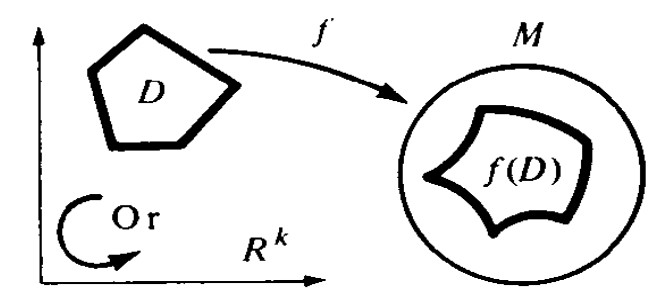
\includegraphics[width=0.35\linewidth]{tcc//img/arnold_celula.jpg}
    \caption{Representação de um poliedro singular $k$-dimensional \citep[Figura 150, pg. 184]{Arnold2013-bs}}
\end{figure}

\begin{definition}
    A integral de uma $k$-forma $\omega \in \Omega^k (M)$ sobre uma célula $\sigma = (D, f, Or)$ é dada por:
    \begin{equation*}
        \int_\sigma \omega := \int_D f^* \omega.
    \end{equation*}
    Ademais, se $c_k = \sum m_i \sigma_i$ é uma $k$-cadeia em $M$, então:
    \begin{equation*}
        \int_{c_k} \omega = \sum m_i \int_{\sigma_i} \omega.
    \end{equation*}
\end{definition}

Com a integração de formas sobre cadeias definida, é possível estender os teoremas integrais do cálculo vetorial para teoremas de integração de formas diferenciais sobre variedades. O mais geral deles é o \textit{Teorema de Stokes Generalizado}.

\begin{theorem}[Teorema de Stokes Generalizado]\citep[192-193]{Arnold2013-bs}
    Sejam $c$ uma $k$-cadeia em $M$ e $\partial c$ o seu bordo. Para $\omega$ uma $(k-1)$-forma em $M$, tem-se:
    \begin{equation*}
        \int_c d \omega = \int_{\partial c} \omega.
    \end{equation*}
\end{theorem}

A intuição por trás do teorema generalizado segue a mesma do teorema tradicional do cálculo vetorial: integrar o diferencial de um operador em um espaço é o mesmo que integrar o operador no bordo desse espaço.

Duas implicações imediatas do Teorema Generalizado vem da integração sobre formas fechadas e sobre formas exatas.

\begin{corollary}\label{corolario:integral_formas_fechadas}
    Se $\omega \in \Omega^k (M)$ é fechada, então $\int_{\partial c} \omega = 0$.
\end{corollary}

\begin{corollary}
    Se $\eta \in \Omega^k (M)$ é exata, então $\int_{\partial c} \eta = 0$.
\end{corollary}

Um último conceito utilizado em mecânica hamiltoniana é o de \textit{invariante integral}.

\begin{definition}
    Uma $k$-forma diferencial $\omega$ é dita um \textbf{invariante integral} de uma aplicação diferenciável $g: M \to M$ se para qualquer $k$-cadeia $c$ tem-se:
    \begin{equation*}
        \int_{gc} \omega = \int_c \omega.
    \end{equation*}
\end{definition}

%%%%%%%%%%%%%%%%%%%%%%%%%%%%%%%%%%%%%%%%%%%%%%%%%%%%%%%%%%%%%%%%%%%%%
% ESPACOS VETORIAIS SIMPLETICOS
%%%%%%%%%%%%%%%%%%%%%%%%%%%%%%%%%%%%%%%%%%%%%%%%%%%%%%%%%%%%%%%%%%%%%
\subsection{Espaços vetoriais simpléticos}
Iniciando o percurso na geometria simplética, trataremos de espaços vetoriais simpléticos, pois a extensão para outros espaços será mais simples. Seja $V$ um espaço vetorial $m$-dimensional sobre $\R$ e $\Omega \in \Lambda^2(V)$ uma 2-forma.

\begin{theorem}\label{teorema:standard_basis_symplectic}\citep{silva_lectures_2001}
    Existem vetores $\vet u_1, ..., \vet u_k$, $\vet e_1, ..., \vet e_n$, $\vet f_1, ..., \vet f_n$ que formam uma base de $V$ tais que
    \begin{align*}
        &\Omega(\vet u_i, \vet v) = 0,  &\forall i, \forall v \in V, \\
        &\Omega(\vet e_i, \vet e_j) = 0 = \Omega(\vet f_i, \vet f_j), &\forall i, j, \\
        &\Omega(\vet e_i, \vet f_j) = \delta_{ij}, &\quad \forall i, j,
    \end{align*}
    onde para $U = \{\vet u \in V | \Omega(\vet u, \vet v) = 0, \forall \vet v \in V\}$ tem-se $k=\dim U$, e $2n + k = \dim V$.
\end{theorem}

\begin{observation}
    Em notação matricial com respeito a essa base, podemos escrever:
    \begin{equation*}
        \Omega(\vet u,\vet v) = \vet u^t \begin{bmatrix}
            \vet 0 & \vet 0 \\ \vet 0 & \bm \Omega
        \end{bmatrix}
        \vet v,
    \end{equation*}
    onde $\bm \Omega = \begin{bmatrix}
        \bm 0 & \bm I \\ - \bm I & \bm 0
    \end{bmatrix}$ é a matriz simplética apresentada anteriormente.
\end{observation}

\begin{definition}
    A aplicação $\tilde \Omega: V \to V^*$ é a 1-forma definida por $\tilde \Omega (\vet v)(\vet u) = \Omega(\vet v,\vet u)$.
\end{definition}

\begin{definition}
    Dizemos que uma 2-forma geral $\Omega$ é \textbf{simplética} (ou \textbf{não degenerada}) se $\tilde \Omega$ é bijetiva, i.e., $\ker \tilde \Omega = \{0\}$. A aplicação $\Omega$ então é denominada como uma \textbf{estrutura simplética linear} sobre $V$, e $(V, \Omega)$ é chamado um \textbf{espaço vetorial simplético}.
\end{definition}

\begin{observation}
    Veja que $\ker \tilde \Omega = U$, então quando $\tilde \Omega$ é bijetiva, $\dim U = k = 0$, logo $\dim V = 2n$, portanto $V$ sempre tem dimensão par. Além disso, pelo teorema \ref{teorema:standard_basis_symplectic}, um espaço vetorial simplético $(V, \Omega)$ tem base $\vet e_1, ..., \vet e_n, \vet f_1, ..., \vet f_n$ satisfazendo
    \begin{equation*}
        \Omega(\vet e_i, \vet f_j) = \delta_{ij}, \quad \Omega(\vet e_i,\vet e_j) = 0 = \Omega(\vet f_i,\vet f_j).
    \end{equation*}
    Por fim, a notação matricial fica reduzida:
    \begin{equation*}
        \Omega(\vet u,\vet v) = \vet u^t \bm \Omega \vet v.
    \end{equation*}
\end{observation}

Diante de uma estrutura sobre um espaço vetorial, cabe perguntar que tipo de funções preservam tal estrutura. Estas funções são chamadas de \textit{simplectomorfismos}.

\begin{definition}
    Um \textbf{simplectomorfismo} $\varphi$ entre dois espaços vetoriais simpléticos $(V, \Omega)$ e $(V', \Omega')$ é um isomorfismo linear $\varphi: V \xrightarrow{\sim} V'$ tal que
    \begin{equation*}
        \varphi^* \Omega' = \Omega, 
    \end{equation*}
    onde $(\varphi^* \Omega')(\vet u,\vet v) = \Omega'(\varphi(\vet u),\varphi(\vet v))$. Se um simplectomorfismo existe, $(V, \Omega)$ e $(V', \Omega')$ são ditos \textbf{simplectomorfos}.
\end{definition}

Ser \textbf{simplectomorfo} é uma relação de equivalência no conjunto de todos os espaços vetoriais de mesma dimensão par. Isso vai além, pois podemos definir um \textbf{protótipo de espaço vetorial simplético} $(\R^{2n}, \Omega_0)$ tal que $\Omega_0$ tem a base
\begin{equation*}
    e_i = (\delta_{i,j})_{j=1,...,2n},
    \quad
    f_i = (\delta_{n+i,j})_{j=1,...,2n},
    \quad
    i = 1, ..., n,
\end{equation*}
e do teorema \ref{teorema:standard_basis_symplectic} decorre que qualquer espaço vetorial simplético $(V, \Omega)$ de dimensão $2n$ é simplectomorfo ao espaço $(\R^{2n}, \Omega_0)$. Então, ter a mesma dimensão par positiva também classifica classes de equivalência para a relação de ser simplectomorfo, de forma que todos os espaços simpléticos de mesma dimensão são simplectomorfos \citep[6]{silva_lectures_2001}.


%%%%%%%%%%%%%%%%%%%%%%%%%%%%%%%%%%%%%%%%%%%%%%%%%%%%%%%%%%%%%%%%%%%%%
% VARIEDADES SIMPLETICAS
%%%%%%%%%%%%%%%%%%%%%%%%%%%%%%%%%%%%%%%%%%%%%%%%%%%%%%%%%%%%%%%%%%%%%
\subsection{Variedades simpléticas}

Tomando uma variedade $M$ e um ponto $\vet p \in M$, o espaço tangente $T_{\vet p} M$ é um espaço vetorial. Uma vez que seja possível construir uma base simplética para uma estrutura $\omega$ em todo o fibrado tangente $TM$, $(T M, \omega)$ é um espaço vetorial simplético, e dizemos que $M$ admite uma \textbf{estrutura quase-simplética}.

É necessária uma restrição a mais para que $\omega$ seja uma estrutura simplética sobre $M$: $\omega$ deve ser fechado. Nesse caso, $\omega$ é dito uma \textbf{forma diferencial simplética} (ou simplesmente \textbf{forma simplética}) e com isso, podemos definir variedades simpléticas.

\begin{definition}
    Uma \textbf{variedade simplética} é um par $(M, \omega)$, onde $M$ é uma variedade e $\omega$ é uma forma simplética.
\end{definition}

Também é possível estender o conceito de \textit{simplectomorfismo} através de \textit{pullbacks}.

\begin{definition}[Simplectomorfismo]\label{def:simplectomorfismo}
    Sejam $(M_1, \omega_1)$ e $(M_2, \omega_2)$ variedades simpléticas e $\varphi: M_1 \to M_2$ um difeomorfismo. Dizemos que $\varphi$ é um \textbf{simplectomorfismo} se $\varphi^* \omega_2 = \omega_1$, onde $\varphi^*$ é o operador de \textbf{pullback}:
    \begin{equation*}
        (\varphi^* \omega_2)_{\vet p}(\vet u,\vet v) = (\omega_2)_{\varphi(\vet p)} (d \varphi_{\vet p}(\vet u), d \varphi_{\vet p}(\vet v)),
    \end{equation*}
    para cada $\vet u, \vet v \in T_{\vet p} M_1$, para cada $\vet p \in M_1$. 
\end{definition}

Uma implicação imediata da definição de simplectomorfismo é a invariância do volume.

\begin{theorem}\label{teorema:simplectomorfismo_invariante_integral}
    Se $g: M \to M$ é uma aplicação diferenciável, então $g$ é um simplectomorfismo se e somente se a forma simplética $\omega$ é um invariante integral de $g$.
\end{theorem}
\begin{Proof}
    Para a ida ($\Rightarrow$), veja que para uma $2$-cadeia $c$ tem-se:
    \begin{equation*}
        \int_{gc} \omega = \int_{c} g^* \omega = \int_{c} \omega.
    \end{equation*}
    Para a volta ($\Leftarrow$), temos que:
    \begin{equation*}
        \int_{gc} \omega = \int_{c} \omega
        \Longrightarrow
        \int_{c} g^* \omega = \int_{c} \omega
        \quad \therefore \quad
        g^* \omega = \omega.
    \end{equation*}
\end{Proof}

Uma vez que $\omega$ é uma 2-forma simplética, $\omega$ é o diferencial de uma 1-forma, e assim é definida pelo produto exterior de 1-formas. Isso significa que $\omega$ corresponde a um volume em seu domínio, então um simplectomorfismo é um difeomorfismo que conserva um volume em sua trajetória.

O conceito de espaços \textbf{simplectomorfos} é idêntico ao caso linear. Ainda, se tomamos $\R^{2n}$ com coordenadas $x_1, ..., x_n, y_1, ..., y_n$, a forma
\begin{equation*}
    \omega_0 = \sum_{i=1}^{n} dx_i \wedge dy_i
\end{equation*}
é simplética e logo $(\R^{2n}, \omega_0)$ é um espaço simplético, e da mesma forma que toda variedade de dimensão $n$ é localmente ``parecida'' com $\R^n$, toda $2n$-variedade simplética é localmente ``parecida'' com $(\R^{2n}, \omega_0)$, no sentido de que toda variedade $(M^{2n}, \omega)$ é localmente simplectomorfa a $(\R^{2n}, \omega_0)$. Isso decorre do \textbf{teorema de Darboux} e foge do escopo deste trabalho, mas os detalhes podem ser encontrados em \cite[7]{silva_lectures_2001}.

Uma forma prática de caracterizar simplectomorfismos dentro de um mesmo espaço é através da fórmula mágica de Cartan, o teorema \ref{teorema:formula_magica_cartan}.

\begin{theorem}\label{teorema:simplectomorfismo_e_lie}
    Sejam $X$ um campo vetorial suave em uma variedade simplética $(M, \omega)$, com fluxo associado $\varphi_t$ para algum ponto $\vet p \in M$. O fluxo $\varphi_t$ é um simplectomorfismo se, e só se, $\mathcal L_X \omega = 0$.
\end{theorem}
\begin{Proof}
    Pela definição \ref{def:simplectomorfismo}, queremos provar que $\varphi_t^* \omega = \omega \Leftrightarrow \mathcal L_X \omega = 0$.
    
    Para o lado ($\Rightarrow$), se $\varphi_t$ é um simplectomorfismo, tem-se por definição:
    \begin{equation*}
        \mathcal L_X \omega = \der{}{t}\bigg\rvert_{t=0} \varphi_t^* \omega
        = \der{}{t}\bigg\rvert_{t=0} \omega = 0.
    \end{equation*}
    Já para ($\Leftarrow$) Uma vez que $\varphi_{s_1} \circ \varphi_{s_2} = \varphi_{s_1 + s_2}$ (pela definição de fluxo), segue que
    \begin{equation*}
        \varphi_\lambda^* (\mathcal L_X \omega)
        = \varphi_\lambda^* \left(\der{}{t}\bigg\rvert_{t=0} \varphi_t^* \omega\right) 
        = \der{}{t}\bigg\rvert_{t=0} \varphi_{t+h}^* \omega
        = \der{}{t}\bigg\rvert_{t=\lambda}\varphi_t \omega.
    \end{equation*}
    Por hipótese, temos que $\mathcal L_X \omega = 0$, então
    \begin{equation*}
        \der{}{t}\bigg\rvert_{t=\lambda} \varphi_t^* \omega = 0, \quad \forall \lambda \in \R,
    \end{equation*}
    o que significa que a aplicação $\mu(\lambda) = \varphi_\lambda^* \omega$ é constante. Veja que
    \begin{equation*}
        \mu(0) = \varphi_0^* \omega = \omega \circ \varphi_0 = \omega 
        \Rightarrow
        \varphi_t^* \omega = \omega.
    \end{equation*}
\end{Proof}

Uma variedade simplética já conhecida neste momento é o \textit{fibrado cotangente} $T^* M$. Para coordenadas locais $(\vet q, \vet p)$, tomamos uma 1-forma $\omega^1 = \vet p d \vet q$. A partir disso, uma 2-forma exata natural é $\omega^2 = d \omega^1$, e que por ser exata é fechada, e portanto simplética. A 2-forma $\omega^2$ é dada por
\begin{equation*}
    \omega(f,g) = (d \vet q \wedge d \vet p)(f,g) = \derpar{f}{\vet q} \derpar{g}{\vet p} - \derpar{f}{\vet p} \derpar{g}{\vet q} = \nabla^t f \bm \Omega \nabla g,
\end{equation*}
onde $\bm \Omega$ é a matriz simplética. Com isso, agora é possível estudar os campos hamiltonianos e sua relação com a geometria simplética.

\subsection{Campos hamiltonianos}

Os campos hamiltonianos são um tipo de campo simplético com uma propriedade a mais: a 2-forma é exata.

\begin{definition}[Campo hamiltoniano]
    Sejam $X$ um espaço vetorial em uma variedade simplética $(M, \omega)$ e $H: M \to \R$ uma função suave. Dizemos que $X$ é um \textbf{campo hamiltoniano} se $\iota_X \omega = dH$ é exato. O campo $X$ é denotado por $X_H$ devido a sua relação com $H$ e dizemos que $(M, \omega, H)$ é um \textbf{sistema hamiltoniano}.
\end{definition}

Conforme o teorema \ref{teorema:simplectomorfismo_e_lie}, é fácil ver que todo campo hamiltoniano é necessariamente simplético, ou seja, o fluxo associado é um simplectomorfismo.

\begin{corollary}
    Todo campo hamiltoniano $X_H$ é simplético.
\end{corollary}
\begin{Proof}
    Pela fórmula de Cartan, temos que
    \begin{equation*}
        \mathcal L_{X_H} \omega = \iota_{X_H} (d \omega) + d (\iota_{X_H} \omega) = 0 + d(dH) = 0, 
    \end{equation*}
    pois $d \omega = 0$ ($\omega$ é simplético) e $\iota_{X_H} \omega = dH$. Pelo teorema \ref{teorema:simplectomorfismo_e_lie}, o fluxo $\varphi_t$ associado ao campo hamiltoniano $X_H$ é um simplectomorfismo.
\end{Proof}

Uma vez que o fluxo hamiltoniano é simplético, vale o teorema \ref{teorema:simplectomorfismo_invariante_integral}, então há também a conservação do volume. Isso é uma forma simplética de expressar o que já havia sido visto pelo teorema \ref{teorema:hamiltoniano_volume}, também chamado de \textbf{teorema de Liouville}. Essa conservação está ligada diretamente com a existência de integrais primeiras, e em particular $H$  é uma integral primeira para o fluxo $\varphi_t$.

\begin{proposition}
    A função $H$ é uma integral primeira do fluxo hamiltoniano $\varphi_t$.
\end{proposition}
\begin{Proof}
    Pela definição de $dH$, temos que:
    \begin{equation*}
        dH(X_H) = \iota_{X_H} \omega (X_H) = \omega(X_H, X_H) = 0.
    \end{equation*}
\end{Proof}

De fato, toda integral primeira do fluxo hamiltoniano terá campo tangente anulado por $dH$.

\begin{proposition}
    Seja $f$ uma função em $M$. $f$ é uma integral primeira para o fluxo hamiltoniano $\varphi_t$ se, e somente se, $dH(X_f) = 0$, onde $X_f = df$.
\end{proposition}
\begin{Proof}
    Se $f$ é uma integral primeira para $\varphi_t$, então
    \begin{equation*}
        \der{}{t} f(\varphi_t) = X_f \der{}{t} \varphi_t = dH (X_f) = 0.
    \end{equation*}
    A volta é análoga.
\end{Proof}

Ademais, um operador bastante presente na mecânica hamiltoniana é o \textit{colchete de Poisson}.

\begin{definition}
    Seja $(M, \omega)$ uma variedade simplética. O colchete de Poisson $\{\cdot,\cdot\}$ é um operador bilinear definido por
    \begin{equation*}
        \{f, g\}
        = - \iota_{X_f} \iota_{X_g} \omega 
        = \omega(X_f, X_g)
        = (\nabla f)^t \bm \Omega (\nabla g).
    \end{equation*}
\end{definition}

Com essa notação, é possível reescrever o resultado anterior sobre integrais primeiras: uma função $f$ é uma integral primeira para o fluxo hamiltoniano com função hamiltoniana $H$ se, e só se, $\{H, f\} = 0$. Além disso, se $f$ é uma função no espaço de fases, então
\begin{equation*}
    \der{}{t} f = \derpar{f}{t} + \{f, H\}.
\end{equation*}

Por fim, por maior que seja a diversidade de funções hamiltonianas, as que interessam neste trabalho são as cujo campo $X_H$ é dado por
\begin{equation*}
    X_H = \bm \Omega dH,
\end{equation*}
onde $\bm \Omega$ é a matriz simplética, e o espaço em questão é $(T^*M, \omega^2)$, com coordenadas $(\vet q, \vet p)$ e 2-forma associada. Isso significa, em particular, que
\begin{equation*}
    \{f, g\} = Df^t \bm \Omega Dg = \sum_i \derpar{f}{q_i}\derpar{g}{p_i} - \derpar{f}{p_i}\derpar{g}{q_i}.
\end{equation*}

Com essa notação, também é possível reescrever as equações de Hamilton (conforme teorema \ref{teorema:equacoes_hamilton}):
\begin{equation}\label{eq:poisson_hamilton_equacoes}
    \begin{cases}
        \dvet q(t) = \{\vet q, H\}, \\
        \dvet p(t) = \{\vet p, H\},
    \end{cases}
    \quad \text{ ou } \quad
    \dot \varphi(t) = \{\varphi, H\},
\end{equation}
onde $\varphi(t) = (\vet q(t), \vet p(t))$ é o fluxo hamiltoniano. Além disso, qualquer sistema de \textit{coordenadas canônicas} pode ser identificado através do colchete de Poisson: se $(\vet u, \vet v)$ é um par de coordenadas canônicas então
\begin{equation}\label{eq:poisson_coordenadas_canonicas}
    \{\vet u_a, \vet u_b \} = 0,
    \quad
    \{\vet v_a, \vet v_b \} = 0,
    \quad
    \{\vet u_a, \vet v_b \} = \delta_a^b.
\end{equation}
Observe que estas são as mesmas propriedades esperadas para uma \textit{base} de um espaço vetorial simplético, como no teorema \ref{teorema:standard_basis_symplectic}.

%%%%%%%%%%%%%%%%%%%%%%%%%%%%%%%%%%%%%%%%%%%%%%%%%%%%%%%%%%%%%%%%%%%%%
% TRANSFORMACOES CANONICAS
%%%%%%%%%%%%%%%%%%%%%%%%%%%%%%%%%%%%%%%%%%%%%%%%%%%%%%%%%%%%%%%%%%%%%
\subsection{Transformações canônicas}
Nesta última seção, é melhor explorado o significado do teorema \ref{teorema:simplectomorfismo_invariante_integral}. Os simplectomorfismos, caracterizados por terem a forma simplética como invariante integral, são também chamados de \textit{transformações canônicas}. A preservação das equações de Hamilton é uma consequência sob a aplicação de transformações canônicas, o que às vezes é mais prático de se testar do que a teoria simplética vista. Nesta seção, considere uma aplicação $\vet z \mapsto \vet w$, onde $\vet z = (\vet q, \vet p)$ e $\vet w = (\vet Q, \vet P)$, e dois campos hamiltonianos $V_H$ e $V_K$ associados de maneira respectiva.

\begin{definition}[Transformação canônica]
    Dizemos que a transformação $\vet z \mapsto \vet w$ é \textbf{canônica} se $H(\vet z) = K(\vet z'(\vet z))$ e se preserva as equações de Hamilton, isto é:
    \begin{equation*}
        \dvet z = \bm \Omega \nabla_{\vet z} H
        \longrightarrow
        \dvet z' = \bm \Omega \nabla_{\vet z'} K.
    \end{equation*}
\end{definition}

A partir da definição de transformação canônica, é possível deduzir uma forma prática de validar a simpleticidade de aplicações.

\begin{theorem}\label{teorema:simpleticidade_matricial}
    Uma aplicação $\vet z \mapsto \vet w$ é canônica se, e só se, sua matriz jacobiana
    \begin{equation*}
        \bm J = \derpar{(\vet Q, \vet P)}{(\vet q, \vet p)}
    \end{equation*}
    atende a seguinte condição:
    \begin{equation}\label{eq:simpleticidade_matricial_1}
        \bm J \bm \Omega \bm J^t = \bm \Omega.
    \end{equation}
\end{theorem}
\begin{Proof}
    Uma vez que $H(\vet z) = K(\vet w(\vet z))$, então $\nabla_{\vet z} H = \bm J^t \nabla_{\vet w} K$. Dessa forma,
    \begin{equation*}
        \dvet w 
        = \bm J \dvet z 
        = \bm J (\bm \Omega \nabla_{\vet z} H)
        = \bm J \bm \Omega \bm J^t \nabla_{\vet w} K
        = \bm \Omega \nabla_{\vet w} K,
    \end{equation*}
    sendo a última passagem por definição. Assim, a equação \ref{eq:simpleticidade_matricial_1} é necessária para que a aplicação seja canônica e vice-versa. É fácil ver que uma vez que esteja atendida, também é suficiente para garantir que $\vet z \mapsto \vet w$ se encaixa na definição de aplicação canônica.
\end{Proof}

\begin{corollary}
    Uma formulação equivalente a (\ref{eq:simpleticidade_matricial_1}) é:
    \begin{equation}\label{eq:simpleticidade_matricial_2}
        \bm J \bm \Omega \bm J^t \bm \Omega^t = \bm I.
    \end{equation}
\end{corollary}
\begin{Proof}
    A matriz $\bm \Omega$ é ortonormal, então $\bm \Omega^{-1} = \bm \Omega^t$.
\end{Proof}

Pelo teorema \ref{teorema:simpleticidade_matricial}, a aplicação ser canônica equivale a preservar o colchete de Poisson: para qualquer $u, v$, temos
\begin{equation*}
    \{ u, v \}_{\vet z}
    = (\nabla_{\vet z} u)^t \bm \Omega (\nabla_{\vet z} v)
    = (\nabla_{\vet w} u)^t \bm J \bm \Omega \bm J^t (\nabla_{\vet w} v)
    = (\nabla_{\vet w} u)^t \Omega (\nabla_{\vet w} v)
    = \{u, v \}_{\vet w}.
\end{equation*}

Mais ainda. A conservação do Parêntese de Poisson significa que a própria forma $\omega$ do sistema hamiltoniano está sendo conservada. Pela definição (\ref{def:simplectomorfismo}), as transformações canônicas são simplectomorfismos.

Com essa nova notação e novos conceitos, as equações de Hamilton no teorema \ref{teorema:equacoes_hamilton} ganham uma base teórica mais sólida, se definindo sobre espaços com estruturas bem definidas e específicas o suficiente para fornecer resultados numéricos; observar a variação numérica de um valor que deveria ser conservado teoricamente durante uma trajetória fornece informações sobre a razoabilidade de uma simulação, por exemplo. Isso será visto com mais detalhes no capítulo \ref{capitulo:metodos_numericos}.
% O problema de N-corpos (PNC) consiste de um sistema mecânico cujo movimento é descrito por um sistema de equações diferenciais ordinárias de segunda ordem, cuja solução tem existência local garantida no espaço euclidiano sem as singularidades (VOLCHAN). O PNC tem algumas propriedades imanentes garantidas por qualquer potencial V_k de grau k, como: energia total, momento linear total, momento angular total, centro de massas (integrais primeiras), redimensionamento e momento de inércia, o que fornece também duas relações interessantes: a relação de Distanciamentos e a relação de Lagrange-Jacobi (VOLCHAN). Formas de lidar com singularidades: regularização para colisões binárias; adicionando colisões elásticas para testar.

\chapter{O Problema de N-Corpos Gravitacional}\label{capitulo:pncg}

O Problema de N-Corpos Gravitacional (PNCG) é um sistema mecânico descrito por um conjunto de equações diferenciais ordinárias de segunda ordem, com existência e unicidade de solução garantidas localmente pelo Teorema de Existência de Unicidade. O PNCG possui algumas propriedades inerentes garantidas por seu potencial homogêneo, como a presença de uma integral primeira escalar e outras três vetoriais, a semelhança de soluções pelo redimensionamento anisotrópico, medidas de distanciamento e evolução da expansão.

Este capítulo é dedicado ao estudo do PNCG e de suas propriedades básicas citadas, sem, no entanto, se focar em questões demasiado específicas, como soluções analíticas para problemas de dois ou três corpos. São apresentados conceitos e propriedades gerais, além de uma introdução à Dinâmica de Formas sob o \textit{toy-model} de N-corpos.


\section{Enunciado}
Considere um conjunto de $N$ partículas dispostas no vácuo tridimensional ($\R^3$, digamos), cada uma com massa $m_a$, posição $\vet q_a$ e velocidade $\vet v_a$, para $a = 1, 2, ..., N$. A \textit{Lei da Gravitação Universal de Newton} fornece a seguinte função potencial suave:
\begin{equation}\label{eq:potencial_newtoniano}
    V = - \sum_{a < b} G \dfrac{m_a m_b}{r_{ab}},
    \quad
    r_{ab} = \norma{\vet q_a - \vet q_b},
\end{equation}
onde $G$ é a \textit{constante de gravitação universal}.

A partir de $V$, define-se um campo gradiente $\vet F = - \nabla V$ que gera as seguintes equações de movimento, conforme (\ref{eq:segunda_lei_de_newton}):
\begin{equation}\label{eq:mov_gravitacao}
    \begin{cases}
        \dvet q_a = \vet v_a, \\
        \dvet v_a = \dfrac{1}{m_a} \vet F_a = \sum_{b \neq a}^N G m_b \dfrac{\vet q_b - \vet q_a}{r_{ab}^3},
    \end{cases}
        \quad \forall a = 1, 2, ..., N.
\end{equation}

A existência e a unicidade das soluções das equações (\ref{eq:mov_gravitacao}) munidas de um conjunto de valores iniciais é garantida localmente em $(\R^3 / \Delta) \times \R^3$ pelo \textit{Teorema de Existência e Unicidade}, cuja demonstração pode ser encontrada em \citep[34-36]{Volchan:2007}. Aqui, $\Delta$ é o \textit{conjunto singular}, dado por
\begin{equation*}
    \Delta = \bigcup_{1 \leq i < j \leq N} \{(\vet q_1, ..., \vet q_N) \in \R^{3N}: \vet q_i = \vet q_j \}.
\end{equation*}

Observe que também é possível representar o problema em termos de posições e momentos conjungados, tomando $\vet p_a = m_a \vet q_a, \forall a$ e escrevendo as equações de Hamilton:
\begin{equation}
    \begin{cases}
        \dvet q_a = \derpar{H}{\vet p_a} = - \vet p_a / m_a, \\
        \dvet p_a = - \derpar{H}{\vet q_a} = \sum_{b \neq a}^N G m_a m_b \dfrac{\vet q_b - \vet q_a}{r_{ab}^3},
    \end{cases}
\end{equation}
onde como função Hamiltoniana toma-se a energia total:
\begin{equation*}
    H (\vet q, \vet p) = T(\vet p) + V(\vet q).
\end{equation*}

\section{Integrais primeiras}
O PNCG tridimensional possui dez integrais primeiras, cada uma correspondente a uma simetria dentro do sistema.

\begin{theorem}
    O PNCG possui como integrais primeiras não-triviais a energia total $E$ (correspondente à invariância temporal), momento angular total $\vet J$ (correspondente à invariância sob rotações), o momento linear total $\vet P$ e a trajetória $\vet G(t)$ do centro de massas $\vet q_{cm}$ (correspondentes à invariância sob translações).
\end{theorem}
\begin{Proof}
    Para a energia total, a demonstração já foi feita no Teorema \ref{teorema:energia_total}.

    Para o momento linear total $\vet P = \sum_{a=1}^N \vet p_a$, basta aplicar a definição \ref{def:integral_primeira}:
    \begin{equation*}
        \der{\vet P}{t} = \sum_{a=1}^{N} \der{\vet p_a}{t} = \sum_{a=1}^N \vet F_a = \vet 0,
    \end{equation*}
    pois o sistema é fechado.

    Para a trajetória do centro de massas, temos:
    \begin{equation}
        \vet G(t) = M \vet q_{cm} - t \vet P
        \Rightarrow
        \der{G}{t} = M \dfrac{\vet P}{M} - \vet P = \vet 0.
    \end{equation}
    No caso em que $\vet P = \vet 0$, a conservação de $G(t)$ equivale à conservação de $\vet q_{cm}$.

    Por fim, o momento angular total:
    \begin{equation}
        \der{\vet J}{t} 
        = \sum_{a=1}^N \vet q_a \times \dvet p_a
        = \sum_{a=1}^N \sum_{b\neq a}^{N} \dfrac{G m_a m_b}{r_{ab}^3} \vet q_a \times \vet q_b = \vet 0.
    \end{equation}
\end{Proof}

O fato de o centro de massas do Problema ter uma rota linear e seu momento generalizado ($\vet P$) ser uma integral primeira significa que se o centro de massas partir da origem e o momento linear total for nulo, o sistema não deverá se mover. Isso é particularmente interessante para simulações numéricas, mas mesmo analiticamente ainda é uma propriedade que facilita o estudo.

\section{Questões de escala}
Nas simulações numéricas diretas de gravitação (ou seja, integrando diretamente as equações de movimento do PNCG), uma questão fundamental que aparece é a da escolha de unidades de medida padrão, de modo a garantir que diferentes simulações possam ser comparáveis. Alguns padrões foram definidos por \cite{aarseth_gravitational_2003} e são aplicados nos códigos NBODY \citep{NBODY}, e serão vistos com mais cuidados na seção de simulação. Para fins teóricos, a princípio, é possível obter algumas relações acerca da medida dos sistemas de partículas e das órbitas.

Para começar, para cada problema de valor inicial do PNCG, é possível obter uma família infinita de órbitas idênticas a menos de um fator de escala anisotrópico. Isso significa que através de uma aplicação linear contínua, soluções são enviadas em soluções.

\begin{theorem}[Similaridade dinâmica]\label{teorema:similaridade_dinamica}
    As equações de movimento do PNCG satisfazem a similaridade dinâmica: se $(\vet q(t), \vet p(t))$ são órbitas do problema de N-corpos, o redimensionamento anisotrópico
    \begin{equation*}
        \tilde{\vet q}(\tilde t) = \alpha \vet q (t),
        \quad
        \tilde t = \alpha^{3/2} t,
        \quad
        \alpha > 0
    \end{equation*}
    das distâncias e do tempo newtoniano leva soluções $(\vet q(t), \vet p(t))$ em soluções $(\tilde{\vet q}(\tilde t), \tilde{\vet p}(\tilde t))$.
\end{theorem}
\begin{Proof}
    Considere um potencial geral homogêneo de grau $k$ e a mudança de coordenadas $\tilde{\vet q_a} = \alpha \vet q_a$, que implica em $\tilde t = \beta t$, para algum $\beta$ e então $\tilde{\vet p_a} = \alpha \vet p_a / \beta$. Com as novas coordenadas, temos a energia total
    \begin{equation*}
        H(\beta t, \alpha \vet q, \alpha \vet p / \beta) = \dfrac{\alpha^2}{\beta^2} T(\vet p) + \alpha^k V(\vet q).
    \end{equation*}
    Os sistemas são similarmente dinâmicos se $\beta$ for tal que podemos escrever $H(\tilde t, \tilde{\vet q}, \tilde{\vet p}) = \alpha^k H(t, \vet q, \vet p)$ (pois soluções são enviadas em soluções pelo redimensionamento). Decorre então que
    \begin{equation*}
        \alpha^k = \dfrac{\alpha^2}{\beta^2} \Rightarrow \beta = \alpha^{1-k/2}.
    \end{equation*}
    No PNCG temos que $k=-1$, e portanto $\tilde{\vet q_a} = \alpha \vet q_a$, $\tilde{\vet p_a} = \alpha^{-1/2} \vet p_a$ e $\tilde t = \alpha^{3/2} t$.
\end{Proof}

Observe que num problema de 2 corpos no qual um se encontra fixado e o outro sob uma órbita elíptica, se tomamos a distância $\ell$ entre os corpos e aplicamos a similaridade dinâmica obtemos:
\begin{equation*}
    \tilde \ell = \alpha \ell \Rightarrow \tilde \ell / \ell  = \alpha.
\end{equation*}
Isso significa que
\begin{equation*}
    \tilde t = \alpha^{3/2} t \Rightarrow \left(\dfrac{\tilde t}{t}\right)^2 = \left(\dfrac{\tilde \ell}{\ell}\right)^3,
\end{equation*}
o que é a chamada \textit{Terceira Lei de Kepler}. O que o teorema \ref{teorema:similaridade_dinamica} faz, dessa forma, é mostrar que é possível ignorar as escalas, em certo sentido, não apenas para $N=2$ mas para qualquer valor de $N$. Isso é explorado na seção \ref{secao:dinamica_de_formas}.

Além de redimensionar as órbitas, é particularmente interessante medir sua distância em função do tempo tendo em conta que aproximações tendem a gerar instabilidades numéricas. Uma medida para isso é dada pelo \textit{momento de inércia do centro de massas}.

\begin{definition}[Momento de inércia]\label{def:momento_inercia}
    O momento de inércia do centro de massas do PNCG é dado por:
    \begin{equation*}
        I 
        = \sum_{a=1}^{N} m_a \norma{\vet q_a - \vet q_{cm}}^2
        = \dfrac{1}{M} \sum_{a < b} m_a m_b \norma{\vet q_a - \vet q_b}^2
        =  R^2.
    \end{equation*}
\end{definition}

O observável $I$ pode ser interpretado como um tipo de \textit{variância} (no sentido estatístico) do sistema, uma vez que mede a dispersão das partículas em relação a um referencial (nesse caso, o centro de massas), sendo $R$, por sua vez, o \textit{desvio padrão}. Na perspectiva do sistema como um todo, $I$ mede a dilatação espacial. Sua taxa de variação em relação ao tempo fornece a quantidade de movimento (ou \textit{momento}, conforme nomeado por \cite{Barbour2003_scale_invariant_gravity}) da dilatação do sistema.

\begin{definition}[Momento de dilatação]
    O momento de dilatação do PNCG é proporcional à derivada do momento de inércia:
    \begin{equation*}
        D := \dfrac{1}{2} \der{I}{t} = \sum_{a=1}^{N} \vet q_a \cdot \vet p_a.
    \end{equation*}
\end{definition}

A variação do momento de dilatação oferece uma relação fundamental do PNCG, chamada \textit{identidade de Lagrange-Jacobi}.

\begin{theorem}[Identidade de Lagrange-Jacobi]\label{teorema:lagrange_jacobi}
    A segunda derivada do momento de inércia do PNCG é dada por:
    \begin{equation}
        \ddot I = 4 E - 2 V.
    \end{equation}
    No geral, se $V$ é homogêneo de grau $k$, então
    \begin{equation}
        \ddot I = 4 E - 2 (2 + k) V.
    \end{equation}
\end{theorem}
\begin{lemma}[Teorema de Euler para funções homogêneas]\label{lema:euler}
    Considere uma função $f$ homogênea de grau $k$ em um aberto $A \subseteq \R^n$. Então $k f(\vet x) = \prodint{x}{\nabla f(\vet x)}$, para todo $\vet x \in A$.
\end{lemma}
\begin{Proof}
    Como $f$ é homogênea de grau $k$, então
    \begin{equation*}
        f(\lambda \vet x) = \lambda^k f(\vet x).
    \end{equation*}
    Tomando $\vet u = \lambda \vet x$ e derivando dos dois lados em relação a $\lambda$, temos:
    \begin{equation*}
        \sum_{i=1}^n \derpar{f}{u_i} \der{u_i}{\lambda} = \sum_{i=1}^n x_i \derpar{f}{u_i} = k \lambda^{k-1} f(\vet x).
    \end{equation*}
    Em particular, tomando $\lambda = 1$ (pois $\lambda$ é qualquer), tem-se:
    \begin{equation*}
        k f(\vet x) = \prodint{\vet x}{\nabla f(\vet x)}.
    \end{equation*}
\end{Proof}
\begin{Proof}
    (do teorema). Uma vez que $\dot I = 2D$, basta derivar novamente:
    \begin{equation*}
        \ddot I (t) = 2 \der{D}{t} = 2 \sum_{a=1}^N \dvet q_a \cdot \vet p_a + 2 \sum_{a=1}^{N} \vet q_a \cdot \dvet p_a = 4 T - 2 \sum_{a=1}^{N} \prodint{\vet q_a}{\nabla_{\vet q_a} V}.
    \end{equation*}
    Se $V$ é homogêneo de grau $k$, então podemos aplicar o lema \ref{lema:euler}:
    \begin{equation*}
        \ddot I(t) = 4 T - 2 k V = 4 E - 2 (2+k) V,
    \end{equation*}
    sendo $k = -1$ o caso newtoniano.
\end{Proof}

A Identidade de Lagrange-Jacobi é útil uma vez que $-2V$ é um valor necessariamente positivo, o que significa que a dilatação do sistema de partículas depende fortemente da energia total do sistema, que é constante. Escolher valores iniciais de modo a obter $E \geq 0$, por exemplo, implica que $\ddot I (t) > 0$, então $I(t)$ assume um formato côncavo para cima (com um mínimo global), e portanto o sistema possui um momento de contração máxima seguido de uma expansão indefinida, tanto do ponto de vista em que o tempo $t$ cresce quanto para quando $t$ decresce. Isso, novamente, é utilizado pela Dinâmica de Formas e é explorado com mais detalhes na seção \ref{secao:dinamica_de_formas}.

Uma outra relação importante no PNCG fornece estimativas para as separações máximas e mínimas dos corpos a partir de $R$ e de $V$, respectivamente.

\begin{theorem}\label{teorema:distanciamento}
    Sejam $q_{min} = \min_{j \neq k} q_{jk}$ e $q_{max} = \max_{j \neq k} q_{jk}$ os distanciamentos mínimo e máximo entre as partículas, respectivamente, $m_0 = \min_a m_a$ e $M = \sum_{a=1}^{N} m_a$. Tem-se as seguintes relações:
    \begin{equation*}
        R \sqrt{\dfrac{2}{M}} \leq q_{max} \leq \dfrac{R \sqrt{M}}{m_0},
        \quad
        - \dfrac{G m_0^2}{V} \leq q_{min} \leq - \dfrac{G M^2}{2 V}.
    \end{equation*}
\end{theorem}
\begin{Proof}
     Começando por $q_{max}$, podemos escrever que
    \begin{equation}
        \dfrac{m_0^2}{2 M} q_{max}^2
        \leq
        \dfrac{m_0^2}{2 M} \sum_{a < b} r_{ab}^2
        \leq
        \dfrac{1}{2} I,
    \end{equation}
    e, analogamente:
    \begin{equation}
    \dfrac{1}{2} I \leq \left( \dfrac{1}{2 M} \sum_{a < b} m_a m_b \right) q_{max}^2 
    = \left( \dfrac{1}{4 M} \sum_{b=1}^{N} \sum_{a=1}^{N} m_a m_b \right ) q_{max}^2
    = \dfrac{M}{4} q_{max}^2. 
    \end{equation}
    Isso significa que
    \begin{equation}
        \dfrac{m_0^2}{M} q_{max}^2 \leq I \leq \dfrac{M}{2} q_{max}^2 
        \Rightarrow
        R \sqrt{\dfrac{2}{M}} \leq q_{max} \leq \dfrac{R\sqrt{M}}{m_0}.
    \end{equation}

    Da mesma forma, como $\frac{1}{2} M^2 \geq \sum_{a<b} m_a m_b$, temos que:
    \begin{equation}
        -V \leq \dfrac{G}{q_{min}} \sum_{a < b} m_a m_b \leq \dfrac{G}{2q_{min}} \sum_{b=1}^{N} \sum_{a=1}^{N} m_a m_b = \dfrac{G M^2}{2 q_{min}},
    \end{equation}
    e, ademais, vale que
    \begin{equation}
        -V \geq G \dfrac{m_a m_b}{r_{ab}} \geq \dfrac{G m_0^2}{r_{ab}}, \quad \forall 1 \leq a,b \leq N,
    \end{equation}
    e como para algum $a$ e $b$ vale que $r_{ab} = q_{min}$, temos que
    \begin{equation}
        -V \geq \dfrac{G m_0^2}{q_{min}}.
    \end{equation}
    Obtemos a relação:
    \begin{equation}
        - \dfrac{G M^2}{2 q_{min}} \leq V \leq - \dfrac{G m_0^2}{q_{min}},
    \end{equation}
    o que oferece a relação buscada (pois $V < 0$):
    \begin{equation}
        - \dfrac{G m_0^2}{V} \leq q_{min} \leq - \dfrac{G M^2}{2 V}.
    \end{equation}
\end{Proof}

Também é possível limitar o comportamento do momento angular usando a relação de Lagrange-Jacobi.

\begin{theorem}[Desigualdade de Sundman]
    Considere o momento angular total $\vet J$, o momento de inércia $I$ e a energia total $H$. Então
    \begin{equation*}
        \norma{\vet J}^2 \leq I (\ddot I - 2 H).
    \end{equation*}
\end{theorem}
\begin{Proof}
    Começamos pela desigualdade de Cauchy-Schwarz:
    \begin{align*}
        \norma{\vet J} 
        &\leq \sum_{a=1}^{N} m_a \norma{\vet q_a \times \vet p_a m_a^{-1}}
        \leq \sum_{a=1}^{N} m_a \norma{\vet q_a} \norma{\vet p_a m_a^{-1}} \\
        &= \sum_{a=1}^{N} (\sqrt{m_a} \norma{\vet q_a})(\sqrt{m_a}\norma{\vet p_a m_a^{-1}})
        \leq \sqrt{\sum_{a=1}^{N} m_a \norma{\vet q_a}^2} \sqrt{\sum_{a=1}^{N} m_a^{-1} \norma{\vet p_a}^2} \\
        &= \sqrt{2 I T}.
    \end{align*}
    Pela relação de Lagrange-Jacobi, $2T = \ddot I - 2 H$, então obtém-se o esperado.
\end{Proof}

\section{Colisões}\label{section:pncg_colisoes}

O intervalo maximal de soluções do PNCG não necessariamente se estende para toda a reta, pois existem circunstâncias em que a solução é interrompida abruptamente. Um exemplo de caso é quando duas trajetórias se interceptam em um dado instante comum, o que fisicamente significa que dois corpos colidiram. 

Lidar com essas situações é também necessário do ponto de vista numérico, pois muitas vezes não se pretende encerrar uma simulação quando dois corpos colidirem. Além disso, mesmo aproximações muito intensas são capazes de instabilizar numericamente os métodos devido aos erros de ponto flutuante, então, ainda que duas trajetórias não colidam exatamente, pode ser numericamente interessante lidar com a aproximação supondo que houve colisão.

De fato, tais situações de aproximação são de maior interesse, pois é conhecido que o conjunto de condições iniciais que leva a uma colisão em tempo finito tem medida de Lebesgue zero \citep{Saari1971}. Então, embora isso não implique na impossibilidade de que ocorram, colisões \textit{verdadeiras} são raras.

Existem algumas formas de tratar esses casos, como por meio de regularizações ou mesmo com amortecedores no potencial, como será discutido na seção \ref{section:simulacao_colisoes}. Uma possibilidade aqui proposta é a de adicionar colisões perfeitamente elásticas. As colisões perfeitamente elásticas (ou CPE) são aquelas em que não há deformação dos objetos e a energia cinética é conservada. Essa é uma possível vantagem sobre os outros métodos, uma vez que não compromete a estrutura simplética de sistemas hamiltonianos.

Uma abordagem consiste em definir um parâmetro de densidade $\rho$, e uma vez que cada corpo tem massa, a densidade definirá um volume. Na suposição de que os corpos são perfeitamente esféricos, tem-se o raio
\begin{equation}
    r = \sqrt[3]{\dfrac{3 m}{4 \pi \rho}}.
\end{equation}

Além disso, um critério para garantir que dois corpos próximos de massas $m_1$ e $m_2$, posições $\vet q_1$ e $\vet q_2$ e velocidades $\vet v_1$ e $\vet v_2$, estão em rota de colisão é verificar se
\begin{equation*}
    \prodint{\vet q_2 - \vet q_1}{\vet v_2 - \vet v_1} \leq 0.
\end{equation*}

% Comecar a falar da fisica das colisoes

A dinâmica pós-colisão é definida da maneira que segue. Sejam as massas, posições e velocidades como anteriormente. Sejam também $\vec \pi$ o plano tangente de contato e $\vet N$ o versor normal ao plano:
\begin{equation}
    \vet N = \dfrac{\vet q_2 - \vet q_1}{\norma{\vet q_2 - \vet q_1}} = (n_1, n_2, n_3).
\end{equation}

\begin{figure}[H]
    \centering
    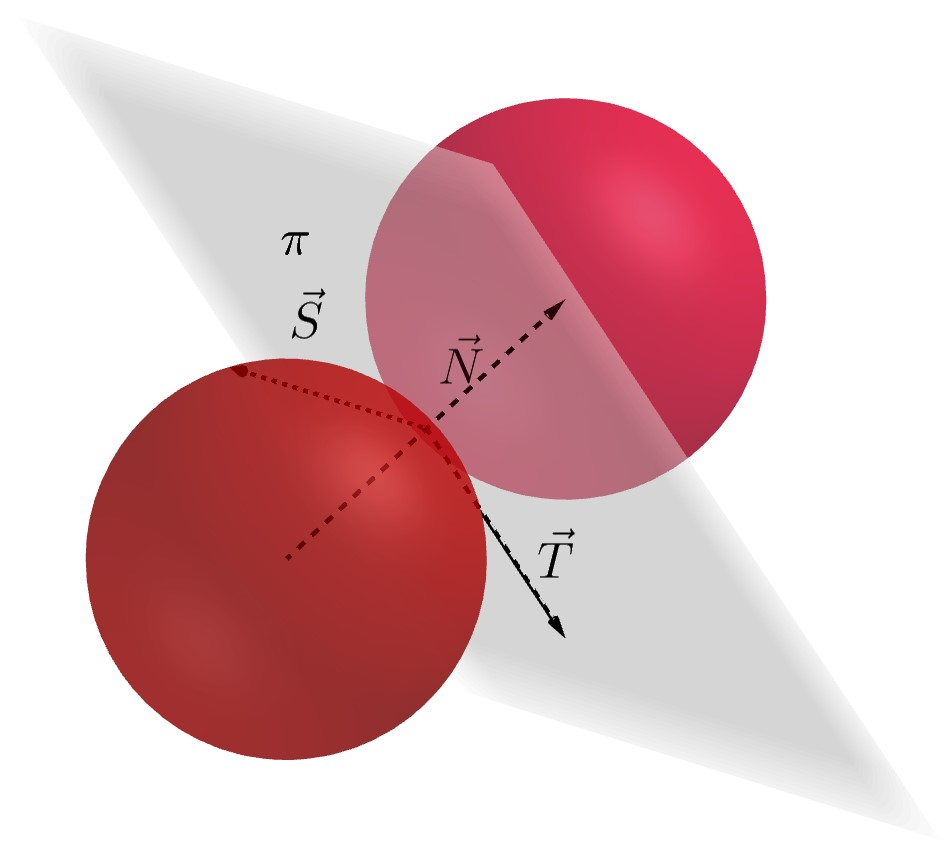
\includegraphics[width=4cm]{tcc/img/colisao_corrigida.jpg}
    \caption{Colisão entre dois corpos, plano tangente $\vet \pi$ e versores.}
    \label{fig:colisao-3d}
\end{figure}

Para obter os versores geradores do plano, basta tomar, por exemplo, os vetores
\begin{equation*}
    \vet T = \dfrac{(n_3, n_3,-n_1 - n_2)}{\norma{(n_3, n_3,-n_1 - n_2)}},
    \quad
    \vet S = \dfrac{\vet N \times \vet T}{\norma{\vet N \times \vet T}},
\end{equation*}
como na figura \ref{fig:colisao-3d}. Observe que $\vet T$ não é bem definido, uma vez que $n_1 = -n_2$ e $n_3 = 0$ gera $\vet T = \vet 0$. Na ocorrência desse caso, uma solução possível é utilizar outro vetor $\vet T$:
\begin{equation*}
    \vet T = \dfrac{(-n_2, n_1, 0)}{\norma{(-n_2, n_1, 0)}}.
\end{equation*}
Supondo que não ocorrem colisões reais, isto é, que $\vet N \neq \vet 0$ (o que, numericamente, é uma suposição válida), definimos $\vet S$ da mesma forma e o método que segue se mantém.

Com isso, as velocidades podem ser decompostas em relação ao plano tangente e em relação ao vetor normal:
\begin{align*}
    \vet v_1 &= \vet v_1^{\vet \pi} + v_1 \vet N,
    \\
    \vet v_2 &= \vet v_2^{\vet \pi} + v_2 \vet N.
\end{align*}

Uma vez que o sistema não contém rotações individuais, em uma colisão não há forças atuando nas direções do plano tangente, então a única alteração se dá nas componentes normais. Sendo $v_1'$ e $v_2'$ as novas velocidades normais, a colisão ser perfeitamente elástica implica na conservação do momento linear total e da energia cinética:
\begin{equation}\label{eq:colisoes_conservacao}
    \begin{cases}
        m_1 v_1 + m_2 v_2 = m_1 v_1' + m_2 v_2', \\
        m_1 v_1^2 + m_2 v_2^2 = m_1 v_1'^2 + m_2 v_2'^2.
    \end{cases}
\end{equation}

Do sistema de equações (\ref{eq:colisoes_conservacao}), decorre que
\begin{align*}
    v_1' &= \dfrac{v_1 (m_1 - m_2) + 2 m_2 v_2}{m_1 + m_2}, \\
    v_2' &= \dfrac{v_2 (m_2 - m_1) + 2 m_1 v_1}{m_1 + m_2}.
\end{align*}

Dessa forma, as novas velocidades após a colisão são:
\begin{align*}
    \vet v_1' = \vet v_1^{\vet \pi} + v_1' \vet N, \\
    \vet v_1' = \vet v_1^{\vet \pi} + v_1' \vet N.
\end{align*}

\begin{figure}[H]
    \centering
    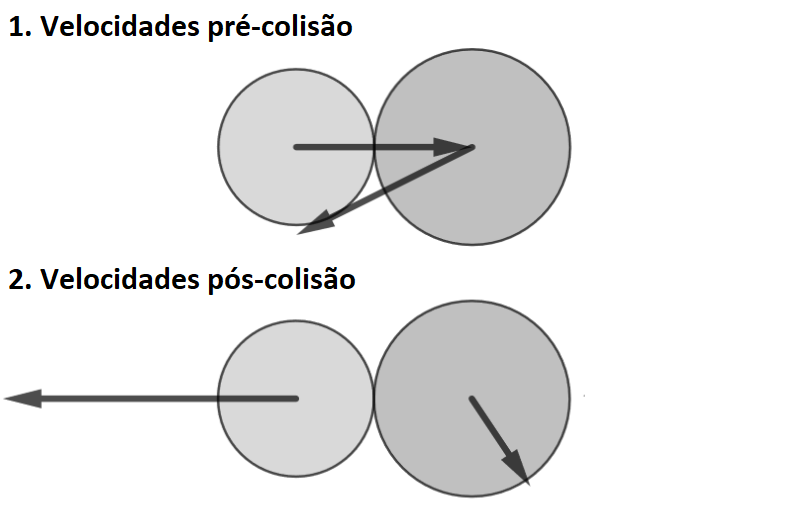
\includegraphics[width=8cm]{img/colisao_exemplo.png}
    \caption{Exemplo de colisão. Os tamanhos diferentes indicam massas diferentes.}
    \label{fig:colisao_exemplo}
\end{figure}

Na figura \ref{fig:colisao_exemplo} tem-se um exemplo de colisão entre dois corpos com massas diferentes. Como esperado, um corpo de massa menor sai da colisão com mais velocidade (e com sentido oposto), enquanto um de massa maior sai com menos velocidade (e com componente normal também no sentido oposto).

\section{Estabilidade}
% Falar um pouco da estabilidade e das ideias do momento de dilatação talvez. A princípio usar o capítulo do Volchan.

A principal motivação da última subseção foi obter uma forma conservativa de estender soluções do PNCG que são ``interrompidas''. Essa interrupção é, no sentido matemático, uma singularidade na órbita, o que limita o intervalo maximal para um tempo finito. O caso mais simples de interrupção é justamente uma colisão entre dois ou mais corpos.

\begin{definition}[Colisão]
    Diz-se que ocorre uma colisão no instante $t^*$ se cada $\vet q_j(t)$ tem limite finito quando $t \to t^*$, no sentido de que para algum $i \neq k$, $\vet q_i(t^*) = \vet q_k(t^*)$. Se para todo $i,k=1,2,...,N$ tem-se que $\vet q_i(t^*) = \vet q_k(t^*)$, então tem-se um \textbf{colapso total}.
\end{definition}

Apesar de ser uma exceção, o colapso total ocorre em situações interessantes para este trabalho. Decorre do teorema \ref{teorema:distanciamento} que se ele ocorre em algum instante $t = t^*$, então ele ocorre na origem. Para isso, basta ver pela definição \ref{def:momento_inercia} que $I(t^*) = 0$, então $q_{max} = 0$. Além disso, uma colisão total só ocorre em tempo finito.

\begin{proposition}
    Se ocorre o colapso total em $t=t^*$, então $t^* < +\infty$.
\end{proposition}
\begin{Proof}
    Suponha que $t^* = +\infty$. Como o colapso total ocorre na origem,
    \begin{equation*}
        \lim_{t \to +\infty} V(\vet q(t)) = - \infty
        \Rightarrow
        \lim_{t \to +\infty} \ddot I(t) = +\infty
    \end{equation*}
    através da identidade de Lagrange-Jacobi. Assim, existe $t_1 > 0$ de modo que para todo $t > t_1$ vale que $\ddot I(t) \geq 1$. Então:
    \begin{equation*}
        I(t) \geq \frac{1}{2} t^2 + c_1 t + c_2,
        \Rightarrow
        \lim_{t \to +\infty} I(t) = +\infty,
    \end{equation*}
    o que é uma contradição.
\end{Proof}

Outro ponto é que só ocorre o colapso total dentro de uma hipersuperfície específica do espaço de fases.

\begin{theorem}[Sundman-Weierstrass]
    Se ocorre o colapso total, então $\vet J = \vet 0$.
\end{theorem}

A demonstração pode ser encontrada em \citep[62-63]{Volchan:2007}. Um resultado importante também de Sundman é que se $\vet J \neq 0$, então não ocorrem colisões triplas. Na prática, através da regularização das colisões binárias, a solução de um problema com $\vet J \neq 0$ pode ter intervalo maximal estendido para toda a reta.

Nesse momento, qualquer definição de ``estabilidade'' das órbitas deve supor que não ocorre o colapso total, mas isso ainda não é suficiente. Um critério mais bem-definido proposto por Volchan é: para todo $i \neq j$ e todo $t \in \R$ e para uma constante $K > 0$,
\begin{enumerate}
    \item $r_{ij} \neq 0$;
    \item $r_{ij} \leq K$.
\end{enumerate}
Isto é, o sistema não só não cai sobre si mesmo, como também se mantém confinado em um cilindro de raio $K$. No caso de $\vet P = 0$, o sistema se encontra parado, então a restrição corresponde a uma esfera de raio $K$. Sistemas periódicos, por exemplo, atendem a essa propriedade.

De forma geral, Jacobi propôs uma condição necessária \citep[65]{Volchan:2007}.

\begin{theorem}[Critério de estabilidade de Jacobi]
    Uma condição necessária para que a solução seja estável é que a energia total seja negativa.
\end{theorem}
\begin{Proof}
    Como comentado anteriormente, se a energia é não-negativa então $I$ assume formato côncavo e é limitado inferiormente. Assim, $\lim_{t \to \infty} I(t) = +\infty$, então o tamanho do sistema não é limitado.
\end{Proof}

Para $N=2$, a condição é suficiente. Porém, isso não se estende para $N \geq 3$. Ainda assim, é possível obter outra condição necessária a partir da relação de Lagrange-Jacobi, ao que se denomina usualmente por \textbf{teorema do virial}.

\begin{theorem}[Teorema do virial]\label{teorema:virial}
    Uma condição necessária para que um sistema seja limitado é que
    \begin{equation*}
        \langle T \rangle_\tau = - \frac{1}{2} \langle V \rangle_\tau.
    \end{equation*}
\end{theorem}
\begin{Proof}
    O operador $\langle \cdot \rangle_\tau$ corresponde à média temporal no intervalo $[0, \tau]$. Pela identidade de Lagrange-Jacobi,
    \begin{equation*}
        \left\langle \der{D}{t} \right\rangle_{\tau}
        = 2 \langle T \rangle + \langle V \rangle.
    \end{equation*}
    Se um sistema é limitado então o momento de dilatação $D$ é limitado, e, uma vez que
    \begin{equation*}
        \left\langle \der{D}{t} \right\rangle_{\tau}
        = \frac{1}{\tau} \int_0^\tau \der{D}{t} dt = \dfrac{D(\tau) - D(0)}{\tau},
    \end{equation*}
    então
    \begin{equation*}
        \lim_{\tau \to \infty} \left| \left\langle \der{D}{t} \right\rangle_{\tau} \right| \leq \lim_{\tau \to \infty} \dfrac{D_{max} - D_{min}}{\tau} = 0.
    \end{equation*}
    Assim, vale $\langle T \rangle_\tau = - \frac{1}{2} \langle V \rangle_\tau$.
\end{Proof}

É possível estimar uma região do espaço em que vale o equilíbrio (de virial). Considere $N$ partículas dispostas com distância média $R_V$ com massa média $\bar m = M / N$, para $M = \sum_{a=1}^N m_a$. Temos que:
\begin{equation*}
    V = - G \sum_{a < b} \dfrac{m_a m_b}{r_{ab}}
    \approx - G \sum_{a<b} \bar m^2 \dfrac{1}{R_V}
    = - G \dfrac{M^2}{N^2} \dfrac{N (N-1)}{2 R_V}
    = - G \dfrac{M^2}{2 R_V} \dfrac{N-1}{N}.
\end{equation*}
Para $N$ grande, temos que
\begin{equation}\label{eq:raio_virial}
    V \approx - \dfrac{G M^2}{2 R_V}
    \Rightarrow
    R_V \approx \dfrac{G M^2}{2 |V|}.
\end{equation}

Tal $R_V$ é chamado \textbf{raio de virial}. A busca por sistemas estáveis deve começar por sistemas com energia negativa e para os quais valem o teorema do virial, e o raio de virial é útil nesse sentido. Isso é utilizado na geração de valores iniciais na seção \ref{subsection:condicoes_aarseth}, com as condições iniciais propostas por \citep{aarseth_gravitational_2003}. 

Também pode ser razoável supor que o momento angular total seja não nulo se o propósito for buscar estabilidade com mais facilidade, embora isso não seja condição necessária.

\section{A Dinâmica de Formas}\label{secao:dinamica_de_formas}
A Dinâmica de Formas (SD, do inglês \textit{Shape Dynamics}) é uma teoria de gravitação baseada em \textit{relacionalismo}, isto é, os conceitos absolutos de \textit{espaço} e de \textit{tempo} são suprimidos para basear a física na relação entre os objetos em questão - no caso do PNCG, a relação entre os corpos.

Embora seja um modelo alternativo de gravitação, foi a partir dela que começamos o estudo do PNCG como um todo, através do artigo \cite{Barbour2014_identification}. Por isso, apresentamos nesta seção uma breve introdução à versão quantizada (em massas pontuais) da SD e alguns de seus resultados qualitativos, que na seção \ref{secao:simulacao_dinamica_de_formas} são revisitados e podem ser visualizados através de simulações numéricas.

Nesta seção, algumas demonstrações foram omitidas tendo em vista facilitar a leitura do texto. Estas se encontram no Apêndice \ref{apendice:demonstracoes_dinamica_de_formas}. Além disso, as referências utilizadas encontram-se citadas no texto, mas as principais são o artigo mencionado, \cite{barbour2013_gravitationaloriginarrowstime} e \cite{Barbour2014_solution}.

%%%%%%%%%%%%%%%%%%%%%%%%%%%%%%%%%%%%%%%%%
\subsection{Contextualização e motivação}

O objetivo da Dinâmica de Formas é fornecer um modelo de gravitação que comporte a compreensão mecânica do físico e filósofo Ernst Mach (1838-1916), na qual apenas as relações inter-partícula são \textit{reais}. Para o problema de N-corpos em $\R^{3N}$, tomamos o quociente pelas translações e rotações euclidianas, obtendo o \textit{espaço de configurações relativas} (ECR) machiano, de $3N-6$ dimensões, o que remove as posições e orientações absolutas. Mais ainda, é preciso quocientar o ECR também em relação a \textit{dilatações}, para remover qualquer influência de escalas. Nisso, obtemos o \textit{espaço de formas} $S$ com $3N-7$ dimensões. 

Observe que ao quocientar $\R^{3N}$ pelas translações, a mecânica vigente ainda é a mecânica newtoniana, uma vez que o potencial newtoniano é invariante sob translações. Já para rotações, a situação não é a mesma, sendo o momento angular um elemento crucial de subsistemas fechados do universo (como o Sistema Solar). O modelo, então, se baseia no pressuposto de que não há rotação global no universo, mas somente rotações locais de subsistemas \citep[264]{Barbour2012_sd_introduction}.

Nessa situação, se torna aplicável um princípio que, embora não tenha sido enunciado diretamente por Mach, decorre de sua filosofia \citep[139]{Assis:1998}, que é chamado de \textit{princípio de Mach} ou \textit{de Mach-Poincaré}:

\begin{definition}[Princípio de Mach-Poincaré]
    A especificação de um ponto e uma direção (\textbf{forma forte}) ou de um ponto e um vetor tangente (\textbf{forma fraca}) no espaço de formas $S$ determinam a evolução em $S$ de forma única. \citep[31]{Barbour2014_kepler_mach}
\end{definition}

É fato importante que como um modelo de gravidade aplicável, existe uma interseção entre a Dinâmica de Formas e a Relatividade Geral, ocorrendo quando a Relatividade Geral comporta o Princípio de Mach-Poincaré: universos espacialmente fechados (\citealp[157]{Einstein:1981}; \citealp[258]{Barbour2012_sd_introduction}).

De toda forma, há diversas consequências da SD que são interessantes para a física, desde o próprio modelo de gravitação até implicações para uma gravidade quântica \citep{Barbour2012_sd_introduction}. Para este trabalho, o que interessa é a formulação de setas do tempo relacionais, uma forma de observar a evolução de sistemas de N-corpos baseada somente no próprio sistema.

%%%%%%%%%%%%%%%%%%%%%%%%%%%%%%%
% PRIMEIRO, PRECISO FALAR DO POR QUE QUERER SETAS DO TEMPO
% - MUITOS QUEREM DESCREVER A EVOLUÇÃO UTILIZANDO A ENTROPIA. O CONCEITO ORIGINAL NÃO FAZ SENTIDO PARA O PNCG, POIS A GRAVIDADE É DOMINANTE, O UNIVERSO NÃO TEM PAREDES E UM VOLUME GLOBAL FAZ ENTENDER QUE EXISTE ALGO MAIOR PARA REFERENCIAR.
Uma seta do tempo é um observável que não apenas caracteriza a evolução de um sistema dinâmico, mas também fornece uma orientação, no sentido de determinar o que é \textit{passado} e o que é \textit{futuro}. Na física, a maioria das discussões de setas do tempo se baseia no crescimento da entropia, uma medida de ``dispersibilidade'' de um sistema. Porém, no caso de sistemas puramente gravitacionais e fechados, a entropia como seta do tempo é uma escolha bastante questionável por algumas razões. Por exemplo, a conceitualização original de entropia se baseia em partículas fechadas em um espaço confinado e em um volume total do espaço de fases; ambas as bases não se encaixam ao Universo enquanto um sistema máximo no qual a gravidade é a força dominante.

% - A IDEIA ENTÃO É ABSTRAIR TODAS AS ESTRUTURAS EXTERNAS DA DINÂMICA DO PROBLEMA. NO PNCG, SÃO A POSIÇÃO, ORIENTAÇÃO E TAMANHO EM UM REFERENCIAL INERCIAL E UM TEMPO EXTERNO. UMA HISTÓRIA DINÂMICA É UMA CURVA UNPARAMETRIZED EM S. AS EQUAÇÕES DE MOVIMENTO DO PNCG SÃO SIMETRICAS NO TEMPO, ENTÃO NÃO DEFINEM UMA ORIENTAÇÃO EM C. TAMBEM POR ISSO, ENTROPIA E OUTRAS SETAS NÃO FAZEM SENTIDO.

% - UMA SETA DIGNA ENTÃO PRECISA TER ORIGEM EM UMA ASSIMETRIA DENTRO DO ESPAÇO S

Voltando ao enunciado sobre o princípio de Mach, o que realmente caracteriza a dinâmica do PNCG está no espaço $S$. Porém, as equações de movimento de Newton são simétricas no tempo, e portanto incapazes de fornecer uma orientação para a evolução de uma órbita em $S$. Assim, uma seta do tempo para o PNCG precisa ser caracterizada por alguma assimetria dentro do próprio espaço de formas.

% - COMO A ESCALA (DEGREES OF FREDOM) É UNICA E TEM DIMENSÕES, DEPENDENDO DE UMA ESCALA EXTERNA DEFINIDA, É PRECISO QUE AS SHAPE DOF NÃO TENHAM ESSE PROBLEMA. ATRAVÉS DE UMA DEPARAMETRIZAÇÃO, TRANSFORMAMOS A VARIÁVEL DE ESCALA (R) EM UM HAMILTONIANO (LOG R) E O SEU MOMENTO CONJUGADO MONÓTONO (D) NO PARÂMETRO DE EVOLUÇÃO (t). RESTA O MENOR CONJUNTO DE VARIÁVEIS NECESSÁRIAS PARA DESCREVER O UNIVERSO OBJETIVAMENTE.

\subsection{Eliminação da escala}
Uma questão sobre o PNCG é que o sistema comporta escalas. No entanto, já foi apresentado que através do Teorema \ref{teorema:similaridade_dinamica} é possível ignorar a escala, uma vez que aplicar um redimensionamento anisotrópico sobre uma trajetória fornece um conjunto de trajetórias com dinâmicas iguais a menos da escala. Uma representação objetiva do problema precisa ser capaz de condensar esse conjunto infinito de trajetórias dinamicamente equivalentes em uma única órbita em $S$. 

Para isso, podemos utilizar a raiz quadrada do momento de inércia $R$, pois este representa um tipo de \textit{desvio padrão} do sistema. Nesse caso, é preciso balancear cada posição com relação a sua massa, aplicando a transformação:
\begin{equation}
    \vet \sigma_a = \dfrac{\sqrt{m_a}}{R} \vet q_a,
    \quad a = 1, 2, ..., N.
\end{equation}
Observe que $\vet \sigma_a$ é adimensional. Além disso, trata-se uma coordenada dentro de uma bola unitária espacial na origem de $S$, uma vez que, por exemplo, para $N=1$ tem-se:
\begin{equation*}
    \vet \sigma_a = \dfrac{\sqrt{m_a} \vet q_a}{\sqrt{m_a} \norma{\vet q_a}} = \dfrac{\vet q_a}{\norma{\vet q_a}},
\end{equation*}
e valores maiores de $N$ oferecem um denominador maior que o numerador.

Podemos obter momentos conjugados para as coordenadas $\vet \sigma_a$ e que atendem à expectativa relacional, de que só é possível estar em movimento se for em relação a outra partícula:
\begin{equation*}
    \vet \pi_a = \dfrac{R}{\sqrt{m_a} D_0} \vet p_a - \dfrac{D}{D_0} \vet \sigma_a, \quad \forall a = 1, ..., N,
\end{equation*}
onde $D$ é o momento de dilatação ($D = R \dot R $). De fato, um sistema de uma só partícula não tem movimento:
\begin{equation*}
    \vet \pi_a 
    = \dfrac{\sqrt{m_a} \norma{\vet q_a}}{\sqrt{m_a} D_0} \vet p_a - \vet q_a \cdot \vet p_a \dfrac{\vet q_a}{D_0 \norma{\vet q_a}}
    = \dfrac{1}{D_0} (\norma{\vet q_a} \vet p_a - \vet p_a \norma{\vet q_a}) 
    = \vet 0, \quad \text{ se } N = 1.
\end{equation*}
Vale ressaltar que o par de coordenadas projetadas $(\vet \sigma, \vet \pi)$ (chamadas a partir daqui de \textit{objetivas}) ainda não é invariante por rotações. No entanto, obter uma forma explícita e rotacionalmente invariante é difícil, além de pouco produtivo, uma vez que o momento angular comuta em Poisson com a função hamiltoniana. (\citealp[21]{barbour2013_gravitationaloriginarrowstime}; \citealp{Barbour2014_identification}). Além disso, como esperado, as coordenadas objetivas possuem propriedades que correspondem às invariâncias exigidas por uma dinâmica adimensional:
\begin{align}\label{eq:new_constraints}
    R_{\vet \sigma} = \sum_{a=1}^N \vet \sigma_a \cdot \vet \sigma_a = 1, \quad
    D_{\vet \sigma, \vet \pi} = \sum_{a=1}^N \vet \pi^a \cdot \vet \sigma_a = 0, \nonumber \\
    \vet \sigma_{cm} = \sum_{a=1}^N \sqrt{m_a} \vet \sigma_a = 0, \quad
    \vet \pi_{\Sigma} = \sum_{a=1}^N \sqrt{m_a} \vet \pi^a = 0.
\end{align}
A restrição $R_{\vet \sigma}$ força que o sistema seja unitário, pois o que está se fazendo na prática é normalizar $R$. A restrição $D_{\vet \sigma, \vet \pi}$ corresponde ao processo para $D$, representando a invariância da escala global. Já $\vet \sigma_{cm}$ corresponde à ausência de movimento do sistema como um todo, análogo à conservação do centro de massas. Por fim, $\vet \pi_{\Sigma}$ corresponde à invariância do momento total. A demonstração destas propriedades consta no Apêndice \ref{apendice:demonstracoes_dinamica_de_formas} (Proposição \ref{prop:new_constraints}).

Também é possível verificar que $(\vet \sigma, \vet \pi)$ são invariantes por escala, uma vez que comutam com $D$ e com $R$ no sistema de coordenadas original
\begin{equation}\label{eq:invariancia_por_escala}
    \{ f(D,R), \vet \pi_a \} = \{ f(D, R), \vet \sigma_a \} = 0,
\end{equation}
onde $f$ é um observável para $D$ e $R$ (Proposição \ref{prop:invariancia_por_escala})

% - COMO SABER QUE SAO R E D? PRECISO ENUNCIAR NOVAMENTE O MOMENTO DE INERCIA, R E D E ATRAVES DE LAGRANGE-JACOBI MOSTRAR QUE D É MONÓTONO. USANDO O PARENTESE DE POISSON, POSSO MOSTRAR QUE O D É O MOMENTO CONJUGADO MONOTONO DE LOG R, ENTÃO FAZ SENTIDO FAZER

\subsection{Evolução de um sistema adimensional e complexidade}
Uma vez que o sistema deixa de ter escala, sua evolução depende de um correspondente à evolução da escala no problema original. Nesse caso, o momento de dilatação $D$ pode ser interpretado como variável de evolução para $E \geq 0$, uma vez que $D$ é monótono (Teorema \ref{teorema:lagrange_jacobi}). Para descrever o sistema nessa situação, é necessário um hamiltoniano baseado em $R$ e com variável baseada em $D$ que gere translações. Para isso, embora $R$ não seja canonicamente conjugado a $D$, $\log R$ é (veja equação \ref{eq:poisson_coordenadas_canonicas}), pois
\begin{equation*}
    \{\log R, D \} 
    = \sum_{a=1}^{N} \derpar{\log R}{\vet q_a} \derpar{D}{\vet p_a} - \derpar{\log R}{\vet p_a} \derpar{D}{\vet q_a}
    = \sum_{a=1}^{N} \dfrac{1}{R^2} m_a \norma{\vet q_a}^2 
    = 1.
\end{equation*}
Dessa forma, tomando uma variável de tempo adimensional $\tau = D/D_0$ (considerando $D_0 \neq 0$), temos um hamiltoniano $\mathcal H = - \log{(R/R_0)} + const$.

Descrever a energia cinética desse novo sistema não é difícil. Podemos decompor a energia cinética original em duas partes, uma correspondente à \textit{dilatação} $T_d = \frac{1}{2} D^2 / R^2$ e outra correspondente à \textit{forma} $T_S = \frac{1}{2} D_0^2 K_S / R^2$, onde
\begin{equation*}
    K_S = \sum_{a=1}^{N} \vet \pi_a \cdot \vet \pi_a = \dfrac{2 R^2 T - D^2}{D_0^2},
\end{equation*}
pois
\begin{equation*}
    T_d + T_S
    = \dfrac{1}{2} \dfrac{D^2}{R^2} + \dfrac{D_0^2}{2 R^2} K_S
    = \dfrac{1}{2} \left( \dfrac{D^2}{R^2} + 2 T - \dfrac{D^2}{R^2} \right) = T.
\end{equation*}

% - MAS COMO VAMOS DESCREVER A DINAMICA AQUI? PRECISAMOS DE UMA FUNÇÃO POTENCIAL PRA COISA, E ELA PRECISA SER 1/r² PARA QUE {H, D} = 0. O QUE CARACTERIZA BEM A EVOLUÇÃO DO SISTEMA? BOM, TEMOS OS TAMANHOS: L_RMS (R/M) E L_MHL (-V/M). A RAZAO DISSO FORNECE UMA MEDIDA DE COMPLEXIDADE BEM LEGAL QUE É INTRINSECA EM S.

A energia potencial, por outro lado, exige mais atenção. Como queremos um sistema invariante por escala, precisamos que o potencial seja homogêneo de grau $-2$ \citep[5]{Barbour2013_scaleanomaly}. Por outro lado, observando o sistema original, há duas medidas que caracterizam a dinâmica entre os corpos: a \textit{raiz da média quadrática} $\ell_{rms}$:
\begin{equation*}
    \ell_{rms} := \dfrac{1}{M^{1/2}} R,
\end{equation*}
e o \textit{comprimento harmônico médio} $\ell_{mhl}$:
\begin{equation}
    \ell_{mhl} = \dfrac{M^2}{|V|}.
\end{equation}
O comprimento $\ell_{rms}$ é uma medida interessante para o sistema como um todo, uma vez que dominam as maiores distâncias entre os corpos. Por outro lado, $\ell_{mhl}$ é uma medida bastante caracterizada pelas menores distâncias entre os corpos, uma vez que é inversamente proporcional às distâncias.

Unindo a necessidade de um potencial com grau $-2$ com o que se sabe sobre as escalas, podemos definir a complexidade
\begin{equation}
    C_S := \dfrac{\ell_{rms}}{\ell_{mhl}} = \dfrac{1}{M^{3/2}} R |V|.
\end{equation}
Observe que, além de atender o desejado, também trata-se de uma medida adimensional, sendo portanto \textit{intrínseca} do espaço $S$.

\begin{figure}
    \centering
    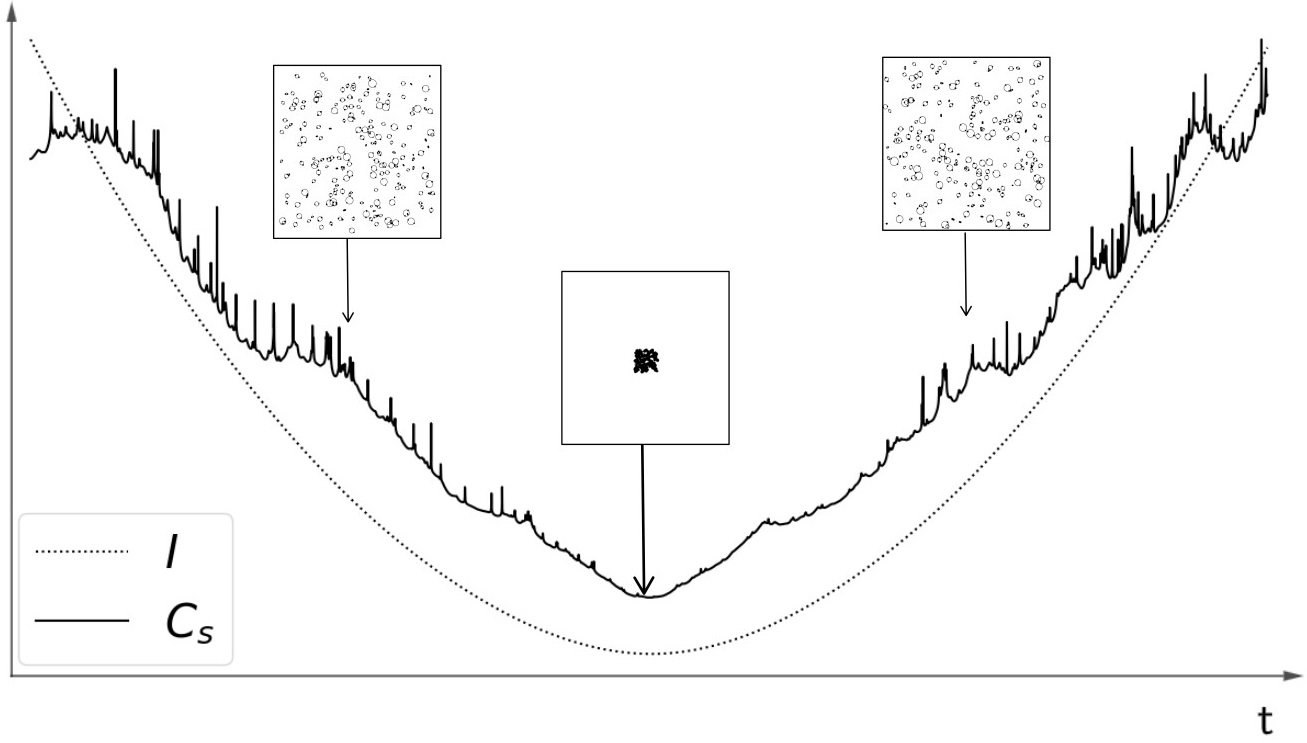
\includegraphics[width=0.5\linewidth]{tcc//img/complexidade.jpg}
    \caption{Visualização do espalhamento. O gráfico da complexidade corresponde a uma simulação de 100 corpos para $E=0$.}
    \label{fig:exemplo_espalhamento}
\end{figure}

% - A C_S É BOA POR DIVERSAS RAZÕES. ELA CARACTERIZA BEM TANTO A EVOLUÇÃO GERAL DO SISTEMA QUANTO O COMPORTAMENTO EM PEQUENA ESCALA. ELA CRESCER VARIANDO SIGNIFICA QUE A DISTANCIA ENTRE OS CORPOS FICA OSCILANDO.

% - SEGUNDO SAARI, PARA E = J = 0 O SISTEMA EVAPORA EM SUBSISTEMAS E CADA SUBSTISTEMA COMEÇA A CONVERGIR NO GERAL PARA CONSTANTES DE MOVIMENTO. QUANTO MAIS DIGITOS SAO CONSERVADOS EM UM SUBSISTEMA, MAIS ELE ESTÁ DISTANTE NA EVOLUÇÃO, ENTÃO A COMPLEXIDADE CARACTERIZA ISSO, A COMPLEXIDADE DO SISTEMA, O QUÃO ELE ESTÁ COMPLEXO. 

No caso em que $E=0$ e $\vet J = \vet 0$, \cite{Marchal1976} mostra que o sistema se divide em subsistemas (indexados por $\mathcal J$), e que cada subsistema, na medida em que se isola cada vez mais, desenvolve quantidade assintoticamente conservadas:
\begin{align*}
    E_{\mathcal J} (t) &= E_{\mathcal J} (\infty) + O(t^{-5/3}),\\
    \vet J_{\mathcal J} (t) &= \vet J_{\mathcal J} (\infty) + O(t^{-2/3}),\\
    \vet X_{\mathcal J} (t) / t &= \vet V_{\mathcal J} (\infty) + O(t^{-1/3}),
\end{align*}
onde $\vet X_{\mathcal J}$ é a distância do subsistema $\mathcal J$ ao centro de massas total do sistema e $\vet V_{\mathcal J} (\infty)$ é uma constante para a qual $\vet X_{\mathcal J}/t$ tende assintoticamente. Nessa situação, a complexidade caracteriza não apenas o distanciamento total entre os corpos, mas também as variações dentro dos subsistemas, como pode ser observado na figura \ref{fig:exemplo_espalhamento}, na qual $C_S$ cresce (indicando expansão do sistema) mas também varia (indicando as oscilações nos subsistemas).

% - ALEM DISSO, C_S É UM POTENCIAL DA FORMA DESEJADA, E UMA VEZ QUE R REMOVE A DEPENDENCIA DE ESCALA DE V_NEW, AS FORÇAS DERIVADAS DE C_S PODEM APENAS MUDAR A FORMA (SHAPE) DO SISTEMA, E NÃO O SEU TAMANHO. - LOG C_S TOMA O PAPEL DE POTENCIAL QUE ATRAI O SISTEMA TOWARDS MORE INHOMOGENEOUS SHAPES, E TEM MINIMOS E PONTOS DE SELA, MAS NAO MAXIMO GLOBAL.

\subsection{Equações de movimento no espaço de formas $S$}

Outro ponto para a complexidade como energia potencial do sistema é o fato de que $R$ remove a dependência da escala de $V$, então as forças derivadas de $C_S$ são capazes apenas de mudar a forma do sistema, e não o seu tamanho. A função $-\log C_S$ toma o papel de um potencial que leva o sistema para formas mais não-homogêneas.

% - COM ISSO EM MÃOS, AGORA DEFINIMOS AS NOVAS COORDENADAS E PODEMOS RE-ESCREVER O LOG R E OBTER UM HAMILTONIANO LEGAL MAS tau-DEPENDENTE. 

Com a decomposição da energia cinética e a nova energia potencial, agora é possível obter uma expressão para $\mathcal H$ em função de $\vet \sigma$ e $\vet \pi$. Isso é feito tomando em conta que
\begin{equation*}
    R^2 E - M^3 R C_S - \frac{1}{2} D^2 - \frac{1}{2} D_0^2 K_S = 0,
\end{equation*}
e então se $E = 0$ é possível obter uma expressão para $R$, e consequentemente para $\mathcal H$:
\begin{equation}\label{eq:hamiltoniano_tau_dependente}
    \mathcal H (\tau) = \log{(K_S + \tau^2)} - \log{C_S}.
\end{equation}

Para esse hamiltoniano $\tau$-dependente, obtemos um conjunto de equações de Hamilton também $\tau$-dependentes:
\begin{equation}
    \der{\vet \sigma_a}{\tau} = \dfrac{2 \vet \pi_a}{K_S + \tau^2},
    \quad
    \der{\vet \pi_a}{\tau} = \derpar{\log C_S}{\vet \sigma_a} - \dfrac{K_S}{K_S + \tau^2} \vet \sigma.
\end{equation}

% - PODEMOS ENTÃO INTRODUZIR LAMBDA = LOG TAU E DIVIDIR PI POR D, OQ FORNECE UM HAMILTONIANO AUTONOMO QUE DESCREVE METADE DO SISTEMA. POREM, AS EQUAÇÕES AGORA POSSUEM UMA FRICÇÃO NÃO CANONICA -OMEGA QUE ESPONTANEAMENTE DISSIPA O MOMENTO ADIMENSIONAL. ISSO JUNTO DO FATO DO POTENCIAL -LOGCS NAO TER MINIMO LOCAL EXPLICA POR QUE CS CRESCE SECULARMENTE (PORQUE É O OPOSTO DE UM POTENCIAL DE UM SISTEMA COM FRICÇÃO)
\subsection{A escala como fricção em $S$}

A dependência temporal de $\mathcal H$ pode ser eliminada através de uma mudança de coordenadas. Tomando $\lambda = \log \tau$ e definindo $\vet \omega_a = \vet \pi^a / \tau$ como um novo momento conjugado adimensional, obtemos um novo hamiltoniano $H_0$ dado por
\begin{equation}
    H_0 = \log\left(\sum_{a=1}^{N} \vet \omega^a \cdot \vet \omega^a + 1\right) - \log C_s,
\end{equation}
O custo dessa transformação é obter um conjunto não canônico de equações de movimento:
\begin{equation}
    \der{\vet \sigma_a}{\lambda} = \derpar{H_0}{\vet \omega_a},
    \quad
    \der{\vet \omega_a}{\lambda} = - \derpar{H_0}{\vet \sigma_a} - \vet \omega_a.
\end{equation}

O termo $\vet \omega_a$ na equação do momento é um tipo de  \textit{fricção sobre as equações}, indicando que existe dissipação. Dinamicamente, isso indica que o distanciamento dos subsistemas, refletido no problema original no aumento da escala, é refletido em $S$ por uma desaceleração na medida em que se aproxima do bordo da esfera unitária, ao ponto de, no limite, ter velocidade nula. Isso caracteriza uma assimetria sobre as trajetórias em $S$.

Por outro lado, o sistema com $H_0$ indica mais nitidamente o comportamento do sistema. Uma vez que o movimento é regido por um potencial $-\log C_S$ sujeito a fricção linear, $C_S$ deve crescer indefinidamente no problema com integrais primeiras nulas. Além disso, a dinâmica para $H_0$ tem um início delimitado, com um passado distante sendo o ponto-limite em que $D=0$. Isso reforça que $C_S$ possui um mínimo global, denominado \textit{Ponto de Janus}, a partir do qual o sistema pode evoluir em duas direções ($D > 0$ e $D < 0$), sendo cada direção orientada pelo crescimento de $C_S$. Dessa forma, $C_S$ caracteriza uma seta do tempo para o PNCG.

% - SETAS. DESCREVEMOS O PNCG COMO UM SISTEMA DINAMICO NO ESPAÇO DE FORMAS CUJO MOVIMENTO É REGIDO POR UM POTENCIAL -LOG CS SUJEITO A FRICÇÃO LINEAR. NESSE CASO, TEMOS UMA ORIENTAÇÃO PARA O SISTEMA: A DIREÇÃO EM QUE A ESTRUTURA, MEDIDA POR CS, CRESCE.
\subsection{Observações}

O caso em que $\vet J = 0$ mas $E > 0$, porém, é particularmente interessante, pois grande parte da teoria apresentada permanece válida. No lugar do $\mathcal H$ de \ref{eq:hamiltoniano_tau_dependente}, obtemos um hamiltoniano diferente:
\begin{equation*}
    \mathcal H = \log{\left[ C_S + \sqrt{C_S^2 + \frac{1}{2} \epsilon (K_S + \tau ^2)} \right]},
    \quad
    \epsilon = E D_0^2.
\end{equation*}
Nesse caso, o princípio de Mach-Poincaré falha, uma vez que é necessário especificar $\epsilon \tau^2$, mas a dinâmica continua invariante por escala e totalmente adimensional com uma variável monótona independente. No entanto, a evolução final fica mais firmemente estabelecida: o potencial é dependente do tempo e é idêntico a $C_S$ somente no instante inicial, apresentando um comportamento dissipativo com o tempo. Assintoticamente, o sistema congela.

% - QUESTÕES. AS EQUAÇÕES OBJETIVAS EM S MUDAM SE E E J NAO SAO NULOS. NESSE CASO O UNIVERSO CORRESPONDE NÃO APENAS A S MAS A ESTRUTURAS EXTERNAS. POREM, O CASO E = J = 0 BATE COM A ESTRUTURA BÁSICA DO CLOSED-SPACE VACUUM GR E PROVIDENCIA UM MODELO OK PRO UNIVERSO. ALEM DISSO, CS PODE PARECER UM CASAMENTO ARTIFICIAL SÓ PARA DAR ALGO ADIMENSIONAL, MAS O QUE É ARTIFICIAL É SEPARAR R DE V_NEW.
Outros valores para as integrais primeiras podem ser considerados. No entanto, se $E$ e $\vet J$ não são nulos as trajetórias não se resumem a $S$, mas dependem de outras estruturas externas. Uma vez que, como mencionado, o caso com integrais primeiras nulas quando estendido para a versão relativística da Dinâmica de Formas coincide com a Relatividade Geral, são valores razoáveis para se assumir como hipótese.

Outro ponto é sobre o processo de obtenção de $C_S$. Embora soe artificial a definição da complexidade como feita, $C_S$ é adimensional e caracteriza intrinsecamente a dinâmica do PNCG, sendo portanto um valor que de fato \textit{existe} para o problema. Por outro lado, separar a evolução do sistema entre $R$ e $V$, entre os corpos distantes e os corpos próximos, é o que se poderia chamar de artificial.

Assim, para além de um modelo interessante, a Dinâmica de Formas foi introduzida neste trabalho primeiro como motivação, e segundo como uma fonte de propriedades qualitativas do PNCG que podem ser visualizadas através de simulações numéricas. Na seção \ref{secao:simulacao_dinamica_de_formas} nós retomamos e aplicamos numericamente um pouco do que foi apresentado nesta seção.


% Nesse sentido, para $E \geq 0$, como $D$ é monótono este pode ser usado como uma medida de tempo $\tau = D/D_0$, onde $D_0 = D(t_0)$.

% \begin{figure}
%     \centering
%     \includegraphics[width=0.5\linewidth]{tcc//img/complexidade1000.png}
%     \caption{N=1000, h=0.04, e=0.04, [-10³, 10³], verlet, 464s + 451s}
%     \label{fig:enter-label}
% \end{figure}
% \begin{figure}
%     \centering
%     \includegraphics[width=0.5\linewidth]{tcc//img/complexidade_1000_energia_0.png}
%     \caption{Enter Caption}
%     \label{fig:enter-label}
% \end{figure}

% \begin{figure}
%     \centering
%     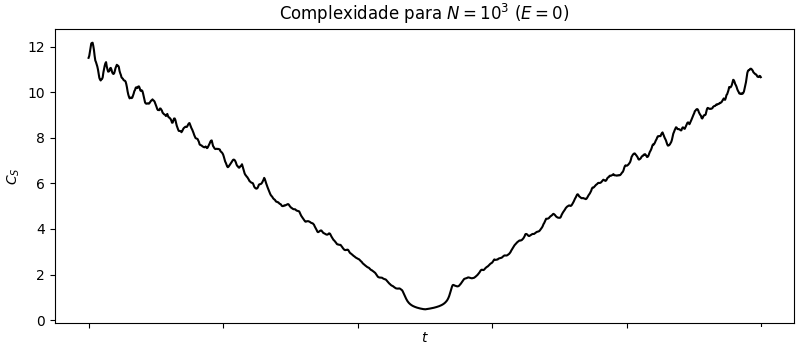
\includegraphics[width=0.5\linewidth]{tcc//img/complexidade_1000_nula.png}
%     \caption{Enter Caption}
%     \label{fig:enter-label}
% \end{figure}
\chapter{Métodos numéricos}\label{capitulo:metodos_numericos}

A integração numérica é o processo de aproximar o valor de uma integral numericamente com alguma margem de erro. Existe uma infinidade de formas de calcular essa aproximação, desde métodos baseados puramente em ferramentas básicas de cálculo até métodos baseados em teoria de variedades diferenciáveis e grupos de Lie.

Neste capítulo apresentamos uma pequena parte destes métodos, aplicando-os especificamente para a integração temporal, e contemplando principalmente o que foi utilizado nas simulações do PNCG. O capítulo começa com métodos tradicionais, baseados em cálculo de derivadas e geometria, principalmente para facilitar a habituação com os conceitos de integração numérica. Recomendamos \cite{alexandre_megiorin_roma_metodos_nodate} e \cite{Butcher2016-jx} para um estudo mais aprofundado.

Em seguida, entramos no ramo dos integradores simpléticos, aplicando numericamente os conceitos apresentados no capítulo \ref{capitulo:revisao_mecanica} a respeito da Mecânica Hamiltoniana. Em resumo, os integradores simpléticos são elaborados levando-se em conta não somente aspectos geométricos da função que está sendo integrada, mas também de todo o espaço que a contém. No caso, integramos sistemas hamiltonianos e portanto as propriedades do espaço de fases, como as integrais primeiras, são levadas em conta nos métodos através do conceito de \textit{simplectomorfismo}. A bibliografia principal utilizada e altamente recomendada é \cite{Hairer2006-oz} e \cite{Leimkuhler2005}.

Ao final, apresentamos um corretor numérico utilizado posteriormente à integração. O corretor se baseia nas integrais primeiras e aplica uma projeção via método de quadrados mínimos entre as hipersuperfícies no espaço de fases, fornecendo uma aproximação verossímil ao problema no sentido de que a estrutura simplética passa a ser conservada nas trajetórias ainda que não seja utilizado um integrador simplético.

Existem muitos outras formas de fazer a integração numérica. Em muitos contextos são utilizados métodos implícitos (explicados mais adiante), métodos com tamanho de passo variável, e até métodos voltados especificamente para o PNCG que preservam a energia e o momento angular com precisão de máquina, como \cite{Kotovych2002} propõem. Neste trabalho nos limitamos aos métodos explícitos tradicionais e aos simpléticos.

Por fim, os métodos foram testados com problemas-modelo escolhidos. Estes constam no Anexo \ref{apendice:problemas-modelo}.

% \begin{table}[]
%     \centering
%     \begin{tabular}{c|ccccccc}
%         $h$              & E. S. & Verlet & Ruth3 & Ruth4 & RK4 & RKN551 & RKN671  \\
%         \hline
%         $1/10$  & $1.129548$ & $1.904978$ & $3.567326$ & $3.398327$ &	$3.964893$ & $5.367215$ & $5.392546$ \\
%         $1/20$  & $1.057072$ & $1.974542$ & $3.659927$ & $3.840014$ &	$4.046272$ & $5.869322$ & $5.836890$ \\
%         $1/40$  & $1.021997$ & $1.993517$ & $3.540536$ & $3.959375$ &	$4.041771$ & $5.998531$ & $5.958402$ \\
%         $1/80$  & $1.008801$ & $1.998372$ & $3.361093$ & $3.989805$ &	$4.025951$ & $5.948801$ & $5.989673$ \\
%         $1/160$ & $1.003795$ & $1.999592$ & $3.208686$ & $3.997449$ &	$4.014280$ & $5.588236$ & $6.003132$ \\
%     \end{tabular}
%     \caption{Convergência dos métodos no problema modelo.}
%     \label{tab:my_label}
% \end{table}

% \begin{table}[]
%     \centering
%     \begin{tabular}{c|ccccc}
%         $h$              & E. E. & E. I. & RK22 & RK33 & RK44 \\
%         \hline
%         $1/40$   & $0.712071$ & $1.859924$ & $1.989241$ & $2.936490$ & $4.041771$ \\
%         $1/80$   & $0.827102$ & $1.283719$ & $2.003212$ & $2.965188$ & $4.025951$ \\
%         $1/160$  & $0.904085$ & $1.122329$ & $2.003873$ & $2.981701$ & $4.014280$ \\
%         $1/320$  & $0.949289$ & $1.057240$ & $2.002516$ & $2.990612$ & $4.008214$ \\
%         $1/640$  & $0.973898$ & $1.027730$ & $2.001404$ & $2.995243$ & $3.992159$ \\
%     \end{tabular}
%     \caption{Convergência dos métodos no problema modelo.}
%     \label{tab:my_label}
% \end{table}


%%%%%%%%%%%%%%%%%%%%%%%%%%%%%%%%%%%%%%%
%%% INTRODUÇÃO
%   Apresentar ideia dos métodos numéricos e a necessidade 
%   no caso do Problema de N-corpos. Falar brevemente dos 
%   tipos de métodos e o objetivo deste capítulo;
%%%%%%%%%%%%%%%%%%%%%%%%%%%%%%%%%%%%%%%
%%%%%%%%%%%%%%%%%%%%%%%%%%%%%%%%%%%%%%%%%%%%%%%%%%%%%%%%%%%%%%%%%
% > CONCEITOS BASICOS DE INTEGRACAO NUMERICA
%%%%%%%%%%%%%%%%%%%%%%%%%%%%%%%%%%%%%%%%%%%%%%%%%%%%%%%%%%%%%%%%%
\section{Conceitos básicos de integração numérica}

A ideia dos integradores numéricos é aproximar a solução exata de um problema de Cauchy em um intervalo $[a,b] \subseteq \R$, discretizando-o em um conjunto finito de $m+1$ pontos na forma
\begin{equation*}
    t_0 = a, \quad
    t_1 = t_0 + h_1 \quad
    \hdots \quad
    t_m = t_{m-1} + h_m = b,
\end{equation*}
onde cada $h_i \in \R$, $i = 1, ..., m$, é um \textit{passo de integração do instante $i$}. Neste trabalho, exceto quando explicitado o contrário, $h_i = h = (b-a)/m$, para todo $i$, então a discretização assume a forma
\begin{equation*}
    t_k = a + hk, \quad k = 1, 2, ..., m.
\end{equation*}

Com o intervalo discretizado, é possível obter uma diversidade de discretizações do problema em si. Assim, um problema do tipo
\begin{equation}\label{eq:problema_de_cauchy}
    \begin{cases}
        \der{}{t} y(t) = f(t,y(t)), \quad t \in [a,b], \\
        y(t_0) = y(a) = y_0,
    \end{cases}
\end{equation}
com $f:[a,b] \times \R^n \to \R^n$ e $y$ com condições suficientes para garantir existência e unicidade em $[a,b]$, pode ser discretizado na forma:
\begin{equation*}
    y(t_{k+1}) \approx y_{k+1} = \Phi_h(t_k, y_k), \quad k = 0, 1, ..., m-1,
\end{equation*}
onde $\Phi_h$ é chamado \textit{fluxo numérico} ou \textit{discreto}. Quando depender somente de $h$, $t_k$ e $y_k$, diremos que $\Phi_h$ é um \textit{método de passo único}; no caso contrário, será um \textit{método de passo múltiplo}.

Para cada instante da aproximação, podemos definir um \textit{erro local de discretização}.

\begin{definition}\label{def:erro_local_discretizacao}
    O \textbf{erro local de discretização} $\alpha_k$ do método numérico $\Phi_h$ em um instante discretizado $t_k \in [a,b]$ é dado por:
    \begin{equation*}
        \alpha_k := \dfrac{y(t_{k+1}) - \Phi_h(t_k, y(t_k))}{h}.
    \end{equation*}
\end{definition}

Nesse sentido, suponha que $\Phi_h$ é um método de passo único, ou seja, $\Phi_h(t_k,y_k) = y_k + h \tilde{\Phi}_h(t_k,y_k)$. Pensando na integração de Riemann, é intuitivo que quanto menor o tamanho de $h$, menor também será o erro. Porém, se $h \to 0$, uma vez que $t_k = h k + t_0$, teria-se que $t_k = t_0$ sempre. A saída para isso é fixar $t \in [a,b]$ e manter $hk = t - t_0$ fixo com $h \to 0$, o que significa que $k \to \infty$. Temos então para o erro local:
\begin{align*}
    \lim_{h \to 0} \alpha_k
    &= \lim_{h \to 0} \left[ \dfrac{y(t_{k+1}) - \Phi_h(t_k, y(t_k))}{h} \right] \\
    &= \lim_{h \to 0} \left[ \dfrac{y(t_k + h) - y(t_k)}{h} - \tilde{\Phi}_h(t_k, y_k) \right] \\
    &= f(t,y(t)) - \tilde{\Phi}_0(t,y(t)).
\end{align*}

Para um problema bem posto, espera-se de um método numérico então que o erro local deva ser cada vez menor, e que no limite seja zero. Nesse caso, dizemos que o método é \textit{consistente}.

\begin{definition}
    Dizemos que um integrador de passo único $\Phi_h(t_k,y_k) = y_k + h \tilde{\Phi}_h(t_k,y_k)$ é \textbf{consistente} se $\tilde{\Phi}_0(t,y) = f(t,y)$ ou, equivalentemente, $\lim_{h \to 0} \alpha_k = 0$, para $t \in [a,b]$ com $hk = t - t_0$ fixado.
\end{definition}

A consistência garante que, em alguma medida, a aproximação fornecida pelo método numérico (a partir de um valor exato e conhecido da trajetória) é próxima da solução exata do problema. Assim, também é possível atribuir à consistência uma \textit{ordem} da maneira que segue.

\begin{definition}
    Se existirem $C, h_0, q >0$ para quaisquer $h$ e $k$, tais que o erro local satisfaça:
    \begin{equation*}
        \max_k \norma{\alpha_k} \leq C h^q, \quad 0 < h \leq h_0,
    \end{equation*}
    então o método tem \textit{ordem de consistência} $q$ atrelada a norma $\norma{\cdot}$, que, a menos da explicitação do contrário, será a norma euclidiana usual.
    Nesse caso, um método consistente com ordem de consistência $q$ pode ser escrito da seguinte maneira:
    \begin{equation*}
        y(t_{k+1}) = \Phi_h(t_k, y_k) + O(h^q).
    \end{equation*}
\end{definition}

O que ocorre, porém, é que no geral se conhece somente o valor inicial do problema, e então define-se outra medida de erro, chamada \textit{erro global}. 

\begin{definition}
    O erro global $e_h(t_k)$ é o erro acumulado pelo método numérico até o instante discreto $t_k$:
    \begin{equation*}
        e_h (t_k) := e_k := y(t_k) - y_k.
    \end{equation*}
\end{definition}

O que se espera de um método minimamente utilizável é que seu erro global esteja ligado somente com o tamanho do passo $h$, de modo que 
\begin{equation}\label{eq:criterio_convergencia_1}
    \lim_{h \to 0} \dfrac{e_k}{h} = 0, \quad k = 0, 1, ..., m-1.
\end{equation}
para qualquer problema de Cauchy bem posto. 

\begin{definition}\label{def:convergencia}
    Um integrador $\Phi_h$ para o qual vale \ref{eq:criterio_convergencia_1} para qualquer problema de Cauchy bem posto é dito \textbf{convergente}, e dizemos que o integrador de passo único e explícito tem ordem de convergência $p$ se, e só se,
    \begin{equation*}
        e_h(t) = O(h^{p+1}).
    \end{equation*}
\end{definition}

A partir do erro global, é possível determinar condições suficientes para que um método de passo único explícito seja convergente. Supondo que $\tilde{\Phi}_h (t_k, \vet y_k) = \dfrac{1}{h} (\Phi_h (t_k, \vet y_k) - \vet y_k)$ satisfaça a condição de Lipschitz para $\vet y$, ou seja,
\begin{equation*}
    \norma{\tilde{\Phi}_h(t, \vet y_1) - \tilde{\Phi}_h(t, \vet y_2)}
    \leq
    L \norma{\vet y_1 - \vet y_2}
\end{equation*}
e que o erro de discretização local $\alpha_k$ seja limitado por $\alpha$, então \citep[29]{alexandre_megiorin_roma_metodos_nodate}
\begin{equation}
    \norma{e_k} \leq e^{k h L} \norma{e_0} + \dfrac{e^{k h L} - 1}{L} \alpha.
\end{equation}

Para o que interessa neste trabalho, $\norma{e_0} = 0$, então se um método explícito e de passo único é consistente com ordem $q$, ou seja, existe $C$ constante tal que $\alpha = C h^q$, então
\begin{equation*}
    \norma{e_k} \leq \dfrac{e^{k h L} - 1}{L} C h^q.
\end{equation*}
Dessa forma, o método também é convergente de ordem $q$.

Através do erro global, também é possível obter uma expansão em série de potências para uma aproximação numérica. Trataremos a questão para problemas de Cauchy em $\R$ por maior facilidade de exposição, mas todo o processo pode ser estendido para mais dimensões aplicando normas sobre os vetores.

\begin{theorem}\label{teorema:erro_global_expansao}\citep[30]{alexandre_megiorin_roma_metodos_nodate}
    Considere um problema de Cauchy com solução suficientemente diferenciável em um intervalo $[a,b]$ e uma aproximação $\eta(t,h)$ obtida através de um método de passo único
    \begin{equation*}
        \eta_{k+1} = \eta_k + h \tilde \Phi(t_k, \eta_k, h)
    \end{equation*}
    de ordem $p$ com tamanho de passo fixo $h = (t-t_0)/n$ para cada $t_0, t \in [a,b]$ e $n$ inteiro positivo. Nessas condições, $\eta(t,h)$ admite expansão em potências de $h$ da forma
    \begin{equation*}
        \eta(t,h) = y(t) + h^p e_p (t) + h^{p+1} e_{p+1} (t) + \hdots + h^N e_N(t) + h^{N+1} E_{N+1}(t,h).
    \end{equation*}
\end{theorem}

Do teorema \ref{teorema:erro_global_expansao} decorre que o erro de discretização global no instante $t$ pode ser escrito como
\begin{equation*}
    - e_h (t) = \eta (t,h) - y(t) = \sum_{j=p}^N h^j e_j(t) + h^{N+1} E_{N+1} (t,h).
\end{equation*}
Nesse sentido, para um $h$ suficientemente pequeno, temos uma aproximação razoável para o erro:
\begin{equation*}
    - e_h (t) = \eta (t, h) - y(t) \approx e_p (t) h^p.
\end{equation*}
Observe que a diferença entre aproximações com tamanho de passo $h$ e $h/2$ pode ser aproximado por
\begin{equation*}
    \eta (t, h) - \eta(t, h/2) \approx e_p(t) \left(\dfrac{h}{2}\right)^p (2^p - 1)
\end{equation*}
e logo
\begin{equation*}
    e_p (t) \left(\dfrac{h}{2}\right)^p \approx \dfrac{\eta (t, h) - \eta (t,h/2)}{2^p - 1}.
\end{equation*}
Isso fornece um valor aproximado para $e_{h/2}(t)$ se considerando um $h > 0$ suficientemente pequeno:
\begin{equation*}
    e_{h/2} (t) \approx - \dfrac{\eta(t,h) - \eta(t,h/2)}{2^p -  1}.
\end{equation*}

Todo esse processo supõe que o valor de $p$ é conhecido. No entanto, para fins práticos, é possível estimar $p$ realizando simulações com diferentes tamanhos de passo. Para um tamanho de passo $h$ de referência, considere $\eta (t, 2h)$, $\eta (t, h)$ e $\eta (t, h/2)$. Temos:
\begin{equation*}
    \left|\dfrac{\eta(t, 2h) - \eta(2,h)}{\eta(t, h) - \eta(t, h/2)}\right|
    \approx
    \left| \dfrac{e_{\tilde p}(t) (2^{\tilde p} - 1) h^{\tilde p}}{e_{\tilde p} (t) (1-2^{-\tilde p}) h^{\tilde p}} \right| = 2^{\tilde p},
\end{equation*}
então
\begin{equation}\label{eq:aproximacao_ordem}
    \tilde p \approx \log_2{\left| \dfrac{\eta(t, 2h) - \eta(2,h)}{\eta(t, h) - \eta(t, h/2)} \right|}.
\end{equation}
Para triplas de passos $(2h, h, h/2)$, $(h,h/2,h/4)$, ..., cada vez menores, a sequência $\tilde p_1, \tilde p_2, ...$ converge para $p$.

Para mais detalhes de integradores de passo único, o material de \cite{alexandre_megiorin_roma_metodos_nodate}, o qual foi consultado para esta seção, é bastante agregador. Para agora, com esses conceitos em mãos, já é possível começar a busca por integradores numéricos tradicionais, baseados somente em conceitos de cálculo e geometria analítica.

%%%%%%%%%%%%%%%%%%%%%%%%%%%%%%%%%%%%%%%
%%% METODOS TRADICIONAIS
%   Ideia e métodos de Euler;
%   Estabilidade e afins;
%   Exemplos de métodos:
%       Runge-Kutta 44;
%       Runge-Kutta-Fehlberg 45 (talvez);
%%%%%%%%%%%%%%%%%%%%%%%%%%%%%%%%%%%%%%%
%%%%%%%%%%%%%%%%%%%%%%%%%%%%%%%%%%%%%%%%%%%%%%%%%%%%%%%%%%%%%%%%%
% > METODOS TRADICIONAIS DE INTEGRACAO NUMERICA
%%%%%%%%%%%%%%%%%%%%%%%%%%%%%%%%%%%%%%%%%%%%%%%%%%%%%%%%%%%%%%%%%
\section{Métodos tradicionais de integração numérica}
\subsection{Integradores básicos de primeira ordem}

Considere o problema \ref{eq:problema_de_cauchy}. Uma primeira ideia para produzir métodos numéricos é utilizar da linearização fornecida pela primeira derivada temporal para, a partir de um instante $t_k$, aproximar a trajetória no instante $t_{k+1}$, o que naturalmente é possível para qualquer problema de Cauchy bem posto. Essa aproximação é chamada de \textit{método de Euler explícito}.

\begin{method}[Euler explícito]\label{metodo:euler_explicito}
    Para $h=(b-a)/m$ e $k = 0, 1, ..., m-1$, temos a aproximação:
    \begin{equation*}
        t_{k+1} = t_k + h, \quad
        y_{k+1} = y_k + h f (t_k, y_k) = \Phi_h(t_k, y_k).
    \end{equation*}
\end{method}

\begin{figure}[H]
    \centering
    \begin{tikzpicture}[x=1cm,y=1cm]\centering
    \draw[-latex] (-0.5,0)--(4,0); % eixo x
    \draw[-latex] (0,-0.5)--(0,4); % eixo y

    \draw[dashed] (0,1.2) node[left] {$y_0$}--(1,1.2)--(1,0) node[below] {$t_0$}; % y0 -- * -- t0
    \draw[dashed] (1,1.2)--(2,1.2)--(2,0) node[below] {$t_0+h$}; % * -- * -- t_1 = t0+h
    \draw[dashed] (0,2) node[left] {$y_1$}--(2,2)--(2,1.2); % y1 -- * -- t_1 = t0+h
    \draw[dashed] (0,3) node[left] {$y(t_1)$}--(2,3)--(2,2); % y(t1) -- * -- *

    % reta passando pelos pontos (t0, y0) e (t0+h,y1)
    \draw[thick, orange] (-0.2,0.24) -- (3,2.8);

    % a curva
    \draw[very thick, cyan] (-0.3,0.7) 
    to[out=50,in=210] (0,0.9) 
    to[out=30,in=218.66] (1,1.2) 
    to[out=38.66,in=260] (2,3)
    to[out=80,in=200] (2.5,3.5);

    % pontos pretos (bullet)
    \foreach \Point in {(1,1.2),(2,2),(2,3)}{
        \node at \Point {\textbullet};
    }
\end{tikzpicture}
    \caption{Visualização geométrica do método de Euler explícito, onde a curva é a solução exata e a reta é a solução aproximada.}
    \label{fig:euler_explicito_grafico}
\end{figure}

O método de Euler explícito é assim chamado pois fornece explicitamente a sua aproximação em função do instante e do passo anterior, como pode ser visualizado na figura \ref{fig:euler_explicito_grafico}. Uma outra forma de utilizar a primeira derivada é de maneira implícita, no que é chamado \textit{método de Euler implícito}.

\begin{method}[Euler implícito]\label{metodo:euler_implicito}
    Para $h=(b-a)/m$ e $k = 0, 1, ..., m-1$, temos a aproximação:
    \begin{equation*}
        t_{k+1} = t_k + h, \quad
        y_{k+1} = y_k + h f (t_{k+1}, y_{k+1}) = \Phi_h(t_{k+1}, y_{k+1}).
    \end{equation*}
\end{method}

Nesse caso, para avançar a solução no tempo é necessário não apenas aplicar uma fórmula, mas resolver um sistema algébrico de equações geralmente não-lineares no qual $y_{k+1}$ é a incógnita, o que não só exige mais processamento quando utilizado na prática como também pode acumular erros que estão além do método utilizado. Por exemplo, nesses casos é comum utilizar algum método de ponto fixo ou mesmo métodos de Newton ou Quasi-Newton, sendo que nos últimos casos é necessária a estimativa numérica de uma matriz jacobiana $n \times n$ e um certo número de iterações para garantir convergência, o que é custoso e, como todo método numérico, agrega com mais um erro acumulado. Por conta de tudo isso, os métodos numéricos implícitos não foram utilizados nas maiores simulações e não serão tratados neste trabalho. Ainda assim, tais métodos contam com certas vantagens que serão comentadas no decorrer do texto. Mais detalhes dos métodos implícitos e seu uso podem ser encontrados em \cite{Hairer2006-oz}.

Quanto à consistência e à convergência, os métodos propostos são consistentes com 1ª ordem de convergência, pois
\begin{align*}
    e_h(t_{k+1}) 
    &= y(t_{k+1}) - \Phi_h(t_k, \vet y(t_k)) \\
    &= \left(y(t_k) + h \dvet y(t_k) + \dfrac{h^2}{2!} \ddvet y(\xi)\right) - \left( \vet y(t_k) + h f(t_k, \vet y_k) \right) \\
    & = \dfrac{h^2}{2} \ddvet y(\xi),
    \quad
    \xi \in (t_k, t_{k+1}),
\end{align*}
o que pela definição \ref{def:convergencia} implica a ordem 1.

Para exemplificar, considere o problema-modelo \ref{probmodelo:lemniscata} aplicado nos métodos descritos com tamanhos de passo $1/20$, $1/40$, ..., $1/1280$. O resultado pode ser visualizado na tabela \ref{tab:euler_exp_imp_lemniscata}.

\begin{table}[]
    \centering
    \begin{tabular}{c|cc}
        $h$      & Explícito & Implícito   \\
        \hline
        $1/40$   & $0.712071$ & $1.859924$ \\
        $1/80$   & $0.827102$ & $1.283719$ \\
        $1/160$  & $0.904085$ & $1.122329$ \\
        $1/320$  & $0.949289$ & $1.057240$ \\
        $1/640$  & $0.973898$ & $1.027730$ \\
    \end{tabular}
    \caption{Convergência dos métodos de Euler explícito e implícito no problema-modelo \ref{probmodelo:lemniscata}.}
    \label{tab:euler_exp_imp_lemniscata}
\end{table}

Para a aplicação do método de Euler implícito foi utilizado o método de ponto fixo
\begin{equation*}
    \vet y_{k+1}^{[0]} = \vet y_k, \quad \vet y_{k+1}^{[i+1]} = \vet y_k + h f(t_{k+1}, \vet y_{k+1}^{[i]}),
\end{equation*}
para $i=1,...,Q$. Existem diversos critérios para a aplicação deste método \citep[325-335]{Hairer2006-oz}. Porém, como o método não foi de fato utilizado em mais nenhuma outra situação e não foi de nosso interesse neste momento trabalhar com os métodos implícitos no geral, $Q$ foi fixado para $Q=100$ e isso foi mais que suficiente para convergência.


%%%%%%%%%%%%%%%%%%%%%%%%%%%%%%%%%%%%%%%%%%%%%%%%%%%%%%%%%%%%%%%%%
% > METODOS DE RUNGE-KUTTA
%%%%%%%%%%%%%%%%%%%%%%%%%%%%%%%%%%%%%%%%%%%%%%%%%%%%%%%%%%%%%%%%%
\subsection{Métodos de Runge-Kutta}
Uma primeira ideia para obter métodos de ordem mais alta pode ser utilizar séries de Taylor, uma vez que o próprio método de Euler explícito pode ser encontrado via Taylor. O método resultante é como segue.

\begin{method}[Série de Taylor]\label{metodo:taylor}
    Suponha que $f$ do problema \ref{eq:problema_de_cauchy} é de ordem no mínimo $\continuo^q$, e seja $h$ um tamanho de passo fixo. Então
    \begin{equation*}
        \vet \Phi_h(t, \vet y) = y_k + h f(t, \vet y) + \dfrac{h^2}{2!} Df(y,\vet y) + \dfrac{h^3}{3!} D^2 f(t,\vet y) + \hdots + \dfrac{h^q}{q!} D^{q-1} f(t, \vet y),
    \end{equation*}
    onde $D = \derpar{}{t} + f \derpar{}{\vet y}$.
\end{method}

É possível verificar que tal método tem ordem $q$ \citep[42]{alexandre_megiorin_roma_metodos_nodate}. No entanto, tal método traz uma barreira no geral intransponível de maneira analítica para problemas práticos: é preciso encontrar as $q-1$ derivadas de $f$.

Os métodos de Runge-Kutta surgem nesse contexto, a partir da generalização do método de Euler para ordens mais altas, permitindo obter um método de passo único explícito, que concorda com o método \ref{metodo:taylor} para uma dada ordem $q$ e que substitui o cálculo das derivadas de $f$ por médias ponderadas e aplicações de $f$, ou \textit{estágios}, em pontos estratégicos.

\begin{method}[Runge-Kutta de $R$-estágios]\label{metodo:rk_r_estagios}
    Considere o problema \ref{eq:problema_de_cauchy} e tome um tamanho de passo $h$ fixo. Temos
    \begin{equation*}
        \Phi_h(t_k, \vet y_k) = \vet y_k + h \sum_{r=1}^{R} b_r \vet \kappa_r = \vet y_k + h \vet b^T \bm K,
        \quad \bm K = (\kappa_1, ..., \kappa_R)
    \end{equation*}
    onde
    \begin{align*}
        \vet \kappa_r (t,\vet y) &= f\left(t + h c_r, \vet y + h \sum_{j=1}^R a_{rj} \vet \kappa_j \right),
        \quad 1 \leq r \leq R.
    \end{align*}
\end{method}

Os parâmetros $a_{rj}$, $b_r$ e $c_r$ variam para cada método, mas para métodos explícitos sempre satisfazem as relações
\begin{equation}\label{eq:hipoteses_runge_kutta_explicito}
    \begin{aligned}
        \text{(i)} \quad & \sum_{r=1}^{R} b_r = 1, \\
        \text{(ii)} \quad & c_r = \sum_{j=1}^{r-1} a_{rj}, \quad 2 \leq r \leq R.
    \end{aligned}
\end{equation}

A condição (i) é suficiente e necessária para consistência, pois $h \to 0$ leva $\vet \kappa_r (t, \vet y) \to f (t, \vet y)$, então
\begin{equation*}
    \sum_{r=1}^{R} b_r \vet \kappa_r  = f(t,y) \sum_{r=1}^R b_r = f(t,\vet y).
\end{equation*}
Já (ii) garante a concordância com o método de Taylor, conforme \cite[45]{alexandre_megiorin_roma_metodos_nodate}.

Uma notação comum para representar as constantes $a_{rj}$, $b_r$ e $c_r$ é a Tabela de Butcher, dada pela seguinte forma:
\begin{table}
    \centering
    \begin{tabular}{c|c}
         $\vet c$ & $\bm A$\\
         \hline
                  & $\vet b$
    \end{tabular}
    \caption{Tabela de Butcher.}
\end{table}

Observe que o método de Euler explícito (método \ref{metodo:euler_explicito}) é um método de Runge-Kutta de ordem 1 com tabela
\begin{table}
    \centering
    \begin{tabular}{c|ccccc}
         $0$      & \\
         \hline
                  & 1
    \end{tabular}
    \quad
    \begin{tabular}{c|ccccc}
         $1$      & 1  \\
         \hline
                  & 1
    \end{tabular}
    \caption{Tabela de Butcher para os métodos de Euler explícito e implícito, respectivamente.}
\end{table}

Uma grande quantidade de métodos de Runge-Kutta é conhecida, com as mais diferentes ordens. Vale ressaltar também que a ordem de um método de Runge-Kutta é sempre menor ou igual ao número de estágios, ou seja, um método explícito de ordem $p$ tem uma quantidade de estágios $s \geq p$. Mais ainda, se $p \geq 5$, então $s > p$. No geral, parece existir uma tendência de que conforme $p$ aumenta, o valor mínimo de $s$ passa a ser $p + k_p$, para $k_p$ uma constante associada a $p$. Isso, porém, é ainda um problema não resolvido acerca dos métodos de Runge-Kutta \citep[187-196]{Butcher2016-jx}.

Apresentamos a seguir os métodos de ordem 2, 3 e 4, que são os métodos tradicionais mais frequentemente utilizados \citep[46-47]{alexandre_megiorin_roma_metodos_nodate}.

\begin{method}[Runge-Kutta de Segunda Ordem e Dois Estágios (RK22)]\label{metodo:rk22} 
    O método RK22 tem a seguinte Tabela de Butcher:
    \begin{table}[H]
        \centering
        \begin{tabular}{c|cccc}
             $0$      &       &      \\
             $1/2$    & $1/2$  &      \\
             \hline
                      & $0$ & $1$
        \end{tabular}
        \caption{Tabela de Butcher para o método RK22.}
    \end{table}
\end{method}

\begin{method}[Runge-Kutta de Terceira Ordem e Três Estágios (RK33)]\label{metodo:rk33} 
    O método RK33 tem a seguinte Tabela de Butcher:
    \begin{table}[H]
        \centering
        \begin{tabular}{c|cccc}
             $0$      &       &       &     \\
             $1/2$    & $1/2$ &       &     \\
             $1$      & $-1$   & $2$  &     \\
             \hline
                      & $1/6$ & $4/6$ & $1/6$
        \end{tabular}
        \caption{Tabela de Butcher para o método RK33.}
    \end{table}
\end{method}

\begin{method}[Runge-Kutta de Quarta Ordem e Quatro Estágios (RK44)]\label{metodo:rk44} 
    O método RK44 tem a seguinte Tabela de Butcher:
    \begin{table}[H]
        \centering
        \begin{tabular}{c|ccccc}
             $0$      &       &       &       &\\
             $1/2$    & $1/2$ &       &       &\\
             $1/2$    & $0$   & $1/2$ &       &\\
             $1$      & $0$   & $0$   & $1$   & \\
             \hline
                      & $1/6$ & $1/3$ & $1/3$ & $1/6$
        \end{tabular}
        \caption{Tabela de Butcher para o método RK44.}
    \end{table}
\end{method}

O mesmo método para depuração da ordem dos métodos (ver (\ref{eq:aproximacao_ordem})) pode ser aplicado para os métodos de Runge-Kutta no problema-modelo \ref{probmodelo:lemniscata}. O resultado consta na tabela \ref{tab:rk_lemniscata}.

\begin{table}[]
    \centering
    \begin{tabular}{c|ccc}
        $h$     & RK22 & RK33 & RK44 \\
        \hline
        $1/40$  & $1.989241$ & $2.936490$ & $4.041771$ \\
        $1/80$  & $2.003212$ & $2.965188$ & $4.025951$ \\
        $1/160$ & $2.003873$ & $2.981701$ & $4.014280$ \\
        $1/320$ & $2.002516$ & $2.990612$ & $4.008214$ \\
        $1/640$ & $2.001404$ & $2.995243$ & $3.992159$ \\
    \end{tabular}
    \caption{Convergência dos métodos RK22, RK33 e RK44 no problema-modelo \ref{probmodelo:lemniscata}}
    \label{tab:rk_lemniscata}
\end{table}


%%%%%%%%%%%%%%%%%%%%%%%%%%%%%%%%%%%%%%%%%%%%%%%%%%%%%%%%%%%%%%%%%
% > ESTABILIDADE DOS METODOS TRADICIONAIS
%%%%%%%%%%%%%%%%%%%%%%%%%%%%%%%%%%%%%%%%%%%%%%%%%%%%%%%%%%%%%%%%%
\subsection{Estabilidade dos integradores tradicionais}
Outra questão importante a se analisar sobre integradores numéricos é como se comportam em intervalos ilimitados, não apenas em intervalos limitados como feito até então. Para isso, é utilizado como problema modelo o problema de valor inicial mais simples possível:
\begin{equation}\label{eq:edo_problema_linear}
    \dvet y(t) = \bm M \vet y(t), \quad \vet y(t_0) = \vet y_0,
\end{equation}
sendo $\bm M$ uma matriz constante. O método de Euler explícito aplicado com um tamanho de passo $h$ assume a seguinte forma para o instante $t_k = t_0 + k h$:
\begin{equation}\label{eq:edo_linear_aproximacao}
    \vet y_k = (\bm I + h \bm M) \vet y_{k-1}
    \quad
    \therefore
    \quad
    \vet y_k = (\bm I + h \bm M)^k \vet y_0.   
\end{equation}
Além disso, da teoria de equações diferenciais, sabemos que a solução exata do problema (\ref{eq:edo_problema_linear}) é
\begin{equation}\label{eq:edo_linear_solucao}
    \vet y(t_k) = \exp{(k h \bm M)} \vet y_0.
\end{equation}

Considere uma mudança de base tal que $\vet y(t) = \bm A \vet z(t)$ e $\vet y_k = \bm A \vet z_k$, sendo $\bm A$ uma matriz constante e não singular. Temos então o problema nas novas coordenadas:
\begin{equation}
    \dvet z (t) = \bm A^{-1} \bm M \bm A \vet z(t) = \bm B \vet z(t),
    \quad
    \vet z(t_0) = \vet z_0,
\end{equation}
com solução exata
\begin{equation}
    \vet z(t_k) = \exp{(k h \bm B)} \vet z_0
\end{equation}
e solução aproximada
\begin{equation}
    \vet z_k = (\bm I + h \bm B)^k \vet z_0.
\end{equation}
Se a transformação escolhida é tal que $\bm B$ é a forma canônica de Jordan de $\bm M$, então para cada autovalor $\lambda$ tem-se uma equação diferencial da forma
\begin{equation}
    \dvet y(t) = \lambda \vet y(t),
\end{equation}
chamada \textbf{problema modelo} se $\RePart{\lambda} < 0$, com solução
\begin{equation}
    \vet y(t_k) = \exp{(k h \lambda}) \vet y_0.
\end{equation}
Assim, para o método de Euler explícito ser adequado é necessário que $(1+ h \lambda)^k$ seja uma aproximação aceitável para $\exp{(k h \lambda)}$, ou que no mínimo $(1+h \lambda)^k$ tenha comportamento limitado para $k \to \infty$ quando $\exp{(k h \lambda)}$ for limitado. Isso ocorre se e somente se $|1 + h \lambda| \leq 1$. Tomando $z = h \lambda$, a região complexa $|1+z| \leq 1$ é chamada de \textbf{região estável} para o método de Euler explícito, conforme figura \ref{fig:regiao_estabilidade_euler_explicito}.

\begin{figure}
    \centering
    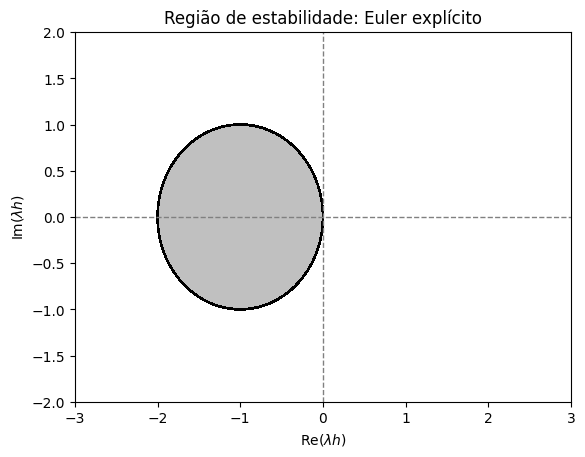
\includegraphics[width=0.5\linewidth]{tcc//img/regiao_estabilidade_euler.png}
    \caption{Região de estabilidade para o método de Euler explícito.}
    \label{fig:regiao_estabilidade_euler_explicito}
\end{figure}

\begin{definition}[Estabilidade de métodos numéricos]
    O problema de valor inicial
    \begin{equation*}
        \dot y(t) = \lambda y(t),
        \quad
        y(t_0) = y_0,
        \quad \RePart{\lambda} < 0
    \end{equation*}
    é chamado de \textbf{problema modelo}. Considere um método de passo único que aplicado ao problema modelo fornece a expressão
    \begin{equation*}
        y_{k+1} = \phi (\lambda h) y_k.
    \end{equation*}
    O conjunto $\Omega = \{\eta \in \mathbb{C} : |\phi(\eta)| < 1 \}$ é denominado \textbf{região de estabilidade absoluta} para $h>0$ fixado, $\phi(\lambda h)$ é chamado \textbf{fator de amplificação} e o intervalo $I_e = \Omega \cap \R$ é o \textbf{intervalo de estabilidade absoluta} do método. Um método \textbf{absolutamente estável} é também chamado de \textbf{A-estável}.
\end{definition}

Observando a região de estabilidade do método de Euler explícito, é fácil concluir que o método não é A-estável, uma vez que $|1+h \lambda| \leq 1$ somente se $h \leq - \RePart{\lambda} / |\lambda|$. Dizemos então que trata-se de um método \textbf{condicionalmente estável}.

Por outro lado, o método de Euler implícito (método \ref{metodo:euler_implicito}) tem uma comportamento diferente. Aplicando o mesmo processo anterior, obtemos a expressão
\begin{equation}
    \vet y_k = (1 - z)^{-1} \vet y_{k-1},
\end{equation}
e então sua região estável é $|1-z| \geq 1$, como na figura \ref{fig:regiao_estabilidade_euler_implicito}. Nesse caso, $\phi (\lambda h) = (1 - \lambda h)^{-1}$, então para qualquer $h > 0$ temos que $|\phi(\lambda h)| < 1$.

\begin{figure}
    \centering
    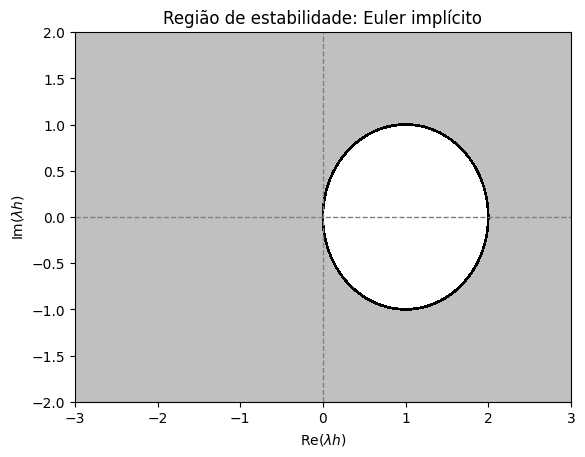
\includegraphics[width=0.5\linewidth]{tcc/img/regiao_estabilidade_euler_implicito.png}
    \caption{Região de estabilidade do método de Euler implícito}
    \label{fig:regiao_estabilidade_euler_implicito}
\end{figure}

É possível generalizar essa ideia para os métodos de Runge-Kutta. Tomando um método de ordem $s$ com tabela
\begin{table}
    \centering
    \begin{tabular}{c|c}
        $\vet c$ &  $\bm A$ \\
        \hline & $\vet b^T$
    \end{tabular}
\end{table}\\
temos para o problema modelo:
\begin{equation}
    \bm K = (\bm I - h \lambda \bm A)^{-1} \lambda \bm 1 y_0
    = (\bm I - z \bm A)^{-1} \lambda \bm 1 y_0,
\end{equation}
então
\begin{equation}\label{eq:ampliacao_rk_geral}
    y_1 
    = y_0 + h \vet b^T \bm K
    = [1 + z \vet b^T (\bm I - z \bm A)^{-1} \bm 1] y_0
    = R(z) y_0,
\end{equation}
sendo $R(\vet z)$ o fator de ampliação do método. Para o caso de métodos explícitos, a matriz $\bm A$ é triangular com diagonal nula, e portanto nilpotente com algum grau $k$. Através de uma expansão algébrica pode-se concluir que
\begin{equation}\label{eq:inversa_nilpotentes}
    (\bm I - z \bm A) = \bm I + \sum_{j=1}^{k-1} z^j \bm A^k.
\end{equation}
Substituindo (\ref{eq:inversa_nilpotentes}) em (\ref{eq:ampliacao_rk_geral}),
\begin{align*}
    R(z) 
    &= 1 + z \vet b^T (\bm I + \sum_{j=1}^{k-1} z^j \bm A^j)\bm 1 \\
    &= 1 + z \vet b^T \bm I \bm 1 + \vet b^T \sum_{j=1}^{k-1} z^{j+1} \bm A^j \bm 1.
\end{align*}
A partir de (\ref{eq:hipoteses_runge_kutta_explicito}), temos por (i) que $\vet b^T \bm I \bm 1 = \sum_{j=1}^s b_j = 1$. Temos então que
\begin{equation}
    R(z) = 1 + z + \sum_{j=1}^{k-1} z^{j+1} \bm A^j \bm 1.
\end{equation}
No caso dos métodos explícitos em que $p=s$, temos os seguintes fatores:
\begin{equation}
    R (z) = \begin{cases}
    1 + z, & p = 1, \\
    1 + z + \frac{1}{2} z^2, & p = 2, \\
    1 + z + \frac{1}{2} z^2 + \frac{1}{6} z^3, & p = 3, \\
    1 + z + \frac{1}{2} z^2 + \frac{1}{6} z^3 + \frac{1}{24} z^4, & p = 4.
    \end{cases}
\end{equation}
A região de estabilidade absoluta desses métodos pode ser vista na figura \ref{fig:regiao_estabilidade_rk_explicitos}, sendo o interior de cada curva fechada.

\begin{figure}
    \centering
    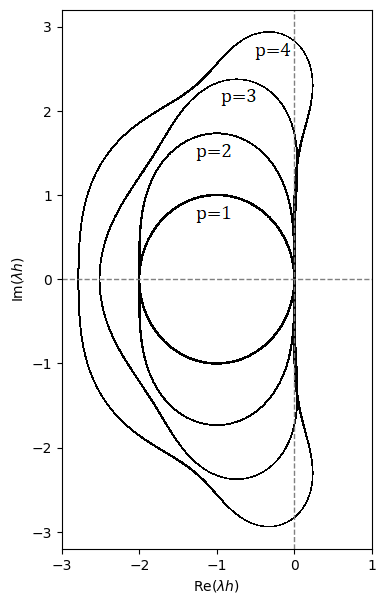
\includegraphics[width=0.35\linewidth]{tcc//img/regiao_estabilidade_rk.png}
    \caption{Região de estabilidade dos métodos de Runge-Kutta de ordens e estágios $p = 1, 2, 3$ e $4$.}
    \label{fig:regiao_estabilidade_rk_explicitos}
\end{figure}

Uma vez que as regiões de estabilidade são fechadas pois o fator é polinomial, os métodos de Runge-Kutta explícitos não são A-estáveis. Porém, da mesma forma que no caso dos métodos de Euler explícito e implícito, é possível obter A-estabilidade utilizando métodos implícitos. 
\begin{table}[H]
    \centering

    \begin{tabular}{c|cc}
        $\frac{1}{2} - \frac{\sqrt 3}{6}$ & $1/4$ & $\frac{1}{4} - \frac{\sqrt 3}{6}$ \\
        $\frac{1}{2} + \frac{\sqrt 3}{6}$ & $\frac{1}{4} + \frac{\sqrt 3}{6}$ & $1/4$ \\
        \hline & $1/2$ & $1/2$
    \end{tabular}
    
    \caption{Método de Runge-Kutta implícito de quarta ordem e dois estágios. \citep[99]{Butcher2016-jx}}.
    \label{tab:exemplo_metodo_runge_kutta_implicito}
\end{table}

Por exemplo, considere o método de quarta ordem da tabela \ref{tab:exemplo_metodo_runge_kutta_implicito}. Seu fator de amplificação é
\begin{equation*}
    R(z) = \dfrac{1 + \frac{z}{2} + \frac{z^2}{12}}{1 - \frac{z}{2} + \frac{z^2}{12}}.
\end{equation*}
Observe que $|R(z)| \leq 1$ somente se $\RePart{z} \leq 0$, e uma vez que $z = \lambda h$ com $\RePart{\lambda} < 0$, qualquer valor de $h$ garante estabilidade para o método, sendo então A-estável.

Apesar da maior facilidade para obter métodos implícitos de altas ordens e estáveis, a necessidade de utilizar métodos iterativos para resolver o sistema de equações pode não compensar computacionalmente tais ganhos qualitativos. Ainda assim, os métodos de Runge-Kutta implícitos são utilizados em diversas aplicações, inclusive porque todas as versões simpléticas dos métodos RK são necessariamente implícitas (veja o Teorema \ref{teorema:rk_simpletico}).

De toda forma, a A-estabilidade, por definição, se aplica para problemas lineares, o que não é o caso da grande maioria de aplicações práticas dos integradores numéricos. No entanto, muitos sistemas podem ser aproximados localmente por sua linearização, sendo então possível aplicar os resultados de estabilidade para obter tamanhos de passo adequados.

No problema de N-corpos, utilizar o método de Euler implícito não apresentou nenhuma vantagem. No entanto, ainda é possível observar algumas anomalias esperadas para cada método simulando, por exemplo, o problema-modelo \ref{probmodelo:lemniscata}. Na figura \ref{fig:lemniscata_euler_exp_imp_distancia} é possível observar a diferença na divergência entre os dois métodos quando comparados a um método simplético de alta ordem. Enquanto o método de Euler explícito apresenta um afastamento de órbita mais prolongado, o método de Euler implícito apresenta afastamentos mais breves.

\begin{figure}
    \centering
    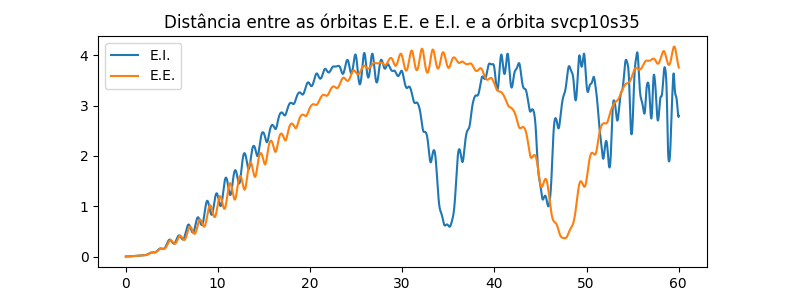
\includegraphics[width=0.75\linewidth]{tcc//img/lemniscata_euler_exp_imp_svcp10s35.png}
    \caption{Distância no espaço de fases entre as soluções numéricas do problema-modelo \ref{probmodelo:lemniscata} com métodos de Euler explícito e implícito e o método svcp10s35 com $h=10^{-3}$ no intervalo $[0,60]$.}
    \label{fig:lemniscata_euler_exp_imp_distancia}
\end{figure}

Um motivo para isso pode ser observado na figura \ref{fig:lemniscata_euler_exp_imp}. Uma vez que $E_0 - E$ decresce no método de Euler explícito, a energia total está aumentando, o que significa que a energia cinética está aumentando (ou que a potencial está diminuindo). Isso leva a um relaxamento do período e com aproximações mais violentas, e portanto ao menos uma partícula deve ser ejetada do sistema em sua evolução.

Já no caso implícito, $E_0-E$ cresce, logo a energia total está diminuindo, então a energia potencial está aumentando (ou a energia cinética está diminuindo). Isso implica no encolhimento do período, e como o PNCG pode conter colisões o sistema fica numericamente instável.

Na prática, o método de Euler explícito ``erra para mais'', expandindo a trajetória, enquanto o método de Euler implícito ``erra para menos'', contraindo a trajetória.

\begin{figure}
        \centering
        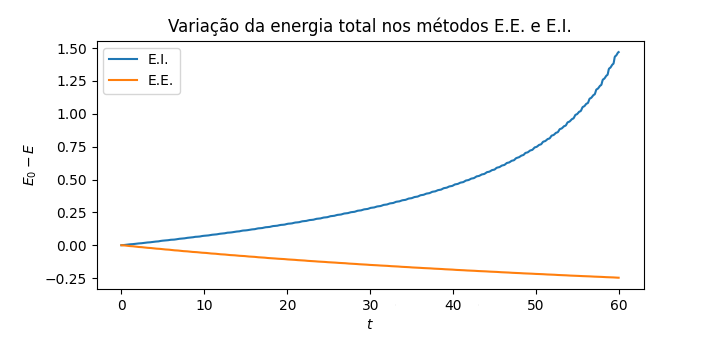
\includegraphics[width=0.7\linewidth]{tcc//img/lemniscata_euler_exp_imp.png}
        \caption{Variação (com sinal) da energia total em simulações do problema-modelo \ref{probmodelo:lemniscata} via métodos de Euler explícito e implícito e com $h=10^{-3}$ no intervalo $[0,60]$.}
        \label{fig:lemniscata_euler_exp_imp}
\end{figure}

%%%%%%%%%%%%%%%%%%%%%%%%%%%%%%%%%%%%%%%
%%% METODOS SIMPLÉTICOS
%   Ideia inicial dos métodos;
%   Estabilidade e afins;
%   Exemplos de métodos:
%       Euler Simplético (1a Ordem);
%       Velocity-Verlet (2a Ordem);
%       Ruth3 e Ruth4 (3a e 4a Ordem);
%       RKN551 e RKN671 (5a e 6a Ordem);
%       SVCP8S15 e SVCP10S35 (8a e 10a Ordem).
%   Comparacao numerica com os métodos tradicionais;
%%%%%%%%%%%%%%%%%%%%%%%%%%%%%%%%%%%%%%%
% IDEIA INICIAL:
%   Ideia inicial dos métodos;
%   Propriedades
%   Exemplos de métodos:
%       Euler Simplético (1a Ordem);
%       Velocity-Verlet (2a Ordem);
%       Ruth3 e Ruth4 (3a e 4a Ordem);
%       RKN551 e RKN671 (5a e 6a Ordem);
%       SVCP8S15 e SVCP10S35 (8a e 10a Ordem).
%   Comparacao numerica com os métodos tradicionais;

\section{Integradores simpléticos}\label{secao:integradores_simpleticos}
Como apresentado brevemente na introdução deste capítulo, os métodos simpléticos se baseiam na estrutura do espaço de fases, e não apenas na função que está sendo integrada. Nesse sentido, tais métodos são construídos de modo a preservarem a estrutura simplética dos problemas hamiltonianos, conservando o volume da solução e consequentemente conservando as integrais primeiras também.

Essas diferenças na forma e objetivo de construir os integradores entre os métodos tradicionais e os simpléticos têm implicações importantes sobre os resultados. Os métodos tradicionais são construídos tendo-se em vista uma estabilidade assintótica do sistema, imbuindo dissipações na solução numérica que distorcem as trajetórias de sistemas hamiltonianos, ainda que sejam aplicados integradores tradicionais de alta ordem, como exemplificado ao final da seção anterior. Isso não ocorre com integradores simpléticos, como apresentamos a seguir.

Para esta seção, no lugar de considerar um problema de Cauchy qualquer, tomaremos aqueles que podem ser escritos através das equações de Hamilton:
\begin{equation}\label{eq:pvi_hamilton}
    \dvet z(t) = \bm \Omega \nabla_{\vet z} H(\vet z),
    \quad
    \vet z(0) = \vet z_0,
    \quad
    \vet z(t) = (\vet q(t), \vet p(t)),
    \quad
    \bm \Omega = \begin{bmatrix}
        \bm 0 & \bm I \\ - \bm I & \bm 0
    \end{bmatrix}.
\end{equation}

Como já apresentado no capítulo \ref{capitulo:revisao_mecanica}, o fluxo do problema (\ref{eq:pvi_hamilton}) é \textit{simplético}, ou seja, conserva o volume no espaço de fases. Em particular, isso significa que conserva também as integrais primeiras do sistema. A proposta dos \textit{integradores simpléticos} é fornecer uma aplicação simplética $\vet \Phi_h$ tal que
\begin{equation*}
    \vet z_1 = \vet \Phi_h(\vet z_0).
\end{equation*}
Ademais, conforme o teorema \ref{teorema:simpleticidade_matricial}, um critério para $\vet \Phi_h$ ser simplética é ser tal que
\begin{equation*}
    D \Phi_h \bm \Omega D \Phi_h^T = \bm \Omega.
\end{equation*}


\subsection{Obtenção de métodos via separação}
Quando a função hamiltoniana é separável, ou seja, $H(\vet q, \vet p) = T(\vet p) + V(\vet q)$, é possível obter métodos explícitos a partir do que segue. Tomando como hamiltoniano primeiramente apenas $T$ e em seguida apenas $V$, temos os dois problemas de valor inicial respectivos:
\begin{equation}
    \begin{cases}
        \dvet q = \nabla_{\vet p} T(\vet p) = \dfrac{1}{m} \vet p, \\
        \dvet p = \vet 0,
    \end{cases},
    \quad
    \begin{cases}
        \dvet q = \vet 0, \\
        \dvet p = - \nabla_{\vet q} V(\vet q) = F(\vet q).
    \end{cases}   
\end{equation}
Em ambos os casos, podemos obter o fluxo de maneira explícita, uma vez que uma das coordenadas está constante:
\begin{equation}
    \vet \Phi_{\tau, T} (\vet z) = \begin{bmatrix}
        \vet q + \tau \vet p/m \\ \vet p
    \end{bmatrix},
    \quad
    \vet \Phi_{\tau, V} (\vet z) = \begin{bmatrix}
        \vet q \\ \vet p + \tau \vet F(\vet q)
    \end{bmatrix}.
\end{equation}
Se tomamos a aplicação composta $\vet \Phi_{\tau} := \vet \Phi_{\tau, T} \circ \vet \Phi_{\tau, V}$, obtemos um primeiro método com semblante familiar.

\begin{method}[Euler Simplético (ou semi-implícito)]\label{metodo:euler_simpletico}
    Para um tamanho de passo $h$ fixo em um intervalo discretizado para um problema de valor inicial hamiltoniano separável, temos a aproximação:
    \begin{equation}
        \vet q_{k+1} = \vet q_k + h \dfrac{\vet p_{k+1}}{m},
        \quad
        \vet p_{k+1} = \vet p_k + h \vet F(\vet q_k).
    \end{equation}
\end{method}

Da mesma forma que os métodos de Euler explícito e implícito (métodos \ref{metodo:euler_explicito} e \ref{metodo:euler_implicito}, respectivamente), o método de Euler simplético tem ordem 1 \citep[189]{Hairer2006-oz}. No entanto, trata-se de um método simplético, pois vale o critério matricial (Teorema \ref{teorema:simpleticidade_matricial}):
\begin{equation*}
    D \vet \Phi_h = \begin{bmatrix}
        1 + \dfrac{h^2}{m} \nabla_{\vet q} \vet F(\vet q) & \dfrac{h}{m} \\
        h \nabla_{\vet q} \vet F(\vet q) & 1
    \end{bmatrix}
    \quad
    \Longrightarrow
    \quad
    D \vet \Phi_h \bm \Omega D \vet \Phi_h^T = \begin{bmatrix}
        \vet 0 & \bm I \\ - \bm I & \vet 0
    \end{bmatrix}
    = \bm \Omega.
\end{equation*}

A diferença entre os métodos pode ser observada aplicando-os no problema-modelo \ref{probmodelo:lemniscata}, como na figura \ref{fig:var_energia_rk22_rk33_rk44_es}. Veja que embora todos os métodos de Runge-Kutta (com ordem maior que 1) comecem com uma variação menor de energia que o método de Euler simplético (com ordem 1), a variação do segundo é relativamente preservada, enquanto que a dos métodos RK escalona. No caso do RK44, embora a precisão seja mantida por mais tempo para $h=0.05$, um tamanho de passo $h=0.15$ permite visualizar melhor o erro na energia escalonando.

\begin{figure}
    \centering
    \begin{subfigure}{.5\textwidth}
      \centering
      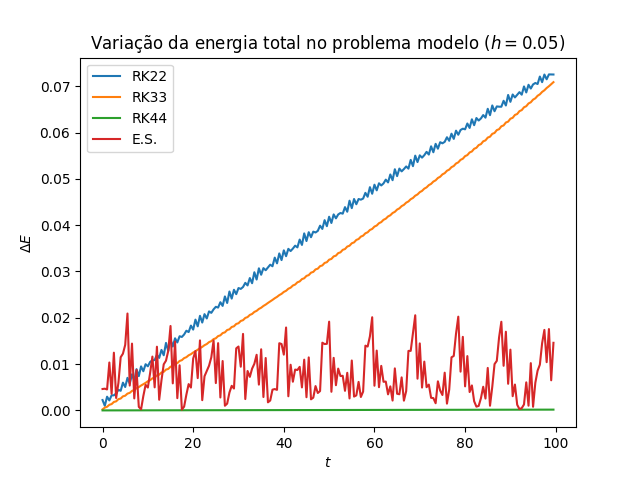
\includegraphics[width=\linewidth]{tcc/img/var_energia_rk22_rk33_rk44_es.png}
      \caption{Intervalo $[0,100]$ e $h=0.05$.}
      \label{fig:var_energia_rk22_rk33_rk44_es_a}
    \end{subfigure}%
    \begin{subfigure}{.5\textwidth}
      \centering
      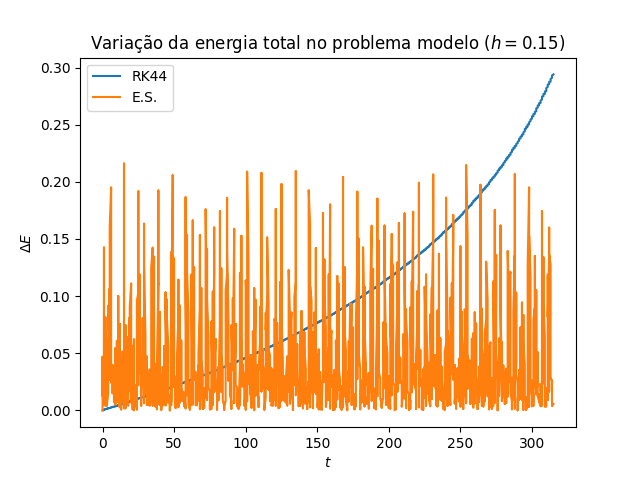
\includegraphics[width=\linewidth]{tcc/img/var_energia_rk44_es.png}
      \caption{Intervalo $[0,300]$ e $h=0.15$.}
      \label{fig:var_energia_rk22_rk33_rk44_es_b}
    \end{subfigure}
    \caption{Variação da energia total na simulação do problema-modelo \ref{probmodelo:lemniscata} com os métodos RK22, RK33, RK44 e Euler Simplético (E.S.)}
    \label{fig:var_energia_rk22_rk33_rk44_es}
\end{figure}

A ideia de composição também pode ser aplicada para obter métodos com ordem mais alta. Tomando constantes de peso (isto é, que somam 1) $c_1, ..., c_s$ e $d_1, ..., d_s$, tomamos a composição
\begin{equation*}
    \vet \Phi_h = \vet \Phi_{d_s h, V} \circ \vet \Phi_{c_s h, T} \circ \hdots \circ \vet \Phi_{d_1 h, V} \circ \vet \Phi_{c_1 h, T}.
\end{equation*}
Conforme \cite[145-146]{Leimkuhler2005}, métodos $\vet \Phi_h$ com esta forma são consistentes e, além disso, se os coeficientes são simétricos ($c_i = c_{s+1-i}$ e $d_i = d_{s+1-i}$), então o método tem no mínimo ordem 2.

\begin{method}[Velocity-Verlet]\label{metodo:velocity-verlet}
    Tomando os coeficientes $d_1=d_2=1/2$, $c_1 = 0$ e $c_2=1$, obtemos um método consistente, simétrico, explícito, simplético e de segunda ordem dado por
    \begin{align*}
        \vet q_{k+1} &= \vet q_k + h \dfrac{\vet p_k}{m} + \dfrac{h^2}{2 m} \vet F(\vet q_k), 
        \\
        \vet p_{k+1} &= \vet p_k + \dfrac{h}{2} (\vet F(\vet q) + \vet F(\vet q_{k+1})).
    \end{align*}
\end{method}

\begin{theorem}
    O método Velocity-Verlet é simplético.
\end{theorem}
\begin{Proof}
    Seja $\vet \Phi_h (\vet q, \vet p) = (\vet Q (\vet q, \vet p), \vet P(\vet q, \vet p))$. Então:
    \begin{align*}
        \derpar{\vet Q}{\vet q} &= 1 + \dfrac{1}{2} \dfrac{h^2}{m} \derpar{\vet F}{\vet q}, 
        &\quad
        \derpar{\vet Q}{\vet p} &= \dfrac{h}{m}, 
        \\
        \derpar{\vet P}{\vet q} &= \dfrac{h}{2} \derpar{\vet F}{\vet q} \left(1 + \derpar{\vet Q}{\vet q}\right),
        &\quad
        \derpar{\vet P}{\vet p} &= \derpar{\vet Q}{\vet q}.
    \end{align*}
    Nesse caso, a condição do teorema \ref{teorema:simpleticidade_matricial} é facilmente verificada:
    \begin{equation*}
        \derpar{\vet Q}{\vet q} \derpar{\vet P}{\vet p} - \derpar{\vet Q}{\vet p} \derpar{\vet P}{\vet q} 
        = \left(\derpar{\vet Q}{\vet q}\right)^2 - \left(\derpar{\vet Q}{\vet q} - 1\right) \left(1 + \derpar{\vet Q}{\vet q}\right) = 1.
    \end{equation*}
\end{Proof}

Outros dois métodos de ordens 3 e 4 foram propostos, respectivamente, por \cite{Ruth1983} e por \cite{Forest1990}.

\begin{method}[Ruth 3]\label{metodo:ruth3}
    Um método simplético de 3ª ordem é obtido através dos coeficientes
    \begin{align*}
        c_1 = 1,    & \quad & c_2 = -2/3, & \quad & c_3 = 2/3, \\
        d_1 = -1/24 & \quad & d_2 = 3/4,  & \quad & d_3 = 7/24.
    \end{align*}
\end{method}

\begin{method}[Ruth 4]\label{metodo:ruth4}
    Um método simplético de 4ª ordem é obtido através dos coeficientes
    \begin{align*}
        c_1 = c_4 = \dfrac{1}{2(2-2^{1/3})}, & \quad & c_2 = c_3 = \dfrac{1-2^{1/3}}{2(2-2^{1/3})}, \\
        d_1 = d_3 = \dfrac{1}{2-2^{1/3}}, & \quad & d_2 = - \dfrac{2^{1/3}}{2-2^{1/3}}, \quad d_4 = 0.
    \end{align*}
\end{method}


\subsection{Métodos via composição de integradores de segunda ordem}
Seguindo nessa linha, \cite{Yoshida1990} observa que uma forma eficiente de obter métodos de alta ordem para problemas com funções hamiltonianas separáveis é através da composição de métodos simétricos de segunda ordem. A facilidade vem dos termos ímpares da expansão de Taylor se anularem, o que simplifica as condições de ordem do método, e procurar por métodos de ordem par é conveniente uma vez que os métodos simétricos sempre têm ordem par e são reversíveis no tempo \citep[147]{Leimkuhler2005}. Vale ressaltar que a composição de simplectomorfismos é também simplectomorfa, o que significa que compôr métodos de Verlet, por exemplo, com uma boa escolha de pesos, fornece integradores simpléticos, simétricos, consistentes e de alta ordem. Nesse caso, as aplicações compostas $\vet \Psi_h$ têm a forma
\begin{equation*}
    \vet \Psi_h = \vet \Phi_{\gamma_s h} \circ \hdots \circ \vet \Phi_{\gamma_2 h} \circ \Phi_{\gamma_1 h},
\end{equation*}
onde $\vet \Phi_{\gamma_i h}$ é o método de Verlet (\ref{metodo:velocity-verlet}) com tamanho de passo $\gamma_i h$, para $i=1,2,...,s$. Dois métodos deste tipo foram implementados no programa final, com ordens 8 e 10.

\begin{method}[svcp8s15]\label{metodo:svcp8s15}\citep[157]{Hairer2006-oz}
    Um método Stormer-Verlet Composto de 8ª ordem e 15 estágios (svc8s15) é obtido através dos coeficientes:
    \begin{center}
        \begin{tabular}{ccccr}        
        $\gamma_1$ &$=$& $\gamma_{15}$ &$=$& $0.74167036435061295344822780$ \\
        $\gamma_2$ &$=$& $\gamma_{14}$ &$=$& $-0.40910082580003159399730010$ \\
        $\gamma_3$ &$=$& $\gamma_{13}$ &$=$& $0.19075471029623837995387626$ \\
        $\gamma_4$ &$=$& $\gamma_{12}$ &$=$& $-0.57386247111608226665638773$ \\
        $\gamma_5$ &$=$& $\gamma_{11}$ &$=$& $0.29906418130365592384446354$ \\
        $\gamma_6$ &$=$& $\gamma_{10}$ &$=$& $0.33462491824529818378495798$ \\
        $\gamma_7$ &$=$& $\gamma_{9}$  &$=$& $0.31529309239676659663205666$ \\
                   &   & $\gamma_{8}$  &$=$& $-0.79688793935291635401978884$ \\
        \end{tabular}
    \end{center}
\end{method}

\begin{method}[svcp10s35]\label{metodo:svcp10s35}\citep[158]{Hairer2006-oz}
    Um método Stormer-Verlet Composto de 10ª ordem e 35 estágios (svc8s15) é obtido através dos coeficientes:
    \begin{center}
        \begin{tabular}{ccccr}        
        $\gamma_1$  &$=$& $\gamma_{35}$ &$=$& $ 0.07879572252168641926390768$ \\
        $\gamma_2$  &$=$& $\gamma_{34}$ &$=$& $ 0.31309610341510852776481247$ \\
        $\gamma_3$  &$=$& $\gamma_{33}$ &$=$& $ 0.02791838323507806610952027$ \\
        $\gamma_4$  &$=$& $\gamma_{32}$ &$=$& $-0.22959284159390709415121340$ \\
        $\gamma_5$  &$=$& $\gamma_{31}$ &$=$& $ 0.13096206107716486317465686$ \\
        $\gamma_6$  &$=$& $\gamma_{30}$ &$=$& $-0.26973340565451071434460973$ \\
        $\gamma_7$  &$=$& $\gamma_{29}$ &$=$& $ 0.07497334315589143566613711$ \\
        $\gamma_8$  &$=$& $\gamma_{28}$ &$=$& $ 0.11199342399981020488957508$ \\
        $\gamma_9$  &$=$& $\gamma_{27}$ &$=$& $ 0.36613344954622675119314812$ \\
        $\gamma_{10}$ &$=$& $\gamma_{26}$ &$=$& $-0.39910563013603589787862981$ \\
        $\gamma_{11}$ &$=$& $\gamma_{25}$ &$=$& $ 0.10308739852747107731580277$ \\
        $\gamma_{12}$ &$=$& $\gamma_{24}$ &$=$& $ 0.41143087395589023782070412$ \\
        $\gamma_{13}$ &$=$& $\gamma_{23}$ &$=$& $-0.00486636058313526176219566$ \\
        $\gamma_{14}$ &$=$& $\gamma_{22}$ &$=$& $-0.39203335370863990644808194$ \\
        $\gamma_{15}$ &$=$& $\gamma_{21}$ &$=$& $ 0.05194250296244964703718290$ \\
        $\gamma_{16}$ &$=$& $\gamma_{20}$ &$=$& $ 0.05066509075992449633587434$ \\
        $\gamma_{17}$ &$=$& $\gamma_{19}$ &$=$& $ 0.04967437063972987905456880$ \\
                    &   & $\gamma_{18}$ &$=$& $ 0.04931773575959453791768001$ \\
        \end{tabular}
    \end{center}
\end{method}

Apesar da relativa facilidade de obter métodos simpléticos através de composição de métodos de primeira e de segunda ordem, é fácil ver pelos métodos \ref{metodo:svcp8s15} e \ref{metodo:svcp10s35} que é necessária uma quantidade de estágios muito maior do que a ordem do método, o que torna a usabilidade dos métodos cada vez mais desafiadora. Porém, existem muitos outros métodos simpléticos e que não são baseados em composição. Dois tipos bastante comuns são os métodos de Runge-Kutta Simpléticos e os métodos de Runge-Kutta-Nyström.

\subsection{Métodos de Runge-Kutta Simpléticos e de Runge-Kutta-Nyström}
Para obter um método de Runge-Kutta simplético basta adicionar uma restrição (além das já apresentadas anteriormente) sobre o método \ref{metodo:rk_r_estagios}.

\begin{theorem}\label{teorema:rk_simpletico}
    Se os coeficientes de um método de Runge-Kutta de $R$ estágios são tais que
    \begin{equation*}
        b_i a_{ij} + b_j a_{ji} - b_i b_j = 0, \quad i, j = 1, ..., R, 
    \end{equation*}
    então trata-se de um método simplético.
\end{theorem}

A demonstração do teorema pode ser encontrada em \cite[152-154]{Leimkuhler2005}. O importante neste momento é que decorre do teorema que para $i=j$ temos
\begin{equation*}
    2 a_{ii} = b_i, \quad \forall i = 1, 2, ..., R.
\end{equation*}
Uma vez que o vetor $\vet b$ não é nulo, isso significa que a matriz de coeficientes $\bm A$ tem diagonal não-nula, e portanto não é possível obter um integrador de Runge-Kutta simplético que seja explícito. Tendo em vista as já mencionadas dificuldades de se trabalhar computacionalmente com métodos implícitos, nenhum método de Runge-Kutta simplético foi testado neste trabalho.

Já os métodos de Runge-Kutta-Nyström (RKN) são voltados especificamente para problemas de valor inicial do tipo
\begin{equation*}
    \ddvet x = g(t, \vet x, \dvet x),
\end{equation*}
então são aplicáveis para grande parte dos problemas de mecânica hamiltoniana, como o PNCG. O método geral é dado pelo que segue.

\begin{method}[Runge-Kutta-Nyström de $s$ estágios]\citep[41]{Hairer2006-oz}
    Um método RKN de $s$ estágios para um sistema hamiltoniano separável em $T$ e $V$ é dado por
    \begin{align*}
        \vet y_i & = \vet q_k + c_i h \dfrac{\vet p_k}{m} + h^2 \sum_{j=1}^{s} a_{ij} \dfrac{\vet F(\vet y_i)}{m}, \quad i = 1, 2, ..., s, \\
        \vet q_{k+1} &= \vet q_k + h \dfrac{\vet p_k}{m} + h^2 \sum_{i=1}^{s} b_i \dfrac{\vet F(\vet y_i)}{m}, \\
        \vet p_{k+1} &= \vet p_k + h \sum_{i=1}^{s} B_i \vet F(\vet y_i),
    \end{align*}
    para constantes $\bm A, \vet b, \vet c$ e $B_1, ..., B_s$.
\end{method}

Da mesma forma que para os métodos de Runge-Kutta, um método RKN é explícito se $a_{ij} = 0$ para $j \geq i$. Porém, existem critérios para que um método RKN explícito seja simplético \citep[376]{Okunbor1994}:
\begin{align}
    b_i &= B_i (1-c_i), &\quad 1 \leq i \leq s, \\
    a_{ij} &= B_j(c_i - c_j), &\quad j < i.
\end{align}
Dessa forma, foi possível testar métodos de Runge-Kutta-Nyström simpléticos e explícitos. Os escolhidos para teste constam em \cite{Okunbor1994} e são como segue. O número 1 sufixado ao nome dos métodos indica que, em referência às tabelas 1 e 2 de Okunbor e Skeel, tratam-se do método 1. O método RKN551 foi escolhido entre os 4 sem critérios, e o RKN671 foi escolhido por ter o menor resíduo entre os apresentados pelos autores.

\begin{method}[RKN551]\label{metodo:rkn551}
    Um método RKN de 5ª ordem e 5 estágios simplético e explícito é dado pelos seguintes coeficientes:
    \begin{table}[H]
        \centering
        \begin{tabular}{r|r}
            \multicolumn{1}{c}{$B_i$} & \multicolumn{1}{c}{$c_i$} \\
            \hline
            -1.67080892327314312060 &  0.69491389107017931259 \\ 
             1.22143909230997538270 &  0.63707199676998338411 \\ 
             0.08849515813253908125 & -0.02055756998211598005 \\ 
             0.95997088013770159876 &  0.79586189634575355001 \\ 
             0.40090379269297793385 &  0.30116624272377778837 \\
             \hline
        \end{tabular}
    \end{table}
\end{method}

\begin{method}[RKN671]\label{metodo:rkn671}
    Um método RKN de 6ª ordem e 7 estágios simplético e explícito é dado pelos seguintes coeficientes:
    \begin{table}[H]
        \centering
        \begin{tabular}{lr}
            \hline
            $B_4$           &  0.26987577187133640373 \\ 
            $B_5 = B_3$     &  0.92161977504885189358 \\ 
            $B_6 = B_2$     &  0.13118241020105280626 \\ 
            $B_7 = B_1$     & -0.68774007118557290171 \\ 
            $c_4$           &  0.50000000000000000000 \\ 
            $c_5 = 1 - c_3$ &  0.06520862987680341024 \\ 
            $c_6 = 1 - c_2$ &  0.65373769483744778901 \\ 
            $c_7 = 1 - c_1$ &  0.05586607811787376572 \\ 
            \hline
        \end{tabular}
    \end{table}
\end{method}

\subsection{Comparações entre os métodos apresentados}
A mesma ideia de verificação de ordem para os métodos tradicionais pode ser aplicada para os métodos simpléticos, como é apresentado na tabela \ref{tab:convergencia_metodos_simpleticos}. Os integradores com ordem maior que 6 geram resultados muito parecidos mesmo para os valores de $h$ relativamente grandes utilizados na tabela e mesmo quando se utiliza precisão de 128 \textit{bits}, então não pudemos verificar sua precisão com este método.

\begin{table}[]
    \centering
    \begin{tabular}{c|ccccccc}
        $h$     & E. S. & Verlet & Ruth3 & Ruth4 & RKN551 & RKN671  \\
        \hline
        $1/10$  & $1.129548$ & $1.904978$ & $3.567326$ & $3.398327$ & $5.367215$ & $5.392546$ \\
        $1/20$  & $1.057072$ & $1.974542$ & $3.659927$ & $3.840014$ & $5.869322$ & $5.836890$ \\
        $1/40$  & $1.021997$ & $1.993517$ & $3.540536$ & $3.959375$ & $5.998531$ & $5.958402$ \\
        $1/80$  & $1.008801$ & $1.998372$ & $3.361093$ & $3.989805$ & $5.948801$ & $5.989673$ \\
        $1/160$ & $1.003795$ & $1.999592$ & $3.208686$ & $3.997449$ & $5.588236$ & $6.003132$ \\
    \end{tabular}
    \caption{Convergência dos métodos no problema modelo \ref{probmodelo:lemniscata}.}
    \label{tab:convergencia_metodos_simpleticos}
\end{table}

Vale também observar a diferença na conservação da energia entre cada método simplético, pois métodos de ordem maior conservam a energia também em maior ordem. Aplicando o problema-modelo \ref{probmodelo:lemniscata} para cada método apresentado, obtemos a figura \ref{fig:var_energia_simpleticos}.

\begin{figure}
    \centering
    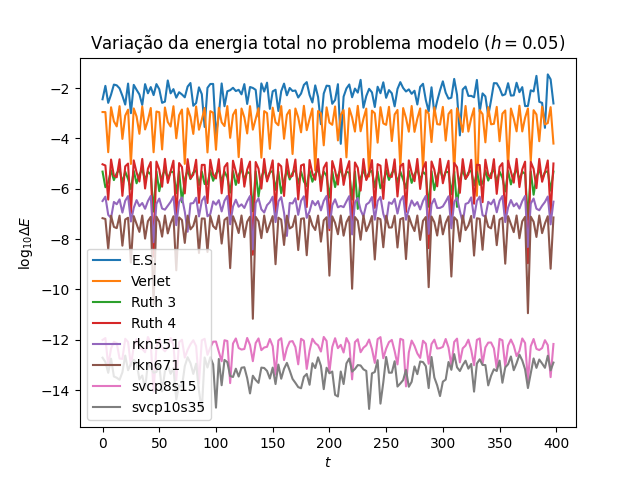
\includegraphics[width=0.7\linewidth]{tcc//img/var_energia_simpleticos.png}
    \caption{Variação da energia total para os métodos simpléticos apresentados. O problema-modelo \ref{probmodelo:lemniscata} foi integrado no intervalo $[0,400]$ com tamanho de passo $h=0.05$.}
    \label{fig:var_energia_simpleticos}
\end{figure}

Um ponto importante sobre os métodos simpléticos é que, como já dito, estes conservam não apenas a energia total, mas todas as integrais primeiras. Porém, a energia total é calculada através das velocidades e das distâncias entre os corpos, e corpos muito próximos geram instabilidade numérica no sentido de facilitarem o aparecimento de erros de ponto flutuante, enquanto as outras quantidades conservadas baseiam-se somente em operações lineares ou vetoriais diretas, sem a possibilidade de singularidades. A implicação prática disso é que as outras integrais primeiras são muito melhor conservadas que a energia total, como pode ser observado na figura \ref{fig:var_integrais_es_iau25}, na qual as outras integrais primeiras de um problema de 25 corpos possuem erro abaixo de $10^{-11}$. Dessa forma, é coerente analisar erros numéricos focando-se principalmente na energia.

\begin{figure}
    \centering
    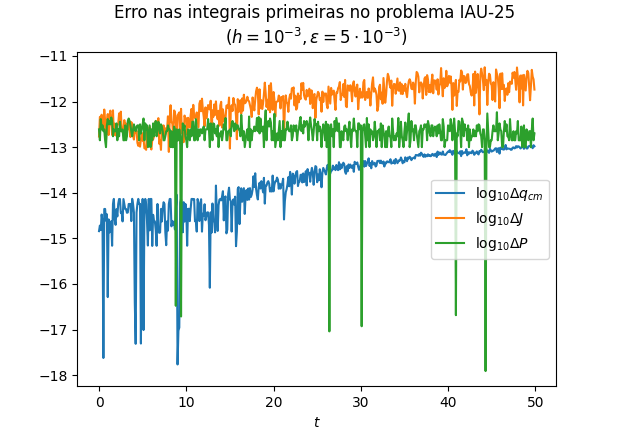
\includegraphics[width=0.5\linewidth]{tcc//img/var_integrais_es_iau25.png}
    \caption{Variação das integrais primeiras do PNCG na simulação do problema IAU-25 (\ref{probmodelo:iau25}) via método de Euler Simplético com tamanho de passo $h=10^{-3}$ e amortecimento $\epsilon=10^{-3}$. Aqui $\Delta f = |\norma{f} - \norma{f_0}|$.}
    \label{fig:var_integrais_es_iau25}
\end{figure}

%%%%%%%%%%%%%%%%%%%%%%%%%%%%%%%%%%%%%%%
%%% CORRETOR NUMÉRICO
%   Falar sobre o corretor numerico e exemplos de sua
%   aplicacao em problemas grandes e pequenos, alem do
%   custo computacional e da eficiencia.
%%%%%%%%%%%%%%%%%%%%%%%%%%%%%%%%%%%%%%%
\section{Corretor numérico}\label{secao:corretor_numerico}

Uma alternativa (ou complemento) ao uso de integradores simpléticos é utilizar integradores tradicionais e aplicar algum tipo de correção a cada passo, de modo a garantir que a solução aproximada conserve as integrais primeiras. O método apresentado nesta seção tem esse propósito, e, embora aqui tenha sido desenvolvido intuitivamente, este foi proposto inicialmente por \cite{Nacozy1972} e posteriormente analisado por \cite{Shampine1986}.

Sejam $\vet z = (\vet q, \vet p)$ um vetor no espaço de fases para um problema de $N$ partículas (não necessariamente o PNCG) e $\vet z_0 = (\vet q_0, \vet p_0)$ o valor inicial de um Problema de Cauchy conservativo
\begin{equation*}
    \dvet z (t) = F(t,\vet z(t)), \quad \vet z(t_0) = \vet z_0,
\end{equation*}
com $F$ suave. Seja também $\vet \Psi (\vet z) = (\psi_1(\vet z), ..., \psi_k(\vet z))$ um conjunto de $k$ integrais primeiras para o problema, sendo $\vet \Psi_0 = \vet \Psi(\vet z_0)$.

Tome um instante $t \in I$, sendo $I$ o intervalo maximal do problema, e considere a solução exata $\vet z^* = \vet z(t)$ e a solução aproximada $\tilde{\vet z}$, obtida através de um integrador numérico qualquer. Espera-se de uma boa simulação conservativa que $\vet z$ seja solução de
\begin{equation}\label{eq:problema_otimizacao_corretor}
    \begin{aligned}
        \min \quad & \norma{\tilde{\vet z} - \vet z^*} \\
        \text{s. a} \quad & \psi_i (\vet z^*) = \psi_i (\vet z_0) \\
        &  i = 1, ..., k.
    \end{aligned}
\end{equation}
Como o que se tem é $\tilde{\vet z}$, podemos analisar em função de $\vet z^*$.

\begin{figure}
    \centering
    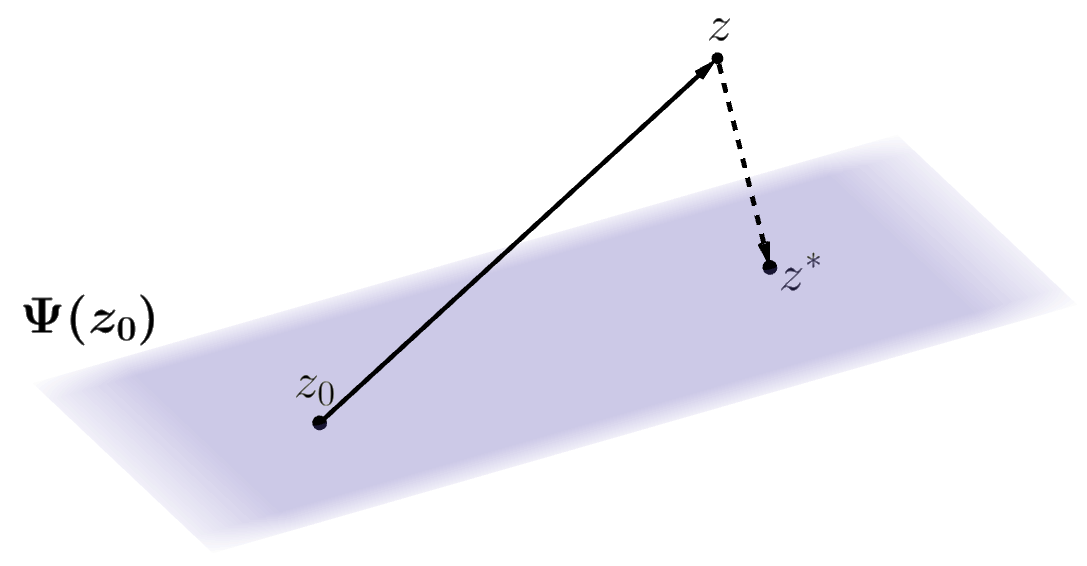
\includegraphics[width=0.5\linewidth]{tcc//img/corretor_visualizacao.png}
    \caption{Representação visual do corretor numérico.}
    \label{fig:corretor_visualizacao}
\end{figure}

Tome uma função $f(\vet x) = \frac{1}{2} \norma{\tilde{\vet z} - \vet x}^2$, cujo problema de otimização é equivalente a (\ref{eq:problema_otimizacao_corretor}). O processo se torna o método de quadrados mínimos. Tome $\vet y$ um candidato a mínimo do problema. As condições necessárias de otimização para o problema implicam que nesse caso \citep{Friedlander1994}:
\begin{equation}\label{eq:corretor_equacao_1}
    \nabla f(\vet y) = \tilde{\vet z} - \vet y
    = \sum_{i=1}^k \alpha_i \nabla \psi_i (\vet y) = D \vet \Psi (\vet y)^T \vet \alpha, 
    \quad \vet \alpha = (\alpha_1, ..., \alpha_k),
\end{equation}
onde $D \vet \Psi (\vet y)$ é a matriz jacobiana do campo vetorial de integrais primeiras e $\vet \alpha$ é o vetor de multiplicadores de Lagrange. Observe que a função objetivo $f$ é uma função convexa, e logo a condição necessária é também suficiente para o problema. Por Taylor, tem-se que
\begin{equation*}
    \vet \Psi (\tilde{\vet z}) \approx \vet \Psi (\vet y) + D \vet \Psi(\vet y) (\tilde{\vet z} - \vet y),
\end{equation*}
o que pela equação (\ref{eq:corretor_equacao_1}) pode ser escrito como:
\begin{equation}\label{eq:corretor_equacao_2}
    D \vet \Psi(\vet y) D \vet \Psi(\vet y)^T \vet \alpha 
    \approx
    \vet \Psi (\tilde{\vet z}) - \vet \Psi(\vet y)
    = 
    \vet \Psi (\tilde{\vet z}) - \vet \Psi(\vet z_0).
\end{equation}

Resolvendo (\ref{eq:corretor_equacao_2}) obtém-se os multiplicadores de Lagrange, que podem ser substituídos em (\ref{eq:corretor_equacao_1}):
\begin{equation*}
    \vet y = \tilde{\vet z} - D \vet \Psi(\vet y)^T \vet \alpha \approx \vet z^*.
\end{equation*}

Dessa forma, ainda que seja utilizado um método tradicional, é possível obter uma solução que preserve \textit{razoavelmente} as integrais primeiras. Essa \textit{razoabilidade} está ligada com o tamanho de passo $h$ escolhido da maneira como segue.

Considere um problema local no instante $t_n$ dado por
\begin{equation*}
    \dvet u (t) = F(t, \vet u(t)), \quad \vet u(t_n) = \vet z_n^*,
\end{equation*}
onde $\vet z_n$ é uma aproximação para o problema original no instante $t_n$ que satisfaz as integrais primeiras. Um tamanho de passo $h$ está relacionado a um erro local $\tau$ de modo que
\begin{equation*}
    \norma{u(t_{n+1}) - \vet z_{n+1}} \leq \tau.
\end{equation*}
Tomando uma aproximação corrigida $\vet z_{n+1}^*$, observe que
\begin{align*}
    \norma{\vet z(t_{n+1}) - \vet z_{n+1}^*} 
    & = \norma{\vet z(t_{n+1}) - \vet u(t_{n+1}) + \vet u(t_{n+1}) - \vet z_{n+1} + \vet z_{n+1} - \vet z_{n+1}^*} \\
    & \leq \norma{\vet z(t_{n+1}) - \vet u(t_{n+1})} + \norma{\vet u(t_{n+1}) - \vet z_{n+1}} + \norma{\vet z_{n+1} - \vet z_{n+1}^*} \\
    & \leq \zeta_h + \tau + \mu,
\end{align*}
onde $\zeta_h$ limita a norma de $\vet z(t_{n+1}) - \vet u(t_{n+1})$ e $\mu = \norma{\vet z_{n+1} - \vet z_{n+1}^*}$. A constante $\zeta_h$ é garantida por $f$ ser Lipschitz com constante $L$:
\begin{equation*}
    \norma{\vet z(t_{n+1}) - \vet u(t_{n+1})} \leq e^{h L} \norma{\vet z(t_n) - \vet z_n^*} = \zeta_h.
\end{equation*}
Quanto à $\mu$, se garantida sua existência como constante, então aplicar a correção sobre uma aproximação com erro $\tau$ possui um erro de discretização equivalente a não aplicar a correção sobre uma aproximação de erro $\tau + \mu$. 

Observe que $\vet u(t)$ satisfaz as integrais primeiras, pois seu valor inicial $\vet z_n^*$ as satisfaz. Em particular $\vet u(t_{n+1}) = \vet z_{n+1}^*$ satisfaz, e logo a correção é tal que $\mu = \tau$, o que significa que aplicá-la sobre uma aproximação de ordem $p$ fornece uma aproximação corrigida também de ordem $p$. Dessa forma, o corretor preserva a ordem do integrador.

Quanto à aplicação computacional, algumas questões merecem ser tratadas, e constam na seção \ref{secao:uso_do_corretor}.
\chapter{Implementação e aplicações}\label{capitulo:simulacao}

%%%%%%%%%%%%%%%%%%%%%%%%%%%%%%%%%%%%%%%
%%% INTRODUÇÃO / CONTEXTUALIZAÇÃO
%   Este sera um capitulo de aplicação. Falar brevemente de 
%   como serao feitos os testes e mais abertamente o que se 
%   quer aqui.
%%%%%%%%%%%%%%%%%%%%%%%%%%%%%%%%%%%%%%%
% * CONTEXTUALIZACAO E OBJETIVOS
%
%   Este sera um capitulo de aplicação. Falar brevemente de como serao
%   feitos os testes e mais abertamente o que se quer aqui.
%

O objetivo deste último capítulo é a aplicação da teoria apresentada. Começando pela implementação computacional, discutimos a escolha da linguagem de programação Fortran e a estrutura do programa final. Passamos então para as questões de valores iniciais, apresentando o método utilizado para condicionar as integrais primeiras.

A questão das colisões vem em seguida, pois existem outras formas computacionais de lidar com singularidades e aproximações intensas no PNCG além da inclusão de colisões perfeitamente elásticas.

Algumas questões sobre o corretor numérico apresentado na seção \ref{secao:corretor_numerico} também precisam ser discutidas, como o seu uso e seu custo de computação associado. Além disso, este envolve a resolução de um sistema de equações (para mais de uma integral primeira em consideração), então foi necessário escolher um método de resolução adequado.

Por fim, apresentamos algumas simulações de muitos corpos e com condições iniciais específicas para testar os resultados da Dinâmica de Formas enunciados na seção \ref{secao:dinamica_de_formas}.

Todas as simulações e testes realizados neste trabalho foram aplicados em um computador de mesa (não dedicado) com processador \textit{Intel Core i5 CPU 760 @ 2.80GHz} e com 16 GB de RAM.

% Como já explicitado, neste trabalho são consideradas os sistemas puramente gravitacionais e conservativos, além de pontuais, ou seja, cada corpo é um ponto individual. As simulações de grande porte utilizadas na astronomia e na cosmologia no geral consideram, no lugar de pontos de massa, funções de densidade $\rho$ e um campo gravitacional $\nabla \phi$, de modo que o potencial fica dado por uma equação de Poisson
% \begin{equation*}
%     \Delta \phi = - 4 \pi G \rho.
% \end{equation*}
% O campo é então discretizado através de métodos numéricos voltados para equações diferenciais parciais, e neste ponto é feita a integração numérica temporal. Isto é necessário por uma série de razões práticas, como a implementação de gases, galáxias e afins, indo bem além dos objetivos deste trabalho. [TALVEZ COLOCAR ISSO NA INTRODUÇÃO DO TRABALHO, E NÃO AQUI]

% Sendo assim, existe neste trabalho a necessidade de calcular direta e rapidamente expressões não-lineares com ordem quadrática, como o potencial gravitacional, sem o uso de aproximações como o algoritmo de Barnes-Hut [TALVEZ FALAR MELHOR SOBRE TAMBÉM, SÓ PRA NÃO FICAR JOGADO]. Isso levou à escolha do Fortran como linguagem de programação para as simulações, e suas particularidades serão melhor exploradas adiante.

%%%%%%%%%%%%%%%%%%%%%%%%%%%%%%%%%%%%%%%
%%% FERRAMENTAS
%   Defender a escolha do Fortran e apresentar informacoes
%   basicas: compilador, bibliotecas, etc.
%   Falar sobre a estrutura de dados, a forma de armazenamento,
%   a análise. 
%   Falar especificamente sobre a aplicacao no PNC, como a
%   paralelizacao, (SE ROLAR GPU TB), e especificadas do
%   codigo para o problema em questao.
%   Apresentar dificuldades.
%   Disponibilizar código.
%%%%%%%%%%%%%%%%%%%%%%%%%%%%%%%%%%%%%%%
% * FERRAMENTAS E CÓDIGO
%   
%   Defender a escolha do Fortran e apresentar informacoes
%   basicas: compilador, bibliotecas, etc.
%   Falar sobre a estrutura de dados, a forma de armazenamento,
%   a análise. 
%   Falar especificamente sobre a aplicacao no PNC, como a
%   paralelizacao, (SE ROLAR GPU TB), e especificadas do
%   codigo para o problema em questao.
%   Apresentar dificuldades.
%   Disponibilizar código.
\section{Ferramentas}

%%%%%%%%%%%%%%%%%%%%%%%%%%%%%%%%%%%%%
%%% ESCOLHA DA LINGUAGEM
%%%%%%%%%%%%%%%%%%%%%%%%%%%%%%%%%%%%%
\subsection{Escolha da linguagem de programação}
Como dito brevemente, a necessidade de muitas operações computacionalmente custosas com agilidade exigiu a escolha de uma linguagem de programação que fosse potente por natureza. 

Linguagens como o Python possuem excelentes bibliotecas voltadas para a computação científica, como o \textit{NumPy} e o \textit{SciPy}, além de bibliotecas de otimização de processamento como o \textit{Numba}. Porém, estas no geral são linguagens de programação denominadas \textit{interpretadas}, pois não têm seu código explicitamente compilado, o que no geral as torna mais lentas que linguagens explicitamente compiladas, como C, Java ou Fortran. 

Vale ressaltar que um código em Python que utilize corretamente as bibliotecas mencio\-nadas pode de fato ser mais rápido que um código não otimizado em alguma linguagem compilada. Ainda assim, o esforço necessário para isso é considerável, e neste trabalho foi escolhido o caminho de explorar a linguagem compilada \textit{Fortran}.

O Fortran, acrônimo de \textit{IBM Mathematical FORmula TRANslation System}, é uma linguagem de programação compilada criada na década de 1950 com o objetivo de ser aplicada em computação científica. Apesar de ser uma linguagem antiga, seu desenvolvimento continua e o Fortran se mantém sendo a principal linguagem utilizada para computação científica até hoje, presente, por exemplo, no NumPy e no SciPy \citep{2020NumPy-Array, 2020SciPy-NMeth}.

Existem diversas bibliotecas de Fortran voltadas para computação científica. Neste trabalho foram utilizadas duas delas: \textit{OpenMP} e o \textit{OpenBLAS}. A primeira é uma biblioteca para computação paralela, e será explorada com mais delalhes na subseção \ref{subsecao:paralelizacao}. 

Já o \textit{OpenBLAS} é uma biblioteca otimizada de \textit{BLAS} (\textit{Basic Linear Algebra Subprograms}) e \textit{LAPACK} (\textit{Linear Algebra Package}), dois conjuntos de subrotinas voltadas para álgebra linear numérica. A documentação de ambos pode ser encontrada, respectivamente, em \cite{OpenBLAS} e \cite{lapack}.

Vale ressaltar que existem também bibliotecas voltadas para a integração numérica, com métodos de alta ordem e otimizados. Porém, como o propósito deste trabalho também foi aprender a implementá-los manualmente, estas não foram utilizadas.

O repositório com o código desenvolvido pode ser acessado no endereço \href{https://github.com/potalej/gravidade-fortran}{https://github.com/potalej/gravidade-fortran} \citep{potalej_gravidade-fortran}.

%%%%%%%%%%%%%%%%%%%%%%%%%%%%%%%%%%%%%
%%% ESTRUTURA DO PROGRAMA
%%%%%%%%%%%%%%%%%%%%%%%%%%%%%%%%%%%%%
\subsection{Estrutura do programa}
O programa final é dividido em algumas sub-rotinas que são chamadas por um módulo central, o \verb|simulacao|. As sub-rotinas principais são:
\begin{itemize}
    \item \verb|simulacao|: Um módulo central \verb|simulacao| é utilizado como base para os dois módulos de simulação, o \verb|simulacao_vi| e o \verb|simulacao_sorteio|, para simulações com valores iniciais explícitos e simulações com sorteio de condições iniciais, respectivamente.

    \item \verb|integrador|: Um módulo pai o qual todos os integradores estendem, contendo rotinas para integração e para o cálculo de forças.

    \item \verb|mecanica|: Sub-rotinas de mecânica.

    \item \verb|correcao|: Sub-rotinas do corretor numérico.

    \item \verb|colisao|: Sub-rotinas das colisões perfeitamente elásticas.

    \item \verb|forcas|: Sub-rotinas de forças, sendo uma sequencial e uma paralelizada.

    \item \verb|condicoesIniciais|: Sub-rotinas para a geração aleatória e condicionamento de valores iniciais.

    \item \verb|arquivos| e \verb|leitura|: Sub-rotinas para a manipulação de arquivos.

    \item \verb|plot|: Sub-rotinas para exibição de trajetórias utilizando o \textit{GNUPlot}.
\end{itemize}

Todos os métodos de integração numérica implementados foram apresentados explicitamente neste trabalho no capítulo \ref{capitulo:metodos_numericos}. Os métodos disponíveis e testados até este trabalho constam na tabela \ref{tab:integradores_implementados}.
\begin{table}[]
    \centering
    \begin{tabular}{|c|c|c|c|c|}
        \hline
        \textbf{Módulo} & \textbf{Nome ou Tipo} & \textbf{Ordem} & \textbf{Estágios} & \textbf{Referência}
        \\ \hline
        \verb|euler|     & Euler Explícito & 1 & 1 & \ref{metodo:euler_explicito}
        \\ \hline
        \verb|euler_imp| & Euler Implícito & 1 & 1 & \ref{metodo:euler_implicito}
        \\ \hline
        \verb|rungekutta2| & Runge-Kutta & 2 & 2 & \ref{metodo:rk22}
        \\ \hline
        \verb|rungekutta3| & Runge-Kutta & 3 & 3 & \ref{metodo:rk33}
        \\ \hline
        \verb|rungekutta4| & Runge-Kutta & 4 & 4 & \ref{metodo:rk44}
        \\ \hline
        \verb|eulersimp| & Euler Simplético & 1 & 1 & \ref{metodo:euler_simpletico}
        \\ \hline
        \verb|verlet|    & Velocity-Verlet & 2 & 2 & \ref{metodo:velocity-verlet}
        \\ \hline
        \verb|ruth3|     & Ruth & 3 & 3 & \ref{metodo:ruth3}
        \\ \hline
        \verb|ruth4|     & Ruth & 4 & 4 & \ref{metodo:ruth4}
        \\ \hline
        \verb|rkn551|    & Runge-Kutta-Nyström & 5 & 5 & \ref{metodo:rkn551}
        \\ \hline
        \verb|rkn671|    & Runge-Kutta-Nyström & 6 & 7 & \ref{metodo:rkn671}
        \\ \hline
        \verb|svcp8s15|  & Stormer-Verlet Composto & 8 & 15 & \ref{metodo:svcp8s15}
        \\ \hline
        \verb|svcp10s35| & Stormer-Verlet Composto & 10 & 35 & \ref{metodo:svcp10s35}
        \\ \hline
    \end{tabular}
    \caption{Integradores numéricos implementados.}
    \label{tab:integradores_implementados}
\end{table}


%%%%%%%%%%%%%%%%%%%%%%%%%%%%%%%%%%%%%
%%% PRECISAO E ERROS DE PONTO FLOAT
%%%%%%%%%%%%%%%%%%%%%%%%%%%%%%%%%%%%%
\subsection{Precisão e erros de ponto flutuante}
Os computadores armazenam números como uma quantidade finita de \textit{dígitos binários}, os \textit{bits}. Isso significa que todo número inteiro é armazenado exatamente como é, e todo número real $\alpha$ é armazenado na representação de \textit{ponto flutuante}, no qual a mantissa do número é recortada para uma quantidade finita de dígitos.

Existem diversas formas de representação de ponto flutuante, mas a maioria dos processadores modernos segue o padrão internacional IEEE 754-185, no qual há diversos padrões de ponto flutuante. Os principais são os de 32 \textit{bits}, os de 64 \textit{bits} e os de 128 \textit{bits}. O \textit{float}, tipo dedicado para valores reais no Python, utiliza o padrão de 64 \textit{bits}. Já o \textit{real}, análogo do \textit{float} mas para Fortran, utiliza o de 32.

Para ver a diferença entre os tipos, podemos buscar o menor $\epsilon$ positivo tal que $1.0 + \epsilon \neq 1.0$, utilizando a \textit{aritmética de ponto flutuante}. Utilizando o Fortran, para o tipo \textit{real} padrão temos $\epsilon = 6.0 \cdot 10^{-8}$, enquanto que para o \textit{real64} temos $\epsilon = 1.1 \cdot 10^{-16}$ e para o \textit{real128} temos $\epsilon = 1.0 \cdot 10^{-34}$. Na prática, isso significa que a \textit{precisão} de cada tipo, ou seja, quantas casas decimais podem ser levado em conta ao final de um programa, é, respectivamente, $7$, $15$ e $33$.

Como o PNCG é um problema com momentos de instabilidade numérica, como quando ocorrem aproximações intensas, os resultados mais numericamente interessantes precisam ser pelo menos do tipo \textit{real64}. Tipos com mais \textit{bits} são computacionalmente custosos para cálculos, então optamos por utilizar o padrão \textit{real64}.

A figura \ref{fig:bits_energia} contém uma comparação das variações da energia total para diferentes tipos de \textit{float}. Vale observar que neste exemplo, a duração da simulação para \textit{real32}, \textit{real64} e \textit{real128} foi, respectivamente, 0.27, 0.39 e 15.62 segundos.

\begin{figure}
    \centering
    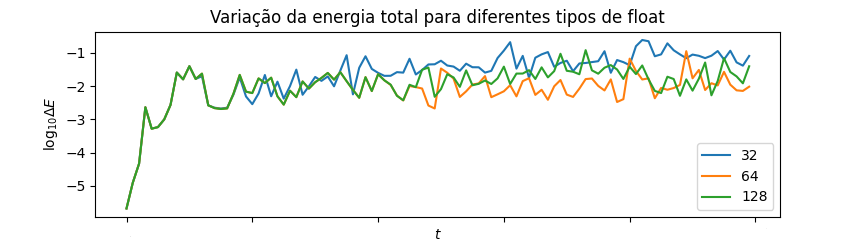
\includegraphics[width=\linewidth]{tcc//img/bits_energia.png}
    \caption{Variação da energia total no problema-modelo \ref{probmodelo:iau25} via método Ruth4 com $h=10^{-2}$ e $\epsilon=5h$ no intervalo $[0,500]$ para \textit{floats} com 32, 64 e 128 bits.}
    \label{fig:bits_energia}
\end{figure}

%%%%%%%%%%%%%%%%%%%%%%%%%%%%%%%%%%%%%
%%% PARALELIZAÇÃO
%%%%%%%%%%%%%%%%%%%%%%%%%%%%%%%%%%%%%
\subsection{Paralelização}\label{subsecao:paralelizacao}
Como mencionado anteriormente, foi utilizada uma biblioteca de Fortran para computação paralela, a \textit{OpenMP} (\textit{Open Multi-Processing}). Enquanto um código serial realiza uma operação por vez, um código paralelo é capaz de realizar mais de um cálculo ao mesmo tempo, como na figura \ref{fig:computacao_serial_paralela}. No caso do PCNG, existem algumas possibilidades para a aplicação: o cálculo do potencial e das forças, o cálculo da matriz normal utilizada no corretor numérico (ver equação (\ref{eq:corretor_matriz_normal})) e na detecção de colisões.

\begin{figure}[H]
    \centering
    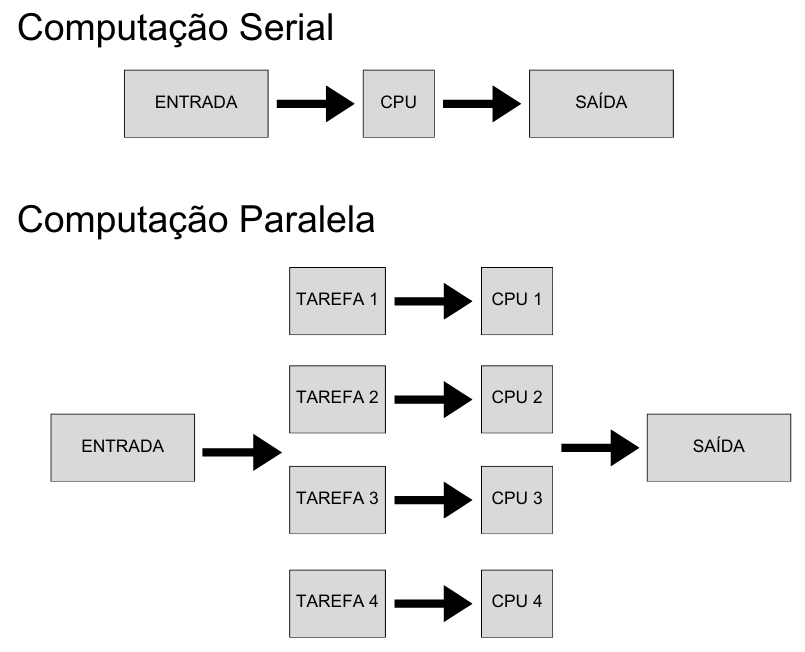
\includegraphics[width=0.5\linewidth]{tcc//img/computacao_serial_paralela.png}
        \caption{Visualização dos conceitos de computação serial e paralela.}
    \label{fig:computacao_serial_paralela}
\end{figure}

Exemplificando com o primeiro caso, foram implementadas duas funções de cálculo de forças: \verb|forcas_seq| e \verb|forcas_par|\footnote{O código completo consta em \cite{potalej_gravidade-fortran}.}. O núcleo do cálculo sequencial é feito da seguinte maneira:

\lstinputlisting[language=Fortran, caption=Código central da função sequencial de forças.]{tcc/codigos/forcas_seq.f90}

O valor \verb|distancia_inv| é o cubo do inverso da distância euclidiana entre os corpos, e \verb|Rab| é o vetor $\vet q_b - \vet q_a$. Observe como os \textit{loops} com \verb|DO| caracterizam a ordem quadrática dos cálculos. A proposta da paralelização neste caso está em dividir o cálculo da força para cada corpo entre os \textit{CPUs}, e posteriormente somar o resultado em um único vetor. Para isso, a biblioteca OpenMP permite definir variáveis compartilhadas (\verb|SHARED|, com as forças totais) e variáveis privadas (\verb|PRIVATE|, variáveis locais), o que garante que nenhuma CPU sobrescreva o vetor de forças das outras CPUs. A função paralelizada é semelhante à sequencial:

\lstinputlisting[language=Fortran, caption=Código central da função paralelizada de forças.]{tcc/codigos/forcas_par.f90}

Na figura \ref{fig:logtempo_paralelo_vs_sequencial} apresentamos um histograma em escala logarítmica com o tempo de computação (em segundos) para diferentes valores de $N$ com o método de Verlet e sem o uso de correção e de colisões, para garantir que o tempo esteja ligado diretamente com o cálculo das forças e do potencial. É possível observar que a diferença é expressiva para valores de $N$ a partir da centena, embora o cenário seja o oposto para valores de $N$ pequenos, uma vez que o custo de distribuir os cálculos entre os núcleos é maior que o do cálculo sequencial.

\begin{figure}
    \centering
    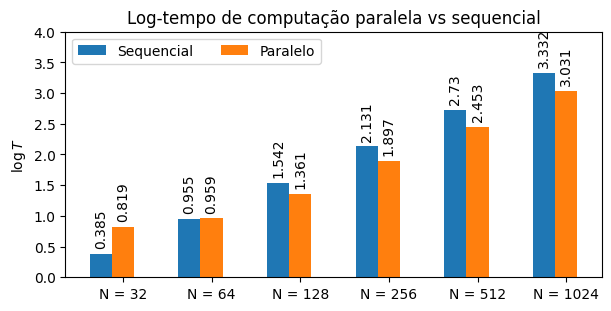
\includegraphics[width=0.8\linewidth]{tcc//img/logtempo.png}
    \caption{Log-tempo de computação paralela e computação sequencial para diferentes valores de $N$ e integração com método de Verlet, sem correção e sem colisão. Foram disponibilizados 4 núcleos para a paralelização.}
    \label{fig:logtempo_paralelo_vs_sequencial}
\end{figure}


%%%%%%%%%%%%%%%%%%%%%%%%%%%%%%%%%%%%%
%%% ARMAZENAMENTO
%%%%%%%%%%%%%%%%%%%%%%%%%%%%%%%%%%%%%
\subsection{Entrada e saída de dados}
Era objetivo que o programa final não contivesse somente simulações, mas facilitasse a geração de valores iniciais e a visualização dos dados também. Nesse sentido, há algumas opções disponíveis para a execução do programa, conforme tabela \ref{tabela:opcoes_entrada}.

\begin{table}
    \centering
    \begin{tabular}{c|c}
        \hline\hline
         \verb|-sv|, \verb|--sorteio-salvar|   & Sorteio de valores iniciais apenas \\
         \verb|-s|, \verb|--sorteio|           & Sorteio de valores iniciais e simulação \\
         \verb|-vi|, \verb|--valores-iniciais| & Simulação a partir de valores iniciais definidos \\
         \verb|-e|, \verb|--exibir|            & Exibição de trajetórias de uma simulação \\
         \verb|-d|, \verb|--dados|             & Exibição de dados de simulação \\
         \hline\hline
    \end{tabular}
    \caption{Opções de entrada no programa final.}
    \label{tabela:opcoes_entrada}
\end{table}

Existem também alguns tipos de arquivos diferentes utilizados pelo programa, os quais vale mencionar, conforme tabela \ref{tabela:arquivos_gerados}. Os arquivos do tipo 1 não são gerados, pois são o tipo mais simples, contendo informações como quantidade de corpos, valor das integrais primeiras, métodos \textit{etc}, sem definir valores iniciais explícitos.

\begin{table}
    \centering
    \begin{tabular}{c|c}
        \hline\hline
         1. & \textit{Preset} para sorteio \\
         2. & \textit{Preset} de valores iniciais \\
         3. & Informações de simulação (\textit{info.txt}) \\
         4. & Dados de simulação (\textit{data.csv}) \\
         \hline\hline
    \end{tabular}
    \caption{Arquivos utilizados ou gerados pelo programa.}
    \label{tabela:arquivos_gerados}
\end{table}

Os arquivos do tipo 1. podem ser usados para gerar valores iniciais explícitos através das chamadas \verb|-sv| e \verb|-s|, que têm entre as saídas um arquivo do tipo 2. Um exemplo de entrada consta no repositório do programa no diretório de \textit{presets}. Existem duas opções para a geração de valores iniciais: o sorteio \textit{comum} e o sorteio de \textit{Hénon}. No primeiro caso, apenas as integrais primeiras são condicionadas conforme o valor desejado. No segundo, são aplicadas as condições de Hénon, conforme descrito na seção \ref{secao:valores_iniciais}.

Já os arquivos de tipo 2 podem ser utilizados para as chamadas \verb|-vi|. Tais arquivos contêm configurações da simulação, como método, tamanho de passo e afins, e também os valores iniciais explícitos. O uso de tais arquivos facilita os testes com diferentes métodos para os mesmos valores iniciais.

Os arquivos de tipo 3 são gerados por simulações em ambas as chamadas \verb|-sv| e \verb|-vi|. Estes contêm informações acerca da simulação em si e de seu desempenho, podendo ser utilizados para comparações entre diferentes métodos. Por não ser um arquivo de entrada, é o que detém mais liberdade para conter diferentes informações. Um exemplo de arquivo de tipo 3 consta no programa \ref{prog:exemplo_saida}.

\lstinputlisting[label={prog:exemplo_saida}, caption={Exemplo de saída do arquivo de informações.}]{tcc/codigos/info.txt}

Por fim, os arquivos de tipo 4 contêm a constante $G$, o tamanho do passo, as massas, e as posições e momentos lineares no decorrer da simulação, armazenados no formato $(x, y, z, p_x, p_y, pz)$. Tais arquivos têm o formato \textit{.csv} (\textit{comma-separated values}). Esta não é a forma mais eficiente de armazenar dados do tipo, uma vez que a escrita de arquivos pelo Fortran é computacionalmente custosa e os arquivos ficam pesados. Para lidar com isso, existem tipos de arquivo mais eficientes, como o HDF\footnote{\textit{Hierarchical Data Format}. Para mais detalhes, veja: \href{https://www.hdfgroup.org/solutions/hdf5/}{https://www.hdfgroup.org/solutions/hdf5/}.}, mas por dificuldades técnicas e a facilidade de manipulação de CSV, a opção mais lenta foi escolhida.

%%%%%%%%%%%%%%%%%%%%%%%%%%%%%%%%%%%%%%%
%%% VALORES INICIAIS
%   Geracao de valores iniciais para o PNC. Condicionamento
%   de integrais primeiras, condições de Hénon, distribuições
%   para massas, posições e momentos.
%%%%%%%%%%%%%%%%%%%%%%%%%%%%%%%%%%%%%%%
%%%%%%%%%%%%%%%%%%%%%%%%%%%%%%%%%%%%%%%
%%% VALORES INICIAIS
%   Geracao de valores iniciais para o PNC. Condicionamento
%   de integrais primeiras, condições de Hénon, distribuições
%   para massas, posições e momentos.
%%%%%%%%%%%%%%%%%%%%%%%%%%%%%%%%%%%%%%%
\section{Valores iniciais}\label{secao:valores_iniciais}

O programa foi elaborado de modo que é possível entrar com valores iniciais de duas maneiras: diretamente e através de sorteios. Da primeira forma, é necessário informar cada massa, posição e momento linear inicial para cada corpo, o que é prático para problemas de poucos corpos mas inviável, a priori, conforme $N$ cresce, sendo necessário utilizar da segunda forma. Vale ressaltar que o sorteio também gera um arquivo de valores iniciais, então a primeira forma pode ser utilizada a posteriori.

Para gerar valores iniciais aleatórios é preciso escolher critérios que atendam as necessidades do problema que se objetiva simular. Para além de gerar valores utilizando, por exemplo, uma distribuição uniforme, muitas vezes é necessário também condicionar os valores gerados de modo que atendam determinada demanda, como os valores das integrais primeiras ou critérios iniciais para um sistema poder ser estável ou não. Tratamos esses dois casos a seguir.

%%%%%%%%%%%%%%%%%%%%%%%%%%%%%%%%%%%%%%%%%%%%%%%%%%%%
\subsection{Condicionamento das integrais primeiras}
Considere valores iniciais $(\vet m, \vet q, \vet p) \in \R_+^N \times \R^{3N} \times \R^{3N}$ obtidos através de um gerador com uma distribuição de probabilidade qualquer, que tenha integrais primeiras $E$, $\vet J$, $\vet P$ e $\vet G$, sendo $\vet G(t) = M \vet q_{cm} (t) - t \vet P$.

Começando por $\vet G$, é importante lembrar que o PNCG tem equações de movimento autônomas, então no instante inicial tem-se $\vet G = M \vet q_{cm}$. Assim, para obter $\tilde{\vet G}$ desejado basta que
\begin{equation*}
    \vet q_{cm}(0) = \dfrac{1}{M} \tilde{\vet G},
\end{equation*}
e para obter tal centro de massas basta transladar as coordenadas $\vet q_a$ individualmente:
\begin{equation*}
    \tilde{\vet q_a} = \vet q_a - \dfrac{1}{M} \left(\vet q_{cm}(0) - \tilde{\vet G}\right).
\end{equation*}

Como já dito anteriormente, o PNCG também é invariante por translações, uma vez que o potencial $V$ o é. Isso significa que utilizar como condição inicial $\vet q$ ou $\tilde{\vet q}$ não afeta a forma como o sistema evoluirá. Assim, uma facilidade bastante conveniente, como já feito anteriormente, é começar com o centro de massas na origem:
\begin{equation}\label{eq:condicionamento_rcm}
    \tilde{\vet q_a} = \vet q_a - \dfrac{1}{M} \vet q_{cm}(0)
    \Rightarrow
    \tilde{\vet G} = \vet 0.
\end{equation}

No caso de $\vet P$, para gerar um $\tilde{\vet P}$ é necessário obter $\tilde{\vet p}$ tal que $\tilde{\vet P} = \sum_{a=1}^{N} \tilde{\vet p_a}$. Então:
\begin{equation*}
    \tilde{\vet P} 
    = \vet P - \vet P + \tilde{\vet P}
    = \sum_{a=1}^{N} \vet p_a - \dfrac{c_a}{C}\left(\vet P - \tilde{\vet P}\right),
    \quad
    C = \sum_{a=1}^{N} c_a,
    \quad
    c_a > 0, \forall a.
\end{equation*}
As constantes $c_a$ podem ser quaisquer, correspondendo a pesos atribuídos a cada momento linear. No caso do PNCG, uma escolha conveniente de pesos é a massa de cada corpo, sendo então
\begin{equation}\label{eq:condicionamento_p}
    \tilde{\vet p_a} = \vet p_a - \dfrac{m_a}{M} (\vet P - \tilde{\vet P}).
\end{equation}

Para o momento angular total $\vet J$, embora para problemas planares baste aplicar 
\begin{equation*}
    \tilde{\vet p_a} = \vet p_a - \dfrac{m_a}{I} \vet q_a \times (\vet J - \tilde{\vet J})
\end{equation*}
para obter $\tilde{\vet J}$, no caso geral em três dimensões a situação é mais complicada. 

\begin{figure}
    \centering
    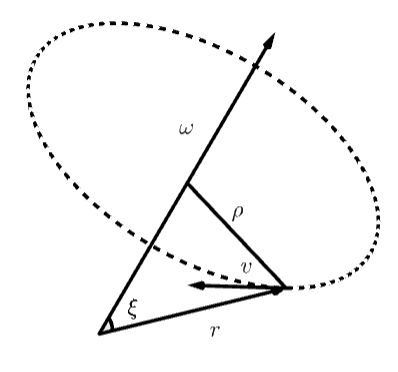
\includegraphics[width=0.3\linewidth]{tcc//img/rotacao.png}
    \caption{Situação descrita.}
    \label{fig:angular_rotacao}
\end{figure}

Considere uma partícula com posição $\vet r$ e um vetor $\vet \omega$ que define um eixo de rotação, do qual $\vet r$ se distancia em $\vet \rho$ e forma um ângulo $\xi$ e cuja velocidade da partícula a relação a é $\vet v$, como na figura \ref{fig:angular_rotacao}. Nessa situação, temos que $\norma{\vet v} = \rho \norma{\vet \omega}$ e $\sin \xi = \rho / \norma{\vet r}$. Uma vez que $\vet v \perp \vet \omega$ e $\vet v \perp \vet r$, podemos concluir que $\vet v \parallel \vet r \times \vet \omega$. Mais ainda, temos que:
\begin{equation*}
    \norma{\vet r \times \vet \omega} 
    = \norma{\vet r} \norma{\vet \omega} \sin \xi
    = \rho \norma{\vet \omega} = \norma{\vet v},
\end{equation*}
então
\begin{equation}\label{eq:velocidade_angular}
    \vet v = \vet r \times \vet \omega.
\end{equation}

O momento angular $\vet J$ também é um vetor perpendicular a $\vet r$ e a $\vet v$, mas $\vet J$ e $\vet \omega$ só são colineares quando $\vet r \perp \vet \omega$. Porém, a partir de (\ref{eq:velocidade_angular}), tem-se que $\vet J = m \vet r \times (\vet r \times \omega)$, então é possível construir um operador $\vet I: \R^3 \to \R^3$ a partir de $m$ e $\vet r$ que leva $\vet \omega$ em $\vet J$ como segue. Veja que
\begin{equation*}
    \vet r \times \vet \omega = (r_2 \omega_3 - r_3 \omega_2) \hat e_1 + (r_3 \omega_1 - r_1 \omega_3) \hat e_2 + (r_1 \omega_2 - r_2 \omega_1) \hat e_3,
\end{equation*}
então
\begin{align*}
    \vet J = m \vet r \times (\vet r \times \vet \omega) &=
    m \begin{bmatrix}
        r_2 r_1 \omega_2 - r_2^2 \omega_1 - r_3^2 \omega_1 + r_1 r_3 \omega_3 \\
        r_3 r_2 \omega_3 - r_3^2 \omega_2 - r_1^2 \omega_2 + r_1 r_2 \omega_1 \\
        r_1 r_3 \omega_1 - r_1^2 \omega_3 - r_2^2 \omega_3 + r_2 r_3 \omega_2
    \end{bmatrix} \\ &=
    m \begin{bmatrix}
        -(r_2^2 + r_3^2) & r_1 r_2 & r_1 r_3 \\
        r_1 r_2 & -(r_1^2 + r_3^2) & r_2 r_3 \\
        r_1 r_3 & r_2 r_3 & - (r_1^2 + r_2^2)
    \end{bmatrix}
    \begin{bmatrix}
        \omega_1 \\ \omega_2 \\ \omega_3
    \end{bmatrix}
    := \vet I \vet \omega.
\end{align*}

Tal aplicação $\vet I$ já é bem conhecida na literatura pelo nome de \textit{tensor de inércia}, fornecendo uma nova expressão para o momento angular. No caso de diversos corpos, a ideia é definir um eixo de rotação comum e a partir dele aplicar transformações sobre a velocidade angular de cada corpo. A primeira parte é simples, pois
\begin{equation*}
    \vet J = \sum_{a=1}^{N} \vet J_a = \sum_{a=1}^{N} \vet I_a \vet \omega = \vet I_{total} \vet \omega.
\end{equation*}

A partir disso, para obter um momento angular desejado $\tilde{\vet J}$ basta encontrar um eixo $\vet \omega$ tal que
\begin{equation*}
    \vet I_{total} \vet \omega = \vet J - \tilde{\vet J}
\end{equation*}
e aplicar a transformação
\begin{equation}\label{eq:condicionamento_j}
    \tilde{\vet p_a} = \vet p_a - m_a \vet q_a \times \vet \omega.
\end{equation}

A essa altura, é natural suspeitar que aplicar (\ref{eq:condicionamento_j}) depois de (\ref{eq:condicionamento_p}) mudaria o valor de $\tilde{\vet P}$ e vice-versa. Porém, considere o misto das aplicações:
\begin{equation}\label{eq:condicionamento_j_p}
    \tilde{\vet p_a} = \vet p_a - \dfrac{m_a}{M}(\vet P - \tilde{\vet P}) - m_a \vet q_a \times \omega.
\end{equation}

Temos:
\begin{align*}
    \sum_{a=1}^{N} \tilde{\vet p_a}
    & = \tilde{\vet P} - \vet q_{cm} \times \omega = \tilde{\vet P}
    \\
    \sum_{a=1}^{N} \vet q_a \times \tilde{\vet p_a}
    & = \tilde{\vet J} - \dfrac{1}{M} \vet q_{cm} \times (\vet P - \tilde{\vet P}) = \tilde{\vet J},
\end{align*}
pois $\vet q_{cm} = \vet 0$. Assim, com o centro de massas na origem, é possível condicionar o momento linear total e o momento angular total separadamente.

Já para a energia total $E$, existem dois caminhos possíveis: aplicar transformações sobre as posições ou sobre os momentos lineares. Uma vez que $E$ é separável, isto é,
\begin{equation*}
    E(\vet q, \vet p) = T(\vet p) + V(\vet q),
\end{equation*}
e que as funções $T$ e $V$ têm sinais opostos no PNCG, existem muitas formas diferentes de balancear a energia total. Para obter uma energia total negativa, por exemplo, basta aproximar os corpos, mas pode ser suficiente reduzir as velocidades em vez disso. Já para uma energia total positiva, basta aumentar as velocidades, mas também pode ser possível apenas distanciar os corpos. No geral, tomando $\tilde{\vet q} = \alpha^{-1} \vet q$ e $\tilde{\vet p} = \beta \vet p$, tem-se:
\begin{equation*}
    \tilde E := E(\tilde{\vet q}, \tilde{\vet p}) = \beta^2 T(\vet p) + \alpha V (\vet q) = \beta^2 (E_0 - V_0) + \alpha V_0.
\end{equation*}

Neste trabalho, a solução aplicada para esse dilema foi aplicar a transformação necessária para as velocidades, e se a energia desejada for diferente de zero então é aplicada uma aproximação ou distanciamento entre os corpos. Na prática, isso foi dado pelo seguinte:
\begin{equation*}
    \beta = \sqrt{\dfrac{-V_0}{T(\vet p_0)}},
    \quad
    \alpha = 1 + \dfrac{\tilde E}{V_0}
\end{equation*}
Um questionamento cabível é o quanto essa escolha afetou os resultados obtidos, uma vez que existem diversas outras transformações possíveis. Não chegamos a testar outros valores, então no momento não temos resposta para isso. 

A transformação que condiciona a energia total afeta os momentos linear e angular totais:
\begin{equation*}
    \sum_{a=1}^{N} \tilde{\vet p_a} = \beta \vet P,
    \quad
    \sum_{a=1}^{N} \tilde{\vet q_a} \times \tilde{\vet p_a} = \dfrac{\beta}{\alpha} \vet J.
\end{equation*}

Este problema é de fácil resolução, pois basta que $\tilde{\vet P}$ e $\tilde{\vet J}$ sejam multiplicados pelas devidas constantes na equação (\ref{eq:condicionamento_j_p}), gerando a seguinte mudança de coordenadas:
\begin{align}
    \tilde{\vet q_a} &= \dfrac{1}{\alpha}\left(\vet q_a - \dfrac{1}{M} \vet q_{cm} (0)\right), \\
    \tilde{\vet p_a} &= \beta\left( \vet p_a - \dfrac{m_a}{M} \left(\vet P - \dfrac{\tilde P}{\beta}\right) - m_a \vet q_a \times \vet \omega \right), \\
    \vet I_{total} \vet \omega &= \vet J - \dfrac{\tilde{\vet J} \alpha}{\beta}, \\
    \alpha = 1 + \dfrac{\tilde E}{V_0}, 
    & \quad
    \label{eq:beta_1} \beta = \sqrt{\dfrac{- V_0}{T( \tilde{\vet p_a} / \beta)}}
\end{align}

Observe que $\beta$ fica definido implicitamente pela equação (\ref{eq:beta_1}). Elevando os dois lados ao quadrado é possível isolar $\beta$, obtendo-se a seguinte expressão:
\begin{equation}
    \beta = \pm \sqrt{- \dfrac{V_0 + S_2}{S_1}},
\end{equation}
onde
\begin{align*}
    S_1 &= \sum_{a=1}^{N} \dfrac{1}{2 m_a} \norma{\vet K_1^a}^2 
    = \sum_{a=1}^{N} \dfrac{1}{2 m_a} \norma{\vet p_a - \dfrac{m_a}{M} \vet P - m_a q_a \times (\bm I_{total}^{-1} \vet J)}^2, 
    \\
    S_2 &= \sum_{a=1}^{N} \dfrac{1}{2 m_a} \norma{\vet K_2^a}^2
    = \sum_{a=1}^{N} \dfrac{1}{2 m_a} \norma{\dfrac{m_a}{M} \tilde{\vet P} + \alpha m_a \vet q_a \times (\bm I_{total}^{-1} \tilde{\vet J})}^2,
    \\
    \sum_{a=1}^{N} & \dfrac{1}{m_a} \prodint{\vet K_1^a}{\vet K_2^a} = 0.
\end{align*}

A escolha do sinal de $\beta$ define a evolução do sistema, uma vez que a velocidade de cada partícula é multiplicada por $\beta$. O sistema com $\beta < 0$ é o equivalente de simular o caso $\beta > 0$ utilizando um tamanho de passo $h^- < 0$ para integradores reversíveis, ou seja, escolhido um sinal de $\beta$, o seu oposto equivale a integrar o sistema no sentido temporal oposto. Em termos de posições, porém, conseguimos uma única configuração que atende às expectativas de integrais primeiras e tem centro de massas centrado na origem. Veja um exemplo do mencionado na figura \ref{fig:vi-betas}.

\begin{figure}
    \centering
    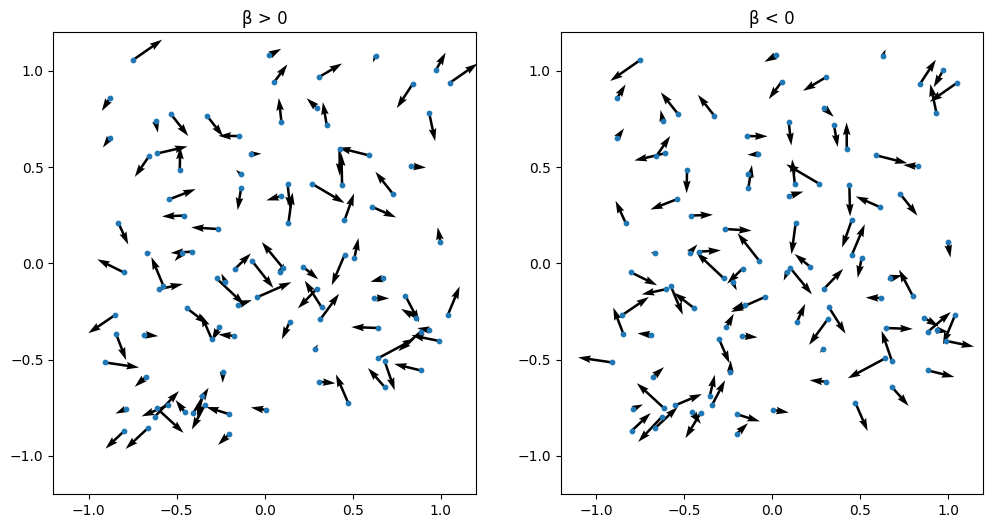
\includegraphics[width=0.8\linewidth]{tcc//img/100corpos_betas.png}
    \caption{Posições e momentos lineares em um problema de 100 corpos com todas as integrais primeiras nulas para os dois valores de $\beta$.}
    \label{fig:vi-betas}
\end{figure}




%%%%%%%%%%%%%%%%%%%%%%%%%%%%%%%%%%%%%%
\subsection{Condições de estabilidade}\label{subsection:condicoes_aarseth}
Em busca de um sistema de unidades padrão que permitisse a comparação de resultados obtidos por diferentes pesquisadores do PNCG, \citep{Hnon1972, Heggie} propõem utilizar o seguinte:
\begin{equation*}
    G = 1, \quad
    M = 1, \quad
    R_V = 1.
\end{equation*}
sendo $R_V$ o raio de virial. Isso significa que temos o seguinte, conforme equação (\ref{eq:raio_virial}):
\begin{equation*}
    V \approx - \dfrac{G M^2}{2 R_V} = - \dfrac{1}{2},
\end{equation*}
e pelo Teorema do Virial (Teorema \ref{teorema:virial}) para uma relação de equilíbrio instantânea:
\begin{equation*}
    T = - \dfrac{1}{2} V \approx \dfrac{1}{4} 
    \Rightarrow
    E = - \dfrac{1}{4}.
\end{equation*}

Para sistemas com essas condições iniciais, é esperado que, com alguma regularização em uso (como o amortecimento do potencial, por exemplo), o sistema fique limitado - ou seja, \textit{estável} -, ao menos temporariamente.

Os testes apresentados nas próximas subseções nos quais as massas são iguais e somam 1 utilizam as condições de Hénon.


%%%%%%%%%%%%%%%%%%%%%%%%%%%%%%%%%%%%%%%
%%% COLISOES
%   Aplicacao das colisoes e criterios. Exemplos do uso
%   para problemas de poucos corpos e problemas de varios
%   corpos. Custo computacional e eficiencia.
%%%%%%%%%%%%%%%%%%%%%%%%%%%%%%%%%%%%%%%
%%%%%%%%%%%%%%%%%%%%%%%%%%%%%%%%%%%%%%%
%%% COLISOES
%   Aplicacao das colisoes e criterios. Exemplos do uso
%   para problemas de poucos corpos e problemas de varios
%   corpos. Custo computacional e eficiencia.
%%%%%%%%%%%%%%%%%%%%%%%%%%%%%%%%%%%%%%%
\section{Colisões}\label{section:simulacao_colisoes}
Como inicialmente discutido na seção \ref{section:pncg_colisoes}, existem algumas formas de lidar com colisões no PNCG e que se aplicam para aproximações muito intensas, ou \textit{quase colisões}, uma vez que o conjunto de valores iniciais que levam a uma colisão em tempo finito têm medida zero. A abordagem com colisões elásticas é uma delas.

Para utilizar colisões, como já dito, um meio natural é definir uma densidade $\rho$ para a massa de modo que
\begin{equation}
    r_a = \sqrt[3]{\dfrac{3 m_a}{4 \pi \rho}}
\end{equation}
é o raio de um corpo esférico de massa $m_a$. Cada escolha de densidade possível gera um conjunto de trajetórias diferentes, uma vez que uma aproximação intensa que é considerada como colisão para um certo $\rho_1$ pode não o ser para um $\rho_2$ diferente. Porém, este método possui a vantagem de garantir a reprodutibilidade das simulações.

Um problema de utilizar colisões elásticas é que nem sempre o raio é o suficiente para detectar uma colisão ou quase-colisão antes que o estrago numérico seja feito. Pode acontecer, por exemplo, de em um instante $t$ dois corpos estarem distantes o suficiente para não haver colisão mas no instante $t + \delta t$ os dois volumes associados aos corpos terem uma interseção não vazia no espaço de configurações - na prática, um corpo \textit{entrar} no outro, como na figura \ref{fig:colisao_intersecao}. Uma tática que pode ser utilizada para evitar isso é: uma vez detectada a interseção, interpolar as trajetórias entre os instantes $t$ e $t+\delta t$, obtendo assim o exato momento da colisão $t \leq t^* \leq t+\delta t$, aplicar a colisão em $t^*$ e substituir a trajetória com interseção em $t + \delta t$ pela trajetória em que houve colisão no instante $t^*$. Embora não exista dificuldade teórica em tal tática, aplicá-la numericamente é um desafio, especialmente em problemas de muitos corpos, pois todo esse processo é, além de custoso, computacionalmente complicado de ser avaliado, por isso não foi utilizado.

\begin{figure}
    \centering
    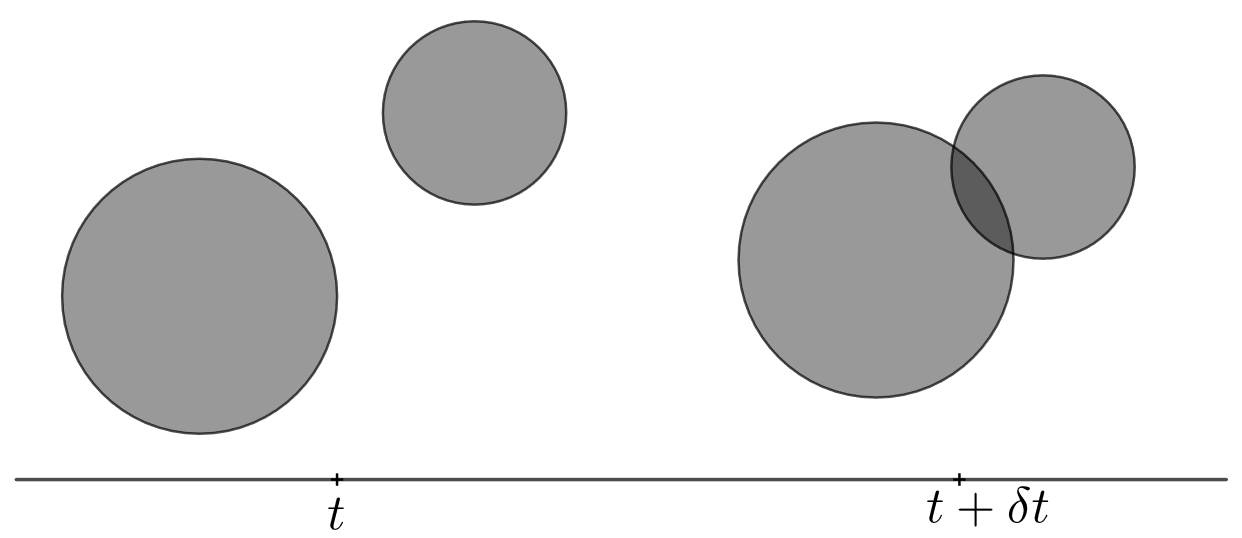
\includegraphics[width=0.7\linewidth]{tcc//img/colisao_intersecao.png}
    \caption{Problema descrito, onde o instante de colisão exato $t^*$ é tal que $t \leq t^* \leq t + \delta t$}
    \label{fig:colisao_intersecao}
\end{figure}

Outra saída mais simples para o problema é: uma vez detectada uma aproximação no instante $t+\delta t$ intensa o suficiente para desestabilizar numericamente o sistema antes de uma colisão elástica surtir efeito, voltar para o instante $t$ e aplicar a colisão elástica neste instante. Existem dois problemas com essa tática: é preciso escolher mais um valor $\epsilon_E$ (ligado à energia) para poder definir o que é uma \textit{desestabilização} considerável e é possível que retornar ao passo anterior resolva o problema de imediato, mas jogue a partícula colidida em rota de colisão com outra partícula, gerando uma situação recursiva.

O primeiro problema poderia ser resolvido com estatística, identificando uma ``desestabilização'' como um \textit{outlier} numa estatística suficiente para a energia, por exemplo, ou com o rigor dos integradores numéricos, pois cada integrador tem um teto para o erro das trajetórias e consequentemente um teto para o erro da energia total, sendo uma ``desestabilização'' qualquer coisa acima dessa margem. A solução estatística chegou a ser brevemente testada mas não ofereceu resultados satisfatórios, uma vez que trouxe mais um custo computacional e não foi capaz de se livrar do segundo problema. A solução com teto dos integradores não foi implementada por dificuldades teóricas em determinar o teto, mas pretendemos avaliar essa medida de erro de cada método no futuro.

Uma última questão com as colisões elásticas é o custo de identificar seu acontecimento. Da mesma forma que o potencial e as forças, são necessárias $N (N-1) / 2$ verificações para identificar uma colisão, sendo então mais uma operação computacionalmente custosa. Existem outras formas mais eficientes de detectar colisões e há toda uma literatura voltada para isso, como \cite{Ericson2005}, pois existe uma gama de aplicações que necessitam de métodos eficientes para detecção de colisões. Para este trabalho, por facilidade, foi utilizada a verificação um-a-um comentada.

Existem outras regularizações que permitem lidar com colisões, especialmente colisões binárias, como a transformação de Levi-Civita (para problemas planares), sua generalização no método de Kustaanheimo-Stiefel e a alternativa pelo método de Burdet-Heggie \citep{aarseth_gravitational_2003}. Nenhuma dessas regularizações foi estudada a fundo então estas não serão tratadas neste trabalho. Para mais detalhes, a referência de Aarseth é recomendada para os três métodos mencionados, tendo o seu capítulo 4 totalmente voltado para este problema.

Há também outra forma de evitar colisões e quase-colisões, que é impondo um limite sobre o potencial. Tomando $\epsilon > 0$, definimos o potencial amortecido
\begin{equation}
    V_\epsilon = - G \sum_{a < b} \dfrac{m_a m_b}{\sqrt{r_{ab}^2 + \epsilon^2}},
\end{equation}
o que gera as forças
\begin{equation}
    \derpar{V}{\vet q_a} = G \sum_{b \neq a} m_a m_b \dfrac{\vet q_b - \vet q_a}{(r_{ab}^2 + \epsilon^2)^{3/2}}.
\end{equation}

Observe que apesar da diferença nos cálculos, a energia total amortecida $E_\epsilon = T + V_\epsilon$ ainda é conservada, pois
\begin{equation*}
    \der{E_\epsilon}{t} 
    = \nabla_{\vet p} T \cdot \dvet p + \nabla_{\vet q} V_\epsilon \cdot \dvet q
    = 0.
\end{equation*}

O uso de um amortecimento pode levantar dúvidas naturais a respeito da precisão dos resultados obtidos com simulações. É fato que o mesmo conjunto de valores iniciais leva a um resultado quando usado o potencial $V$ e a outro resultado quando usado o potencial $V_\epsilon$. Porém, quando o interesse está nas propriedades dinâmicas do sistema e não em trajetórias individuais - o que no geral ocorre para valores de $N$ suficientemente grandes -, $\epsilon$ precisa ser relativamente grande para que o resultado final seja notavelmente diferente \citep[235]{aarseth_gravitational_2003}.

Dessa forma, tanto a colisão elástica quanto o potencial amortecido conservam a energia de alguma forma, então foram implementados no programa final. Cabe observar que uma possível solução para se livrar de alguns dos problemas comentados no uso de colisões elásticas é utilizar um método híbrido que incorpore o amortecimento, além de utilizar o corretor para amenizar a instabilidade do potencial. Ainda assim, é esperado que as órbitas individuais sejam diferentes, mesmo que as integrais primeiras sejam as mesmas. Um exemplo pode ser visto na figura \ref{fig:iau25_trajetorias_colisoes}.

\begin{figure}
    \centering
    \begin{subfigure}{.5\textwidth}
      \centering
      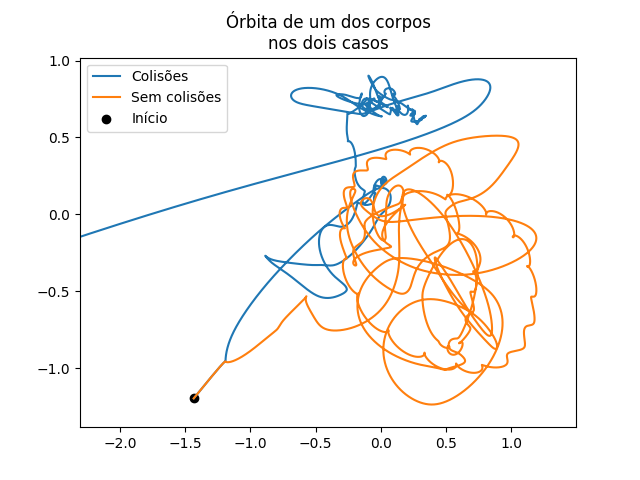
\includegraphics[width=\linewidth]{tcc/img/trajetoria_iau25_colisao_vs_sem_colisao.png}
      % \caption{Órbita de um dos corpos nos dois casos.}
      \caption{}
      \label{fig:iau25_trajetorias_colisoes_a}
    \end{subfigure}%
    \begin{subfigure}{.5\textwidth}
      \centering
      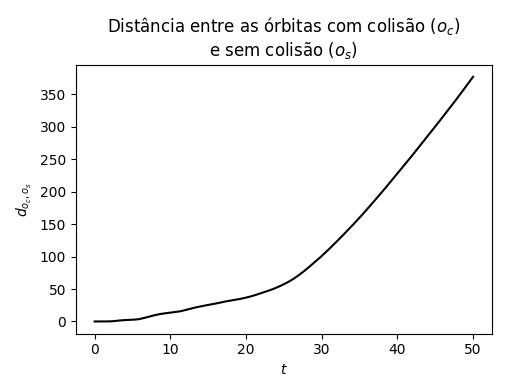
\includegraphics[width=\linewidth]{tcc/img/distancia_orbitas_iau25.png}
      % \caption{Distância entre as órbitas no espaço de fases.}
      \caption{}
      \label{fig:iau25_trajetorias_colisoes_b}
    \end{subfigure}
    
    \caption{Simulações do problema-modelo \ref{probmodelo:iau25} via método RKN671 com $h=10^{-3}$, $\epsilon=5h$ e corretor com margem de erro da energia $10^{-10}$ no intervalo $[0,50]$. Em um dos casos utilizou-se colisões ativadas com $r_a = 5h$, $a=1,2,...,N$ e no outro as colisões estavam desativadas.}
    \label{fig:iau25_trajetorias_colisoes}
\end{figure}

%%%%%%%%%%%%%%%%%%%%%%%%%%%%%%%%%%%%%%%
%%% SOBRE O CORRETOR NUMÉRICO
%   Questões práticas do corretor
%%%%%%%%%%%%%%%%%%%%%%%%%%%%%%%%%%%%%%%
%%%%%%%%%%%%%%%%%%%%%%%%%%%%%%%%%%%%%%%
%%% Corretor numérico
%   Questões práticas sobre o uso do
%   corretor numérico.
%%%%%%%%%%%%%%%%%%%%%%%%%%%%%%%%%%%%%%%
\section{Uso do corretor numérico}\label{secao:uso_do_corretor}
O corretor numérico apresentado na seção \ref{secao:corretor_numerico} possui algumas questões sobre sua usabilidade no programa que valem ser discutidas nesta seção. Para começar, é interessante que o uso de um corretor numérico não eleve drasticamente o tempo necessário para realizar uma simulação. No caso deste corretor, existem alguns custos associados.

O primeiro é no cálculo das integrais primeiras. Embora $\vet \Psi(\vet z_0)$ seja calculado apenas uma vez, a cada iteração que utiliza o corretor é necessário calcular $\vet \Psi(\vet z)$. O cálculo direto da energia total para um potencial de N-corpos, por exemplo, tem ordem $O(N^2)$ de operações, podendo ser então um custo relevante.

Um segundo custo é na resolução do sistema linear (\ref{eq:corretor_equacao_2}), pois a matriz jacobiana $D \vet \Psi$ tem tamanho $k \times 6N$. Observe, porém, que a matriz
\begin{equation}\label{eq:corretor_matriz_normal}
    \vet \Gamma (\vet z) = D \vet \Psi(\vet z) D \vet \Psi(\vet z)^T
\end{equation}
é uma matriz normal, e seu tamanho é $k \times k$. Além disso, cada elemento seu é dado diretamente por um produto interno:
\begin{equation*}
    \vet \Gamma_{ij} = \prodint{\nabla \psi_i}{\nabla \psi_j},
\end{equation*}
o que a caracteriza como uma matriz de Gram, e também em casos com poucas integrais primeiras de interesse isso significa que esta pode ser calculada manualmente, otimizando uma parte do processo. 

Além disso, a resolução do sistema de equações
\begin{equation*}
    \bm \Gamma (\vet y) \vet \alpha = \vet \Psi(\vet z) - \vet \Psi(\vet z_0).
\end{equation*}
também possui um custo associado, o que depende da quantidade de integrais primeiras utilizadas e do método utilizado para resolução. A primeira abordagem computacional tomada foi utilizar a sub-rotina \verb|dgesv|, do LAPACK, a qual resolve um sistema $\bm A \vet x = \vet b$, com $\bm A$ $n \times n$ aplicando a decomposição LU sobre $\bm A$, o que tem custo $O(n^3)$, e resolvendo o sistema triangular restante, com custo $O(n^2)$.

Porém, uma vez que a matriz $\bm \Gamma$ é de Gram, é também no mínimo positiva semi-definida. Isso significa que em vez de utilizar LU, que tem como fundo o pivoteamento gaussiano, faz sentido utilizar a decomposição de Cholesky, que apesar de ter $O(n^3)$ consome apenas metade das operações do pivoteamento gaussiano, e trata-se de um algoritmo que sempre é numericamente estável \citep[172-177]{Trefethen1997}. No LAPACK, as subrotinas utilizadas para isso foram \verb|dpotrf| (para a fatoração de Cholesky) e \verb|dpotrs| (para a resolução de um sistema linear Cholesky-fatorado). 

Realizamos alguns testes com os dois métodos de resolução mas não encontramos diferenças expressivas. Um exemplo de aplicação foi em um problema de $10^3$ corpos com condições de Hénon (ver seção \ref{secao:valores_iniciais}), e o resultado pode ser encontrado na figura \ref{fig:corretor_cholesky_vs_lu_energia} e na tabela \ref{tab:corretor_cholesky_vs_lu_energia}. Vale ressaltar que, quanto ao desempenho, ambas as simulações levaram por volta de 10,4 minutos, com uma pequena vantagem de alguns segundos para o uso de Cholesky.

\begin{figure}
    \centering
    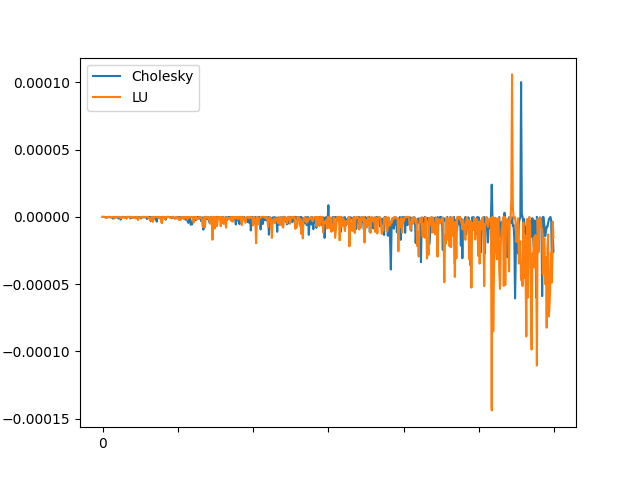
\includegraphics[width=0.5\linewidth]{tcc//img/exemplo_cholesky_vs_lu_energia.png}
    \caption{Variação da energia $\Delta E$ em um problema de $10^3$ corpos utilizando o integrador Velocity-Verlet (2ª ordem), $h=0.1$ e $\epsilon=0.04$, com margem de erro da energia $10^{-11}$.}
    \label{fig:corretor_cholesky_vs_lu_energia}
\end{figure}

\begin{table}[]
    \centering
    \begin{tabular}{c|cc}
                      & Cholesky     & LU           \\ \hline
        Média         & $-3.639 \cdot 10^{-06}$ & $-6.656 \cdot 10^{-06}$ \\
        Mediana       & $-1.208 \cdot 10^{-06}$ & $-1.277 \cdot 10^{-06}$ \\
        Desvio padrão & $8.599 \cdot 10^{-06}$  & $1.551 \cdot 10^{-05}$  
    \end{tabular}
    \caption{Estatísticas sobre o valor $\Delta E$, nas condições da figura \ref{fig:corretor_cholesky_vs_lu_energia}.}
    \label{tab:corretor_cholesky_vs_lu_energia}
\end{table}

Diante do custo, vale questionar também se de fato faz sentido utilizar todas as integrais primeiras no corretor. Por mais que mais informações devam levar a uma correção melhor, uma integral primeira que seja numericamente estável pode ser só um custo a mais e não trazer resultados tão diferentes do que sem o seu uso. 

No PNCG, o centro de massas e o momento linear total são numericamente bem-comportados por serem lineares, e o momento angular também é estável por ser uma expressão livre de singularidades, como exemplificado na figura \ref{fig:var_integrais_es_iau25} da seção \ref{secao:integradores_simpleticos}. A energia total, por outro lado, é bastante instável em aproximações intensas devido ao potencial ser inversamente proporcional às distâncias. Dessa forma, como sugere \cite{Nacozy1972}, aplicar a correção somente na energia total no PNCG é, no geral, suficiente. O vetor de correção $\alpha$ (que é um escalar nesse caso) possui uma forma explícita:
\begin{equation}
    \alpha = \dfrac{E(\vet z) - E(\vet z_0)}{\norma{\nabla E(\vet z)}^2}.
\end{equation}
Um exemplo de aplicação no problema-modelo \ref{probmodelo:iau25} com as duas formas de correção pode ser visualizado na figura \ref{fig:var_energia_iau25_corretores}.

\begin{figure}
    \centering
    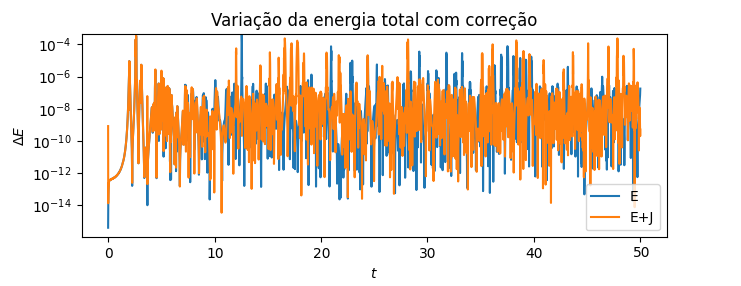
\includegraphics[width=\linewidth]{tcc/img/var_energia_todas_vs_energia_iau25.png}
    % \caption{RKN671 H=0.001, E=0.1, [0,50], COR=1E-10}
    \caption{Variação da energia no problema-modelo \ref{probmodelo:iau25} simulado via método RKN671 com $h=10^{-3}$, $\epsilon = 10^{-1}$ e com margem de erro da energia $10^{-10}$ no intervalo $[0,50]$. Em azul, foi aplicada a correção somente na energia total, enquanto em laranja foi aplicada a correção também no momento angular total.}
    \label{fig:var_energia_iau25_corretores}
\end{figure}

De toda forma, o custo do corretor só ocorre quando este é aplicado, então um bom critério de aplicabilidade pode reduzir o custo do corretor através da sua utilização somente quando estritamente necessário. No problema-modelo utilizado por Nacozy, o corretor era aplicado quando o erro da energia total atingia um valor por volta de 100 vezes menor que o erro de truncamento desejado. Constatamos empiricamente que com o uso do amortecimento no potencial, uma vez que o potencial deixa de ter singularidades, o teto pode ser tanto quanto desejado, então a escolha de Nacozy é razoável para o PNCG.

A implementação do corretor numérico é a sub-rotina \verb|correcao|, que depende de outras sub-rotinas de mecânica do programa.

%%%%%%%%%%%%%%%%%%%%%%%%%%%%%%%%%%%%%%%
%%% OUTROS ASPECTOS PRATICOS DO PNCG [NAO INCLUIDO]
%   Falar do tamanho de passo
%%%%%%%%%%%%%%%%%%%%%%%%%%%%%%%%%%%%%%%
% \section{Outros aspectos práticos do PNCG}

Além do tratado, existem questões práticas da simulação do PNCG que valem ser mencionadas, como a escolha do tamanho de passo. [ Escrever melhor]

A escolha de um tamanho de passo define

%%%%%%%%%%%%%%%%%%%%%%%%%%%%%%%%%%%%%%%
%%% SIMULACAO DA DINAMICA DE FORMAS
%   Falar sobre a simulacao da dinamica
%   de formas
%%%%%%%%%%%%%%%%%%%%%%%%%%%%%%%%%%%%%%%
\section{Aplicação: Dinâmica de Formas}\label{secao:simulacao_dinamica_de_formas}

Na seção \ref{secao:dinamica_de_formas} apresentamos uma breve introdução à Dinâmica de Formas sobre o PNCG, onde introduzimos a \textit{complexidade} $C_S$ como uma medida de evolução de um sistema e também as \textit{coordenadas objetivas} $(\vet \sigma, \vet \pi)$ sobre o espaço de formas. Nesta seção, visualizaremos alguns dos resultados apresentados.

Todas as simulações utilizadas aqui foram feitas com momento angular total $\vet J = \vet 0$, momento linear total $\vet P = \vet 0$ e centro de massas $\vet q_{cm} = \vet 0$. A energia foi testada com diferentes valores para diferentes objetivos, e os valores são explicitados em cada caso.



%%%%%%%% PROBLEMAS DE 3 CORPOS
\subsection{Problemas de 3 corpos}

Para visualizar as coordenadas objetivas $(\vet \sigma, \vet \pi)$, tomamos primeiramente um problema de 3 corpos com uma trajetória simples: um par kepleriano e um corpo ejetado, como na figura \ref{fig:probmodel_3_corpos_energia0_trajetoria}. Trata-se do problema-modelo \ref{probmodelo:3corpos_energia_nula}, integrado no intervalo $[0,50]$ via método de Verlet com $h=10^{-3}$, sem correção.

Este é um sistema com energia total 0, então os resultados da Dinâmica de Formas se aplicam. Por exemplo, a ejeção de um dos corpos corresponde a um atrito no espaço de fases (tomando a coordenada $\vet \omega$). Além disso, a complexidade (figura \ref{fig:3corpos_energia0_complexidade}) aumenta no sentido futuro devido à separação do sistema em dois, embora possua fortes oscilações ligadas às aproximações do sistema binário.

\begin{figure}[H]
    \centering
    
    \begin{subfigure}{.5\textwidth}
        \centering
        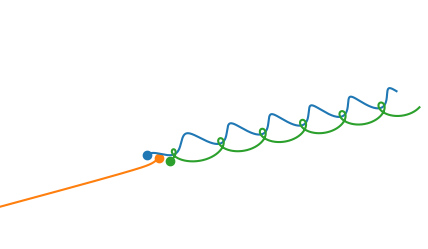
\includegraphics[width=0.8\linewidth]{tcc/img/sd/3corpos_energia0_posicoes_nd_2.png}
        \caption{}
        \label{fig:probmodel_3_corpos_energia0_trajetoria}
    \end{subfigure}%
    \begin{subfigure}{.5\textwidth}
        \centering
        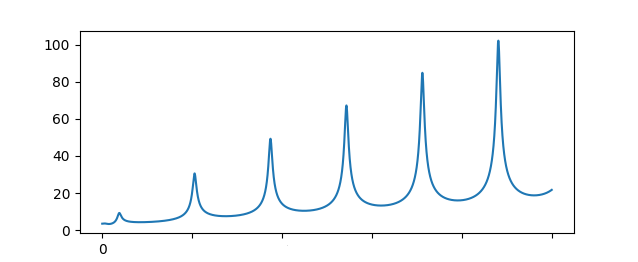
\includegraphics[width=\linewidth]{tcc/img/sd/3corpos_energia0_complexidade.png}
        \caption{}
        \label{fig:3corpos_energia0_complexidade}
    \end{subfigure}

    \caption{Problema-modelo \ref{probmodelo:3corpos_energia_nula}. À esquerda, recorte das trajetórias. À direita, a complexidade apresentada pelo sistema.}
    \label{fig:figuras_probmodel_3_energia0}
\end{figure}

Na figura \ref{fig:3corpos_energia0_posicoes_sd} é possível observar os comportamentos de ejeção e de formação de binários. Embora o corpo ejetado se afaste a princípio, conforme o par binário se forma, o ejetado desacelera e inicia uma trajetória cíclica e dissipativa. E, de fato, conforme a figura \ref{fig:3corpos_energia0_velocidades_sd} mostra, o corpo ejetado está desacelerando, enquanto o momento de forma ($\vet \pi$) dos outros dois apresenta trajetórias circulares com um raio cada vez maior e cada vez mais rapidamente. 

\begin{figure}[H]
    \centering
    \begin{subfigure}{.5\textwidth}
        \centering
        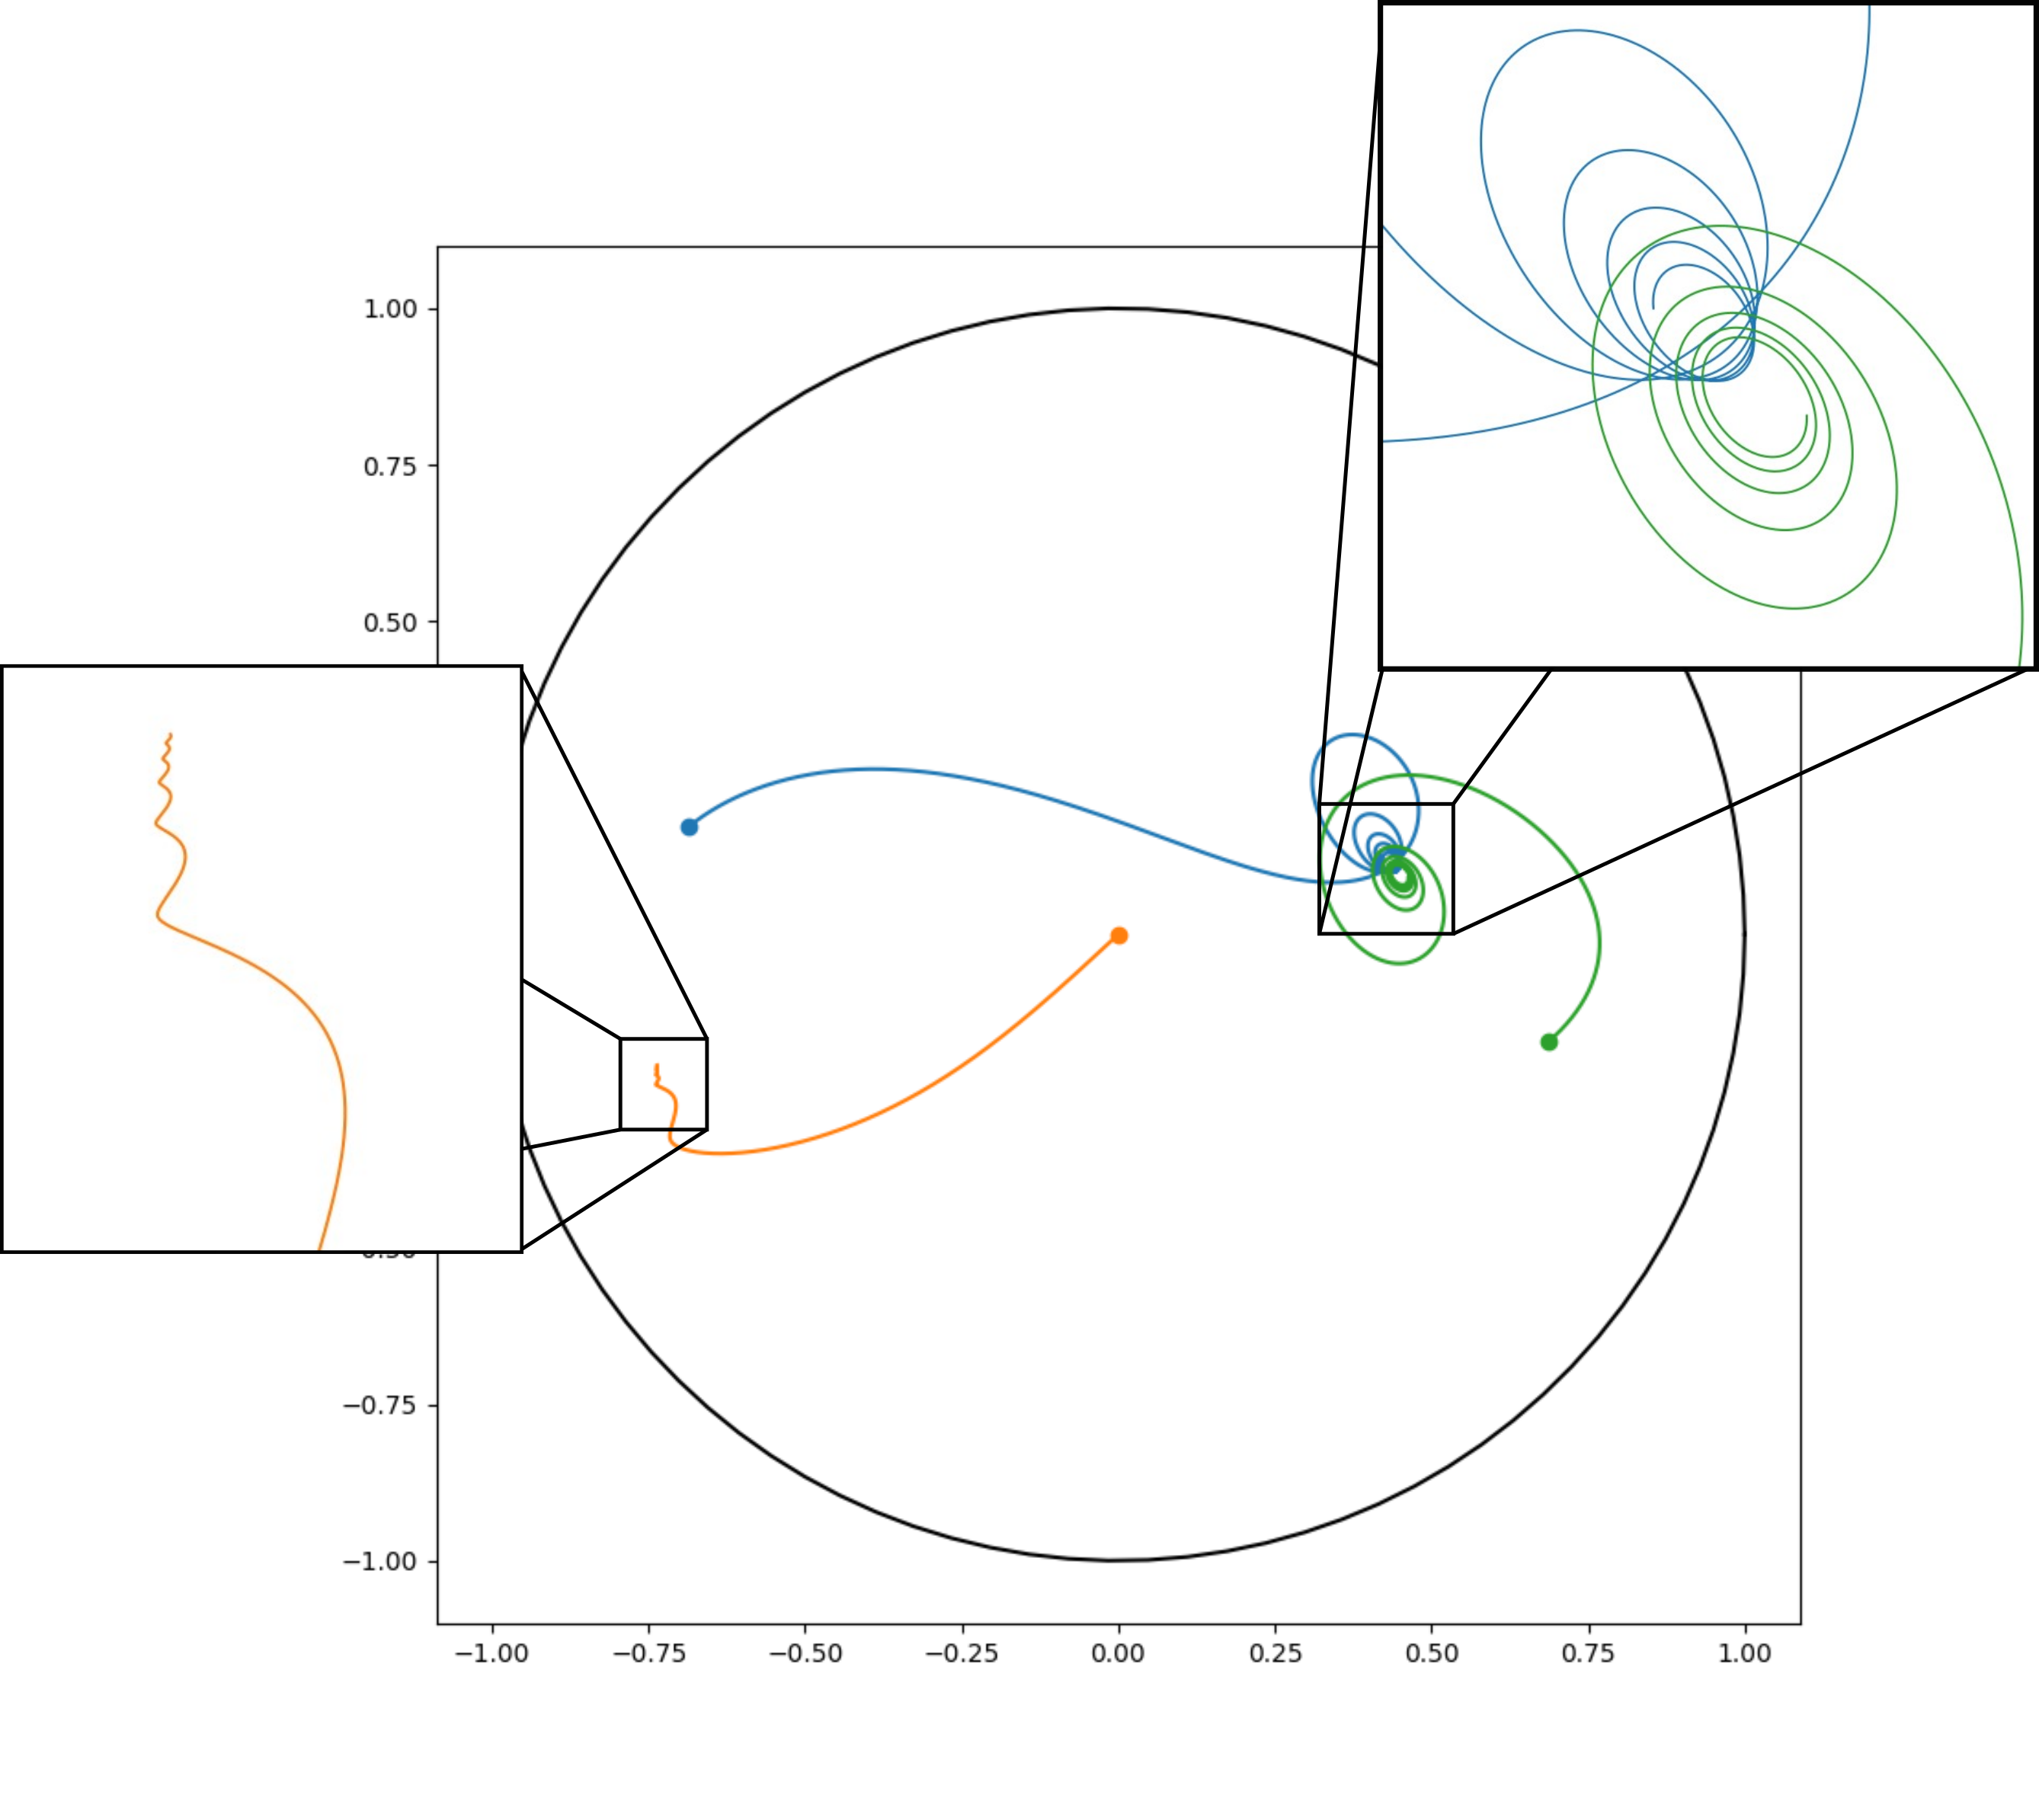
\includegraphics[width=\linewidth]{tcc//img/3corpos_energia0_posicoes_sd_zoom.png}
        \caption{Coordenadas de forma ($\vet \sigma$).}
        \label{fig:3corpos_energia0_posicoes_sd}
    \end{subfigure}%
    \begin{subfigure}{.5\textwidth}
        \centering
        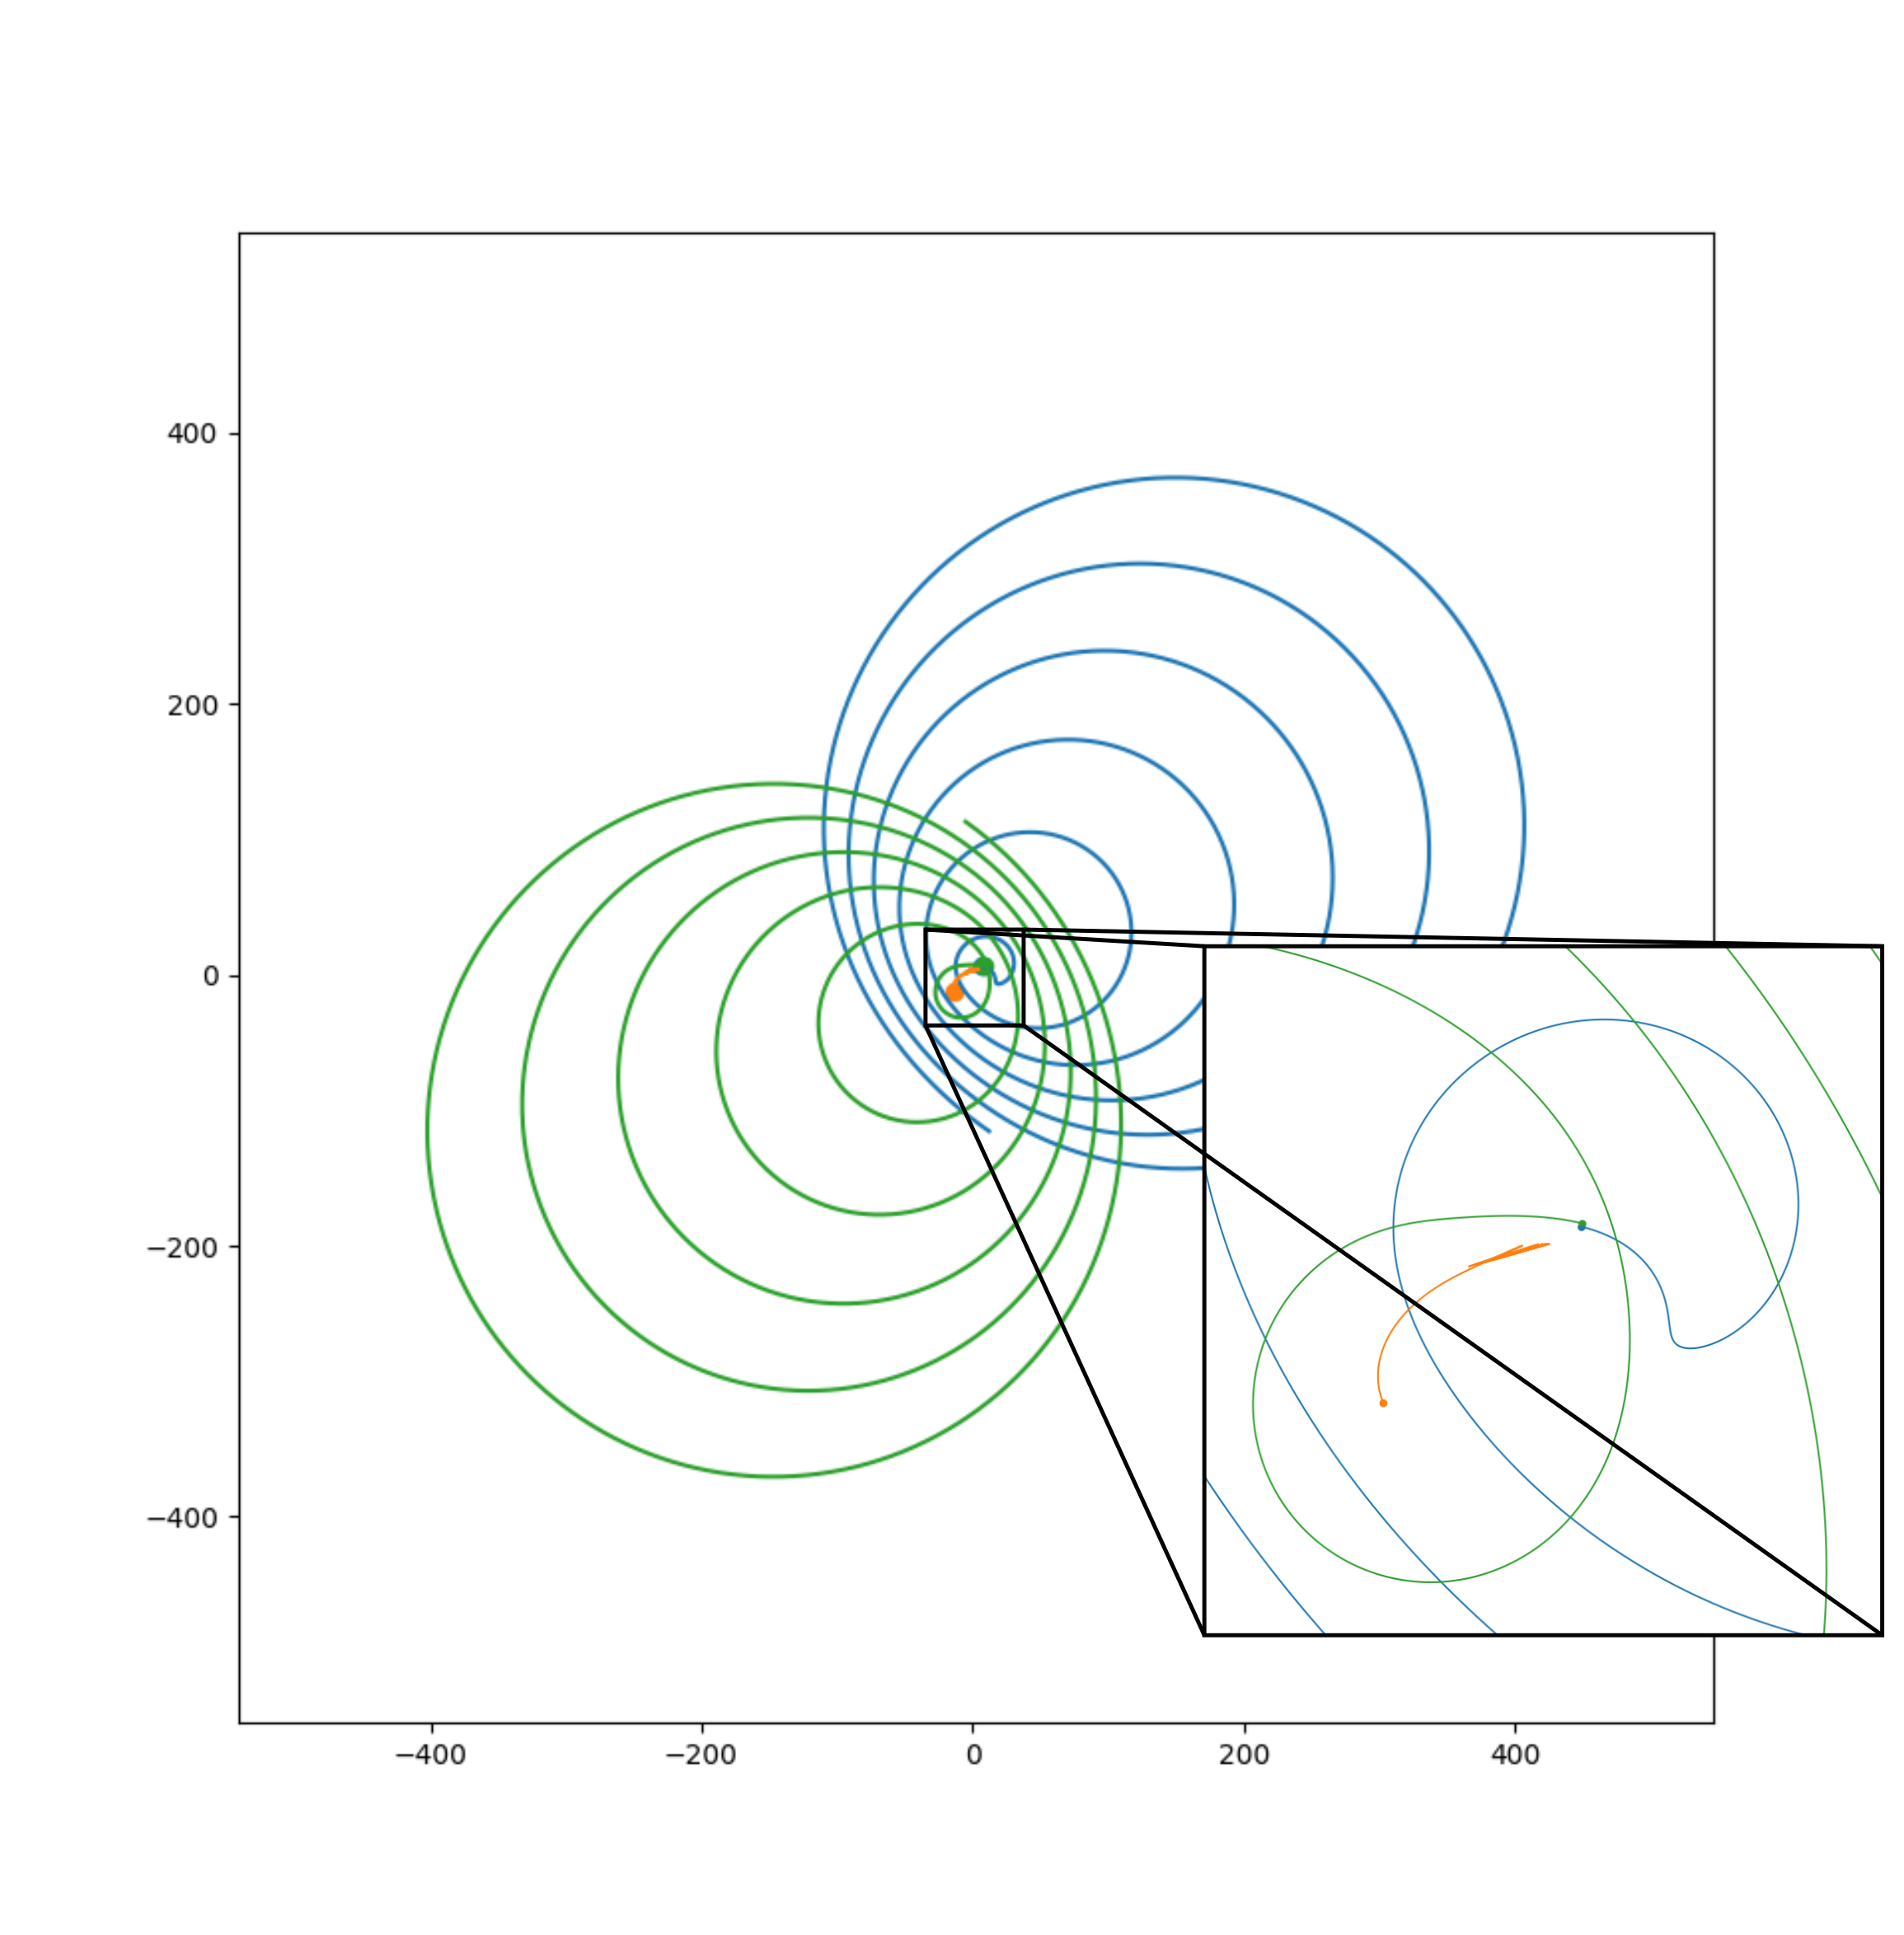
\includegraphics[width=\linewidth]{tcc//img/3corpos_energia0_velocidades_sd_zoom.png}
        \caption{Momentos de forma ($\vet \pi$).}
        \label{fig:3corpos_energia0_velocidades_sd}
    \end{subfigure}
    \caption{Coordenadas objetivas $(\vet \sigma, \vet \pi)$ do problema-modelo \ref{probmodelo:3corpos_energia_nula}.}
    \label{fig:probmodelo3corposenergia0_sd}
\end{figure}

Testamos também o comportamento de um sistema de 3 corpos com energia $E>0$, o problema-modelo \ref{probmodelo:3corpos_energia_positiva}, integrado no intervalo $[4.18,5000]$ via método SVCP8S15 com $h=10^{-4}$ sem correção. O motivo para o instante inicial específico é que o sistema começa com momento de dilatação negativo, e por facilidade foi fixado $h>0$, portanto no intervalo $[0,4.18)$ tem-se $D<0$, o que significa que o ponto de Janus para este caso está na vizinhança de $t=4.18$.

\begin{figure}[H]
    \centering
    \begin{subfigure}{.5\textwidth}
        \centering
        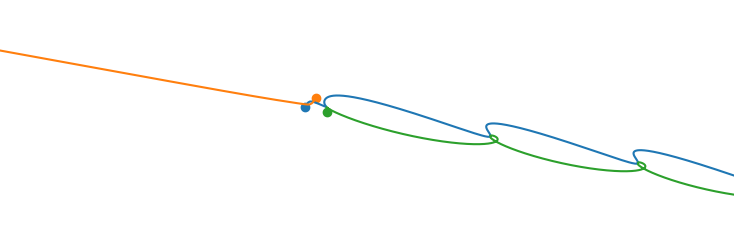
\includegraphics[width=0.8\linewidth]{tcc//img/3corpos_energiapositiva_posicoes_nd.png}
        \caption{}
        \label{fig:3corposenergiapositiva_trajetoria}
    \end{subfigure}%
    \begin{subfigure}{.5\textwidth}
        \centering
        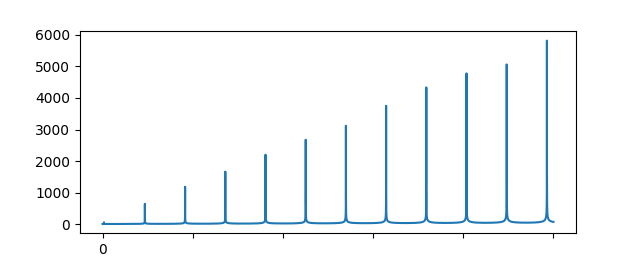
\includegraphics[width=\linewidth]{tcc//img/3corpos_energiapositiva_complexidade.png}
        \caption{}
        \label{fig:3corpos_energiapositiva_complexidade}
    \end{subfigure}
    
    \caption{Problema-modelo \ref{probmodelo:3corpos_energia_positiva}. À esquerda, recorte das trajetórias. À direita, a complexidade apresentada pelo sistema.}
    \label{fig:figuras_probmodel3_energia_positiva}
\end{figure}

Observe que neste problema os picos da complexidade são maiores (figura \ref{fig:3corpos_energiapositiva_complexidade}), refletindo a intensidade das aproximações do sistema binário formado. 

Isso se apresenta também nas coordenadas no espaço de formas. Como no problema com $E=0$, o corpo ejetado desacelera e começa a apresentar um comportamento cíclico e dissipativo (figura \ref{fig:3corpos_energiapositiva_posicoes_sd}). Porém, nesse caso a dissipação é bastante maior que no caso anterior. É visualmente notável a diferença na dissipação observando os momentos (figura \ref{fig:3corpos_energiapositiva_velocidades_sd}), pois o corpo dissipado tem momento oscilando próximo de zero e o sistema binário formado apresenta trajetórias circulares com raios cada vez maiores e com ordem de grandeza $10^5$, enquanto no caso $E=0$ tinha-se ordem de grandeza $10^2$.

\begin{figure}[H]
    \centering
    \begin{subfigure}{.5\textwidth}
        \centering
        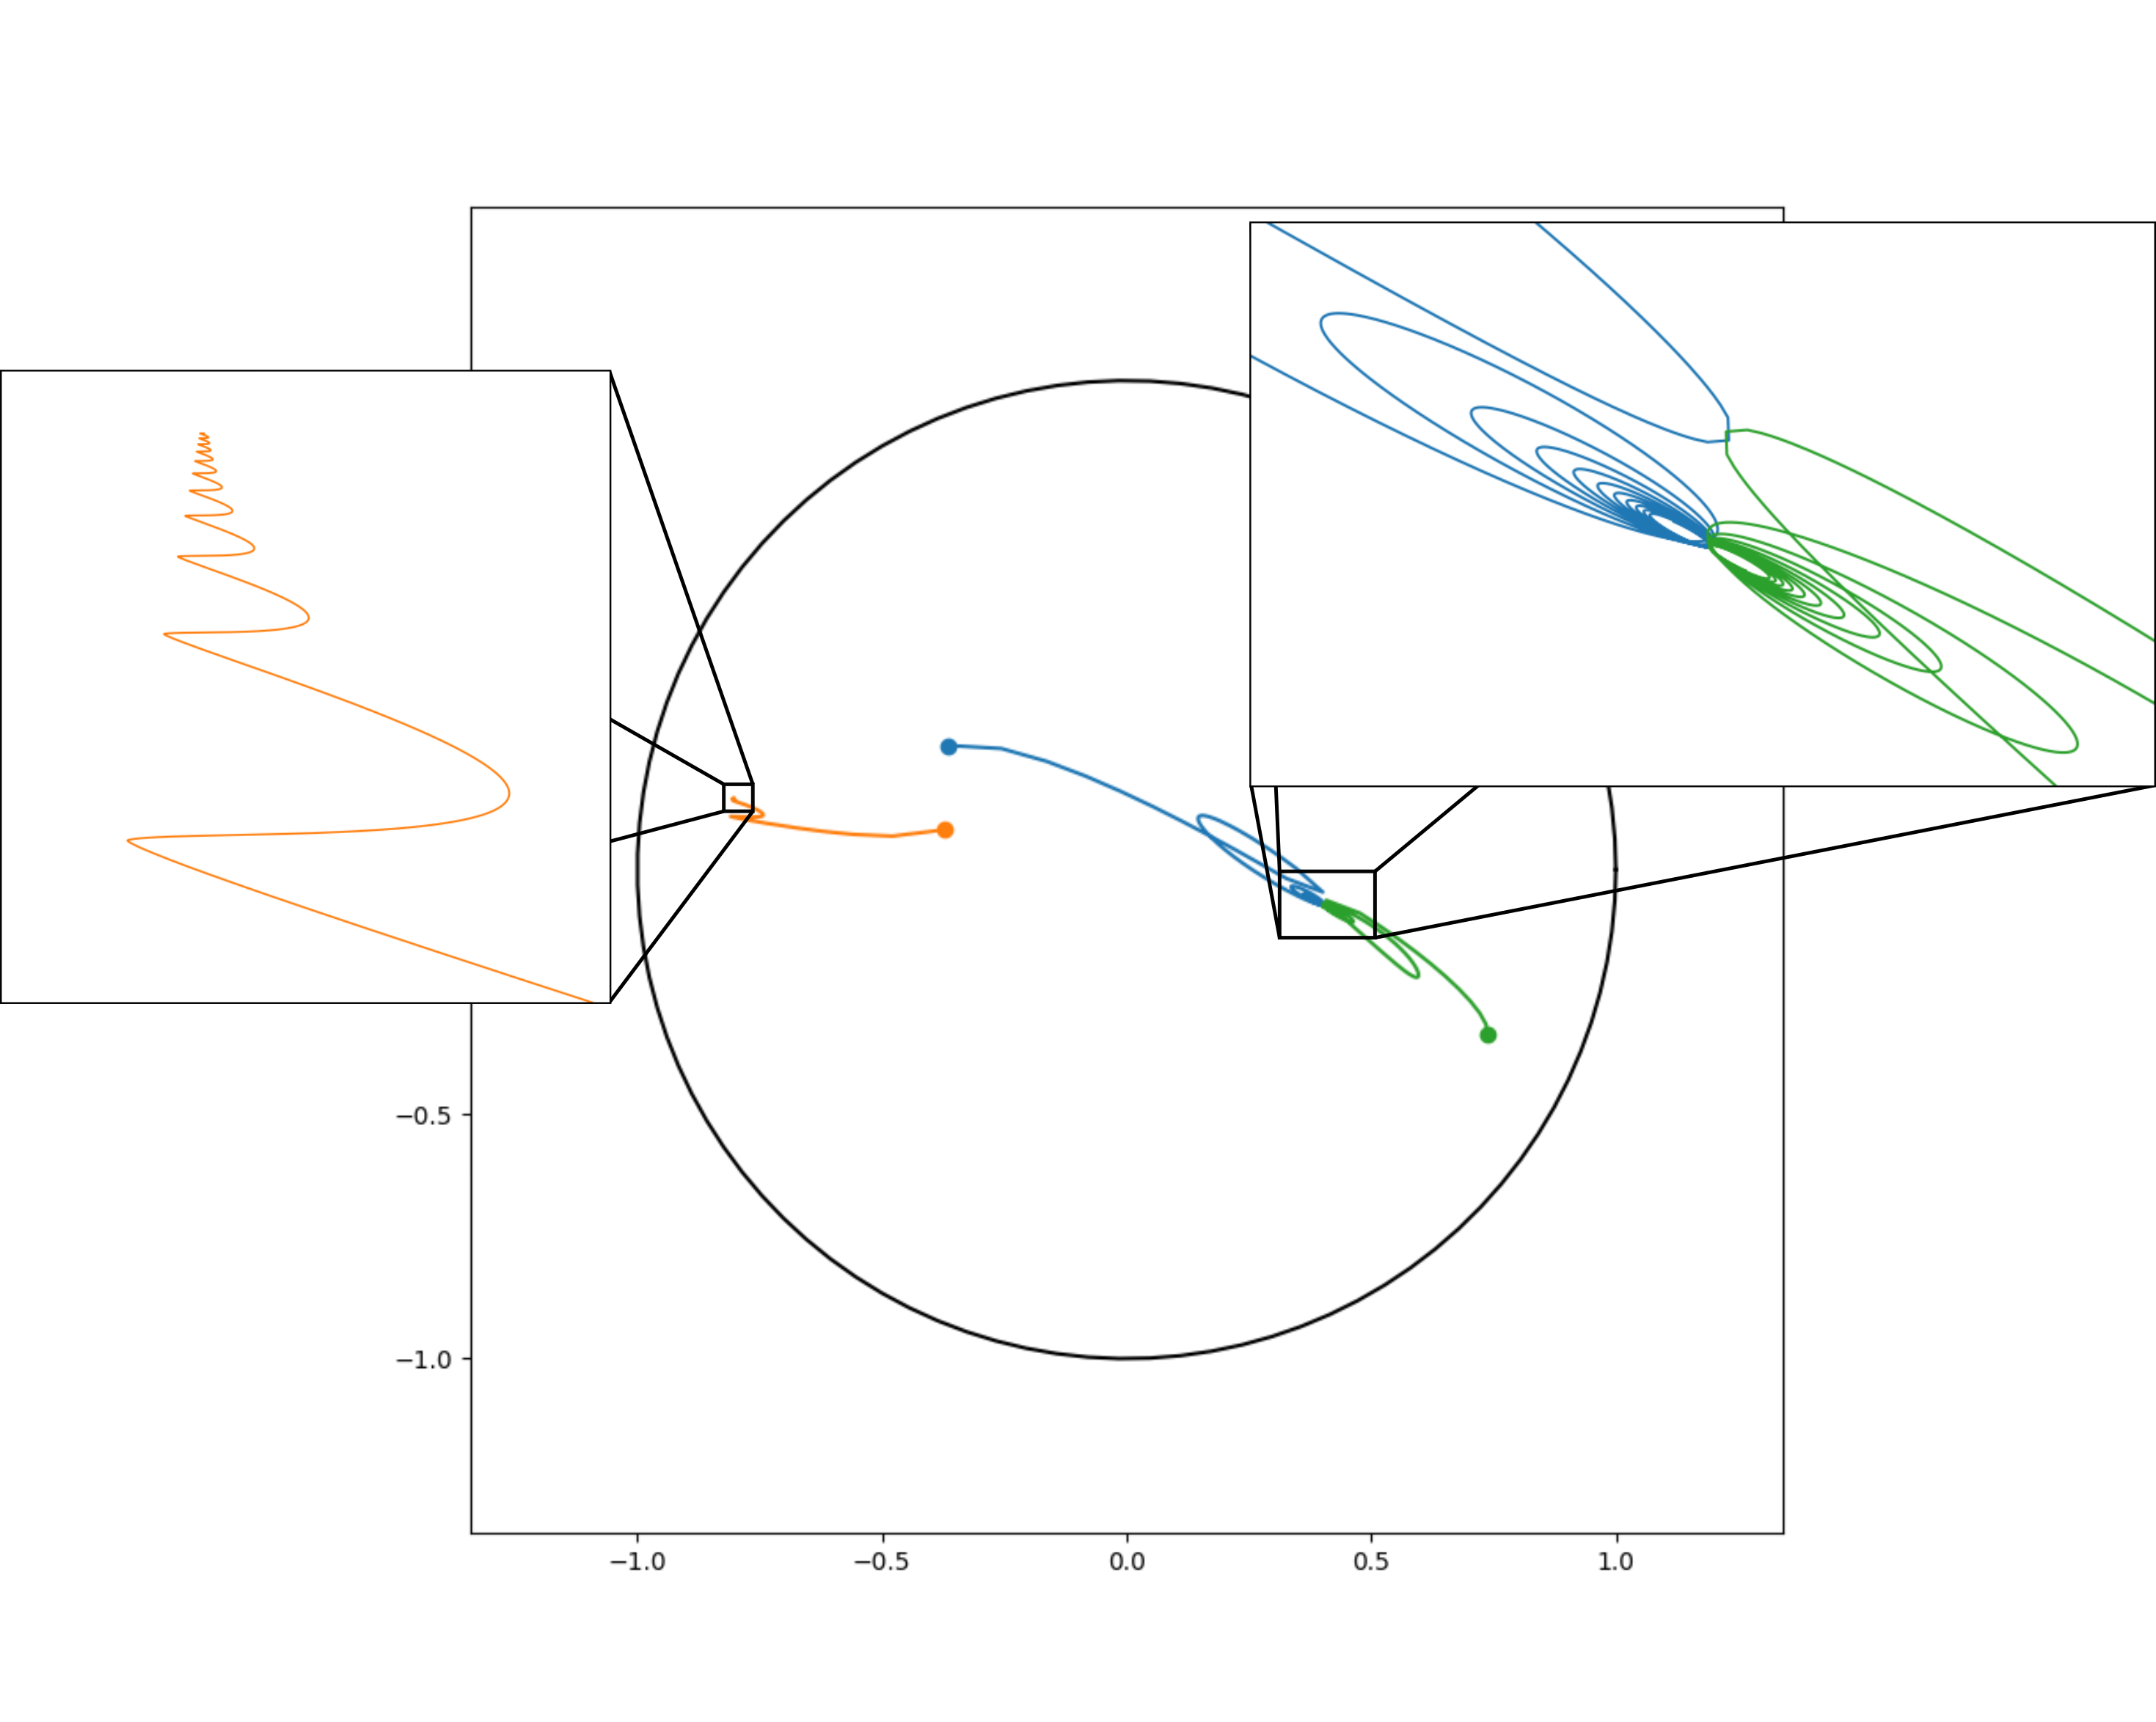
\includegraphics[width=\linewidth]{tcc//img/3corpos_energiapositiva_posicoes_sd_zoom.png}
        \caption{Coordenadas de forma ($\vet \sigma$).}
        \label{fig:3corpos_energiapositiva_posicoes_sd}
    \end{subfigure}%
    \begin{subfigure}{.5\textwidth}
        \centering
        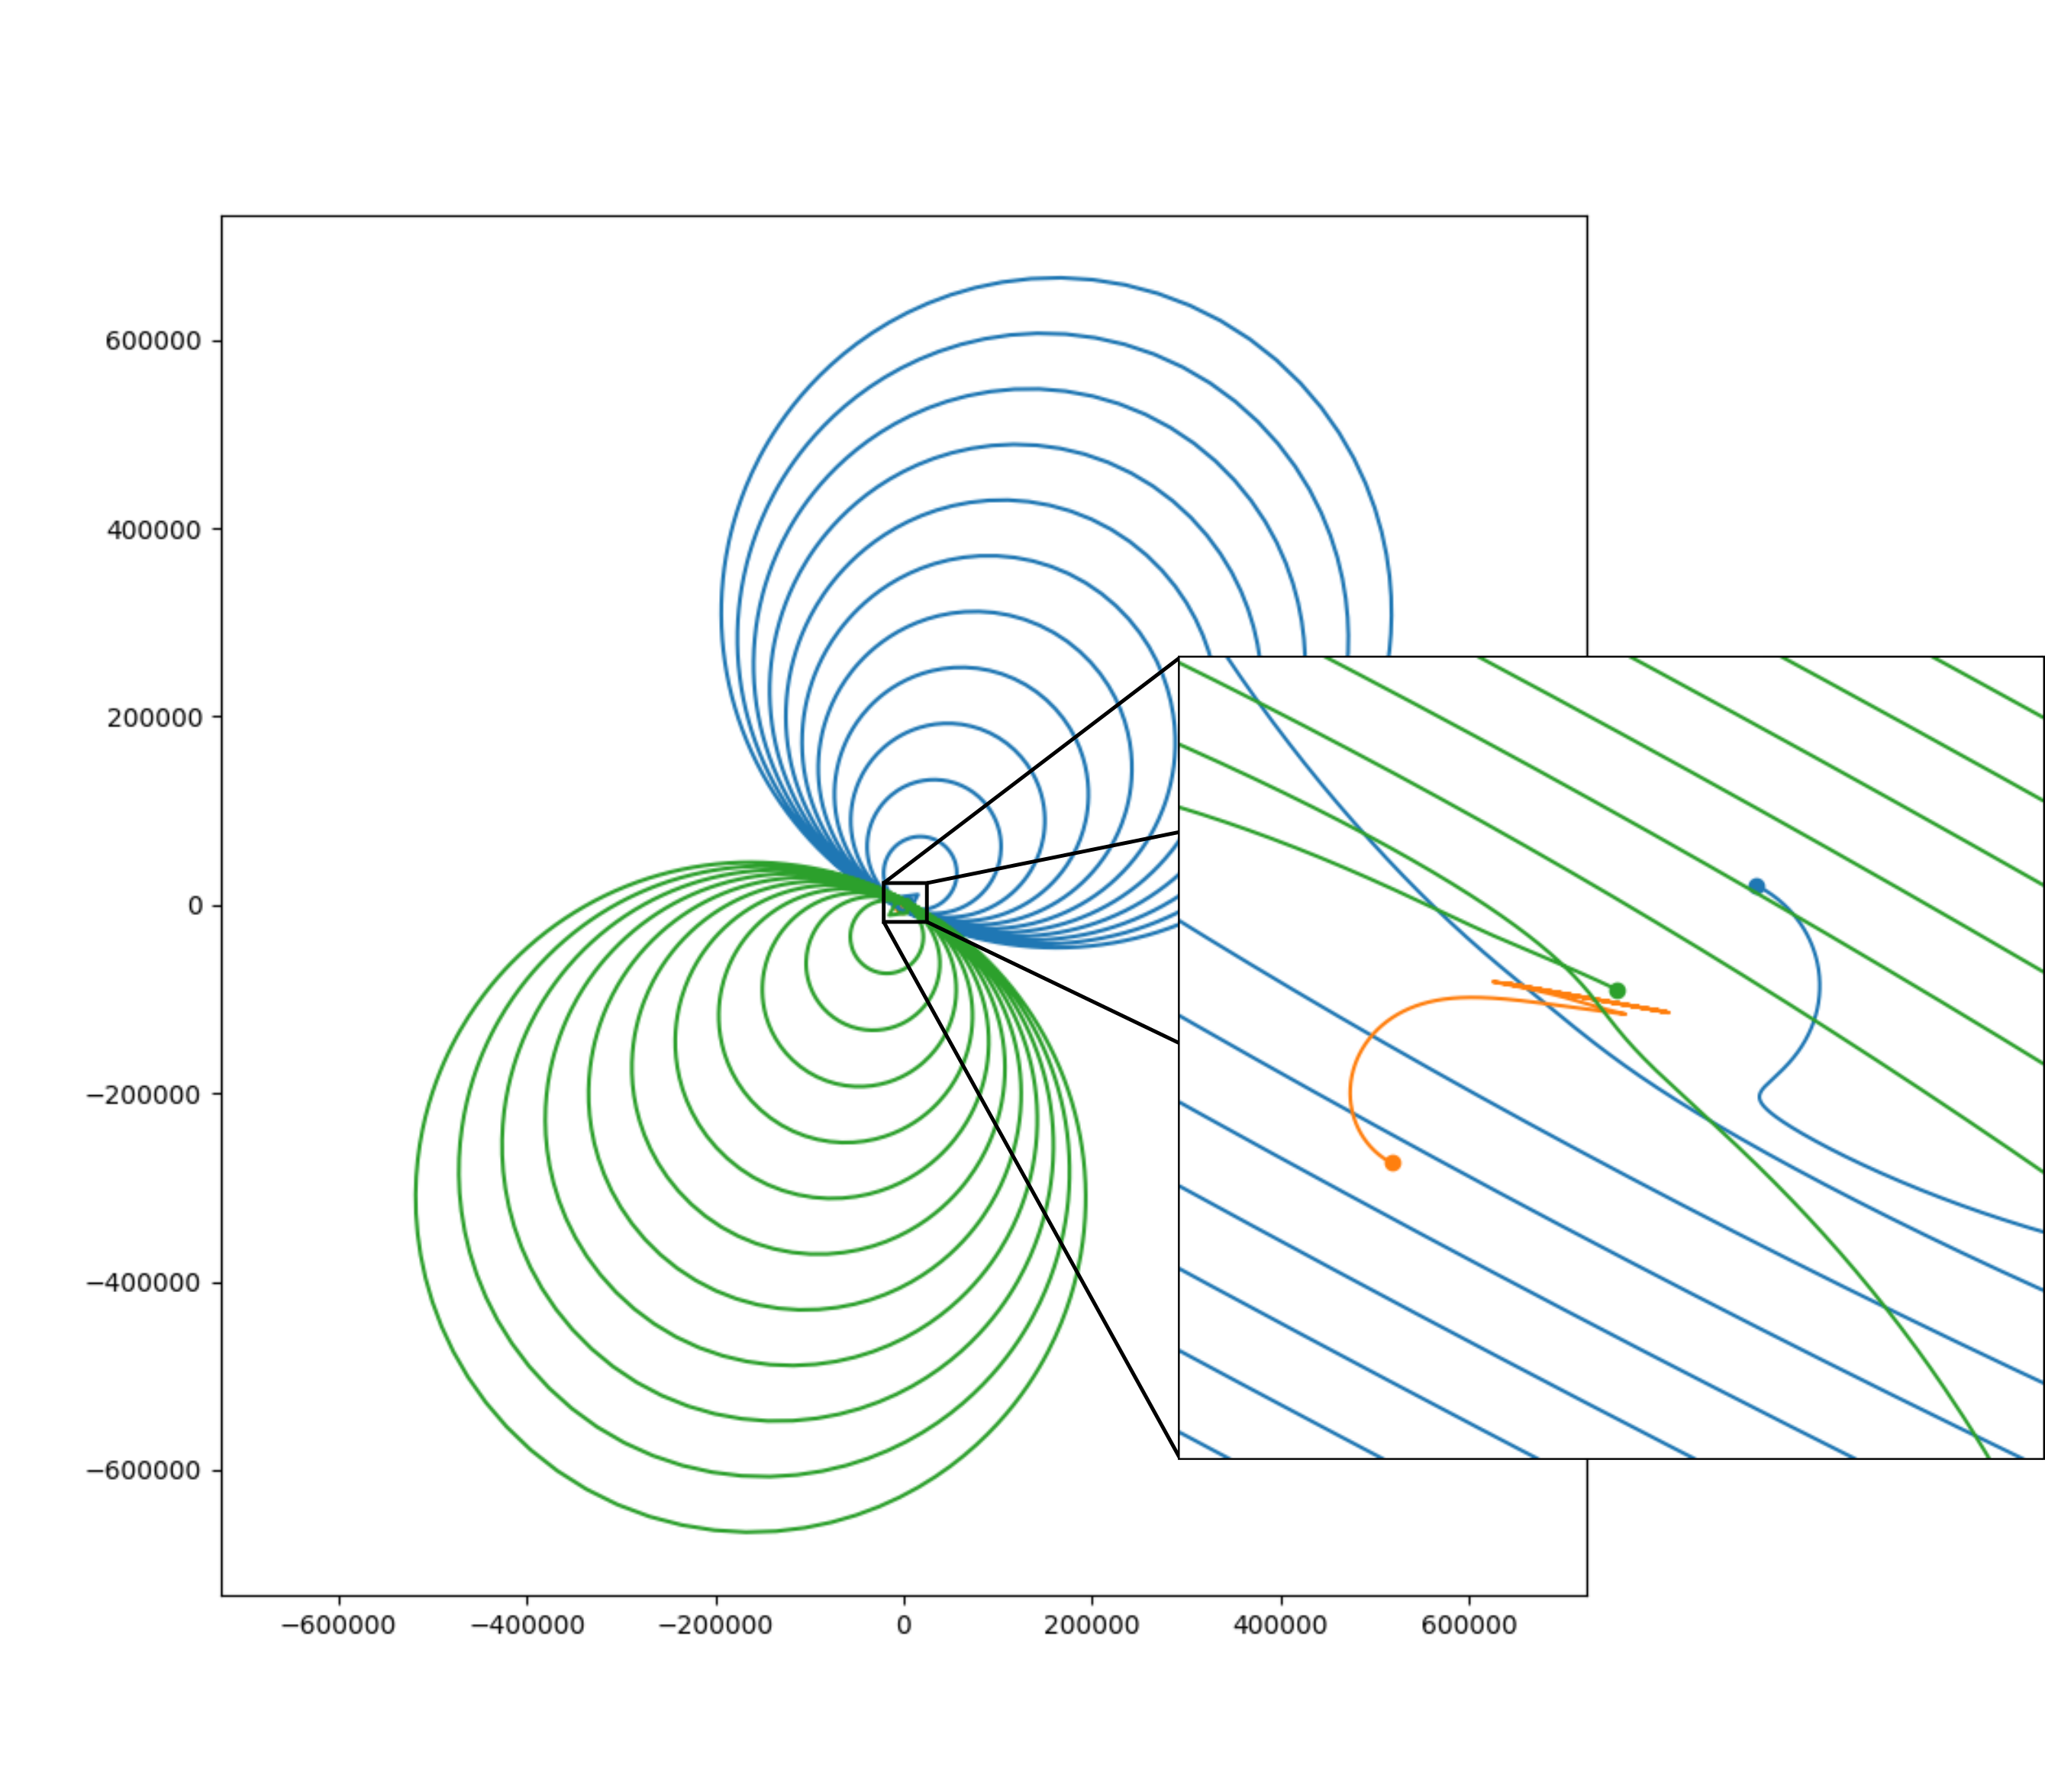
\includegraphics[width=\linewidth]{tcc//img/3corpos_energiapositiva_velocidades_sd_zoom.png}
        \caption{Momentos de forma ($\vet \pi$).}
        \label{fig:3corpos_energiapositiva_velocidades_sd}
    \end{subfigure}
    \caption{Coordenadas objetivas $(\vet \sigma, \vet \pi)$ do problema-modelo \ref{probmodelo:3corpos_energia_positiva}.}
    \label{fig:probmodelo3corposenergiapositiva_sd}
\end{figure}




%%%%%%%% PROBLEMA DE 20 CORPOS
\subsection{Problemas de 20 e 100 corpos}

Para problemas com $N \geq 10$, se mostrou pouco produtivo analisar as trajetórias no espaço de formas devido à quantidade de trajetórias. Além disso, dada a obrigatória separação do sistema em subsistemas em afastamento mútuo, a evolução no tempo newtoniano aumenta o momento de inércia $R^2$ mais rapidamente que o afastamento entre os corpos, levando as trajetórias no centro da esfera unitária a esferas cada vez menores e os corpos distantes a desacelerarem em algum ponto da esfera. 

\begin{figure}
    \centering
    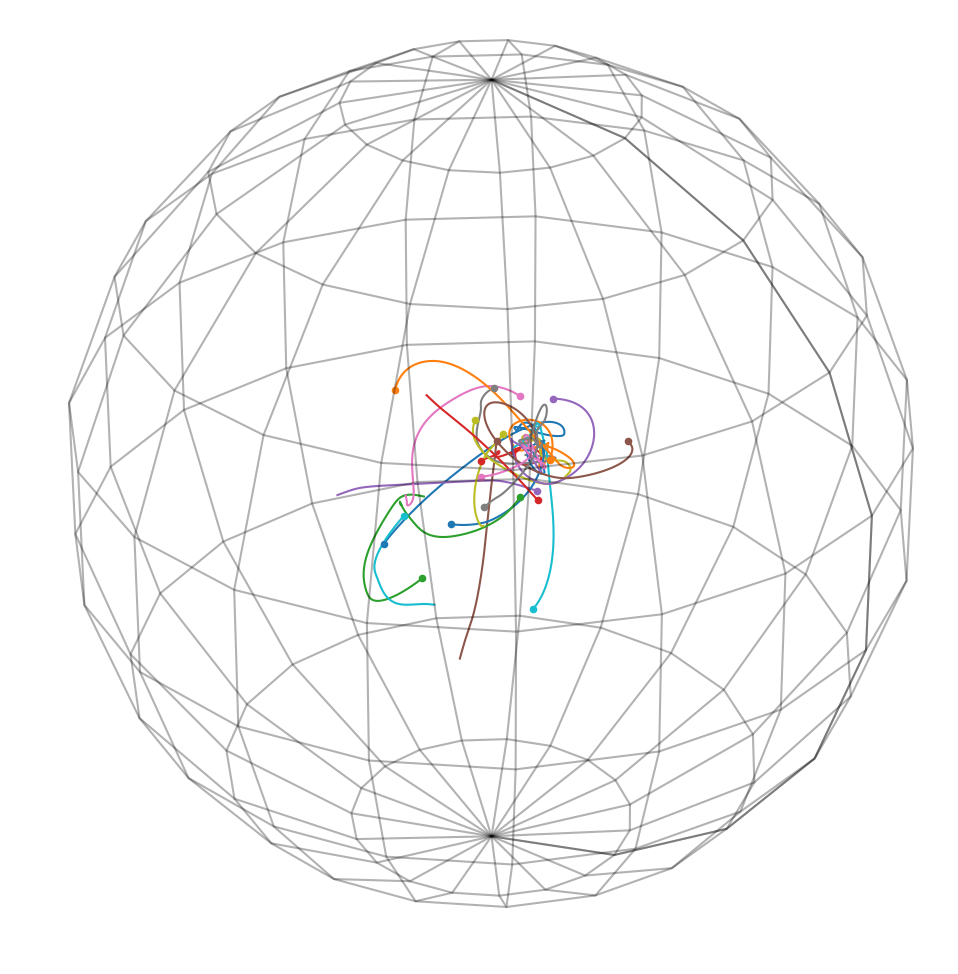
\includegraphics[width=0.5\linewidth]{tcc//img/20corpos_energia0_posicoes_3d_sd.png}
    \caption{Trajetória objetiva do problema-modelo \ref{probmodelo:20corpos_energia0}.}
    \label{fig:20corpos_trajetorias_sd}
\end{figure}

Para visualizar esse comportamento, simulamos o problema-modelo \ref{probmodelo:20corpos_energia0} com 20 corpos no intervalo $[0,5000]$ via RKN671 com $h=10^{-2}$ e $\epsilon=8h$. Nesse problema, todas as integrais primeiras são nulas. A trajetória objetiva pode ser visualizada na figura \ref{fig:20corpos_trajetorias_sd}.

A complexidade (figura \ref{fig:20corpos_complexidade}), porém, para $N=20$ já apresenta mais nitidamente o comportamento esperado: a expansão do sistema (grande escala) faz com que $C_S$ cresça no tempo newtoniano, e as interações entre os subsistemas (pequena escala) se apresentam nas variações desse crescimento, bastante nítidas nos casos de aproximações intensas facilmente identificáveis pelos maiores picos de $C_S$.

\begin{figure}[H]
    \centering
    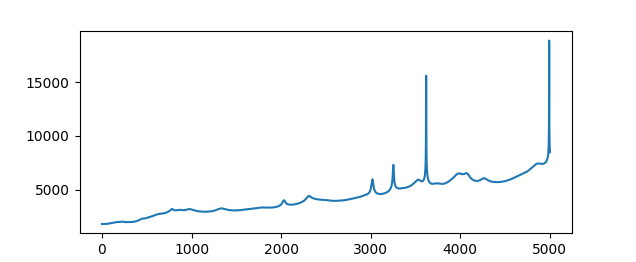
\includegraphics[width=0.8\linewidth]{tcc//img/20corpos_energia0_complexidade.png}
    \caption{Complexidade do problema-modelo \ref{probmodelo:20corpos_energia0}.}
    \label{fig:20corpos_complexidade}
\end{figure}

Simulamos também um problema de 100 corpos com todas as integrais primeiras nulas (\ref{probmodelo:100corpos_energia0}) no intervalo $[-10^6,10^6]$ via método de Verlet com $h=0.04=\epsilon$ em paralelo. Vale ressaltar que a simulação levou cerca de 108 segundos.

Na figura \ref{fig:100corpos_complexidade} podemos observar como as propriedades da complexidade se mostram ainda mais nítidas que no caso $N=20$. Além disso, como foi feita também a integração para o passado, é possível visualizar o ponto de Janus (o mínimo de $C_S$). Nesse caso, dada a grande variação de $C_S$, é possível observar que o sistema não apresentou grande expansão num primeiro momento, mas uma quantidade grande de interações no centro de massas.

\begin{figure}
    \centering
    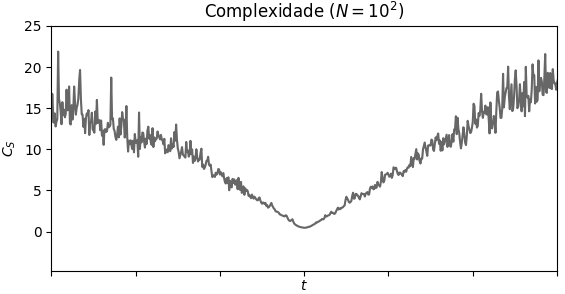
\includegraphics[width=0.6\linewidth]{tcc//img/complexidade100.png}
    \caption{Complexidade do problema-modelo \ref{probmodelo:100corpos_energia0}.}
    \label{fig:100corpos_complexidade}
\end{figure}


%%%%%%%% PROBLEMA DE 1000 CORPOS
\subsection{Problemas de 1000 corpos}

Passando para escalas maiores, realizamos três simulações com $N=10^3$ no intervalo $[-10^4, 10^4]$ via método de Verlet com $h=0.04=\epsilon=h$ para observar o comportamento de $C_S$ com diferentes valores de $E$: $-0.25$, $0$ e $0.25$.


\subsubsection{Energia total nula}

Começando pelos casos nos quais temos informações esperadas sobre o comportamento, o problema-modelo \ref{probmodelo:1000corpos_energianula} contém as condições iniciais para $E=0$ (todas as integrais primeiras são nulas, na verdade). Na figura \ref{fig:1000corpos_energia0_complexidade} é possível observar o crescimento variado de $C_S$ de maneira semelhante em relação ao eixo definido pelo Ponto de Janus. A vizinhança desse instante se apresentou nesse caso como um momento de rápida expansão e intensas aproximações, seguido pelo início de um momento de maior estabilidade tanto dos corpos ejetados quanto dos corpos ainda próximos ao centro. 

\begin{figure}[H]
    \centering
    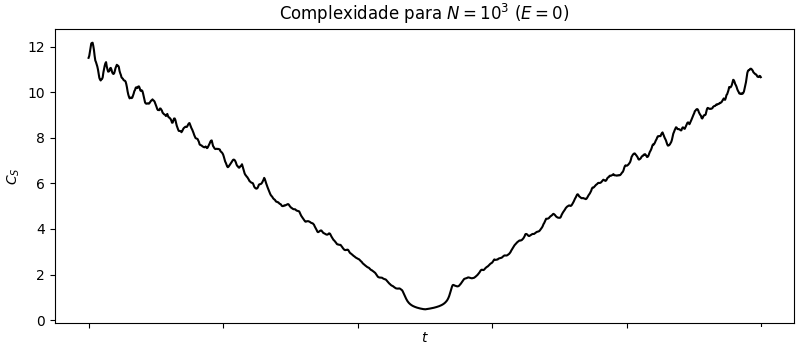
\includegraphics[width=0.6\linewidth]{tcc//img/complexidade_1000_nula.png}
    \caption{Complexidade do problema-modelo \ref{probmodelo:1000corpos_energianula}.}
    \label{fig:1000corpos_energia0_complexidade}
\end{figure}

A evolução do sistema pode ser observada na figura \ref{fig:1000corpos_energia0_posicoes}. O centro de massas concentra grande parte dos corpos mesmo nos limites do intervalo considerado, mas a ejeção de partículas continua acontecendo.

\begin{figure}[H]
    \centering
    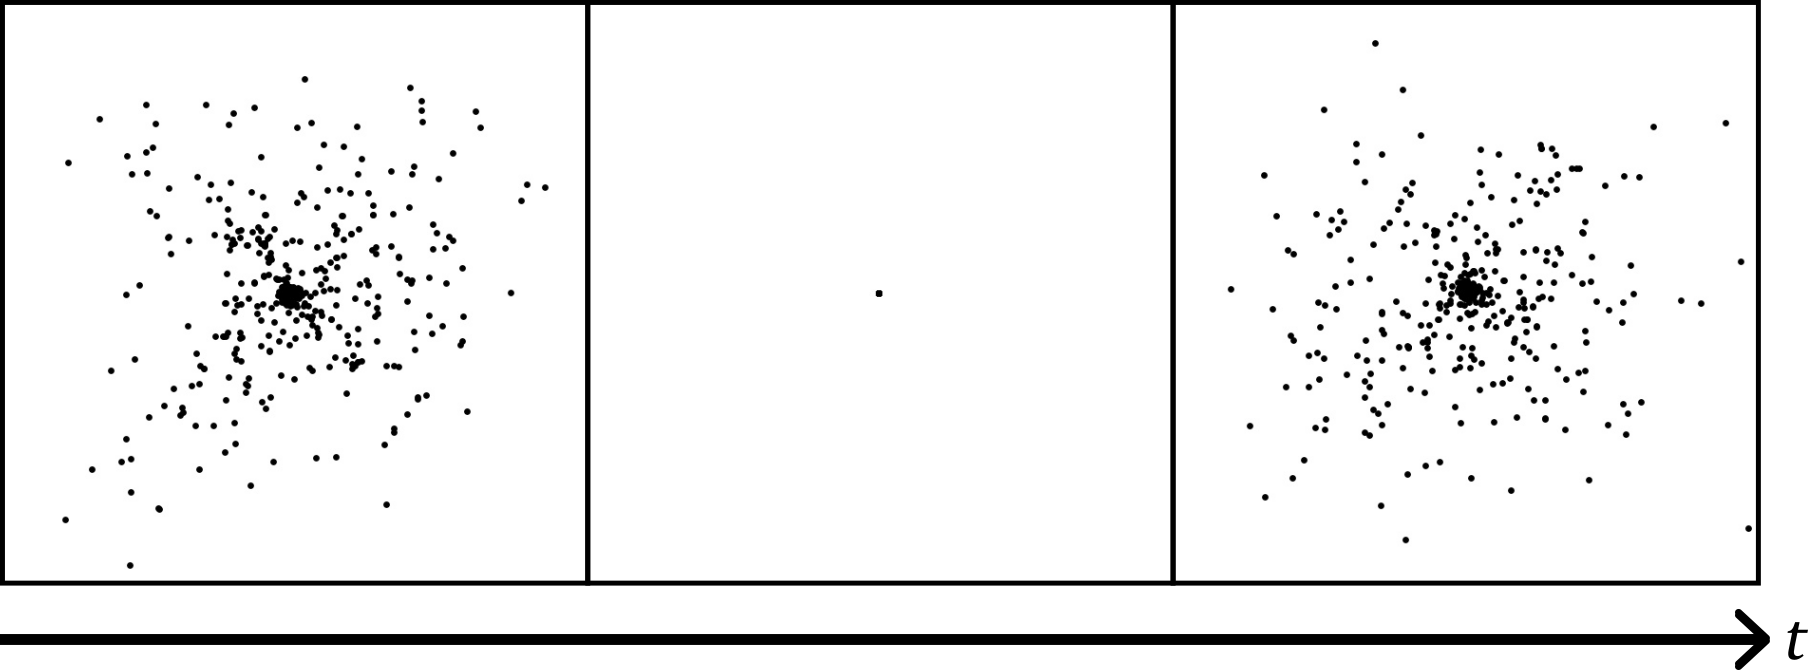
\includegraphics[width=0.8\linewidth]{tcc//img/espalhamento_energia_nula_1000.png}
    \caption{Instantes do bordo e $t=0$ do problema-modelo \ref{probmodelo:1000corpos_energianula}.}
    \label{fig:1000corpos_energia0_posicoes}
\end{figure}


\subsubsection{Energia total positiva}
Já para o caso $E=0.25$ no problema-modelo \ref{probmodelo:1000corpos_energiapositiva_1}, com massas $m=1/N$, observamos uma baixa variação de $C_S$ (figura \ref{fig:1000corpos_energiapositiva_complexidade_1}). Como o sistema necessariamente se contrai e se expande (devido ao comportamento do momento de inércia previsto pela relação de Lagrange-Jacobi), isso indica que a interação gravitacional entre os corpos é quase inversamente proporcional ao tamanho do sistema, o que sugere a não formação de binários e, do ponto de vista da do espaço de formas, o resultado é o esperado: o sistema assintoticamente congela.

\begin{figure}[H]
    \centering
    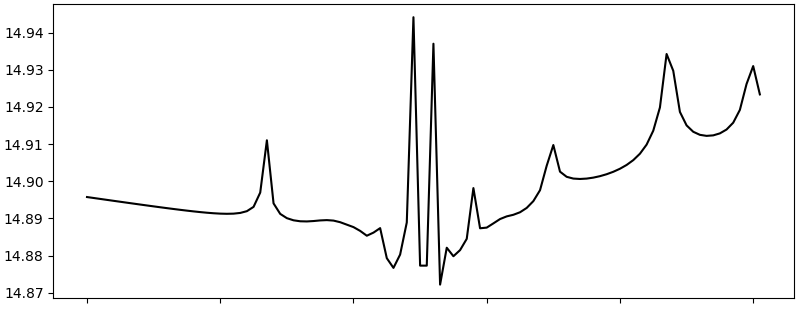
\includegraphics[width=0.6\linewidth]{tcc//img/1000corpos_energiapositiva_complexidade_1.png}
    \caption{Complexidade do problema-modelo \ref{probmodelo:1000corpos_energiapositiva_1}.}
    \label{fig:1000corpos_energiapositiva_complexidade_1}
\end{figure}

Na figura \ref{fig:1000corpos_energiapositiva_posicoes_1} é possível observar um espalhamento bastante uniforme dos corpos no espaço. Uma vez que os valores iniciais foram gerados através de uma distribuição uniforme, isso reflete o baixo nível de interação entre os corpos.

\begin{figure}[H]
    \centering
    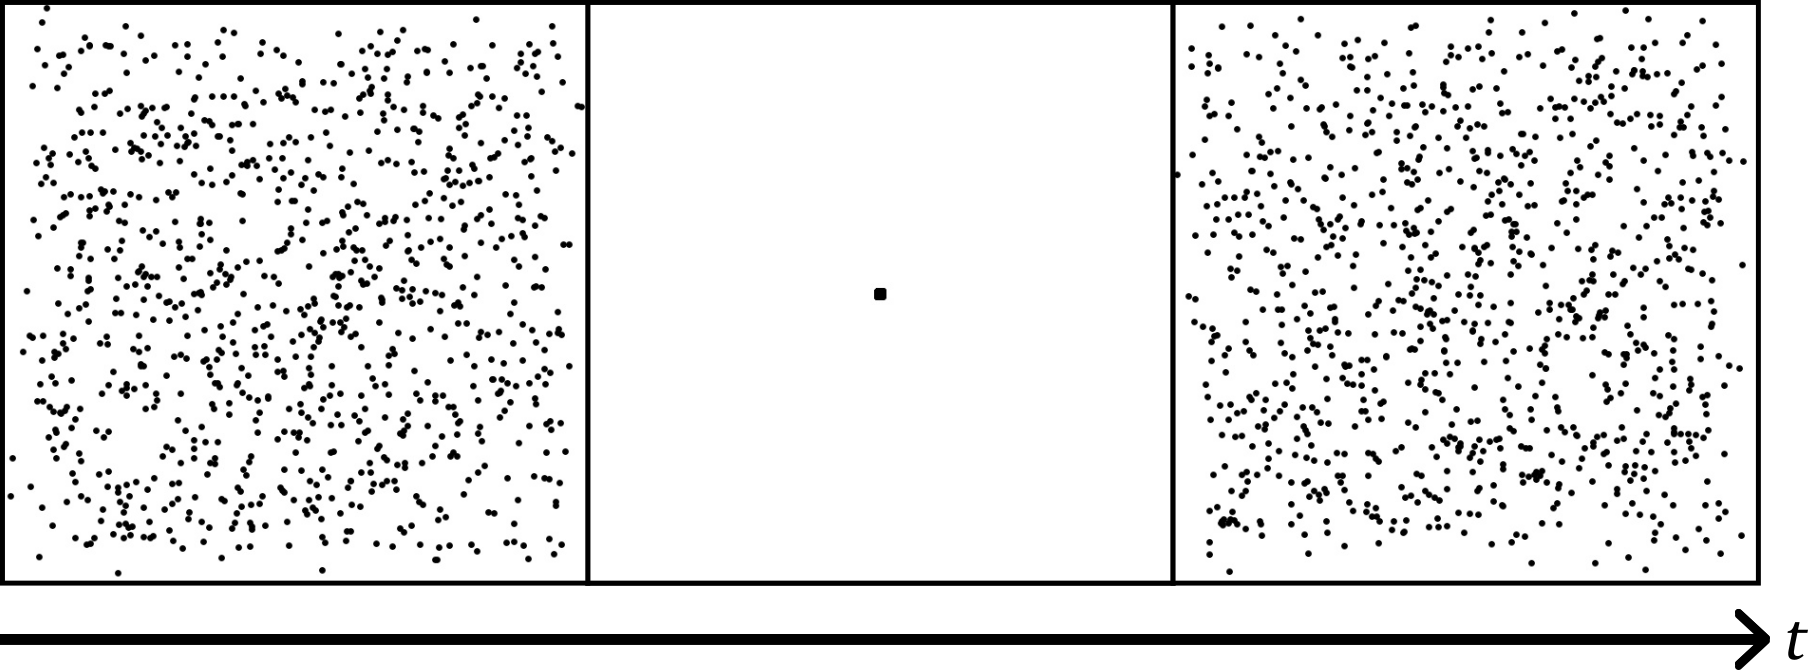
\includegraphics[width=0.8\linewidth]{tcc//img/espalhamento_energia_positiva_1000.png}
    \caption{Instantes do bordo e $t=0$ do problema-modelo \ref{probmodelo:1000corpos_energiapositiva_1}.}
    \label{fig:1000corpos_energiapositiva_posicoes_1}
\end{figure}


Optamos então por gerar novos valores iniciais mas com massas um pouco maiores individualmente, mas o suficiente para o sistema aumentar $10^3$ vezes em massa total (problema-modelo \ref{probmodelo:1000corpos_energiapositiva_2}). Nesse caso, o problema apresentou um comportamento mais parecido com o caso $E=0$, pois as interações gravitacionais foram mais intensas (veja figura \ref{fig:1000corpos_energiapositiva_posicoes_2}).

\begin{figure}[H]
    \centering
    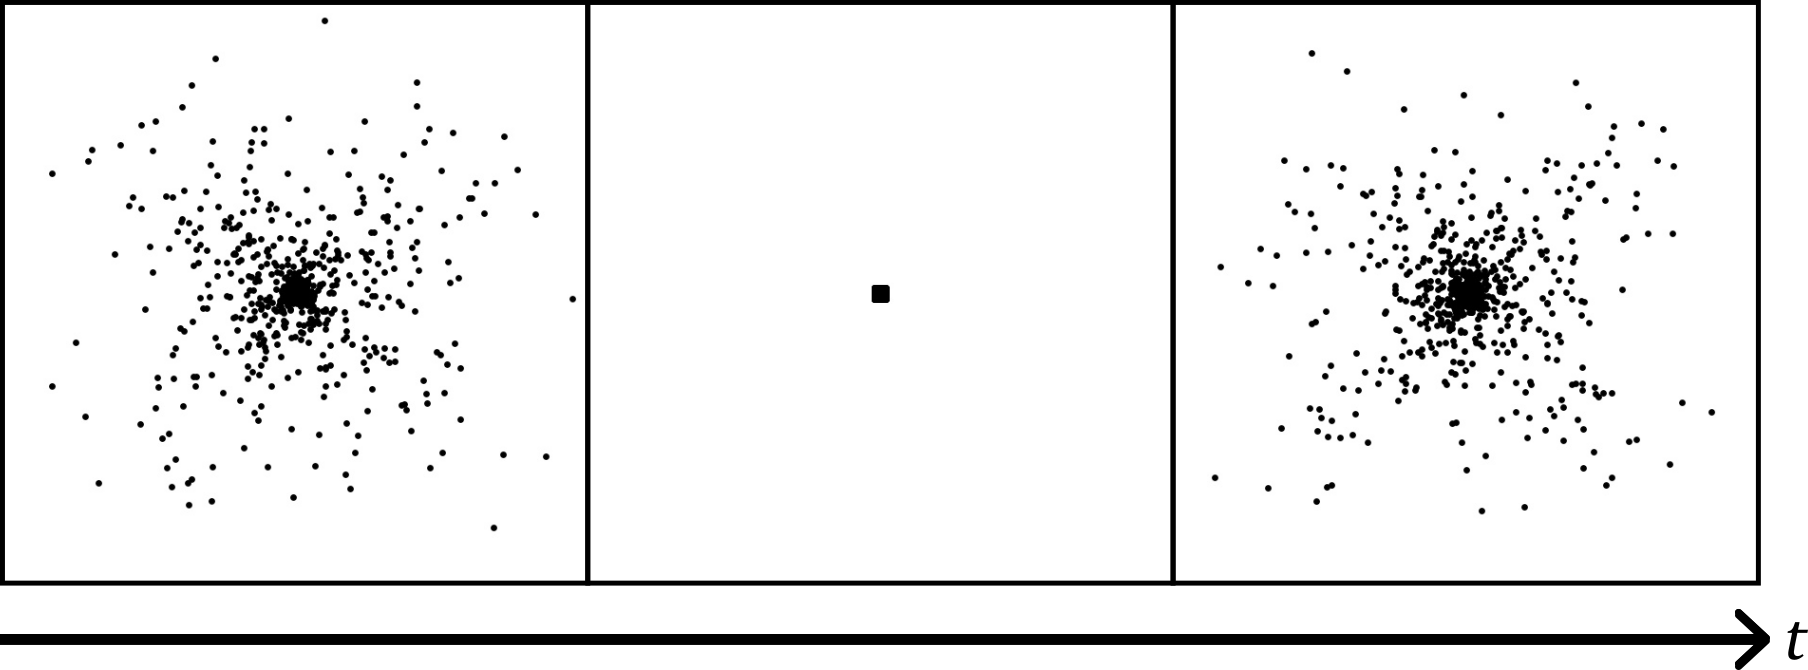
\includegraphics[width=0.8\linewidth]{tcc//img/espalhamento_energia_positiva_1000_2.png}
    \caption{Instantes do bordo e $t=0$ do problema-modelo \ref{probmodelo:1000corpos_energiapositiva_2}.}
    \label{fig:1000corpos_energiapositiva_posicoes_2}
\end{figure}

A complexidade também apresentou um comportamento diferente do primeiro exemplo de $E=0.25$ com um formato semelhante ao de $E=0$, mas com uma grande diferença de escala (veja figura \ref{fig:1000corpos_energiapositiva_complexidade_2}).

\begin{figure}
    \centering
    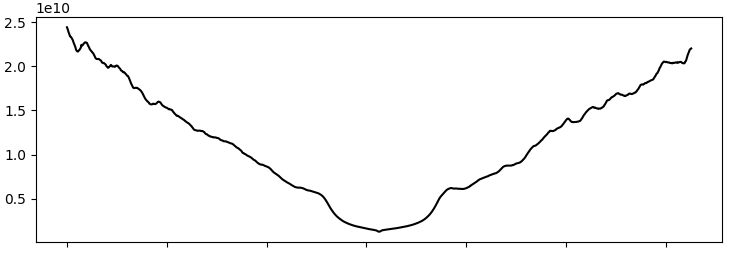
\includegraphics[width=0.8\linewidth]{tcc//img/1000corpos_energiapositiva_complexidade_2.png}
    \caption{Complexidade no problema-modelo \ref{probmodelo:1000corpos_energiapositiva_2}.}
    \label{fig:1000corpos_energiapositiva_complexidade_2}
\end{figure}


\subsubsection{Energia total negativa}
Por fim, no caso $E=-0.25$ tivemos um resultado curioso. Embora as condições impostas inicialmente tenham sido as de Hénon (veja subseção \ref{subsection:condicoes_aarseth}), a complexidade apresentou um comportamento de cúspide (figura \ref{fig:1000corpos_energianegativa_complexidade}. O que ocorre é que na evolução do sistema nesse caso são ejetados alguns corpos (o que provoca o crescimento) mas mantém relativa estabilidade no centro de massas.

\begin{figure}[H]
    \centering
    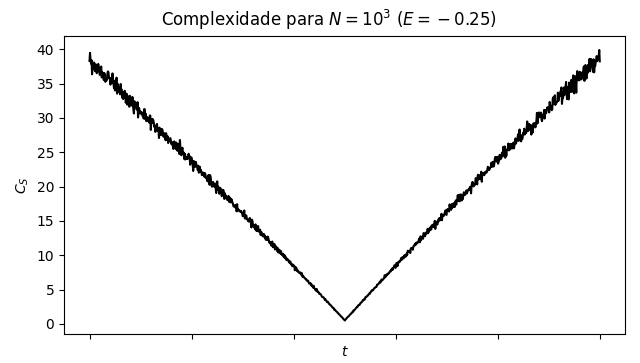
\includegraphics[width=0.6\linewidth]{tcc//img/complexidade1000_energianegativa.png}
    \caption{Complexidade no problema-modelo \ref{probmodelo:1000corpos_energianegativa}.}
    \label{fig:1000corpos_energianegativa_complexidade}
\end{figure}

Esse comportamento pode ser observado na figura \ref{fig:1000corpos_energianegativa_posicoes}, onde a maior parte do sistema fica contida na região central enquanto alguns poucos corpos são ejetados, sem formação de binários.

\begin{figure}[H]
    \centering
    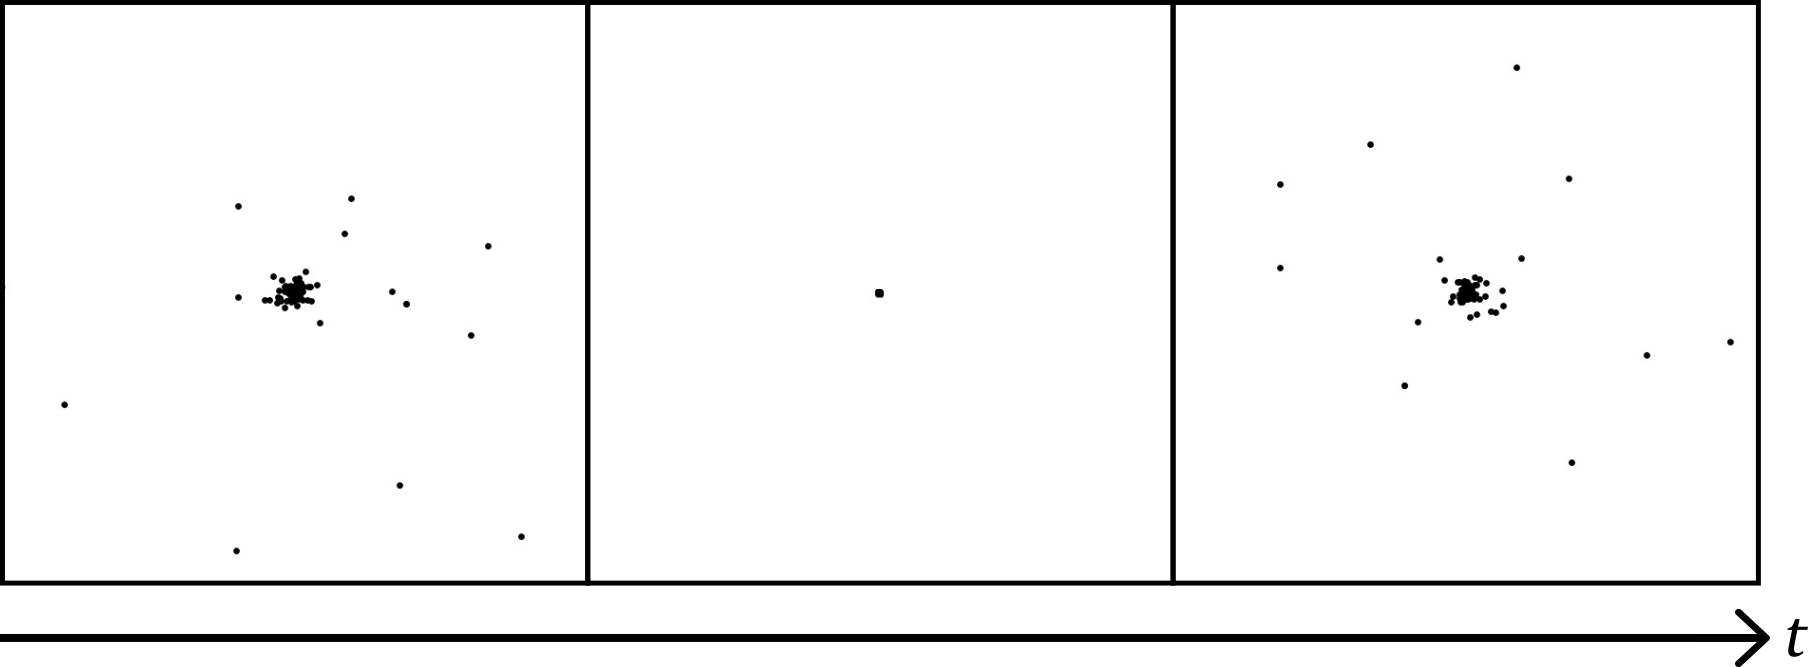
\includegraphics[width=0.8\linewidth]{tcc//img/espalhamento_energia_negativa_1000.png}
    \caption{Instantes do bordo e $t=0$ do problema-modelo \ref{probmodelo:1000corpos_energianegativa}.}
    \label{fig:1000corpos_energianegativa_posicoes}
\end{figure}

Na vizinhança do Ponto de Janus, porém, é possível encontrar semelhanças com os casos $E \geq 0$, como na formação de um pequeno ``vale'' a princípio seguido do início da variação (figura \ref{fig:1000corpos_energianegativa_complexidade_zoom}).

\begin{figure}[H]
    \centering
    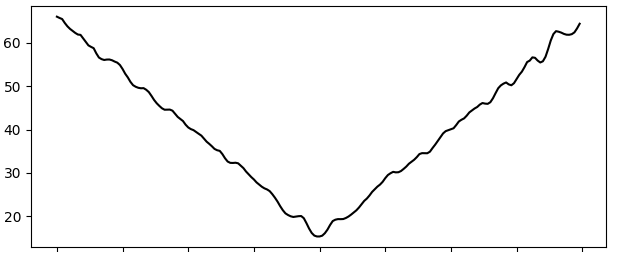
\includegraphics[width=0.8\linewidth]{tcc/img/zoom_complexidade_1000corpos_negativa.png}
    \caption{Vizinhança do ponto de Janus no problema $N=10^3$ com $E=-0.25$.}
    \label{fig:1000corpos_energianegativa_complexidade_zoom}
\end{figure}

% * TESTES PRATICOS E PROGRAMA FINAL
%    
%   Fazer alguns testes legais e apresentar como o programa 
%   ficou no final.
%   ????
\chapter{Conclusão}

Apresentamos neste trabalho algumas formas de simular numericamente o Problema de N-Corpos Gravitacional. Ainda que mal tenhamos saído da superfície na área de simulações numéricas, obtivemos alguns resultados.

Para começar, o PNCG é um problema mecânico ideal para um primeiro mas dedicado estudo de métodos numéricos. Sua instabilidade numérica e todas as dificuldades técnicas apresentadas, como o custo computacional e as colisões, necessitam de atenção e estimulam a criatividade matemática continuamente.

Qualitativamente, o capítulo \ref{capitulo:metodos_numericos} mostra nitidamente a superioridade das aproximações numéricas dos integradores simpléticos, especialmente para integrações em larga escala, demonstrando a solidez da Mecânica Hamiltoniana esperada no capítulo \ref{capitulo:revisao_mecanica}. Vale ressaltar que muita teoria já existe a respeito dos métodos simpléticos, inclusive sobre sua estabilidade através da teoria de Kolmogorov-Arnold-Moser (KAM), e trata-se de uma área em ativo desenvolvimento a qual merece atenção.

Além disso, existem muitas outras formas de integração numérica que não foram tratadas, como os métodos implícitos, os com controle automático de tamanho de passo e os métodos de passo múltiplo. Para o PNCG em específico, existem esquemas de passo múltiplo utilizados na literatura que demonstram um bom desempenho para simulações astrofísicas e cosmológicas, como apresenta \cite{aarseth_gravitational_2003}.

Também vimos que o corretor numérico se mostrou aplicável e que corrigir somente a energia é suficiente, embora não tenha sido possível testá-lo em larga escala. Pretendemos simular problemas com valores de $N$ maiores e em escalas de tempo mais longas que as aqui apresentadas para entender melhor a confiabilidade da correção.

Quanto às colisões elásticas, também não foi possível neste tempo fazer testes em larga escala para intuir sobre sua aplicabilidade, mas é uma alternativa com potencial. Quanto ao amortecimento, o uso de diferentes valores de $\epsilon$ em diferentes simulações neste trabalho que ainda assim validavam os resultados teóricos esperados indicam a pouca influência de um $\epsilon$ suficientemente pequeno sobre os resultados qualitativos do sistema como um todo, apesar da diferença nas trajetórias individuais.

O método apresentado para gerar valores iniciais se mostrou enviesado. Isso se reflete na dramática diferença entre utilizar massas $m=1/N$ e massas $m>1$ nas simulações com $E>0$ vistas na seção \ref{secao:simulacao_dinamica_de_formas}. De fato, cabe um maior estudo sobre a geração de valores iniciais para o PNCG e a devida escolha de parâmetros de modo que seja possível extrair resultados mais gerais das simulações.

Quanto ao programa desenvolvido, disponível em \href{https://github.com/potalej/gravidade-fortran}{https://github.com/potalej/gravidade-fortran} \citep{potalej_gravidade-fortran}, este se mostrou bem-sucedido nas simulações embora com um custo computacional relativamente expressivo. As simulações de $N=10^3$ para grandes intervalos de futuro e passado levaram cerca de 20 minutos quando se habilitava a paralelização no \textit{hardware} disponível, gerando arquivos consideravelmente grandes e de custosa análise via Python. O uso de GPUs (\textit{Graphics Processing Unit}, unidades de processamento gráfico) é um caminho possível a se seguir para diminuir o tempo das simulações, mas não tivemos a possibilidade de testá-lo até o momento.

Pudemos também visualizar os resultados fornecidos pela Dinâmica de Formas quanto às setas do tempo. A complexidade é uma forma interessante de resumir o comportamento do sistema como um todo, e também pode ser um indicador da estabilidade de um sistema de $N$-corpos para valores de $E < 0$ ainda não totalmente explorados.

Em suma, a simulação numérica do Problema de N-Corpos Gravitacional é uma área matematicamente rica e profunda, e os resultados deste trabalho, como apresentado nesta seção, trouxeram ainda mais questões e novas possibilidades do que respostas. Há muitos caminhos a seguir, e simular numericamente o PNCG é uma prática que, sem dúvidas, ainda persistirá em desenvolvimento por muito tempo. 


% %%%%%%%%%%%%%%%%%%%%%%%%%%%% APÊNDICES E ANEXOS %%%%%%%%%%%%%%%%%%%%%%%%%%%%%%%%
% \annex
% Um apêndice é algum conteúdo adicional de sua autoria que faz parte e
% colabora com a ideia geral do texto mas que, por alguma razão, não precisa
% fazer parte da sequência do discurso; por exemplo, a demonstração de um
% teorema intermediário, as perguntas usadas em uma pesquisa qualitativa etc.
%
% Um anexo é um documento que não faz parte da tese (em geral, nem é de sua
% autoria) mas é relevante para o conteúdo; por exemplo, a especificação do
% padrão técnico ou a legislação que o trabalho discute, um artigo de jornal
% apresentando a percepção do público sobre o tema da tese etc.
%
% Os comandos appendix e annex reiniciam a numeração de capítulos e passam
% a numerá-los com letras. "annex" não faz parte de nenhuma classe padrão,
% foi criado para este modelo. Se o trabalho não tiver apêndices ou anexos,
% remova estas linhas.
%
% Diferentemente de \mainmatter, \backmatter etc., \appendix e \annex não
% forçam o início de uma nova página. Em geral isso não é importante, pois
% o comando seguinte costuma ser "\chapter", mas pode causar problemas com
% a formatação dos cabeçalhos. Assim, vamos forçar uma nova página antes
% de cada um deles.

%%%% Apêndices %%%%

\makeatletter
\if@openright\cleardoublepage\else\clearpage\fi
\makeatother

\pagestyle{appendix}

\appendix

% \addappheadtotoc acrescenta a palavra "Apêndice" ao sumário; se
% só há apêndices, sem anexos, provavelmente não é necessário.
\addappheadtotoc

\chapter{Problemas-modelo para as simulações}\label{apendice:problemas-modelo}

Para testar os métodos numéricos e os resultados teóricos apresentados utilizamos dez conjuntos de valores iniciais, alguns obtidos na literatura e outros sorteados utilizando o método da seção \ref{secao:valores_iniciais}.

O problema-modelo \ref{probmodelo:lemniscata} é um problema planar de três corpos com trajetórias periódicas e coincidentes, na forma de uma lemniscata. Por sua periodicidade e coincidência de órbitas, permite fácil validação de integradores de baixa ordem, tendo sido utilizado com esse propósito.

O segundo problema-modelo (\ref{probmodelo:iau25}) foi um conjunto de valores amplamente utilizados no início das simulações numéricas do PNCG, tomado como o padrão internacional para que as simulações de diferentes pesquisadores pudessem ser comparadas. Trata-se de um problema de 25 corpos com massas iguais e que somam 1, velocidades nulas e com energia total $E=-0.2$. Os valores iniciais foram obtidos em \cite{Lecar1968}.

Todos os outros problemas foram utilizados na seção \ref{secao:simulacao_dinamica_de_formas} para verificar o comportamento da complexidade com diferentes valores de $N$ e de $E$. Os problemas com $N \geq 20$ não têm todas as suas coordenadas apresentadas devido à grande quantidade de números, mas constam no repositório \href{https://github.com/Potalej/gravidade-fortran}{https://github.com/potalej/gravidade-fortran} \citep{potalej_gravidade-fortran}.

\begin{probmodelo}[Lemniscata, \cite{Chenciner2000}]\label{probmodelo:lemniscata}
    Massas $m_i = 1$, $i=1,2,3$. Posições e momentos na tabela \ref{tab:lemniscata}.
    \begin{table}[H]
    \begin{tabular}{S[table-format=1.8, round-precision=8]|S[table-format=1.8, round-precision=8]}
    \multicolumn{1}{c}{$\vet x$} & \multicolumn{1}{c}{$\vet y$} \\
    \hline
        -0.97000436 &  0.24308753  \\
        -0.0        &  0.0  \\
         0.97000436 & -0.24308753  \\
    \hline
    \end{tabular}
    \quad
    \begin{tabular}{S[table-format=1.9, round-precision=9]|S[table-format=1.9, round-precision=9]}
    \multicolumn{1}{c}{$\vet p_x$} & \multicolumn{1}{c}{$\vet p_y$} \\
    \hline
         0.466203685 &  0.4323657300 \\
        -0.93240737  & -0.86473146   \\
         0.466203685 &  0.4323657300 \\
    \hline
    \end{tabular}
    \caption{Posições iniciais para o problema-modelo \ref{probmodelo:lemniscata}.}
    \label{tab:lemniscata}
\end{table}
\end{probmodelo}

\begin{probmodelo}[IAU-25, \cite{Lecar1968}]\label{probmodelo:iau25} 
    Massas $m_i = 0.04$, $i=1,2,...,25$. Momentos $\vet p_i = \vet 0$, $i=1,2,...,25$. Posições na tabela \ref{tab:iau25_lecar}.
    \begin{table}[H]
    \begin{tabular}{S|S|S}
    \multicolumn{1}{c}{$\vet X$} & \multicolumn{1}{c}{$\vet Y$} & \multicolumn{1}{c}{$\vet Z$} \\
    \hline
    -1.435339019209158  & -1.196080394997535   & -1.040917038416441 \\
    -1.600918225633380  & -1.433268456869804   & -0.3203325578291813    \\
    -0.6682692693377202 & -1.832619614531054   &  1.756554637456205 \\
    -1.006329727108562  & -0.4420086005314779  & -1.306648988044901 \\
    -1.286199985796732  & -0.5936998210709894  &  0.02911598953992680 \\
    -1.709740886338909  & -0.6341243127807427  &  1.710155177057028 \\
    -1.515429718153350  &  1.499840949607274   & -0.9165560967404586    \\
    -1.757994153161709  &  0.5824981279415633  & -0.5439513791077954    \\
    -1.020858179668266  &  1.245432523846089   &  0.6230107693204201    \\
     0.3623578617252796 & -1.462639856791440   & -1.347056225699700 \\
    -0.2618528693473776 & -1.180490198065629   &  0.2407017637492819    \\
     0.6764824947854864 & -1.535988122836920   &  0.7148086953996702    \\
     0.6975692665009510 &  0.5492508713153734  & -1.074140283549997 \\
    -0.2388485232971104 & -0.5528089412016879  &  0.07677338108658142 \\
    -0.3928864394947292 & -0.2839307266676437  &  1.407080127300226 \\
     0.3589534492431743 &  1.702937103980398   & -0.8184139363588995    \\
    -0.1150350974819667 &  1.801143445601472   & -0.1213591805860549    \\
     2.000302840973827  & -1.480587313284738   & -0.5041596816100792    \\
     1.414320895755169  & -0.3328032362360006  & -1.775193856401200 \\
     1.376012818146675  & -0.4872759065570369  &  0.07667511467777969 \\
     1.944710516217794  &  0.1861730047015689  &  1.424211414126600 \\
     1.009640791981309  &  1.200947609911347   & -1.909264265180262 \\
     1.659027755713092  &  1.014111792274731   &  0.2545976317092354    \\
     1.138161643051515  &  1.854946769972046   &  1.688446759524286 \\
     0.3721617599346991 &  1.8110433032708357  &  1.6758620285777291    \\
    \hline
    \end{tabular}
    \caption{Posições iniciais para o problema-modelo \ref{probmodelo:iau25}.}
    \label{tab:iau25_lecar}
\end{table}
\end{probmodelo}

\begin{probmodelo}[3 Corpos e constantes nulas]\label{probmodelo:3corpos_energia_nula}
    Massas $m_1 = m_2 = m_3 = 1$, posições e momentos lineares na tabela \ref{tab:3corpos_energia0}.
    \begin{table}[H]
    \begin{tabular}{S[table-format=1.8, round-precision=8]|S[table-format=1.8, round-precision=8]}
    \multicolumn{1}{c}{$\vet x$} & \multicolumn{1}{c}{$\vet y$} \\
    \hline
        -0.97000436 &  0.24308753 \\
        0.0         &  0.0        \\
        0.97000436  & -0.24308753 \\
    \hline
    \end{tabular}
    \quad
    \begin{tabular}{S[table-format=1.9, round-precision=9]|S[table-format=1.9, round-precision=9]}
    \multicolumn{1}{c}{$\vet p_x$} & \multicolumn{1}{c}{$\vet p_y$} \\
    \hline
         0.65552612 &  0.60794678 \\
        -1.31105225 & -1.21589357 \\
         0.79613551 &  0.60794678 \\
    \hline
    \end{tabular}
    \caption{Posições e velocidades iniciais para o problema-modelo \ref{probmodelo:3corpos_energia_nula}.}
    \label{tab:3corpos_energia0}
\end{table}    
\end{probmodelo}

\begin{probmodelo}[3 Corpos, constantes nulas exceto $E>0$]\label{probmodelo:3corpos_energia_positiva}
    Massas $m_1 = m_2 = m_3 = 1$, posições e momentos lineares na tabela \ref{tab:3corpos_energiapositiva}
    \begin{table}[H]
    \begin{tabular}{S[table-format=1.8, round-precision=8]|S[table-format=1.8, round-precision=8]}
    \multicolumn{1}{c}{$\vet x$} & \multicolumn{1}{c}{$\vet y$} \\
    \hline
        -1.11290666 & -0.10354093 \\
         0.0        &  0.76488086 \\
         1.11290666 & -0.66133993 \\
    \hline
    \end{tabular}
    \quad
    \begin{tabular}{S[table-format=1.9, round-precision=9]|S[table-format=1.9, round-precision=9]}
    \multicolumn{1}{c}{$\vet p_x$} & \multicolumn{1}{c}{$\vet p_y$} \\
    \hline
         0.53645589 &  1.06454049 \\
        -0.96477633 & -1.16156992 \\
         0.42832044 &  0.09702943 \\
    \hline
    \end{tabular}
    \caption{Posições e velocidades iniciais para o problema-modelo \ref{probmodelo:3corpos_energia_positiva}.}
    \label{tab:3corpos_energiapositiva}
\end{table}
\end{probmodelo}

\begin{probmodelo}[20 corpos]\label{probmodelo:20corpos_energia0}
    Trata-se de um problema com $N=20$, todas as integrais primeiras nulas e massas diferentes. As posições e momentos lineares podem ser visualizados na figura \ref{fig:probmodelo_20corpos}.
    \begin{figure}[H]
        \centering
        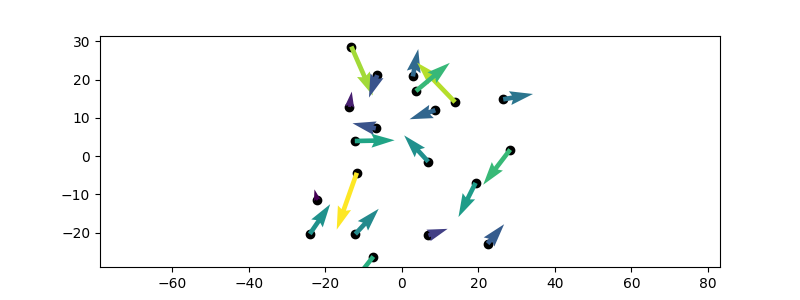
\includegraphics[width=0.5\linewidth]{tcc//img/20corpos_E_nula.png}
        \caption{Posições e momentos do problema-modelo \ref{probmodelo:20corpos_energia0}.}
        \label{fig:probmodelo_20corpos}
    \end{figure}
\end{probmodelo}

\begin{probmodelo}[100 corpos]\label{probmodelo:100corpos_energia0}
    Trata-se de um problema com $N=10^2$, todas as integrais primeiras nulas e massas iguais a $10^{-2}$. As posições e momentos lineares podem ser visualizados na figura \ref{fig:probmodelo_100corpos}.
    \begin{figure}[H]
        \centering
        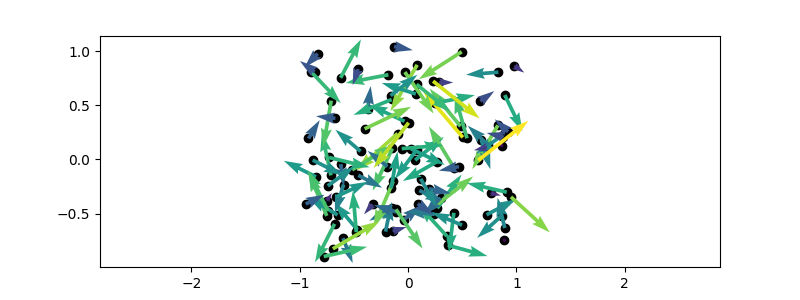
\includegraphics[width=0.5\linewidth]{tcc//img/100corpos_E_nula.png}
        \caption{Posições e momentos do problema-modelo \ref{probmodelo:100corpos_energia0}.}
        \label{fig:probmodelo_100corpos}
    \end{figure}
\end{probmodelo}

\begin{probmodelo}[1000 corpos e $E=-0.25$]\label{probmodelo:1000corpos_energianegativa}
    Trata-se de um problema com $N=10^3$, $E=-0.25$, todas as outras integrais primeiras nulas e massas iguais a $10^{-3}$.
    As posições e momentos lineares podem ser visualizados na figura \ref{fig:probmodelo_1000corpos_E_negativa}.
    \begin{figure}[H]
        \centering
        \includegraphics[width=0.5\linewidth]{tcc//img/1000corpos_E_negativa.png}
        \caption{Posições e momentos do problema-modelo \ref{probmodelo:1000corpos_energianegativa}.}
        \label{fig:probmodelo_1000corpos_E_negativa}
    \end{figure}
\end{probmodelo}

\begin{probmodelo}[1000 corpos e $E=0$]\label{probmodelo:1000corpos_energianula}
    Trata-se de um problema com $N=10^3$, todas as integrais primeiras nulas e massas iguais a $10^{-3}$. As posições e momentos lineares podem ser visualizados na figura \ref{fig:probmodelo_1000corpos_E_nula}.
    \begin{figure}[H]
        \centering
        \includegraphics[width=0.5\linewidth]{tcc//img/1000corpos_E_nula.png}
        \caption{Posições e momentos do problema-modelo \ref{probmodelo:1000corpos_energianula}.}
        \label{fig:probmodelo_1000corpos_E_nula}
    \end{figure}
\end{probmodelo}

\begin{probmodelo}[1000 corpos e $E=0.25$ (massas iguais)]\label{probmodelo:1000corpos_energiapositiva_1}
    Trata-se de um problema com $N=10^3$, $E=0.25$, todas as outras integrais primeiras nulas e massas iguais a $10^{-3}$. As posições e momentos lineares podem ser visualizados na figura \ref{fig:probmodelo_1000corpos_E_positiva_1}.
    \begin{figure}[H]
        \centering
        \includegraphics[width=0.5\linewidth]{tcc//img/1000corpos_E_positiva_1.png}
        \caption{Posições e momentos do problema-modelo \ref{probmodelo:1000corpos_energiapositiva_1}.}
        \label{fig:probmodelo_1000corpos_E_positiva_1}
    \end{figure}
\end{probmodelo}

\begin{probmodelo}[1000 corpos e $E=0.25$ (massas diferentes)]\label{probmodelo:1000corpos_energiapositiva_2}
    Trata-se de um problema com $N=10^3$, $E=0.25$, todas as outras integrais primeiras nulas e massas diferentes. As posições e momentos lineares podem ser visualizados na figura \ref{fig:probmodelo_1000corpos_E_positiva_2}.
    \begin{figure}[H]
        \centering
        \includegraphics[width=0.5\linewidth]{tcc//img/1000corpos_E_positiva_2.png}
        \caption{Posições e momentos do problema-modelo \ref{probmodelo:1000corpos_energiapositiva_2}.}
        \label{fig:probmodelo_1000corpos_E_positiva_2}
    \end{figure}
\end{probmodelo}

\chapter{Demonstrações de propriedades da Dinâmica de Formas}\label{apendice:demonstracoes_dinamica_de_formas}

Em vias de facilitar a leitura e compreensão da teoria da Dinâmica de Formas para o PNCG, algumas demonstrações não foram apresentadas no corpo do texto. Porém, como tratam-se de resultados importantes para a teoria e cuja demonstração não foi publicada na literatura, vale apresentá-las neste apêndice.

\begin{proposition}[Equação \ref{eq:new_constraints}]\label{prop:new_constraints}
    Para as coordenadas objetivas $(\vet \sigma, \vet \pi)$, valem as propriedades
    \begin{align}
        \sum_{a=1}^N \vet \sigma_a \cdot \vet \sigma_a = 1, \quad
        \sum_{a=1}^N \vet \pi^a \cdot \vet \sigma_a = 0, \nonumber \\
        \sum_{a=1}^N \sqrt{m_a} \vet \sigma_a = 0, \quad
        \sum_{a=1}^N \sqrt{m_a} \vet \pi^a = 0.
    \end{align}
\end{proposition}
\begin{Proof}
    \begin{flalign*}
        \sum_{a=1}^{N} \vet \sigma_a \cdot \vet \sigma_a
        = \dfrac{1}{R^2} \sum_{a=1}^{N} m_a \vet q_a \cdot \vet q_a
        = \dfrac{R^2}{R^2} = 1.&&
    \end{flalign*}
    \begin{flalign*}
        \sum_a \vet \pi^a \cdot \vet \sigma_a
        = \dfrac{\cancel R}{D_0} \dfrac{1}{\cancel R} \sum_a \dfrac{\vet p^a_{cm}}{\cancel{\sqrt{m_a}}} \cancel{\sqrt{m_a}} \vet q_a^{cm} - \dfrac{D}{D_0} \sum_a \vet \sigma_a \cdot \vet \sigma_a
        = \dfrac{D}{D_0} - \dfrac{D}{D_0} = 0.&&
    \end{flalign*}
    \begin{flalign*}
        \sum_a \sqrt{m_a} \vet \sigma_a 
        = \dfrac{1}{R} \sum_a m_a \vet q_a
        = \dfrac{1}{R} \sum_a m_a \vet q_a
        = \vet 0.&&
    \end{flalign*}
    \begin{flalign*}
        \sum_a \sqrt{m_a} \vet \pi^a 
        = \dfrac{R}{D_0} \sum_a \dfrac{\sqrt{m_a}}{\sqrt{m_a}}\vet p^a - \dfrac{D}{D_0} \sum_a \sqrt{m_a} \vet \sigma_a
        = \vet 0.&&
    \end{flalign*}
\end{Proof}

\begin{proposition}[Invariância por escala, equação \ref{eq:invariancia_por_escala}]\label{prop:invariancia_por_escala}
    As coordenadas objetivas $(\vet \pi, \vet \sigma)$ são invariantes por escala, pois comutam com $D$ e com $R$,
    \begin{equation*}
        \{ f(D, R), \vet \pi_a \} = \{ f(D,R), \vet \sigma_a \} = 0.
    \end{equation*}
\end{proposition}
\begin{Proof}
    Primeiro, observe que $\vet x$ comutar com $f(D, R)$ equivale a $\vet x$ comutar com $D$ e com $R$:
    \begin{align*}
        \{ f(D,R), \vet x \}
        &= \sum_a \derpar{f(D,R)}{\vet q_a} \cdot \derpar{\vet x}{\vet p^a} - \derpar{f(D,R)}{\vet p^a} \cdot \derpar{\vet x}{\vet q_a} 
        \\
        &= \sum_a \left[ \derpar{f}{D} \derpar{D}{\vet q_a} + \derpar{f}{R} \derpar{R}{\vet q_a} \right] \derpar{\vet x}{\vet p^a} - \left[ \derpar{f}{D} \derpar{D}{\vet p^a} + \derpar{f}{R} \derpar{R}{\vet p^a} \right] \derpar{\vet x}{\vet q_a}
        \\
        &= \derpar{f}{D} \sum_a \left[\derpar{D}{\vet q_a} \derpar{\vet x}{\vet p^a} - \derpar{D}{\vet p^a} \derpar{\vet x}{\vet q_a} \right] + \derpar{f}{R} \sum_a \left[\derpar{R}{\vet q_a} \derpar{\vet x}{\vet p^a} - \derpar{R}{\vet p^a} \derpar{\vet x}{\vet q_a} \right] 
        \\
        &= \derpar{f}{D} \{D, \vet x\} + \derpar{f}{R} \{R, \vet x\}.
    \end{align*}
    Assim, basta verificar as comutatividades individuais. Temos as derivadas parciais:
    \begin{align*}
        \derpar{\vet \sigma_a}{\vet q_b} = \dfrac{\sqrt{m_a}}{R^2}\left(\delta_a^b R - \dfrac{m_b}{R} \vet q_a \cdot \vet q_b\right),
        \quad
        \derpar{\vet \sigma_a}{\vet p_b} = 0,
        \quad
        \derpar{\vet \pi^a}{\vet p_b} = \dfrac{R}{\sqrt m_a} \delta_a^b - \vet q_b \cdot \vet \sigma_a,
        \\
        \derpar{\vet \pi^a}{\vet q_b} = \dfrac{m_b}{\sqrt{m_a}} R  \vet p^a \cdot \vet q_b - \vet p^a \cdot \vet \sigma_a - \dfrac{D \sqrt{m_a}}{R^2} \left( \delta_a^b R - \dfrac{m_b}{R} \vet q_a \cdot \vet q_b \right).
    \end{align*}
    Então:
    \begin{flalign*}
        \{D, \vet \sigma_a \} 
        &= \sum_i \vet p^i \derpar{\vet \sigma_a}{\vet p^i} - \vet r_i \derpar{\vet \sigma_a}{\vet r_i}
        = - \sum_i \vet r_i \dfrac{\sqrt{m_a}}{R^2}\left( \delta_a^i R - \dfrac{m_i}{R} \vet q_a \cdot \vet r_i \right)&&
        \\
        &= - \dfrac{\sqrt{m_a}}{R} \vet q_a + \dfrac{\sqrt{m_a}}{R} \vet q_a \sum_i \dfrac{m_i \vet r_i \cdot \vet r_i}{R^2} 
         = - \dfrac{\sqrt{m_a}}{R} \vet q_a + \dfrac{\sqrt{m_a}}{R} \vet q_a \sum_i \vet \sigma_i \cdot \vet \sigma_i = 0.&&
    \end{flalign*}
    \begin{flalign*}
        \{R, \vet \sigma_a \} = 
        \sum_i \derpar{R}{\vet r_i} \derpar{\vet \sigma_a}{\vet p^i} - \derpar{R}{\vet p^i} \derpar{\vet \sigma_a}{\vet r_i} = 0.&&
    \end{flalign*}
    \begin{flalign*}
        \{D, \vet \pi^a \} 
        &= \sum_i \vet p^i \left( \dfrac{R}{\sqrt{m_a}}\delta_a^i - \vet r_i \vet \sigma_a \right) - \vet r_i \derpar{\vet \pi_a}{\vet q_i} 
        = \vet \pi^a - \dfrac{R}{\sqrt{m_a}} \vet p^a \sum_i \norma{\vet \sigma_i}^2 - \dfrac{D\sqrt{m_a}}{R} \vet q_a \sum_i \norma{\sigma_i}^2 &&
        \\ 
        &= \vet \pi^a - \dfrac{R}{\sqrt{m_a}} \vet p^a - \dfrac{D \sqrt{m_a}}{R} \vet q_a
        = \vet \pi^a - \vet \pi^a = 0. &&
    \end{flalign*}
    \begin{flalign*}
        \{R, \vet \pi^a\} 
        &= \sum_i \derpar{R}{\vet r_i} \derpar{\vet \pi^a}{\vet p^i} - \derpar{R}{\vet p^i}\derpar{\vet \pi^a}{\vet r_i}
         = \sum_i \dfrac{m_i \vet r_i}{R} \left( \dfrac{R}{\sqrt{m_a}} \delta_a^i - \vet r_i \vet \sigma_a \right) &&
         \\
        &= \sqrt{m_a} \vet q_a - \vet \sigma_a \sum_i \dfrac{m_i \vet r_i \vet r_i}{R}
         = \sqrt{m_a} \vet q_a - R \vet \sigma_a \sum_i \norma{\vet \sigma_i}^2 &&
         \\
        &= R(\vet \sigma_a - \vet \sigma_a) = 0.&&
    \end{flalign*}
    Assim, obtivemos que
    \begin{equation*}
        \{D, \vet \sigma_a\} = \{D, \vet \pi^a \} = \{R, \vet \sigma_a\} = \{R, \vet \pi^a\} = 0.
    \end{equation*}
\end{Proof}

\par

% %%%% Anexos %%%%

% \makeatletter
% \if@openright\cleardoublepage\else\clearpage\fi
% \makeatother

% \pagestyle{appendix} % repete o anterior, caso você não use apêndices

% \annex

% % \addappheadtotoc acrescenta a palavra "Anexo" ao sumário; se
% % só há anexos, sem apêndices, provavelmente não é necessário.
% \addappheadtotoc

% \par
% \input{tcc/apendices/codigos}

%%%%%%%%%%%%%%% SEÇÕES FINAIS (BIBLIOGRAFIA E ÍNDICE REMISSIVO) %%%%%%%%%%%%%%%%
% O comando backmatter desabilita a numeração de capítulos.
\backmatter

\pagestyle{backmatter}

% Espaço adicional no sumário antes das referências / índice remissivo
\addtocontents{toc}{\vspace{2\baselineskip plus .5\baselineskip minus .5\baselineskip}}

% A bibliografia é obrigatória

\printbibliography[
  title=\refname\label{bibliografia}, % "Referências", recomendado pela ABNT
  %title=\bibname\label{bibliografia}, % "Bibliografia"
  heading=bibintoc, % Inclui a bibliografia no sumário
]

% ÍNDICE REMISSIVO
% \printindex % imprime o índice remissivo no documento (opcional)


\end{document}